This chapter describes the first differential cross-section measurement at ATLAS of the electroweak production of a W boson and a photon in association with two jets. The research detailed in this chapter is included in a paper submitted to journal and publicly available at \cite{VBSWy:VBSWy}, where the differential cross-section measurements are used to derive constraints on dimension-8 operators in the context of an effective field theory (EFT). The paper also describes the observation and fiducial cross-section measurements of this process. The CMS collaboration has previously reported the observation \cite{VBSWy:CMSVBSWy} and differential cross-section measurements of this process \cite{VBSWy:CMSdiffx}. The ATLAS paper is the first to publish constraints on the $f_{T3}$ and $f_{T4}$ operators\footnote{The dimension-8 $T$ operators are given by the different ways of contracting the SU(2) and U(1) field strength tensors, and represent anomalous quartic gauge interactions involving a $\gamma$ and a $W$, without trilinear interactions. The T3 and T4 operators were only added to dimension-8 EFT models in March 2021, and have therefore remained unconstrained by measurements prior to this analysis \cite{TtypeOperators}.} and also gives differential cross-section measurements of observables sensitive to CP-violating (CPV) Higgs and weak boson interactions. The work shown in this chapter is the authors own except when explicitly stated otherwise.
%Unfolded differential cross-sections for \ewwy production in 6 different observables are derived. These are the dijet invariant mass \mjj, dijet transverse momentum \jjpt, signed\footnote{Signed here refers to the fact that the jets are rapidity ordered before subtracting the azimuthal angles. This makes these observables parity-odd.} dijet azimuthal angle separation \jjdphi, lepton transverse momentum \leppt, signed azimuthal angle separation of the lepton and the photon \lepgamdphi, and the invariant mass of the lepton-photon system \lym. \mjj is measured for the reason that it characterises the EW measurement -- \mjj is one of the most important observables used to discriminate the QCD production mode from the EW mode in VBS/VBF processes. \ptjj probes the kinematics of the forward jet system, and is expected to be more sensitive to dim-8 EFT contributions than \mjj. The \leppt and \lym observables probe the kinematics of the central diboson system. %The mass of this system has been shown to be very sensitive to dim-8 EFT contributions in other VBS/VBF analyses \textcolor{red}{citation needed}. 

Unfolded differential cross-sections for \ewwy production are measured for 6 different observables. These are the dijet invariant mass \mjj, dijet transverse momentum \jjpt, signed dijet azimuthal angle separation \jjdphi, lepton transverse momentum \leppt, signed azimuthal angle separation of the lepton and the photon \lepgamdphi, and the invariant mass of the lepton-photon system \lym. The signed nature of the angular observables refers to the fact that the objects are rapidity ordered before subtracting the azimuthal angles. i.e. 
\begin{equation}
  \Delta\phi_{ij}=\phi^i_f-\phi^j_b, \hspace{5pt}\text{where}\hspace{5pt} y^i_f>y^j_b.
\end{equation}
The dijet invariant mass is one of the most important observables used to discriminate the strong production mode from the EW mode in VBS/VBF processes, in this way \mjj characterises the VBS measurement. The dijet transverse momentum probes the kinematics of the forward jet system. Preliminary EFT studies showed that \ptjj is expected to be more sensitive to dim-8 EFT contributions than \mjj. The \leppt and \lym observables probe the kinematics of the central diboson system. %The mass of this system has been shown to be very sensitive to dim-8 EFT contributions in other VBS/VBF analyses \textcolor{red}{citation needed}. 
Finally, the angular observables \jjdphi and \lepgamdphi are expected to be sensitive to CPV gauge couplings contributing to the $WW\gamma\gamma$ and $WW\gamma Z$ vertices. The \ewwy differential cross-section paper \cite{VBSWy:VBSWy} does not publish limits on these couplings as they still need to be included in EFT models in MC event generators, but the published results may help future analyses looking to derive these limits. 

\section{Signal and Background Processes}

%The nominal sample for \ewwy production is generated using \MGNLO (v.2.6.5), with LO matrix-element (ME) accuracy in perturbative QCD, where the \NNPDFlo PDF set is used in the calculation of the matrix element. The ME-level final state is interfaced with \PYTHIA (v8.240) with dipole recoil turned on for generating the parton shower (PS) and UE, using the A14 tuned parameter set for the modelling of non-perturbative effects. \EVTGEN (v1.6.0) is used for the properties of b- and c- hadron decays. An additional \ewwy sample is generated using \SHERPA2.2.12, with LO matrix element accuracy, where the \NNPDF PDF set is used, where the tuned parameter set used in the PS, UE, and hadronisation is default one developed by the \SHERPA authors. The ME calculation is performed for up to one parton using the internal ME generator \COMIX, and the ME is merged with parton showers for events with two or three partons using the \MEPSatLO prescription. All partons are treated as massless at the ME calculation, and massive in the parton shower, and diagrams involving initial state b quarks are explicitly excluded in the ME calculation, as these diagrams are covered by seperate single-top MC samples\footnote{With this setup, diagrams involving the t-channel exchange of a $Z$-boson via a b-quark are excluded from the analysis. Seperate studies have shown that this has a negligible impact. \textcolor{red}{STILL NEEDS TO BE VERIFIED}}. The parton showering is conducted by \CSShower, which is based on Catani-Seymour dipole factorisation.

\subsection{Signal}

The nominal sample for the EW production mode of $l\nu\gamma$jj (referred to as \ewwy in this chapter) is generated using \SHERPA2.2.12 \cite{Insitu:sherpa,Insitu:sherpa22}, with LO matrix element accuracy, where the \NNPDF PDF set \cite{Insitu:nnpdf} is used, and the tuned parameter set used in the parton shower (PS), underlying event (UE), and hadronisation is the default one developed by the \SHERPA authors. The ME calculation is performed for up to three partons in the finals state using the internal ME generator \COMIX \cite{Insitu:comix}, and the ME is merged with the PS for events using the \MEPSatLO prescription \cite{Insitu:meps}. All partons are treated as massless in the ME calculation, and massive in the PS, and diagrams involving initial state $b$-quarks are explicitly excluded in the ME calculation, as these diagrams are covered by separate single-top MC samples\footnote{With this setup, diagrams involving the t-channel exchange of a $Z$-boson via a b-quark are excluded from the analysis. Separate studies have shown that this has a negligible impact.}. The PS is conducted by \CSShower \cite{Insitu:csshower}, which is based on Catani-Seymour dipole factorisation \cite{Insitu:csalgorithm}. 

An additional \ewwy sample is generated using \MGNLO (v.2.6.5) \cite{VBSWy:madgraph}, with LO matrix-element (ME) accuracy in perturbative QCD, where the \NNPDFtwolo \cite{Insitu:nnpdf} PDF set is used in the calculation of the ME. The ME calculation is performed for two partons in the final state. The ME-level final state is interfaced with \PYTHIA (v8.240) \cite{Insitu:pythia} with dipole recoil turned on for generating the PS and UE, using the A14 \cite{VBSWy:a14} tuned parameter set for the modelling of non-perturbative effects. \EVTGEN (v1.6.0) \cite{Insitu:evtgen} is used for the properties of $b$- and $c$-hadron decays. The \SHERPA sample has 4783000 total events, whereas the \MGNLO sample has 5013000 total events. The \SHERPA sample is used as the nominal MC sample since the ME calculation is performed for up to three partons, compared to 2 partons (i.e. no extra emissions) in the \MGNLO sample.

It is worth commenting on the fact that LO samples are used for the simulations of the signal process. The current state-of-the-art for the MCnet MC generators are LO-merged samples, such as the \SHERPA \ewwy sample used in this analysis. The NLO calculation for $V\gamma jj$ processes is extremely challenging because of the interference with the strong $V\gamma jj$ process and the presence of infrared singularities from NLO correction to both the electroweak and strong diagrams \cite{VBSWy:VBSNLO,VBSWy:MCNetVBSNLO}. 
%The choice of the \SHERPA sample as the nominal one is based on the fact that the ME is calculated with up to three partons, compared to two partons for the \MGNLO sample.
\subsection{Backgrounds}

\subsubsection{Strong $W\gamma$jj}
The nominal irreducible background sample for the strong production mode of $l\nu\gamma$jj (referred to as \qcdwy in this chapter) is generated using \SHERPA2.2.11 \cite{Insitu:sherpa,Insitu:sherpa22}. The sample is produced with NLO accurate MEs for up to one parton in the final state, LO accuracy MEs for up to 3 partons in the finals state are calculated with \AMEGIC \cite{VBSWy:amegic} and \COMIX \cite{Insitu:comix}. Partons are treated as massless in the ME calculation, and massive in the PS. The PS is conducted with \CSShower \cite{Insitu:csshower}. The matrix elements are matched to the PS, and different jet multiplicities are merged using the CKKW matching procedure \cite{Insitu:ckkw1,Insitu:ckkw2}, which is extended to NLO accuracy using the \MEPSatNLO \cite{Insitu:meps} prescription. The \NNPDF \cite{Insitu:nnpdf} PDF set is used and the dedicated set of tuned parameters for the PS is developed by the \SHERPA authors. 

An alternate \qcdwy background sample is generated using \MGNLO (v2.8.1) \cite{VBSWy:madgraph} with NLO ME accuracy up to one parton in the final state. The \NNPDF PDF set is used in the calculation. The partonic final state is interfaced with \PYTHIA (v8.244) \cite{Insitu:pythia}, and the A14 \cite{VBSWy:a14} set of tuned parameters is used for PS, hadronisation and UE activity. \EVTGEN (v1.7.0) \cite{Insitu:evtgen} is used for the properties of $b$- and $c$-hadron decays.

118997000 events were generated for the \MGNLO sample, and 116239203 for the \SHERPA sample. The \SHERPA sample is chosen as the nominal MC sample. This choice is made because of the superior statistical precision of the expected number of events after the event selection described in Section \ref{sec:vbswy:evsel}. By comparing the statistical uncertainties on the total expected yields calculated using $\sqrt{\sum_iw_i^2}$, where $w_i$ are the MC event weights, the statistical precision of the \SHERPA sample was found to be 2.3 times better. The improved statistical precision arises due to a larger number of negative weights in \MGNLO.% The improved statistical precision results in lower statistical uncertainties on the extracted signal and improved statistical resolution of the systematic uncertainties. This is described in Section \ref{sec:vbswy:extraction_uncertainties}.

\subsubsection{Interference Between Strong and EW $W\gamma$jj}

In the calculation of the inclusive cross-section of W$\gamma$jj production, the electroweak and the strong scattering amplitudes can interfere. This interference is quantified in the matrix-element squared at LO as 
\begin{equation} 
|\mathcal{M}|^2 = |\mathcal{M}_{\text{EW}} + \mathcal{M}_{\text{QCD}}|^2 = |\mathcal{M}_{\text{EW}}|^2+|\mathcal{M}_{\text{QCD}}|^2+2Re(\mathcal{M}_{\text{EW}}^*\mathcal{M}_{\text{QCD}}),
\end{equation}
where $\mathcal{M}_{\text{EW}}$ and $\mathcal{M}_{\text{QCD}}$ represent the matrix elements for \ewwy and \qcdwy production, and the last term corresponds to the interference contribution. The interference must be modelled to understand its impact relative to the \ewwy differential cross-section as a function of the measurement observables.

The interference sample was modelled at LO ME accuracy using \MADGRAPH5, which was interfaced with \PYTHIA (v8.244) for PS, hadronisation, and UE activity. \EVTGEN (v1.7.0) was used for the properties of $b$- and $c$-hadron decays. This sample was generated by the author. More details about the generation of the sample and truth-level validations studies are shown in Section \ref{sec:vbswy:interference}.

\subsubsection{Prompt Backgrounds}
Backgrounds where the final state comprises at least two jets, a prompt lepton, and a prompt photon are referred to as prompt backgrounds. These include the production of top quarks in association with a prompt photon, as well as $Z\gamma$jj production.

The simulations of top backgrounds consist of:
\begin{itemize}
  \item $tt\gamma$ production. This sample is produced at LO ME accuracy. The all-hadronic $t\bar{t}$ decays are not included in this sample.
  \item $tq\gamma$, which is the t-channel production of a single top quark in association with a prompt photon, a $b-$jet, and one additional jet. This sample is produced at NLO accuracy. The s-channel diagrams have a negligible contribution since they produce two $b$-jets in the final state, and a $b$-jet veto is applied in the analysis. 
  \item $tW\gamma$ production, where the $W$ decays either hadronically or leptonically, and the photon comes from radiation off a $t$, $W$ or from their decay products. The sample is produced at LO accuracy. Diagrams where the photon is radiated from the initial state are highly suppressed as these involve additional heavy fermion internal lines.
\end{itemize}

All of the top background samples are simulated with the same event generation, showering, and hadronisation setup. They are generated with \MGNLO for the ME calculation, where the \NNPDFtwolo PDF set is used. The ME-level final state is interfaced with \PYTHIA for hadronisation, showering and UE activity, and the A14 set of tuned parameters is used. \EVTGEN is used for the properties of $b$- and $c$-hadron decays. 

The $Z\gamma$ backgrounds consist of:
\begin{itemize}
  \item Strong-$Z\gamma$jj production, which include separate samples for $e,\mu,\tau,\nu$ channels. MEs are calculated with \SHERPA 2.2.11 at NLO QCD accuracy for up to one additional parton, and LO accuracy for up to three additional partons.
  \item EW-$Z\gamma$jj production with a t-channel requirement to suppress triboson final states. The ME is calculated with \SHERPA 2.2.12 at LO accuracy for up to one additional parton. Diagrams with initial state $b$-quarks are explicitly excluded. 
\end{itemize}
The treatment of parton shower, hadronisation and underlying event is the same as the $W\gamma$jj samples. The \NNPDF PDF sets are used.
\subsubsection{Non-prompt backgrounds}
Background events can arise from non-prompt leptons or photons in association with jets. Additionally, electrons can be mis-reconstructed as photons (referred to as \efakey backgrounds), and jets can be mis-reconstructed as photons (\jfakey) or leptons (\jfakee, \jfakemu). The contributions from these backgrounds are estimated using data-driven methods as described in Section \ref{sec:vbswy:nonprompt}. %These backgrounds are collectively referred to as non-prompt backgrounds in this chapter. The MC samples used for the non-prompt background estimates are 
%\begin{itemize}
%  \item $W$+jets -- used in \jfakey validation.
%  \item $Z$+jets -- used in \jfakey validation, \efakey estimate.
%  \item $tW$ -- used in \efakey estimate.
%  \item $t\bar{t}$ -- used in \efakey estimate.
%  \item diboson -- used in \jfakee estimate, \jfakemu estimate.
%  \item multijet -- used in \jfakee estimate, \jfakemu estimate.
%\end{itemize}
%$W$+jets and $Z$+jets samples are produced at NLO ME accuracy (up to 3 jets at NLO, 5 at LO) using \SHERPA2.2.11 using the \NNPDF PDF set and default tuning for hadronisation, PS, and UE activity. $tW$ and $t\bar{t}$ are generated at NLO ME accuracy using \POWHEG \cite{Insitu:powheg1,Insitu:powheg2,Insitu:powheg3} with the \NNPDF PDF set and \PYTHIA with A14 tuned parameters for hadronisation, PS, and UE activity. The diboson sample (0,1 additional jets at NLO; 2,3 additional jets at LO) is generated at NLO ME accuracy with \SHERPA2.2.2 using the \NNPDFnlo PDF set, and default tuning for hadronisation, PS, and UE activity. The multijet sample is generated with \PYTHIA at LO ME accuracy using the \NNPDFtwolo PDF set and A14 tuning for hadronisation, PS, and UE. 

The \GEANT toolkit \cite{GEANT4} is used for detailed modelling of the ATLAS detector response. These simulations are compared to a dataset of $pp$ collisions during the 2015-2018 data-taking period. 

%\subsubsection{Derivations and Triggers}
%
%STDM4 DAOD datasets were used which has single-lepton trigger requirements, and skimming to select for events with at least one electron with $\pt\geq20\GeV$ or at least one muon with $\pt\geq20\GeV$ within the $|\eta|<2.6$ acceptance. The \GEANT toolkit \cite{GEANT4} is used for detailed modelling of the ATLAS detector response. These simulations are compared to a dataset of $pp$ collisions during the 2015-2018 data-taking period. The data are required to pass unprescaled single lepton triggers. These triggers are listed in Table \ref{tab:vbswy:trigger}. The data are required to pass data-quality criteria to ensure the data were taken during periods where the detector subsystems were fully functioning. This is achieved via ``GoodRunsLists (GRLs)'', which are provided by the ATLAS Data Quality group. 
%
%\begin{table}[t]
%\centering
%\begin{tabular}{|c||c|c|c|}
%\hline
%& \textbf{Year} & \textbf{Level1} & \textbf{HLT} \\ \hline \hline
%\multirow{17}{*}{\textbf{Single electron trigger}} 
%& \multirow{3}{*}{2016/2017/2018} & $\et>22\GeV(*)$; & $\et>26\GeV$; \\ & & Hadronic activity veto; & tight ID, $d0$ unused; \\ & & Isolated & loose isolation
%\\ \cline{2-4} & \multirow{3}{*}{2016/2017/2018} & $\et>24\GeV(*)$; & \multirow{2}{*}{$\et>60\GeV$;} \\ & & Hadronic activity veto; & \multirow{2}{*}{medium ID, $d0$ unused} \\ & & Isolated & 
%\\ \cline{2-4} & \multirow{3}{*}{2016/2017/2018} & $\et>24\GeV(*)$; & \multirow{2}{*}{$\et>140\GeV$;} \\ & & Hadronic activity veto; & \multirow{2}{*}{loose ID, $d0$ unused} \\ & & Isolated &
%\\ \cline{2-4} & \multirow{2}{*}{2015} & $\et>20\GeV(*)$; & $\et>24\GeV$; \\ & & Hadronic activity veto & medium ID 
%\\ \cline{2-4} & \multirow{3}{*}{2015} & $\et>22\GeV(*)$; & \multirow{2}{*}{$\et>60\GeV$;} \\ & & Hadronic activity veto; & \multirow{2}{*}{medium ID} \\ & & Isolated & 
%\\ \cline{2-4} & \multirow{3}{*}{2015} & $\et>22\GeV(*)$; & \multirow{2}{*}{$\et>120\GeV$;} \\ & & Hadronic activity veto; & \multirow{2}{*}{loose ID} \\ & & Isolated & 
%\\
%\hline \hline
%\multirow{6}{*}{\textbf{Single muon trigger}} 
%& \multirow{2}{*}{2016/2017/2018} & \multirow{2}{*}{$\et>20\GeV$} & $\et>26\GeV$; \\ &&&medium isolation
%\\ \cline{2-4} & \multirow{2}{*}{2016/2017/2018} & \multirow{2}{*}{$\et>20\GeV$} & \multirow{2}{*}{$\et>50\GeV$} \\ &&& 
%\\ \cline{2-4} & \multirow{2}{*}{2015} & \multirow{2}{*}{$\et>15\GeV$} & $\et>20\GeV$; \\ &&&loose isolation
%\\
%\hline
%\end{tabular}
%\caption{Triggers used in the differential cross-section measurement. Multiple triggers for the same running period are combined such that an event is accepted when it passes any one of the individual triggers. An $\eta$-dependence of the L1 trigger threshold is denoted by (*).\label{tab:vbswy:trigger}}
%\end{table}    
%
%\clearpage
\section{Interference Sample Generation and Validation Studies\label{sec:vbswy:interference}}

The goal of studying the interference contribution was to derive an initial truth-level estimate of the ratio of the number of interference events to signal events. In addition a detector-level MC sample was produced based on this study and used in assigning a systematic uncertainty due to the interference contribution. Understanding the expected interference contribution is an important task, since performing the measurement in a phase space with a large interference fraction ($\gtrapprox20-30\%$) would result in a systematic uncertainty that would surpass the dominant uncertainty, potentially rendering the signal process as unmeasurable. A truth-level interference sample comprising of 400,000 events was generated using \MADGRAPH to perform these studies.

At the stage of the analysis where these studies were performed, the final selection criteria had not yet been finalised. As a first pass for a VBS-enriched kinematic region, the analysis cuts from the CMS 8\TeV \ewwy paper \cite{VBSWy:CMSVBSWy} were used to study the expected interference contribution. These selection criteria are outlined in Table \ref{tab:vbswy:interferencecuts}. These selection criteria are quite loose, with relatively soft \mjj and $p_{\text{T},j}$ cuts, and no $\Delta y(j,j)$ cut. This allows the interference contribution to be studied as a function of \mjj and $\Delta y(j,j)$ spectra.

\begin{table}[t]
  \centering
  \caption{\label{tab:vbswy:interferencecuts} Selection criteria used to analyse the interference/EW ratio. The top part of the table forms the base selection criteria. The bottom half contains the event selection criteria which are sequentially applied in Figure \ref{fig:vbswy:intcomp}. These are applied on top of the base selection criteria. The selection criteria are taken from \cite{VBSWy:CMSVBSWy}, with the $\Delta R$ cuts changed to match the ATLAS small-R jet definition.}
  \begin{tabular}{l c c c}
  \hline
  Variable & Selection \\ \hline
  $\pt^{e(\mu)}$, $|\eta^{e(\mu)}|$&> 30(25)$\GeV$, < 2.4(2.1) \\
  $\pt^{\gamma}$, $|\eta^{\gamma}|$&> 22 $\GeV$, < 1.44\\
  Number of electrons/muons; jets; photons & =1, $\geq2$, $\geq1$ \\
  $E_\mathrm{T}^{\mathrm{miss}}$&> 35 $\GeV$ \\
  $M^{W}_{\mathrm{T}}\equiv\sqrt{2\pt^{l}E_\mathrm{T}^{\mathrm{miss}}[1-\cos(\Delta\phi(l,\pt^{\mathrm{miss}}))]}$ & > 30 $\GeV$ \\
  %Number of jets & $\geq$2 \\
  $\pt^{j_1}(\pt^{j_2})$ & > 40(30) $\GeV$ \\ \hline\hline
  %Number of photons & $\geq$1 \\ \hline\hline
  $m_{jj}$ & >200 $\GeV$\\
  $|m_{e,\gamma}-m_{Z}|$ & <10 $\GeV$ \\
  $\Delta\phi(j,\pt^{\mathrm{miss}})$ & >0.4 \\
  Overlap Removal (OR) (object/against) & j/e, $\gamma$/j, $\gamma$/e($\mu$) \\
  $j_1, j_2$ bjet veto & \\
  $\Delta R(j_0,j_1)$, $\Delta R(j,\gamma)$, $\Delta R(j,e(\mu))$, $\Delta R(e(\mu),\gamma)$ & >0.4 \\
  \hline
  \end{tabular}
\end{table}  

To investigate the impact of individual cuts on the signal-to-interference fraction (EW/int), the cuts in the bottom row of Table \ref{tab:vbswy:interferencecuts} were applied sequentially, and the EW/int ratio was plotted for each combination of cuts. This is shown in Figure \ref{fig:vbswy:intcomp} for \mjj and \dyjj.

\begin{figure}[t]
\centering
\begin{subfigure}[b]{0.48\textwidth}
    \centering
    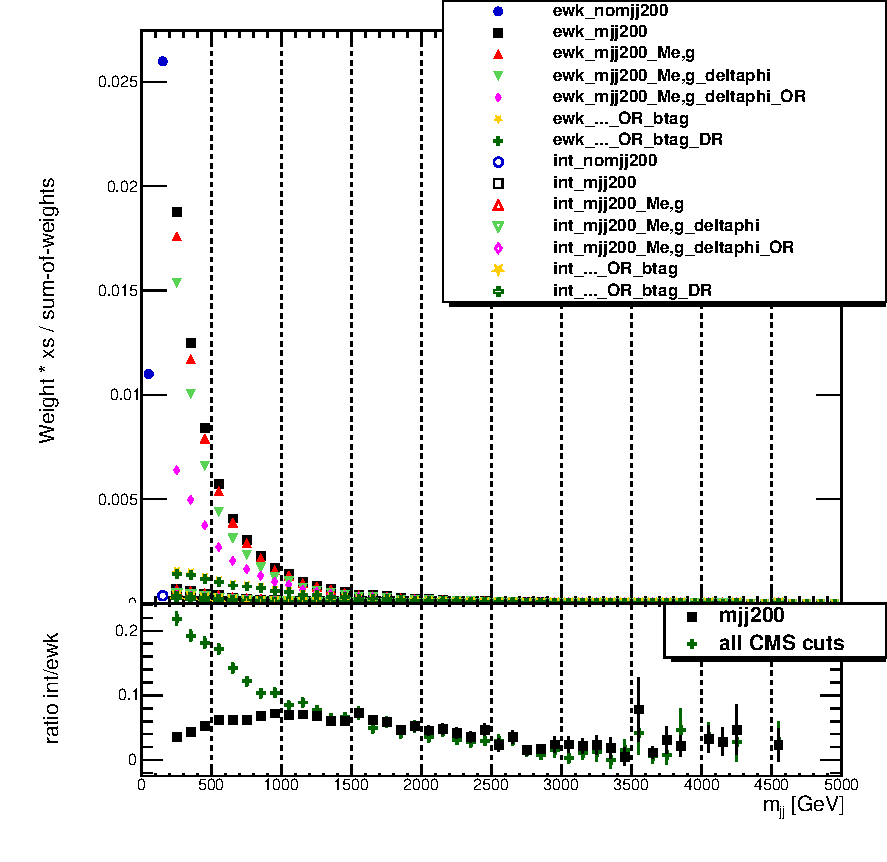
\includegraphics[width=\textwidth]{plots/diffx/mjj_comparison.pdf}
    \caption{}
    \label{fig:vbswyint:a}
\end{subfigure}
\hfill
\begin{subfigure}[b]{0.48\textwidth}
    \centering
    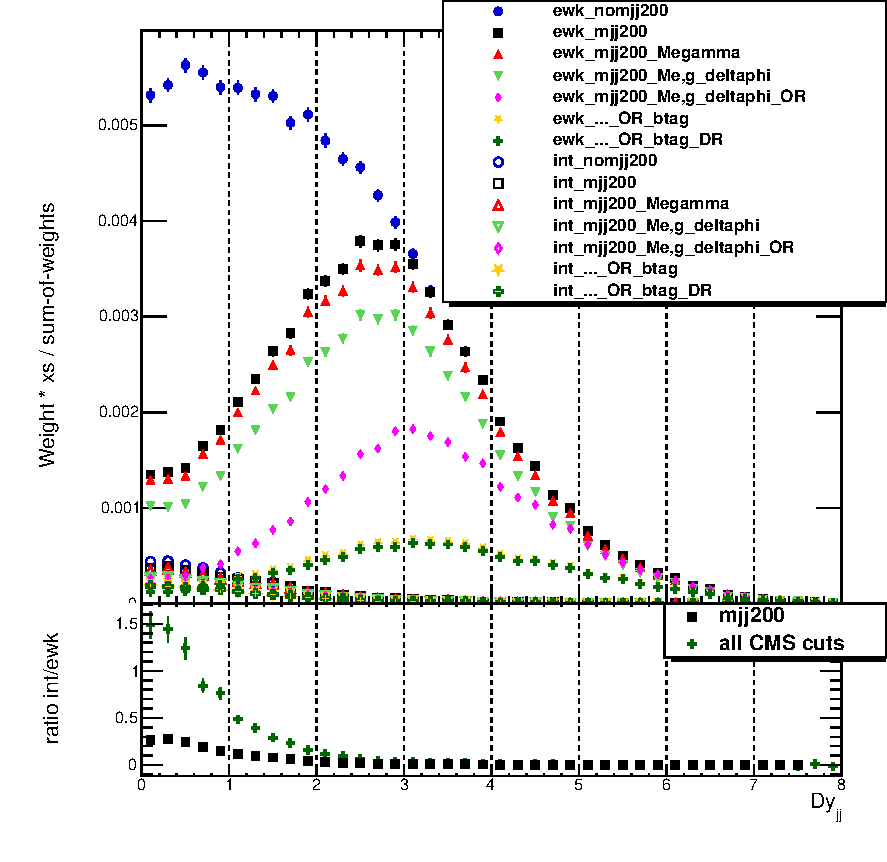
\includegraphics[width=\textwidth]{plots/diffx/dyjj_comparison.pdf}
    \caption{}
    \label{fig:vbswyint:b}
\end{subfigure}
\caption{Truth level event yields (without a luminosity factor) generated using \MADGRAPH5 for the \ewwy signal, and the interference for \mjj in (a), and \dyjj in (b). The solid markers represent the \ewwy signal, and the hollow points represent the interference. The points labelled ``\tu nomjj200'' have all the cuts applied above the two horizontal lines in Table \ref{tab:vbswy:interferencecuts}, and subsequent markers listed in the top panel legend have the additional cuts applied in Table \ref{tab:vbswy:interferencecuts}. In the ratio panel, the ``mjj200'' points have the baseline selections and the $\mjj>200\GeV$ cut applied, and the ``all CMS cuts'' points have all the baseline and additional cuts applied. There is a clear phase space dependence on the interference fraction most notably with \mjj and \dyjj selection requirements.\label{fig:vbswy:intcomp}}%From MJB documentation: NLO Powheg+Pythia 8 was known to have an issue matching jets with the parton shower, leading to poor modeling of all jet pT, as well as the recoil system pT, as seen in Figure 2 a, c, d.
\end{figure}

From Figure \ref{fig:vbswy:intcomp} it can be seen that the interference fraction is very dependent on \mjj and \dyjj. Furthermore, it is evident that applying the cuts in Table \ref{tab:vbswy:interferencecuts} increases the interference fraction significantly below $\dyjj=2$ and $\mjj=1\TeV$. Above $\dyjj=2$, the interference fraction is about 10\% at low \dyjj and drops down to 0\% at high \dyjj. Without any \dyjj cuts, the interference fraction at $\mjj=1\TeV$ is about 10\%, and this decreases at higher \mjj values. From these results it is clear that a \dyjj cut is necessary purely from in context of removing interference events. An \mjj cut of $500-1000\GeV$ would also improve the interference fraction. With these cuts, the interference fraction at truth-level is of the order of 5\% or less. This was deemed to be an acceptable interference contribution.

The generation of a detector-level interference sample has to be requested centrally, and significant computational resources are required to produce such a sample. Therefore, it is important that an appropriate number of simulated events are requested such as not to unnecessarily waste computational resources.
%
%When extracting the signal for the differential cross-section measurement (described in Section \ref{sec:vbswy:sigextraction}), the nominal signal sample is used to get a nominal extracted yield.
%In measurement of the differential cross-section, an uncertainty is assigned to the interference contribution to the \ewwy yield by repeating the signal extraction using the combination of the nominal signal sample and the interference sample (This is described in more detail in Section \ref{sec:vbswy:sigextraction}). In order for the statistical resolution of this uncertainty to be similar to the other theory uncertainties, the interference sample should have a similar statistical precision as the nominal signal sample. 

To calculate the number of simulated events required to reach a similar statistical precision as the nominal \ewwy signal sample, the number of negative weights has to be taken into account. Since the signal sample MEs are calculated at LO, the event weights are all positive and there is no penalty to the effective statistical precision due to the presence of negative weights cancelling positive weights. For the interference sample, however, there will be a significant contribution from negative event weights.

To calculate the statistical penalty due to negative event weights, we use the fact that the LO event weights are given by $\pm c$, i.e. event weights only differ by a change in sign, therefore the event weight just factorises out when calculating the statistical uncertainty:
\begin{equation}\label{eq:negweights}
  \begin{split}
  &\delta_{\text{abs}}^{\text{stat}} = \sqrt{\sum_{n_+}(+c)^2 + \sum_{n_-}(-c)^2}=c\sqrt{n_++n_-} \\
  &\delta_{\text{rel}}^{\text{stat}} = \frac{\delta_{\text{abs}}^{\text{stat}}}{(n_+-n_-)c} = \frac{\sqrt{n_++n_-}}{n_+-n_-} = \frac{1}{\sqrt{N_{\text{gen}}}}\frac{1}{1-2f_-},
  \end{split}
\end{equation} 
where $n_+$ and $n_-$ are the number of positive and negative weights, respectively; $N_{\text{gen}}\equiv n_++n_-$ is the total number of generated events; $\delta_{\text{abs}}^{\text{stat}}$ and $\delta_{\text{rel}}^{\text{stat}}$ are the absolute and relative MC statistical uncertainties; and $f_-\equiv n_-/N_\text{gen}$ is the fraction of negative weights. If $f_-=0$, the statistical precision is given by $1/\sqrt{N_{\text{gen}}}$. Therefore the effective number of events with a non-zero fraction of negative weights is given by:
\begin{equation}
  N_{\text{eff}}=(1-2f_-)^2N_{\text{gen}},
\end{equation}
i.e. the penalty to the statistical precision due to negative weights is given by $(1-2f_-)^2$.

In Figure \ref{fig:vbswy:intweights}, the fraction of negative weights is plotted with \mjj and \dyjj with cuts at $\mjj>200\GeV$; $\mjj>200\GeV, \dyjj>1$; and $\mjj>500\GeV, \dyjj>2$ in order to investigate the required number of events in different regions of phase space. The fraction of negative weights is relatively flat with \mjj and \dyjj in the three different regions. Therefore the integrated fraction of negative weights is used as the metric to determine the required statistical precision of the sample. The average integrated fraction of negative weights is $f_-=0.37$, which gives a statistical penalty of about 12, which means that the interference sample would need about 12 times the number of events to equal the statistical precision of the \MADGRAPH \ewwy signal sample. However, since the interference fraction is likely to be $<5\%$, the decision was made to request 5$\times$ the number of events.%, rather than 12, resulting in an interference sample with approximately $\sqrt{5/12}=65\%$ the statistical precision of the \MADGRAPH signal sample.

\begin{figure}[t]
\centering
%\begin{subfigure}[b]{0.32\textwidth}
%    \centering
%    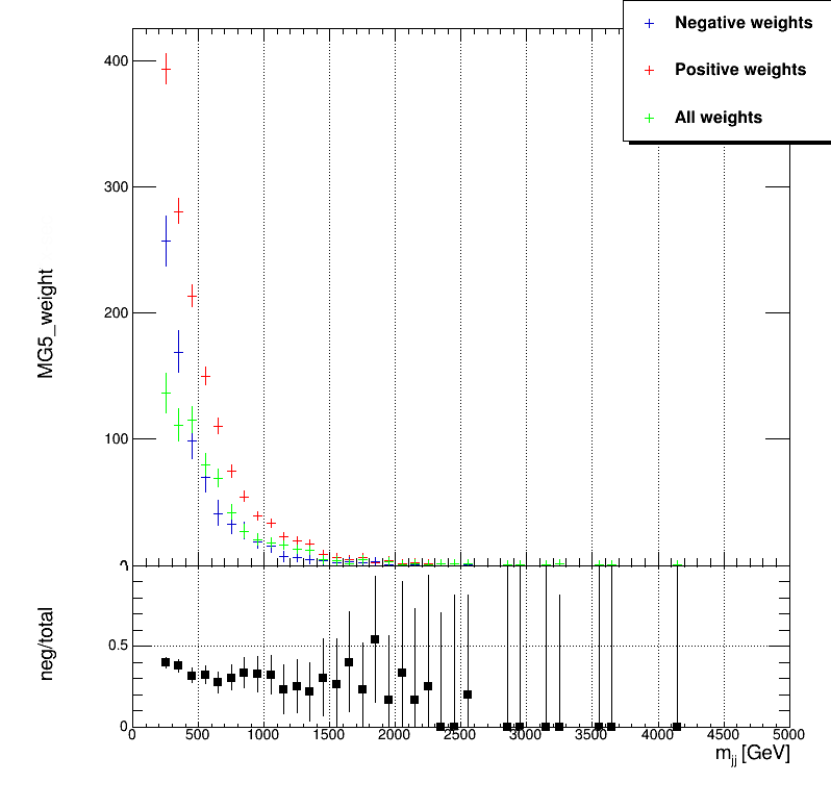
\includegraphics[width=\textwidth]{plots/diffx/int_mjj_1.png}
%    \caption{$f_-=0.34$}
%\end{subfigure}
%\hfill
%\begin{subfigure}[b]{0.32\textwidth}
%    \centering
%    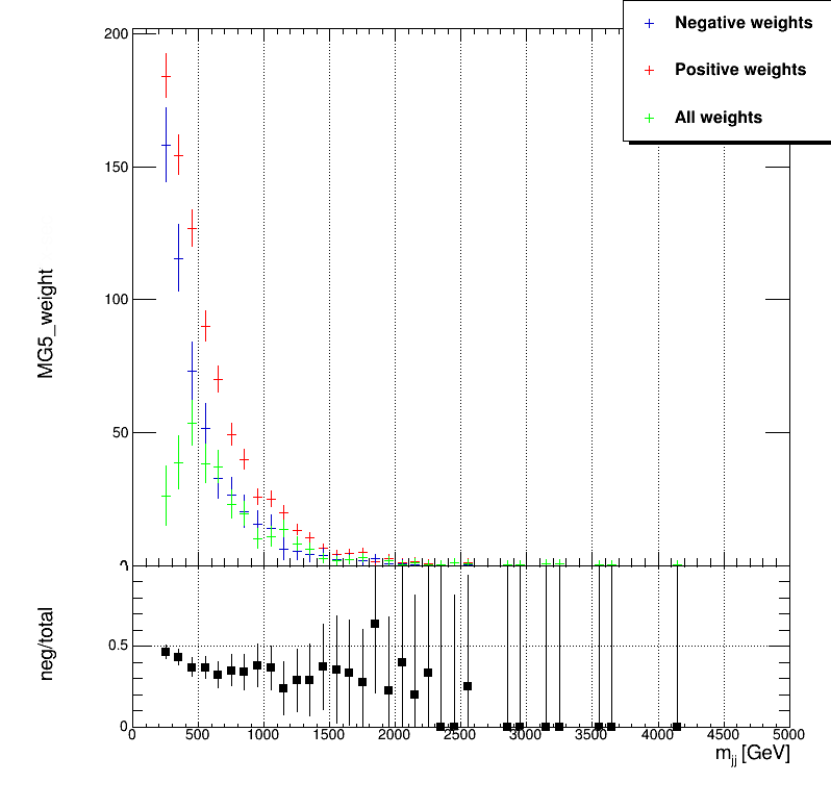
\includegraphics[width=\textwidth]{plots/diffx/int_mjj_2.png}
%    \caption{$f_-=0.39$}
%\end{subfigure}
%\hfill
\begin{subfigure}[b]{0.49\textwidth}
    \centering
    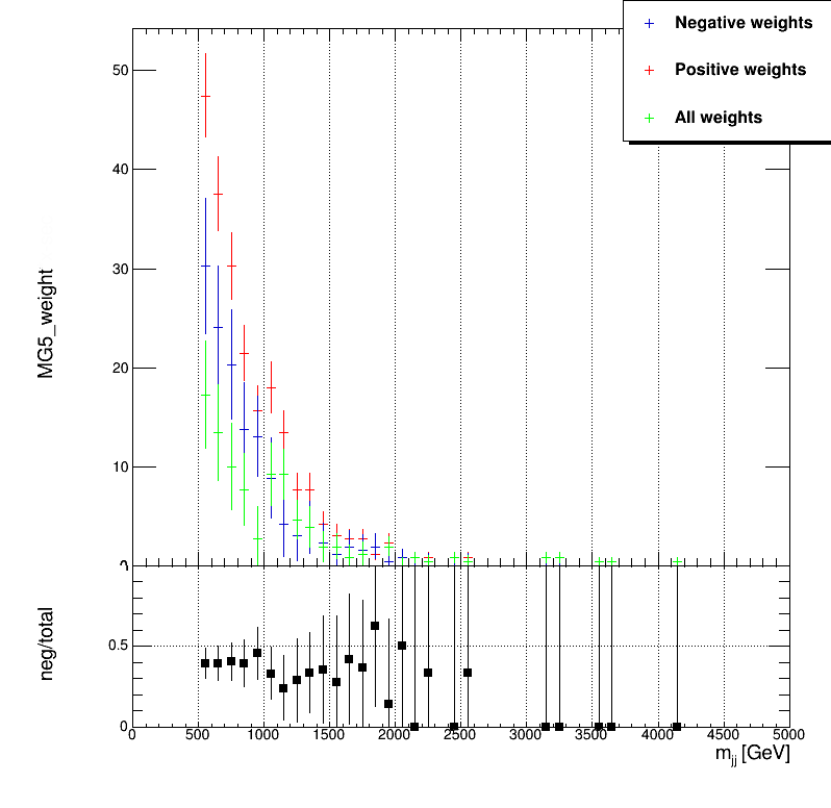
\includegraphics[width=\textwidth]{plots/diffx/int_mjj_3.png}
    \caption{$f_-=0.37$}
\end{subfigure}
\hfill
%\begin{subfigure}[b]{0.32\textwidth}
%    \centering
%    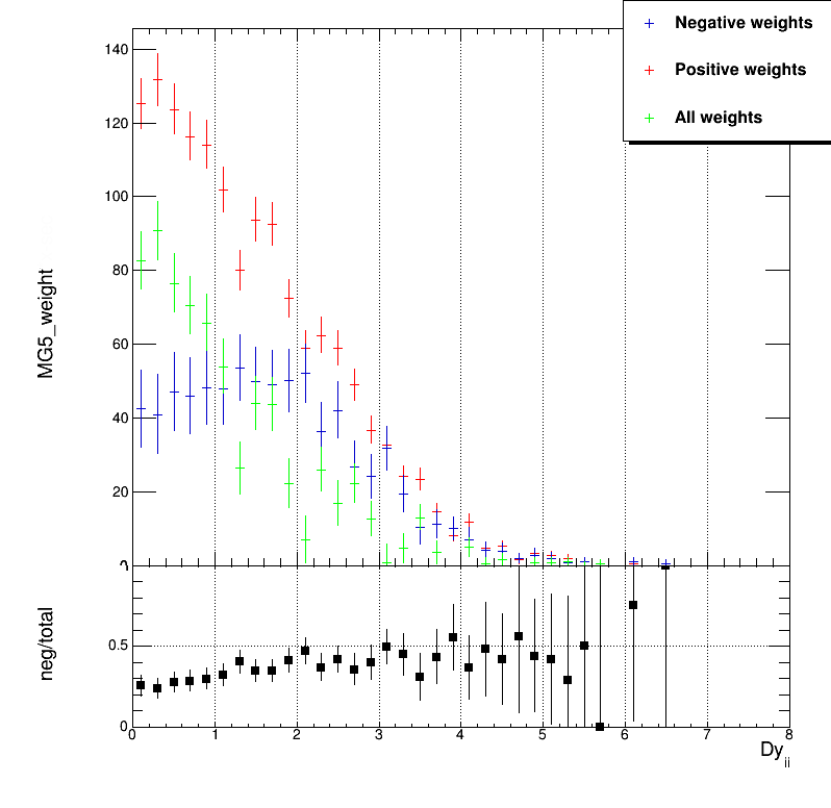
\includegraphics[width=\textwidth]{plots/diffx/int_dyjj_1.png}
%    \caption{$f_-=0.34$}
%\end{subfigure}
%\hfill
%\begin{subfigure}[b]{0.32\textwidth}
%    \centering
%    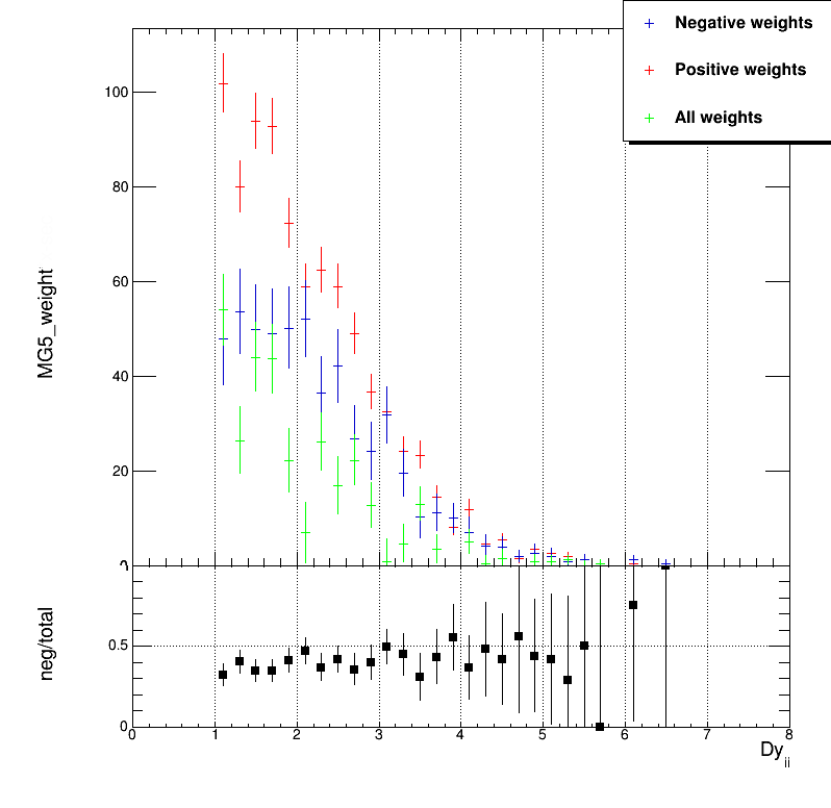
\includegraphics[width=\textwidth]{plots/diffx/int_dyjj_2.png}
%    \caption{$f_-=0.39$}
%\end{subfigure}
%\hfill
\begin{subfigure}[b]{0.49\textwidth}
    \centering
    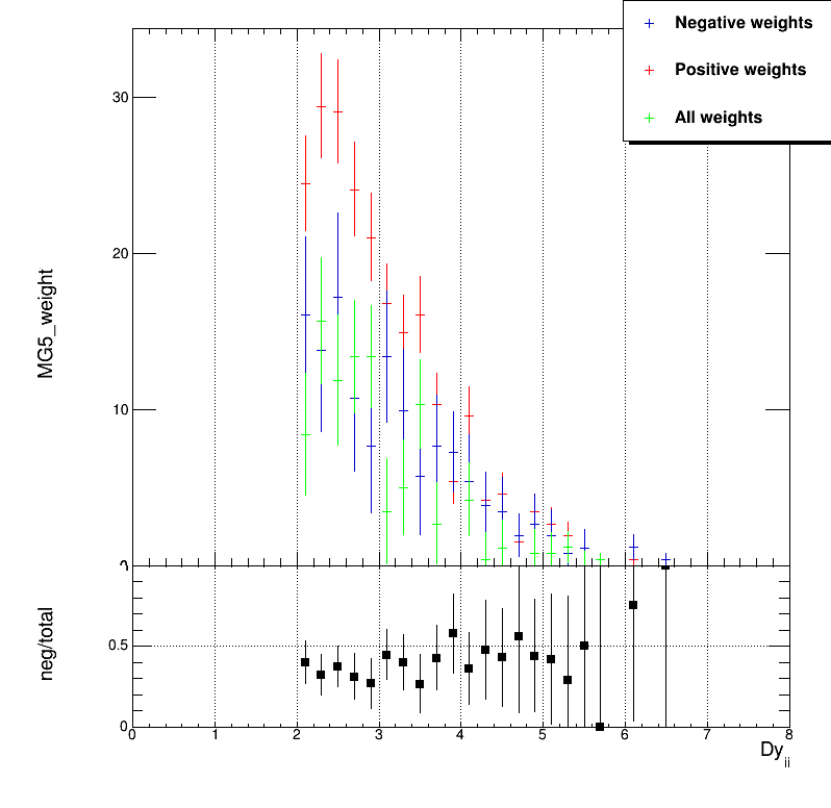
\includegraphics[width=\textwidth]{plots/diffx/int_dyjj_3.png}
    \caption{$f_-=0.37$}
\end{subfigure}
\caption{MC weights in bins of \mjj (a), and \dyjj (b) with the $\mjj>500\GeV$, $\dyjj>2$ cuts applied. The integrated fraction of negative weights is shown in the subfigure captions. The sign of the negative weights is not shown. The ratio panel shows the fraction of negative weights for a given \mjj or \dyjj bin. \label{fig:vbswy:intweights}}
\end{figure}

%\clearpage
\section{Object and Event Selections}

\subsection{Derivations and Triggers}

The analysis uses derivations which are skimmed using the preselections of passing a single-lepton trigger, and the presence of at least one lepton with $\pt\geq20\GeV$ within the $|\eta|<2.6$ acceptance. The data are required to pass un-prescaled single lepton triggers. These triggers are listed in Table \ref{tab:vbswy:trigger}. The data are required to pass data-quality criteria to ensure the data were taken during periods where the detector subsystems were fully functioning. This is achieved via ``GoodRunsLists (GRLs)'', which are provided by the ATLAS Data Quality group. 

\begin{table}[t]
\centering
\begin{tabular}{|c||c|c|c|}
\hline
& \textbf{Year} & \textbf{Level1} & \textbf{HLT} \\ \hline \hline
\multirow{17}{*}{\textbf{Single electron trigger}} 
& \multirow{3}{*}{2016/2017/2018} & $\et>22\GeV(*)$; & $\et>26\GeV$; \\ & & Hadronic activity veto; & tight ID, $d0$ unused; \\ & & Isolated & loose isolation
\\ \cline{2-4} & \multirow{3}{*}{2016/2017/2018} & $\et>24\GeV(*)$; & \multirow{2}{*}{$\et>60\GeV$;} \\ & & Hadronic activity veto; & \multirow{2}{*}{medium ID, $d0$ unused} \\ & & Isolated & 
\\ \cline{2-4} & \multirow{3}{*}{2016/2017/2018} & $\et>24\GeV(*)$; & \multirow{2}{*}{$\et>140\GeV$;} \\ & & Hadronic activity veto; & \multirow{2}{*}{loose ID, $d0$ unused} \\ & & Isolated &
\\ \cline{2-4} & \multirow{2}{*}{2015} & $\et>20\GeV(*)$; & $\et>24\GeV$; \\ & & Hadronic activity veto & medium ID 
\\ \cline{2-4} & \multirow{3}{*}{2015} & $\et>22\GeV(*)$; & \multirow{2}{*}{$\et>60\GeV$;} \\ & & Hadronic activity veto; & \multirow{2}{*}{medium ID} \\ & & Isolated & 
\\ \cline{2-4} & \multirow{3}{*}{2015} & $\et>22\GeV(*)$; & \multirow{2}{*}{$\et>120\GeV$;} \\ & & Hadronic activity veto; & \multirow{2}{*}{loose ID} \\ & & Isolated & 
\\
\hline \hline
\multirow{6}{*}{\textbf{Single muon trigger}} 
& \multirow{2}{*}{2016/2017/2018} & \multirow{2}{*}{$\et>20\GeV$} & $\et>26\GeV$; \\ &&&medium isolation
\\ \cline{2-4} & \multirow{2}{*}{2016/2017/2018} & \multirow{2}{*}{$\et>20\GeV$} & \multirow{2}{*}{$\et>50\GeV$} \\ &&& 
\\ \cline{2-4} & \multirow{2}{*}{2015} & \multirow{2}{*}{$\et>15\GeV$} & $\et>20\GeV$; \\ &&&loose isolation
\\
\hline
\end{tabular}
\caption{Triggers used in the differential cross-section measurement. Multiple triggers for the same running period are combined such that an event is accepted when it passes any one of the individual triggers. An $\eta$-dependence of the L1 trigger threshold is denoted by (*).\label{tab:vbswy:trigger}}
\end{table}    

\subsection{Object Selections}\label{sec:vbswy:objects}

\subsubsection{Photons}

Photons are reconstructed from calorimeter deposits in the second layer of the EM calorimeter as described in Section \ref{sec:egamma}. Photons are calibrated using the ``EgammaCalibrationAndSmearingTool'' with the ESModel ``es2018\tu R21\tu v0'' configuration using the decorrelation model setting ``1NP\tu v1'', corresponding to only one scale and resolution systematic variation. The ``ElectronPhotonShowerShapeFudgeTool'' is used to correct for imperfectly modelled shower shape variables. After calibration, photons are required to pass object quality, cleaning, disambiguation, and high-voltage cell removal using the corresponding tools in the ATLAS software framework. The kinematic requirement for photons is $\pt>22\GeV$. Photons are required to pass \textit{Tight} ID and \textit{FixedCutTightCaloOnly} isolation defined as $E_\text{T}^{\text{cone}40}<0.22\pt+2.45\GeV$. Scale factors are applied to simulation to correct for the disagreement in the photon selection efficiencies between data and simulation (refer to Section \ref{sec:objreco} for a description of scale factors). 

\subsubsection{Electrons}

Electrons are reconstructed from ID tracks and calorimeter information as described in Section \ref{sec:egamma}. Electrons are calibrated using the ``EgammaCalibrationAndSmearingTool'' with the ESModel ``es2018\tu R21\tu v0'' configuration and using the decorrelation model setting ``1NP\tu v1'', such that there is only one non-zero scale and resolution systematic variation. Electrons are required to satisfy a kinematic requirement of $\pt>30\GeV$, and are constrained to originate from the primary hard-scatter vertex through the impact parameter requirements $|d_0|/|\sigma_{d_0}|<5$ and $|z_0\sin\theta|<0.5\mm$. The geometrical acceptance requirements are that electrons satisfy $|\eta|<2.47$, but excluding the gap region between the barrel and endcap EM calorimeters at $1.36<|\eta|<1.52$. Electrons satisfy \textit{Tight} isolation, and \textit{Tight} ID requirements. Scale factors are applied to simulation to correct for the disagreement in the electron selection efficiencies between data and simulation. 

\subsubsection{Muons}

Muons are reconstructed from MS tracks matched to ID tracks as described in Section \ref{sec:muon}. Scale factors are applied to simulation to correct for disagreement in the muon selection efficiencies between data and simulation. Muons are calibrated using the ``MuonCalibrationAndSmearingTool'' with the ``correctData\tu IDMS'' scheme which gives muon track resolution and momentum scale systematic variations on the separate ID and MS components of the combined muon. Muons are required to satisfy \textit{Tight} ID and \textit{PflowTight\tu VarRad} isolation requirements, where the ``VarRad'' suffix refers to a shrinking isolation cone radius as high \pt. Reconstructed muons have a kinematic requirement of $\pt>30\GeV$, and are constrained to originate from the primary hard-scatter vertex through the impact parameter requirements $|d_0|/|\sigma_{d_0}|<3$ and $|z_0\sin\theta|<0.5\mm$. The geometrical acceptance requirements are that muons satisfy $|\eta|<2.5$. To get the muon reconstruction and selection, isolation, and track-to-vertex association efficiency scale factors, the ``MuonEfficiencyScaleFactors'' tool with the ``210222\tu Precision\tu r21'' calibration release is used. This tool is also used to get the individual scale factor systematic variations.

\subsubsection{Jets}

Jets are reconstructed from EMPFlow input objects using the anti-$k_t$ algorithm with radius parameter $R=0.4$. Jets are calibrated using the ``JetCalibrator'' tool in Athena using the ``JES\tu MC16Recommendation\tu Consolidated\tu PFlow\tu Apr2019\tu Rel21.config'' config file. Jets have a kinematic requirement of $\pt>25\GeV$, and are required to satisfy $|\eta|<4.5$. Jets with $\pt>60\GeV$ and $|\eta|<2.4$ are required to pass the \textit{Tight} Jet Vertex Tagger \cite{Insitu:JVT} working point. Scale factors are applied to simulation to correct for the disagreement in JVT efficiency between simulation and data. For $b$-jet tagging, the 85\% efficiency working point is used in the ``BTaggingSelectionTool'' which uses the DL1r \cite{Atlas:btagging} algorithm. The 85\% working point was found to optimise background rejection from single-top backgrounds. Disagreements in $b$-tagging efficiencies between data and simulation are corrected for with $b$-tagging scale factors. Jet Energy Scale (JES) and Jet Energy Resolution (JER) systematic uncertainties are evaluated using the ``rel21/Summer2022/R4\tu CategoryReduction\tu FullJER.config'' configuration of the JetCalibrator tool. This configuration is designed for analyses which have large JES and JER uncertainties and contains roughly 30 JES uncertainty components, and 13 JER uncertainty components. 

\subsubsection{Overlap Removal}

To prevent detector signals from one object being used in the reconstruction of a different object, an object overlap removal procedure is applied according to the ATLAS standard overlap removal tool \cite{ORTool} in the following order:
\begin{itemize}
    \item If two electrons share the same track in the ID, the electron with the lowest \pt is rejected.
    \item Calorimeter muons are rejected against electrons if they share the same track in the ID.
    \item Electrons are rejected against muons if they share the same track in the ID.
    \item Photons are rejected against electrons if $\Delta R<0.4$.
    \item Photons are rejected against muons if $\Delta R<0.4$.
    \item Jets are rejected against electrons if $\Delta R<0.2$.
    \item Electrons are rejected against jets if $\Delta R<0.4$.
    \item Jets are rejected against electrons if $\Delta R<0.2$.
    \item Jets are rejected against muons if there are $<3$ tracks and either the jet and the muon are ghost-associated\footnote{With ``ghost-association'' particles can be associated to jets by treated them as particles with negligible \pt and clustering them within the jet \cite{Insitu:ghostassociation}.} or $\Delta R<0.2$. 
    \item Muons are rejected against jets if $\Delta R<0.4$.
    \item Photons are rejected against jets if $\Delta R<0.4$.
\end{itemize}

\subsubsection{Missing Tranverse Energy}

The \met is rebuilt per event using the ``METMaker'' tool, using the Track-based Soft Term which is built up of tracks that are matched the primary hard scatter vertex but not matched to physics objects in the hard-terms. EMPFlow jets with $R=0.4$ are used for the jet hard term. The preselection criteria on the calibrated physics objects defining the \met hard terms are:
\begin{itemize}
  \item $\pt^{\gamma}>12\GeV$,
  \item $\pt^{e(\mu)}>7\GeV$,
  \item $\pt^{\text{jet}}>25\GeV$.
\end{itemize}
The \textit{Tight} jet selection working point is used which requires that forward jets satisfy $\pt>30\GeV$. 

In event topologies with zero true \met, the TST would be perfectly balanced against the hard terms. Detector resolution effects alter this \pt balance. These resolution effects are quantified as the RMS of parallel and perpendicular projections of the TST against the hard terms, resulting in \textit{parallel} and \textit{perpendicular} resolution systematic variations. There are also two \met scale variations, where the parallel projection of the TST is smeared by a Gaussian of width equal to the hard term value \cite{VBSWy:metsysts}. 

\subsection{Event Selections}\label{sec:vbswy:evsel}

The event selections for the differential cross-section measurement are given in Table \ref{tab:vbswy:analysiscuts}. 

\begin{table}[t]
  \centering
  \begin{tabular}{|l|c|l|}
  \hline
  Variable & Selection & Description \\ \hline
  $N_{\text{PV}}$ & $\geq1$ & At least one primary vertex \\
  $N_{\ell}$; $N_{\text{j}}$; $N_{\gamma}$ & $\geq1$, $\geq2$, $\geq1$ & At least one lepton, 2 jets, and one photon \\
  Second lepton veto & \textit{Loose} ID & Veto events with loose second lepton \\
  \met & $>30\GeV$ & Missing transverse energy \\
  $\Delta\phi(j,\pt^{\mathrm{miss}})$ & $>0.4$ & Azimuthal separation\\
  $M^{W}_{\mathrm{T}}\equiv\sqrt{2\pt^{\ell}E_\mathrm{T}^{\mathrm{miss}}[1-\cos(\Delta\phi(\ell,\pt^{\mathrm{miss}}))]}$ & $> 30 \GeV$ & Reconstructed transverse $W$ mass \\
  $|M_Z-M_{\ell\gamma}|$ & $>10\GeV$ & $Z$-veto in 10\GeV window around $Z$ mass\\
  $\pt^{j_1}$ & > 50 $\GeV$ & Hard leading jet\\
  $\pt^{j_2}$ & > 50 $\GeV$ & Hard subleading jet\\
  $b$-jet veto & 85\% WP & Veto events with $b$-jets \\
  $\mjj$ & $>1\TeV$ & Dijet mass \\
  $\Delta y(j,j)$ & $>2$ & Dijet rapidity separation\\
  \hline
  \end{tabular}
  \caption{\label{tab:vbswy:analysiscuts} Selection criteria defining the analysis phase space for the differential cross-section measurement.}
\end{table}  

In order to select for events rich in the \ewwy signal, one lepton, one photon, and two jets. Additionally, minimum requirements on the \met and transverse $W$ mass are applied to reject \jfakee and \jfakemu background. To minimise contamination from leptonic $Z$ decays, events with a second lepton which satisfies the \textit{Loose} ID requirement are vetoed. To reject events where mismeasurements of jet energies generate large \met, a minimum azimuthal separation between the tag jets (the hardest two jets) and the $\pt^{\mathrm{miss}}$ is required. To reduce contamination from leptons faking photons ($\ell\rightarrow\gamma$), events are vetoed if the invariant mass of the lepton-photon system is within $10\GeV$ of the $Z$ mass. A $b$-jet veto is implemented to reduce contamination from single-top production events. The \pt of the tag jets are required to be at least $50\GeV$ to improve the purity of the signal, and to remove background events with soft jets. Finally, $\mjj$ and $\dyjj$ cuts select for events with a VBS topology. These cuts greatly improve the \ewwy signal purity overall, and remove large contributions from interference events, particularly at low $\dyjj$. 

%\clearpage
\section{Data-driven Background Estimates\label{sec:vbswy:nonprompt}}

The data-driven background estimates described here are not derived by the author. They are discussed as they have a direct impact on the signal extraction method used by the author in Section \ref{sec:vbswy:sigextraction}.

\subsection{Jets Faking Leptons}

Estimates for \jfakee and \jfakemu backgrounds are derived independently using a data-driven method called the ``fake factor'' method \cite{VBSWy:fakefactor}. Data driven methods are used for the non-prompt background estimates since contributions from mis-reconstructed objects are typically not well modelled in simulation.

In the fake factor method, a control region is defined which is enriched with dijet events. In this control region, leptons are partitioned into \textit{tight} and \textit{anti-tight} subsets, where the tight leptons pass tight isolation and ID. Anti-tight muons have the isolation, and $d_0$ significance cuts inverted, whereas anti-tight electrons have the isolation and ID requirements inverted. %The isolation requirement discriminates non-prompt leptons from light flavour jets, while the $\sigma_{d_0}$ requirement discriminates non-prompt leptons from heavy flavour jets. 
The dijet enriched control region is defined by the selection criteria in Table \ref{tab:vbswy:jfakemucuts}.

\begin{table}[t]
  \centering
  \begin{tabular}{l c c c}
  \hline
  Variable & \jfakemu Selection & \jfakee Selection \\ \hline
      triggers & single-$\mu$ triggers & single-$e$ triggers \\
      $N_{e/\mu}$ & $=1$ & $=1$ \\
      $p_T^{e/\mu}$ & $>20\GeV$ & $>20\GeV$ \\
      $N_{jet}$ & $\geq1$ & $\geq1$ \\
      $p_T^{j_0}$ & $>30\GeV$ & $>30\GeV$\\
      --- & $b-$jet veto & $b-$jet veto \\
      $E_\text{T}^{\text{miss}}$ & $<20\GeV$ & $<20\GeV$\\
      $m_\text{T}^W$ & $<20\GeV$ & $<20\GeV$\\
      $|\Delta R(\mu,j_0)|$ & $>2.8$ & $>3.8$\\
      $|\Delta\phi(\mu,j_0)|$ & $>2.8$ & $>2.5$ \\
  \hline
  \end{tabular}
  \caption{Selection criteria for the \jfakemu and \jfakee dijet control region. \label{tab:vbswy:jfakemucuts}}
\end{table}  

The \textit{fake factor} is derived in the dijet control region using 
\begin{equation}
  F_{e/\mu}=\frac{N_{e/\mu}^{\text{tight}}}{N_{e/\mu}^{\text{anti-tight}}},
\end{equation}
where $N_{e/\mu}^{\text{tight}}$ is the number of events with one tight lepton, and $N_{e/\mu}^{\text{anti-tight}}$ is the number of events with one anti-tight lepton. This factor is used to calculate the $j\rightarrow\ell$ background in the analysis region by
\begin{equation}\label{eq:fakefactor}
  N_{\text{non-prompt, tight }e/\mu} = F_{e/\mu}\times N_{\text{non-prompt, anti-tight } e/\mu},
\end{equation} 
where $N_{\text{non-prompt, anti-tight } e/\mu}$ is given by \footnote{Naively, it would be tempting to calculate the number of fake leptons as $N_{\text{non-prompt, tight } e/\mu} = N^{\text{Data}}_{\text{tight }e/\mu} - N^{\text{MC}}_{\text{prompt, tight } e/\mu}$. However, this would not be correct since the prompt lepton region contains non-negligible contributions from \ewwy, \qcdwy, and other non-prompt backgrounds. Therefore the (incorrect) assumption here would be that the signal and background normalisations are correct in MC, and that there were no other non-prompt backgrounds. Reversing the tight lepton selection criteria removes most of these other backgrounds.}
\begin{equation}
  N_{\text{non-prompt, anti-tight } e/\mu} = N^{\text{Data}}_{\text{anti-tight }e/\mu} - N^{\text{MC}}_{\text{prompt, anti-tight } e/\mu}. 
\end{equation}
Here, $N^{\text{Data}}_{\text{anti-tight }e/\mu}$ is the number of events in data with one anti-tight lepton, and $N^{\text{MC}}_{\text{prompt, anti-tight } e/\mu}$ is the number of events in simulation with one prompt, anti-tight lepton. The assumption in the method is that the fake factor calculated in the dijet control region is the same as that in the analysis region. The fake factor is derived as a function of lepton $\pt$ and $\eta$.

The \jfakee and \jfakemu estimates are validated by comparisons with data in a region close to the analysis phase space such as not to compare with unblinded data. These regions are defined by inverting the $m_\text{T}^W$ and $E_\text{T}^{\text{miss}}$ cuts.

Systematic uncertainties are defined for the $j\rightarrow\ell$ estimates and correspond to the choice of using a dijet sample (rather than $\gamma$+jets, $W$+jets, or \zjets), generator choice of for prompt MC estimates, variations in selection criteria in defining the dijet control region, and the choice of $\pt$ and $\eta$ binning. Nominal and systematic yields for the \jfakee and \jfakemu backgrounds as a function of \mjj are shown in Figure \ref{fig:vbswy:jfakel}.

\begin{figure}[t]
\centering
\begin{subfigure}[b]{0.48\textwidth}
    \centering
    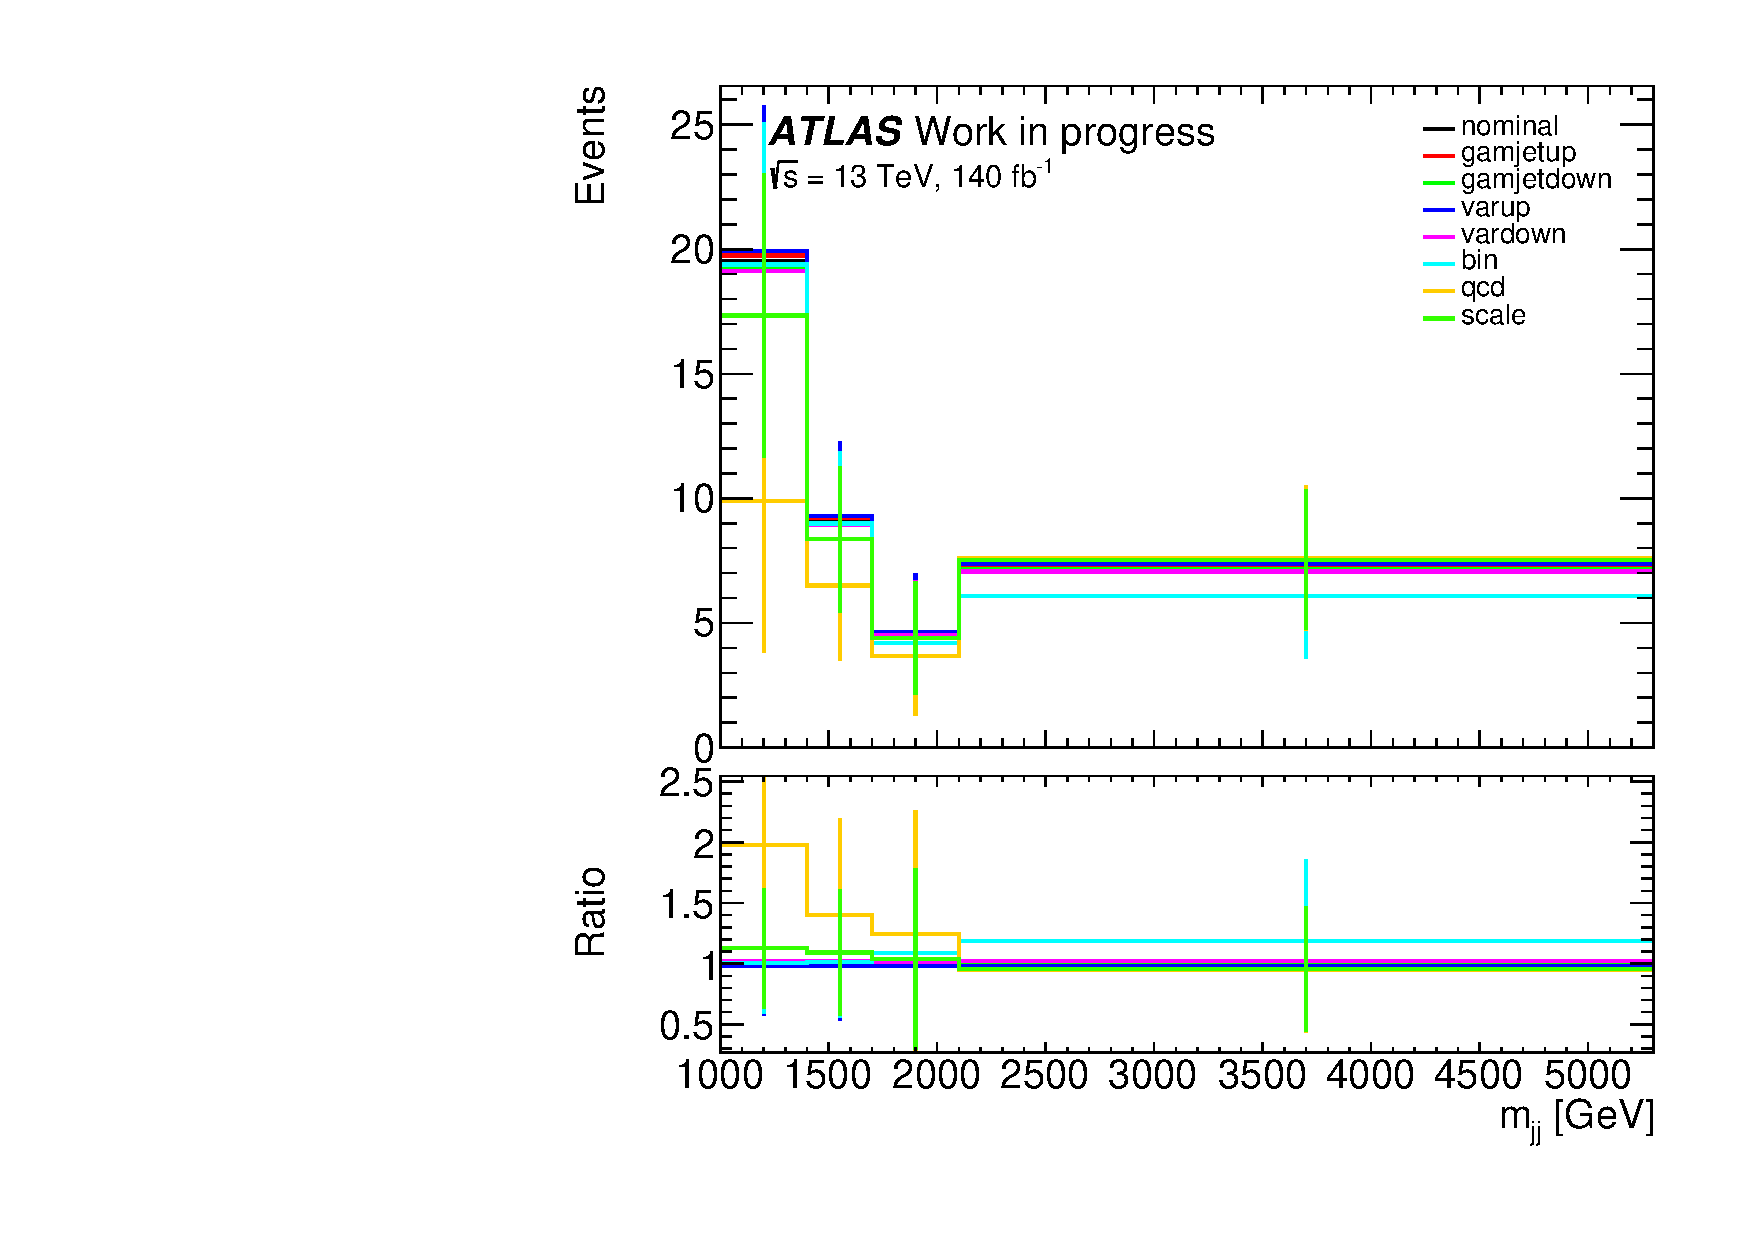
\includegraphics[width=\textwidth]{plots/diffx/ratio_mjj_jfakee.pdf}
    \caption{}
\end{subfigure}
\hfill
\begin{subfigure}[b]{0.48\textwidth}
    \centering
    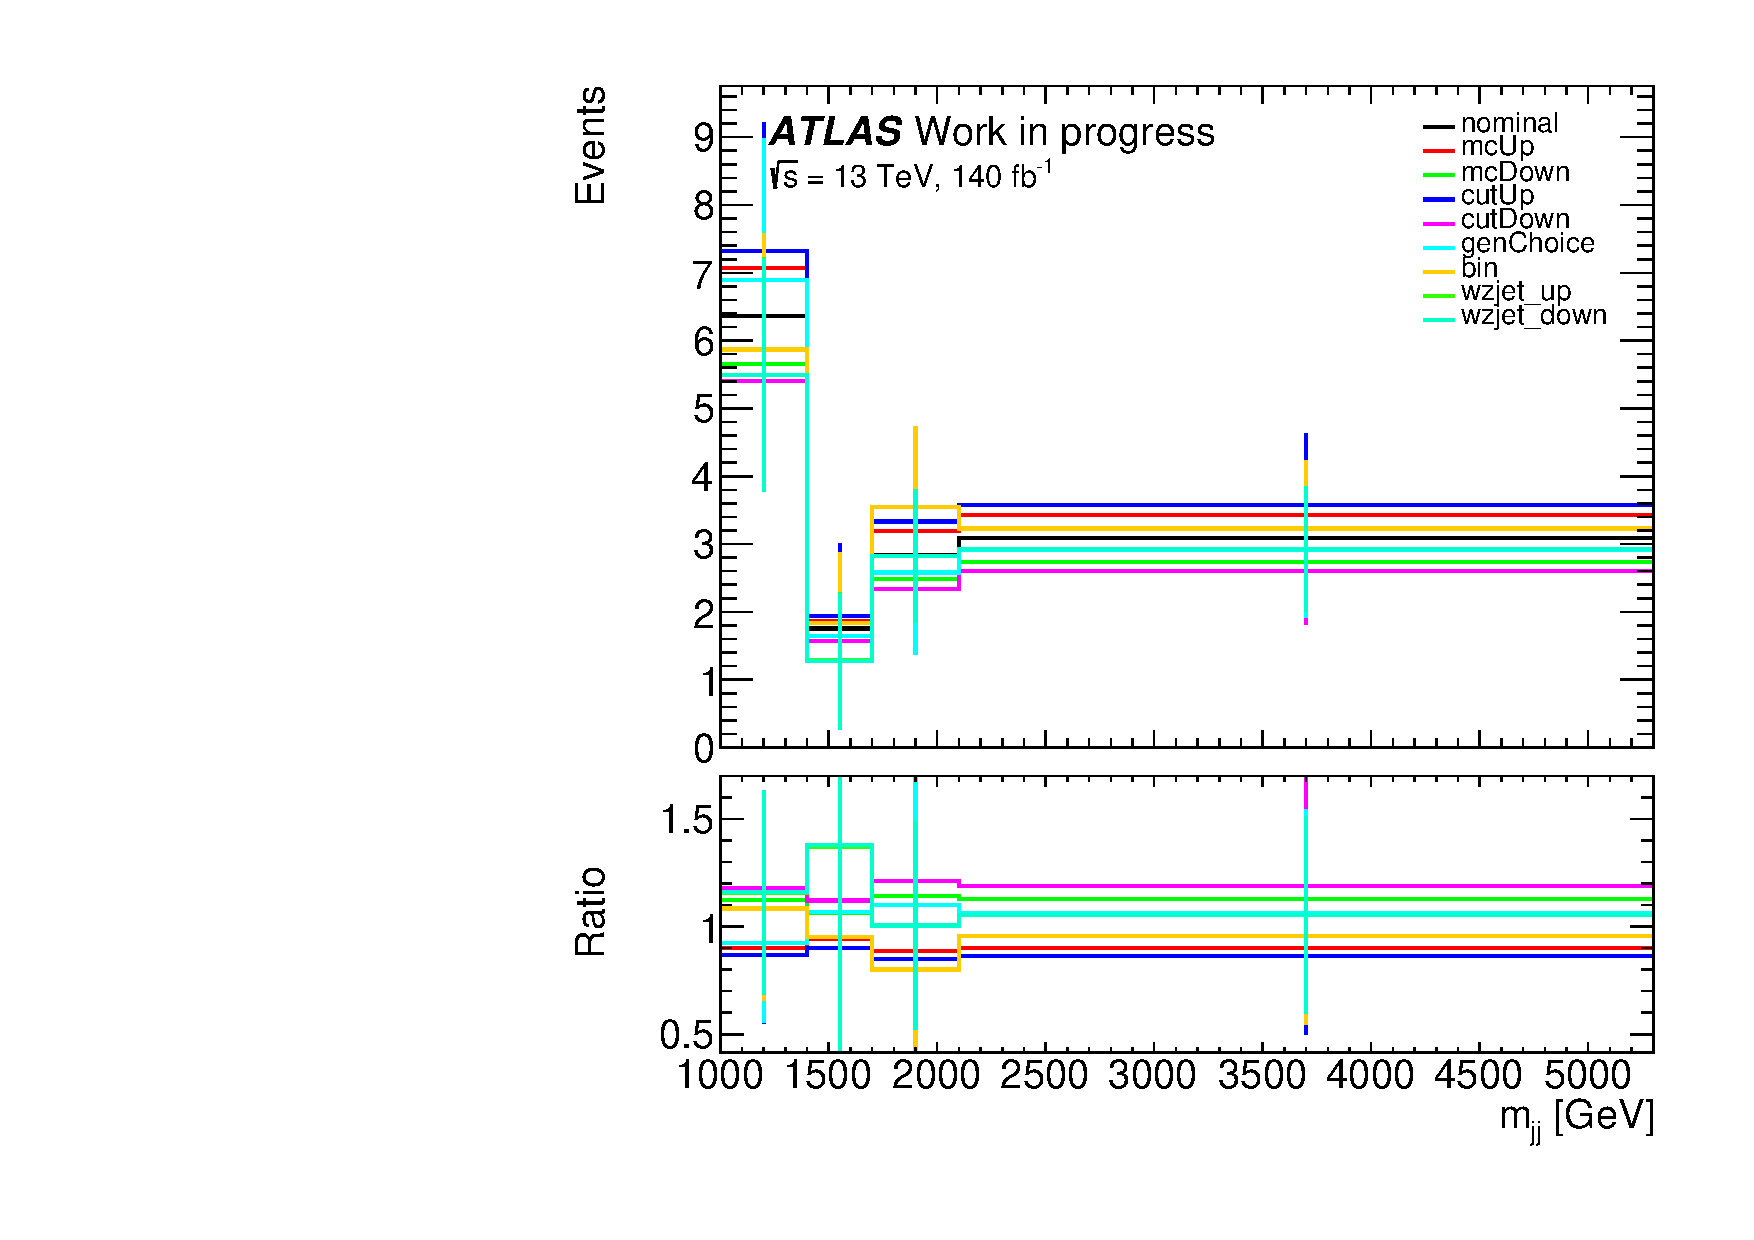
\includegraphics[width=\textwidth]{plots/diffx/ratio_mjj_jfakemu.pdf}
    \caption{}
\end{subfigure}
\caption{Estimates for fake estimate yields with \mjj for \jfakee (a) and \jfakemu (b) in the analysis phase space (no control region cuts). The ratio panel shows the ratio of the systematic variations to the nominal yield. The largest uncertainty comes from variations in the \qcdwy generator choice for \jfakee, and the choice of the dijet sample for \jfakemu. These are shown as ``qcd'' and ``wzjet'' in the legend, respectively. The error bars correspond to statistical uncertainty. Plots made by author from fakes estimates provided by another member of the analysis team.\label{fig:vbswy:jfakel}}
\end{figure}

\subsection{Jets Faking Photons}

The largest background from mis-reconstructed objects comes from jets which are misidentified as photons. This background is estimated using a template fit method, and validated independently using the ABCD method \cite{VBSWy:abcd}. In the template fit method, the fact that the photon isolation energy distribution is different between prompt and non-prompt photons is exploited. First, the photon isolation energy distribution of tight and truth-matched photons in $W\gamma$jj MC samples is used to extract the shape for prompt photons. Next, in a control region populated with mis-reconstructed jets, events in data are used to extract a non-prompt photon isolation energy shape. The control region is defined by one of the non-tight \textit{LoosePrime} photon ID working points described in Section \ref{sec:egamma}. 

For the prompt photon shape, a double-sided crystal ball function\footnote{A crystal ball function \cite{cball1,cball2} is a Gaussian convoluted with a power-law tail. A double-sided crystal ball is the sum of two crystal ball functions sharing the same mean and width.} was found to best describe the photon isolation energy distribution. The fit is performed through maximising the un-binned likelihood over the parameter space given by the free parameters of the function. Similarly, the non-prompt shape is derived through maximising an unbinned likelihood, which is defined by Novosibirsk functions.

To derive the \jfakey estimate, events in data containing a reconstructed tight ID photon are partitioned into bins of the observable for which the estimate is to be derived. For each bin, the prompt and non-prompt functions are combined, and the normalisations of the two functions are derived through maximising a likelihood defined by the products of Novosibirsk and double-sided crystal ball functions. Gaussian constraints defined through the mean and width of the tight and non-tight fits are included in the likelihood to ensure the normalisations do not have unreasonably large deviations from the previously derived values. By integrating the post-fit non-prompt photon isolation energy distribution, the expected number of fake photons is derived.

Systematic uncertainties in the \jfakey estimate arise from statistical uncertainties on the \jfakey yield; from real photon leakage into the LoosePrime control region; from the exact LoosePrime working point; and from MC modelling uncertainties. The nominal and systemic \jfakey yields are shown for \mjj and \ptlep in Figure \ref{fig:vbswy:jfakey}.

\begin{figure}[t]
\centering
\begin{subfigure}[b]{0.48\textwidth}
    \centering
    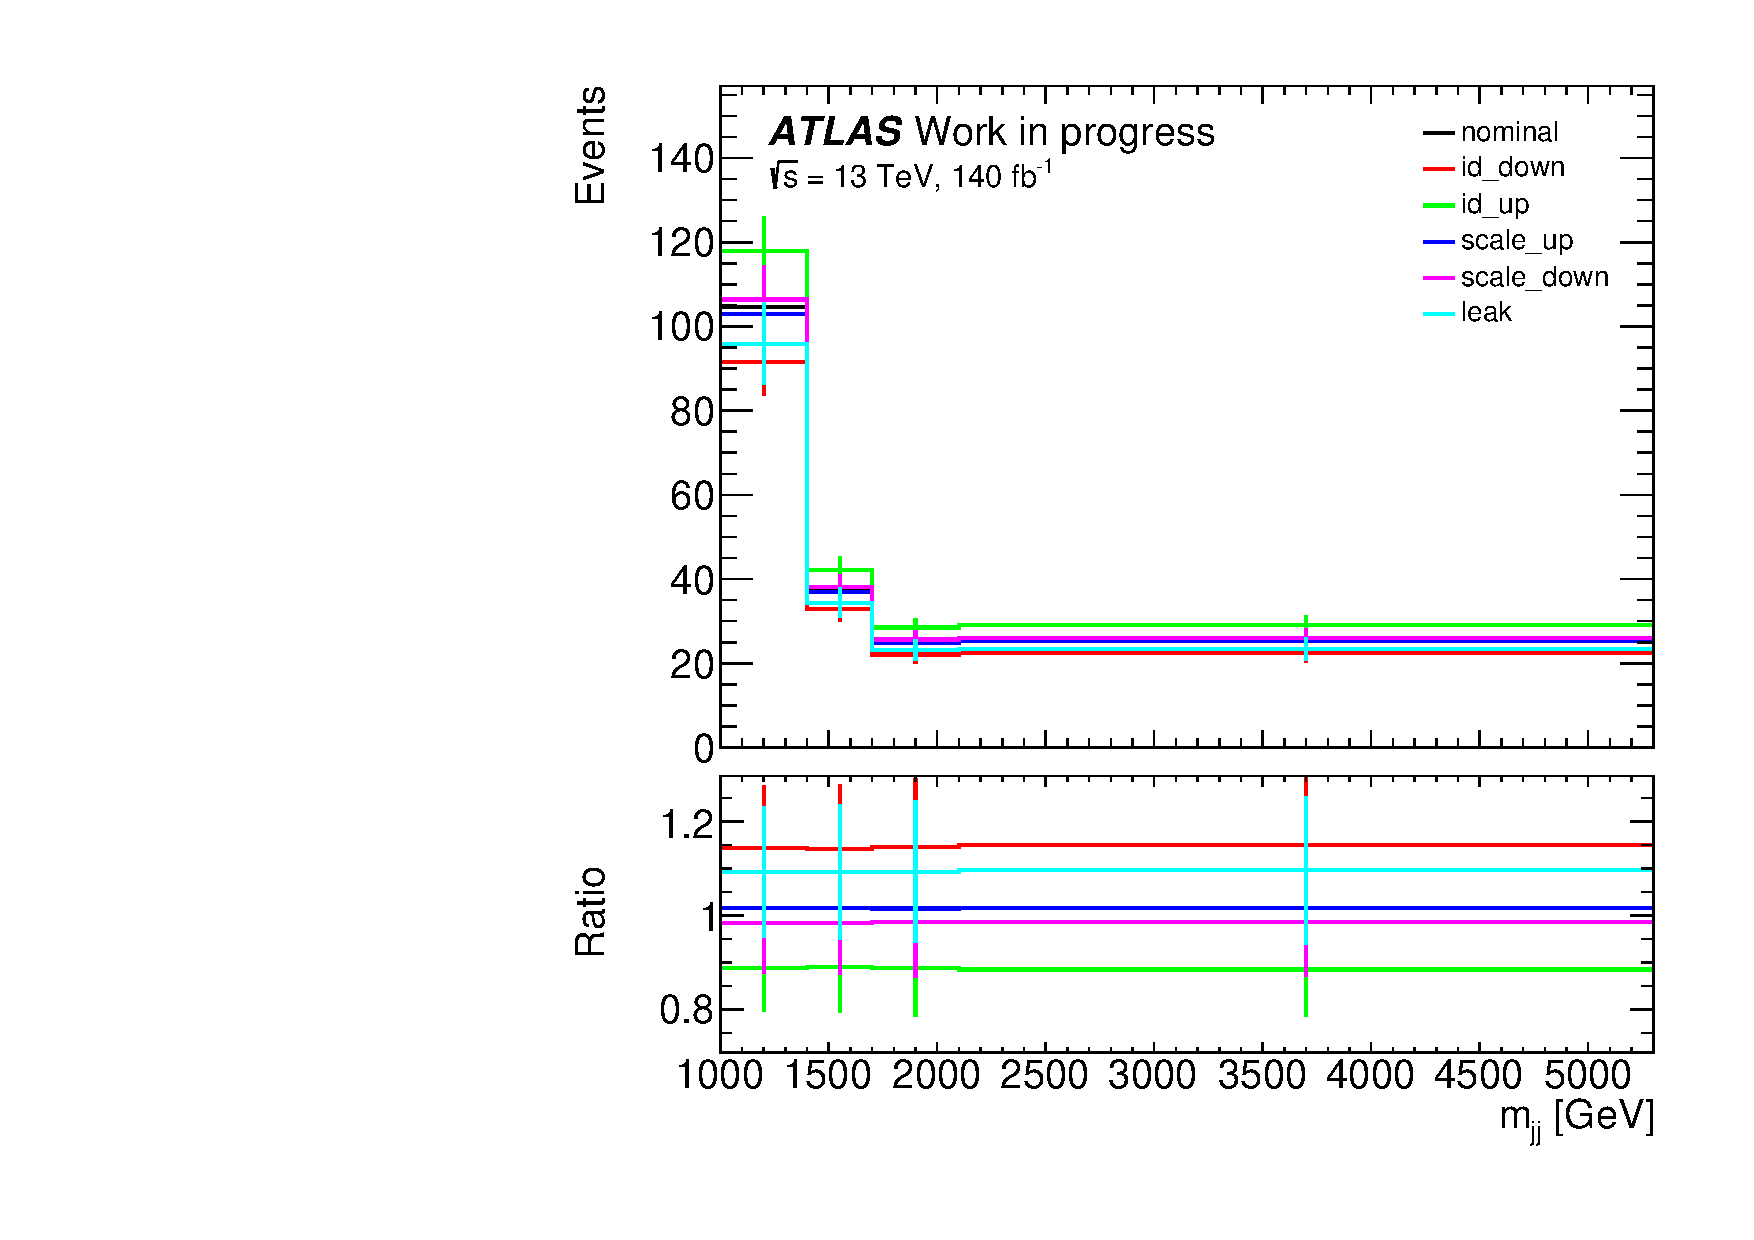
\includegraphics[width=\textwidth]{plots/diffx/ratio_mjj_jfakey.pdf}
    \caption{}
\end{subfigure}
\hfill
\begin{subfigure}[b]{0.48\textwidth}
    \centering
    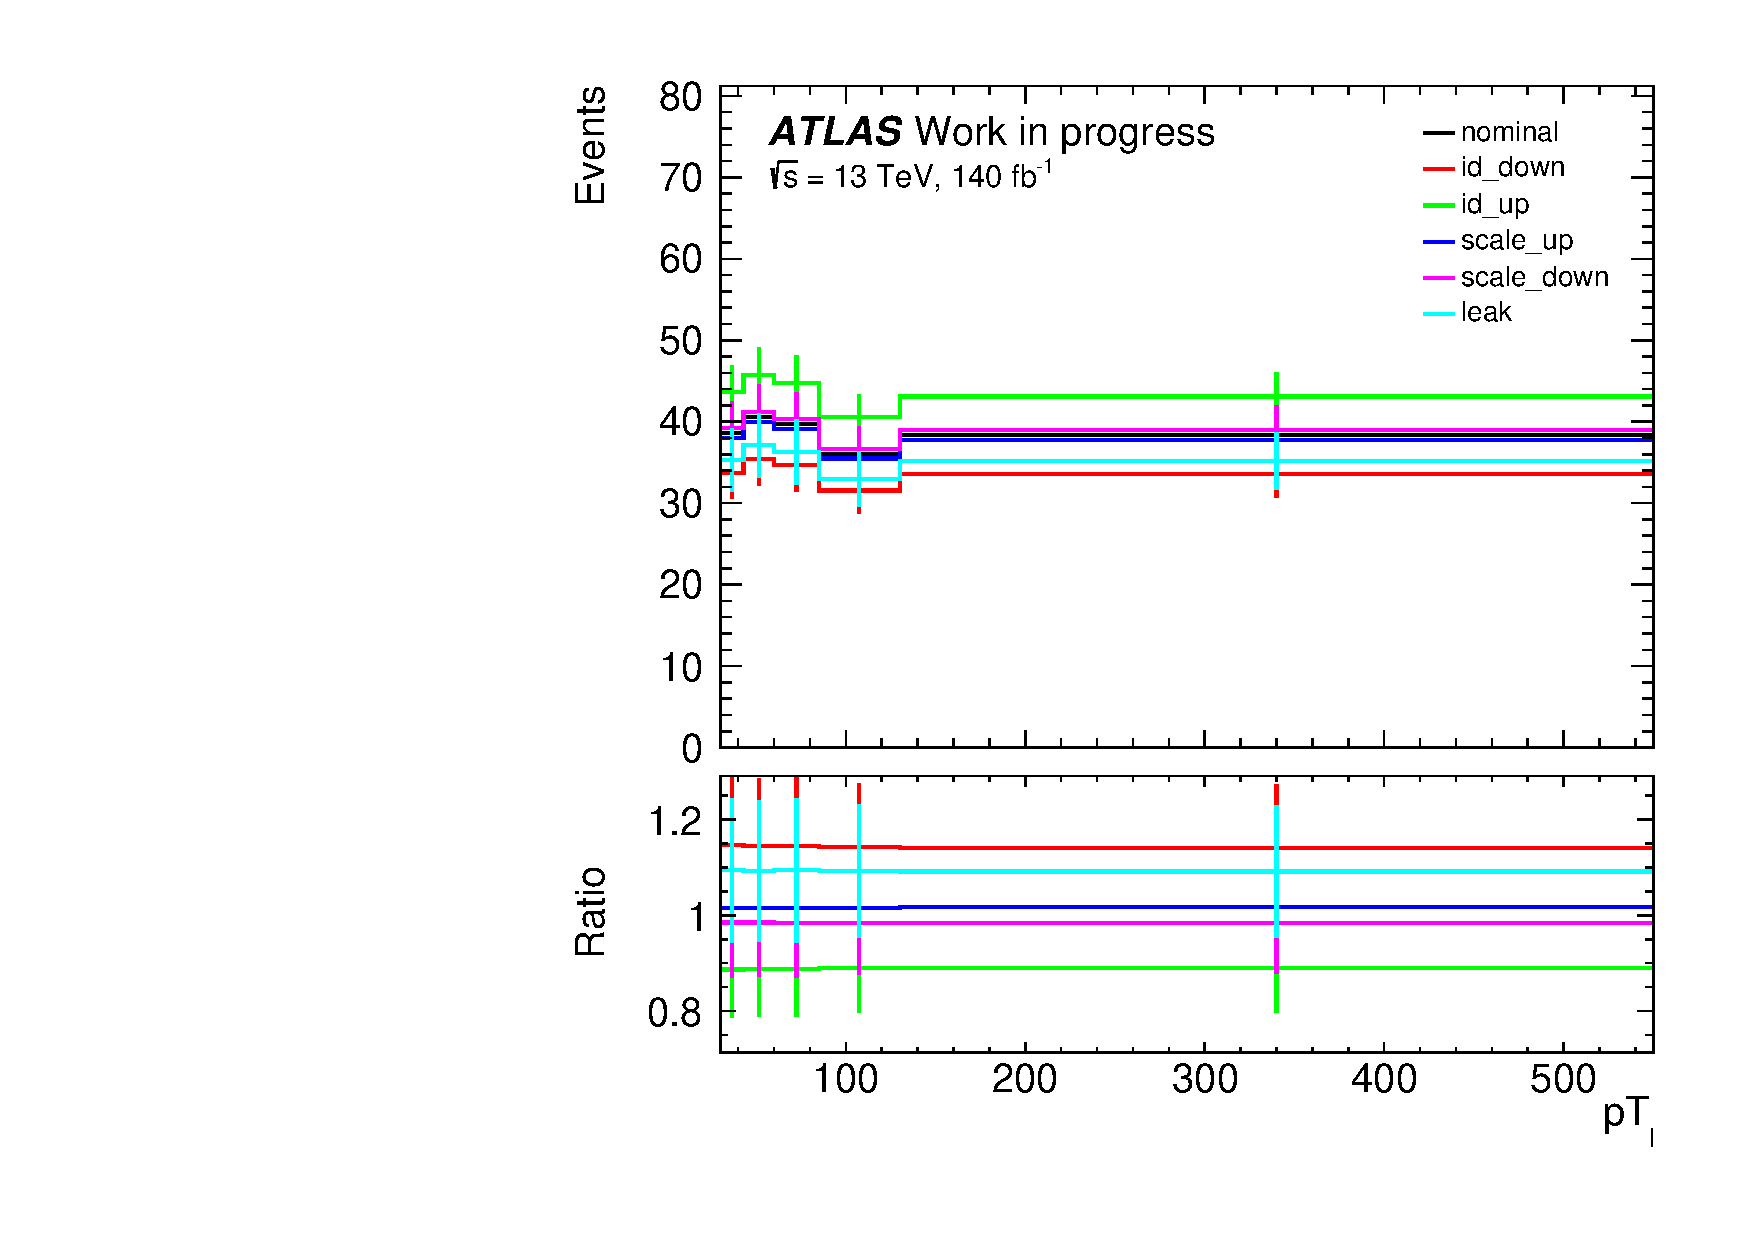
\includegraphics[width=\textwidth]{plots/diffx/ratio_lep_pt_jfakey.pdf}
    \caption{}
\end{subfigure}
%\caption{Estimates for \jfakey yields with \mjj (a) and \leppt (b). The ratio panel shows the ratio of the systematic variations to the nominal yield. The error bars correspond to the statistical uncertainty on the estimate. The error bars are identical for the nominal and systematic yields. The largest uncertainty comes from variations in the LoosePrime definition. These are shown as ``id\tu up'' and ``id\tu down'' in the legend. Plots made by author using fakes estimates not derived by author.\label{fig:vbswy:jfakey}}
\caption{Estimates for \jfakey yields with \mjj (a) and \leppt (b) in the analysis phase space (no control region cuts). The ratio panel shows the ratio of the systematic variations to the nominal yield. The largest uncertainty comes from variations in the LoosePrime definition. These are shown as ``id\tu up'' and ``id\tu down'' in the legend. The error bars correspond to statistical uncertainty. Plots made by author from fakes estimates provided by another member of the analysis team.\label{fig:vbswy:jfakey}}
\end{figure}

\subsection{Electrons Faking Photons}

Prompt electrons and photons leave very similar deposits in the EM calorimeter, i.e. narrow EM showers almost entirely contained in the EM calorimeter. Electrons are distinguished from photons through the presence of a track matched to the primary hard-scatter vertex and the calorimeter deposit. Photons which are converted in the ID can also have an associated track. Electrons can be misidentified as photons primarily due to tracking inefficiencies and bad track-cluster matching.

The \efakey fake rate is measured using the ``tag and probe'' method \cite{VBSWy:tagprobe}. The electron-to-photon fake rate is determined in a control region enriched with $Z\rightarrow ee$ events. A well identified electron is defined as the tag object, and a probe candidate is either a second electron or a photon, where the invariant mass of the tag-probe system corresponds to the $Z$-boson invariant mass. The fake rate is then determined in a similar way to the fake factor method in this $Z\rightarrow ee$ control region. The fake rate is applied in a similar way to equation \ref{eq:fakefactor} to obtain the final \efakey yield. The \efakey yield for \mjj and \leppt in the analysis phase space is shown in Figure \ref{fig:vbswy:efakey}. The \efakey background is validated in the analysis phase space inside of the Z-veto region. 

\begin{figure}[t]
\centering
\begin{subfigure}[b]{0.48\textwidth}
    \centering
    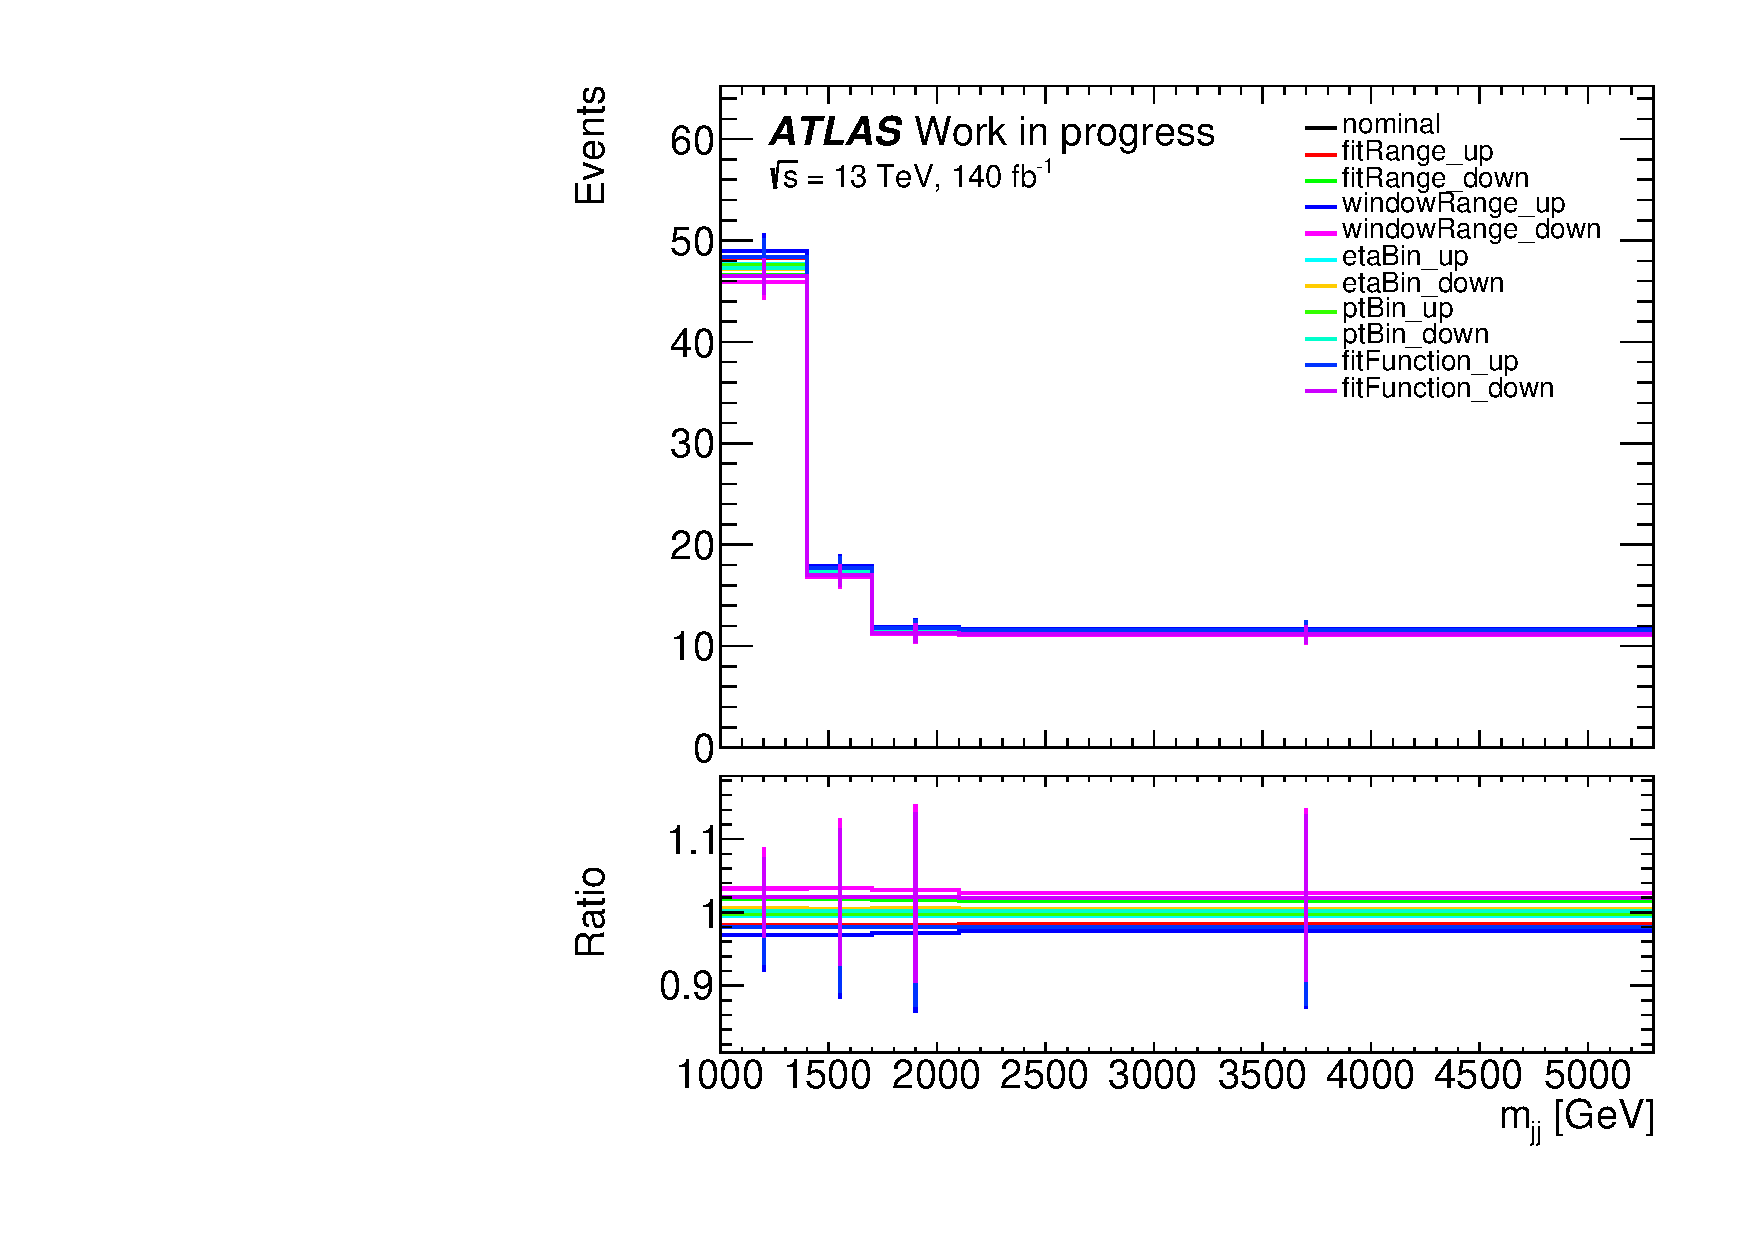
\includegraphics[width=\textwidth]{plots/diffx/ratio_mjj_efakey.pdf}
    \caption{}
\end{subfigure}
\hfill
\begin{subfigure}[b]{0.48\textwidth}
    \centering
    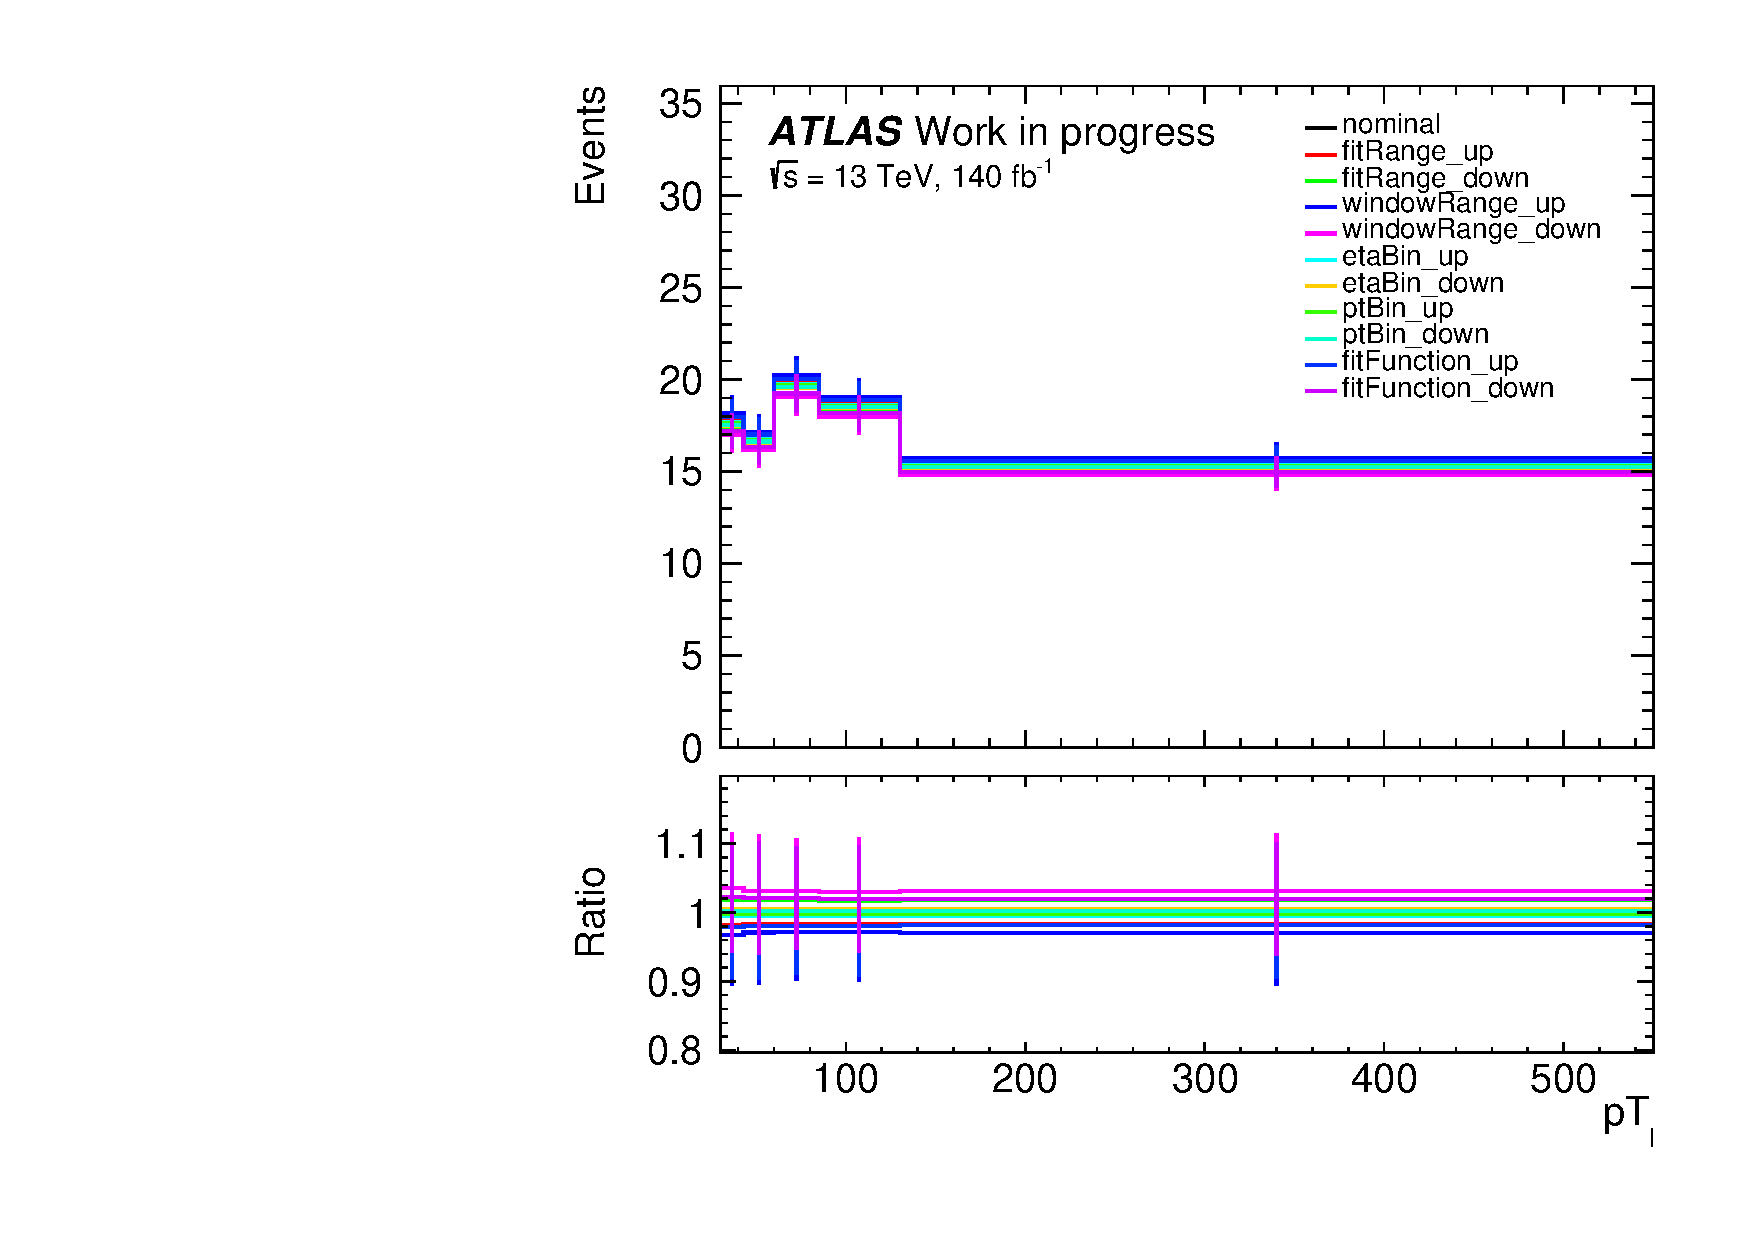
\includegraphics[width=\textwidth]{plots/diffx/ratio_lep_pt_efakey.pdf}
    \caption{}
\end{subfigure}
\caption{Estimates for \efakey yields with \mjj (a) and \leppt (b) in the analysis phase space (no control region cuts). The ratio panel shows the ratio of the systematic variations to the nominal yield. The largest uncertainties come from variations in the function for fitting the signal and background, and the $Z$-mass window range. These are shown as the ``fitFunction'' and ``windowRange'' systematics in the legend. The error bars correspond to statistical uncertainty. Plots made by author from fakes estimates provided by another member of the analysis team.\label{fig:vbswy:efakey}}
\end{figure}

%\clearpage
\section{Expected Yields and Events in Data}

After applying the selection cuts discussed in Section \ref{sec:vbswy:evsel}, the expected event yields from simulation compared with observed numbers of events in data are shown in Figure \ref{fig:vbswy:mcdatayields}. Non-prompt backgrounds are estimated using the methods discussed in the previous section. The agreement between data and prediction is reasonable as a function of \mjj and \jjdphi. However, the data overshoots the prediction at high \mly and low \ptjj.%The agreement between the data and the predictions from simulation are found to agree within about 10\% in most bins, where the maximum disagreement is found to be in the fourth bin of \mly which displays a disagreement greater than 20\%. The distributions for all observables except \mjj and \jjdphi all contain bins with a greater than $2\sigma$ disagreement. If the disagreement between data and simulation is entirely due to statistics, one would expect one or two bins to be separated by more than $2\sigma$ (i.e. $0.05\times5\times6=1.5$ for 5 bins and 6 observables). Therefore these results show that there is some degree of mismodelling of the simulations. From the dijet mass spectrum, the purity of the signal is seen to be highly dependent on \mjj in particular. %For five bins, the expected number of bins with a $>2\sigma$ disagreement is about $0.05*5=0.25$
%The event yields for individual MC samples and data are shown in \Cref{tab:vbswy:yieldsmjj,tab:vbswy:yieldsjjpt,tab:vbswy:yieldsjjdphi,tab:vbswy:yieldsleppt,tab:vbswy:yieldslepgamdphi,tab:vbswy:yieldslym}.
%The uncertainties on the event yields show the MC and data statistical uncertainties. 

\begin{figure}[htpb]
\centering
\begin{subfigure}[b]{0.48\textwidth}
    \centering
    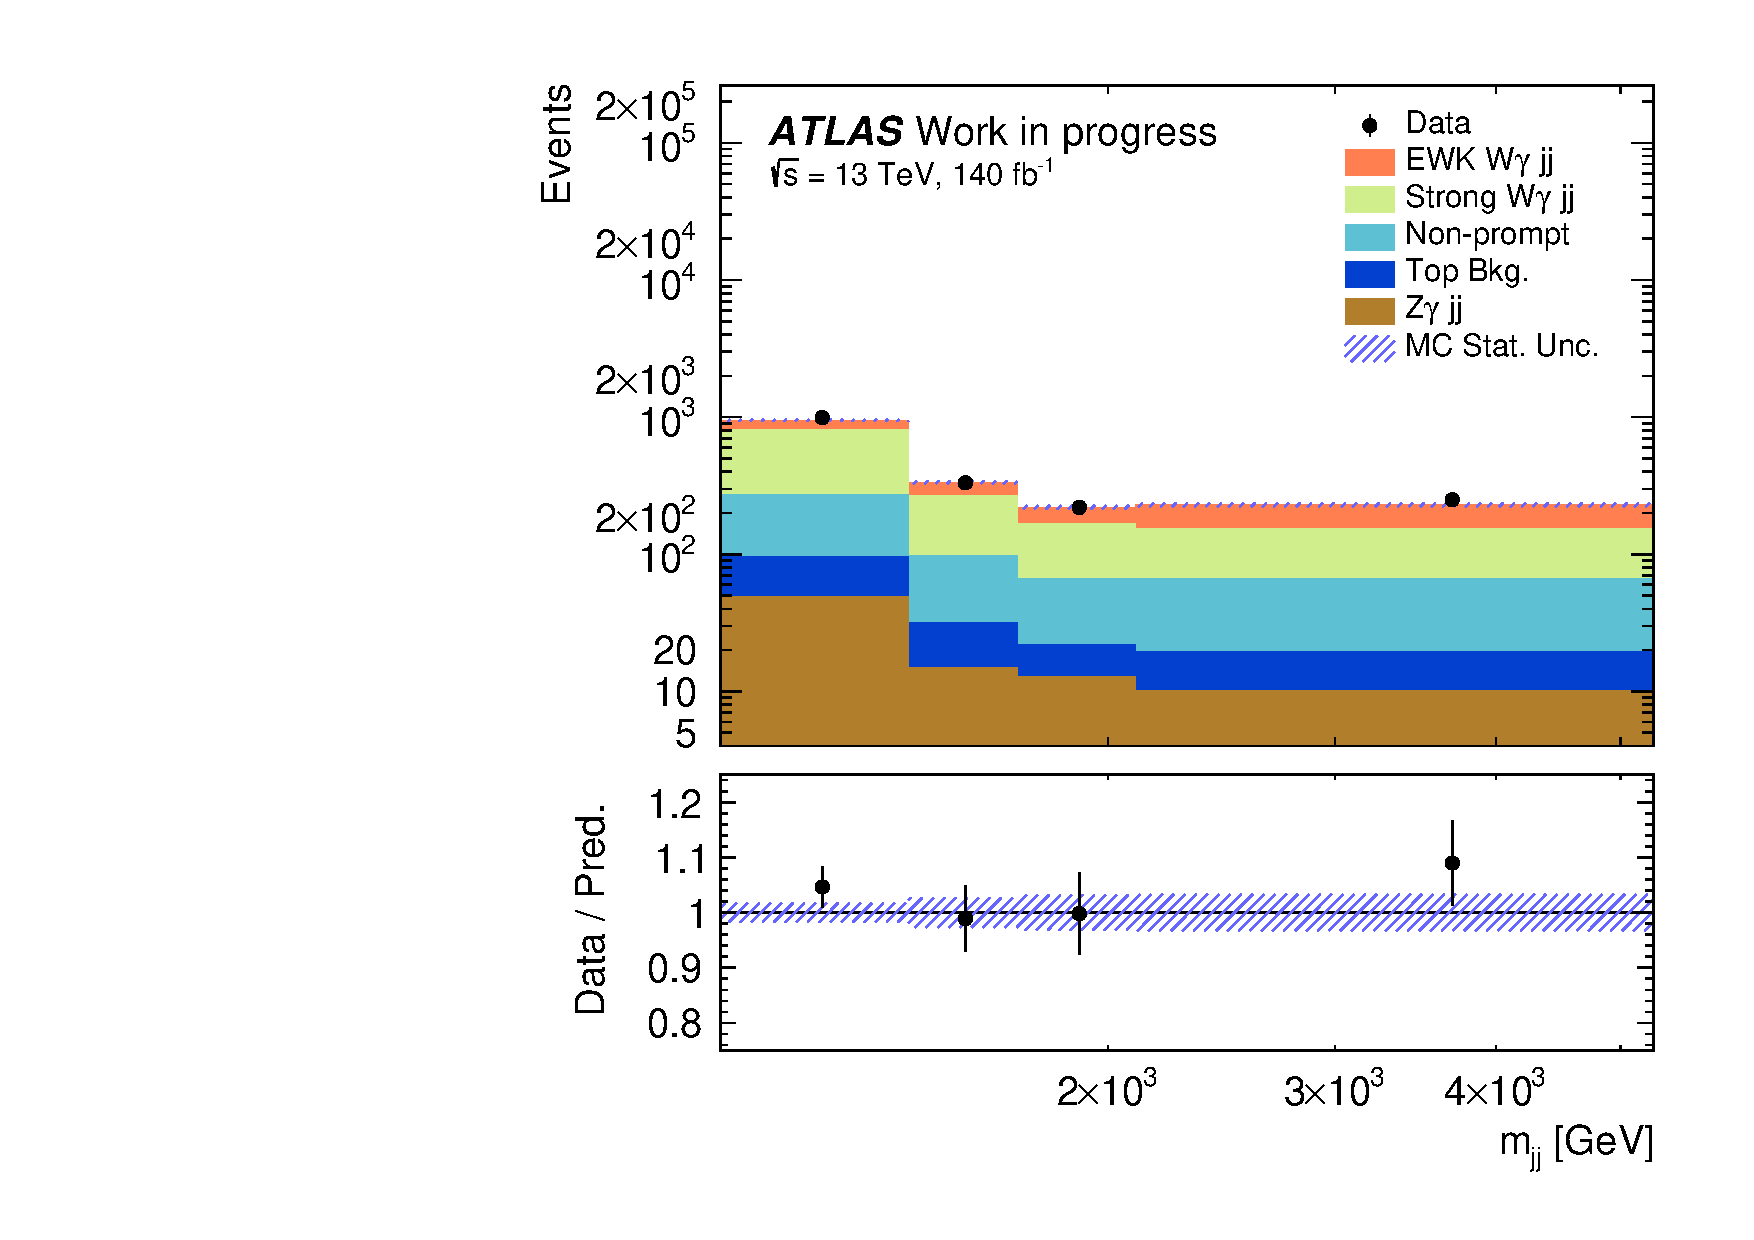
\includegraphics[width=\textwidth]{plots/diffx/combined_stacks/data_vs_mc_mjj.pdf}
    \caption{}
\end{subfigure}
\hfill
\begin{subfigure}[b]{0.48\textwidth}
    \centering
    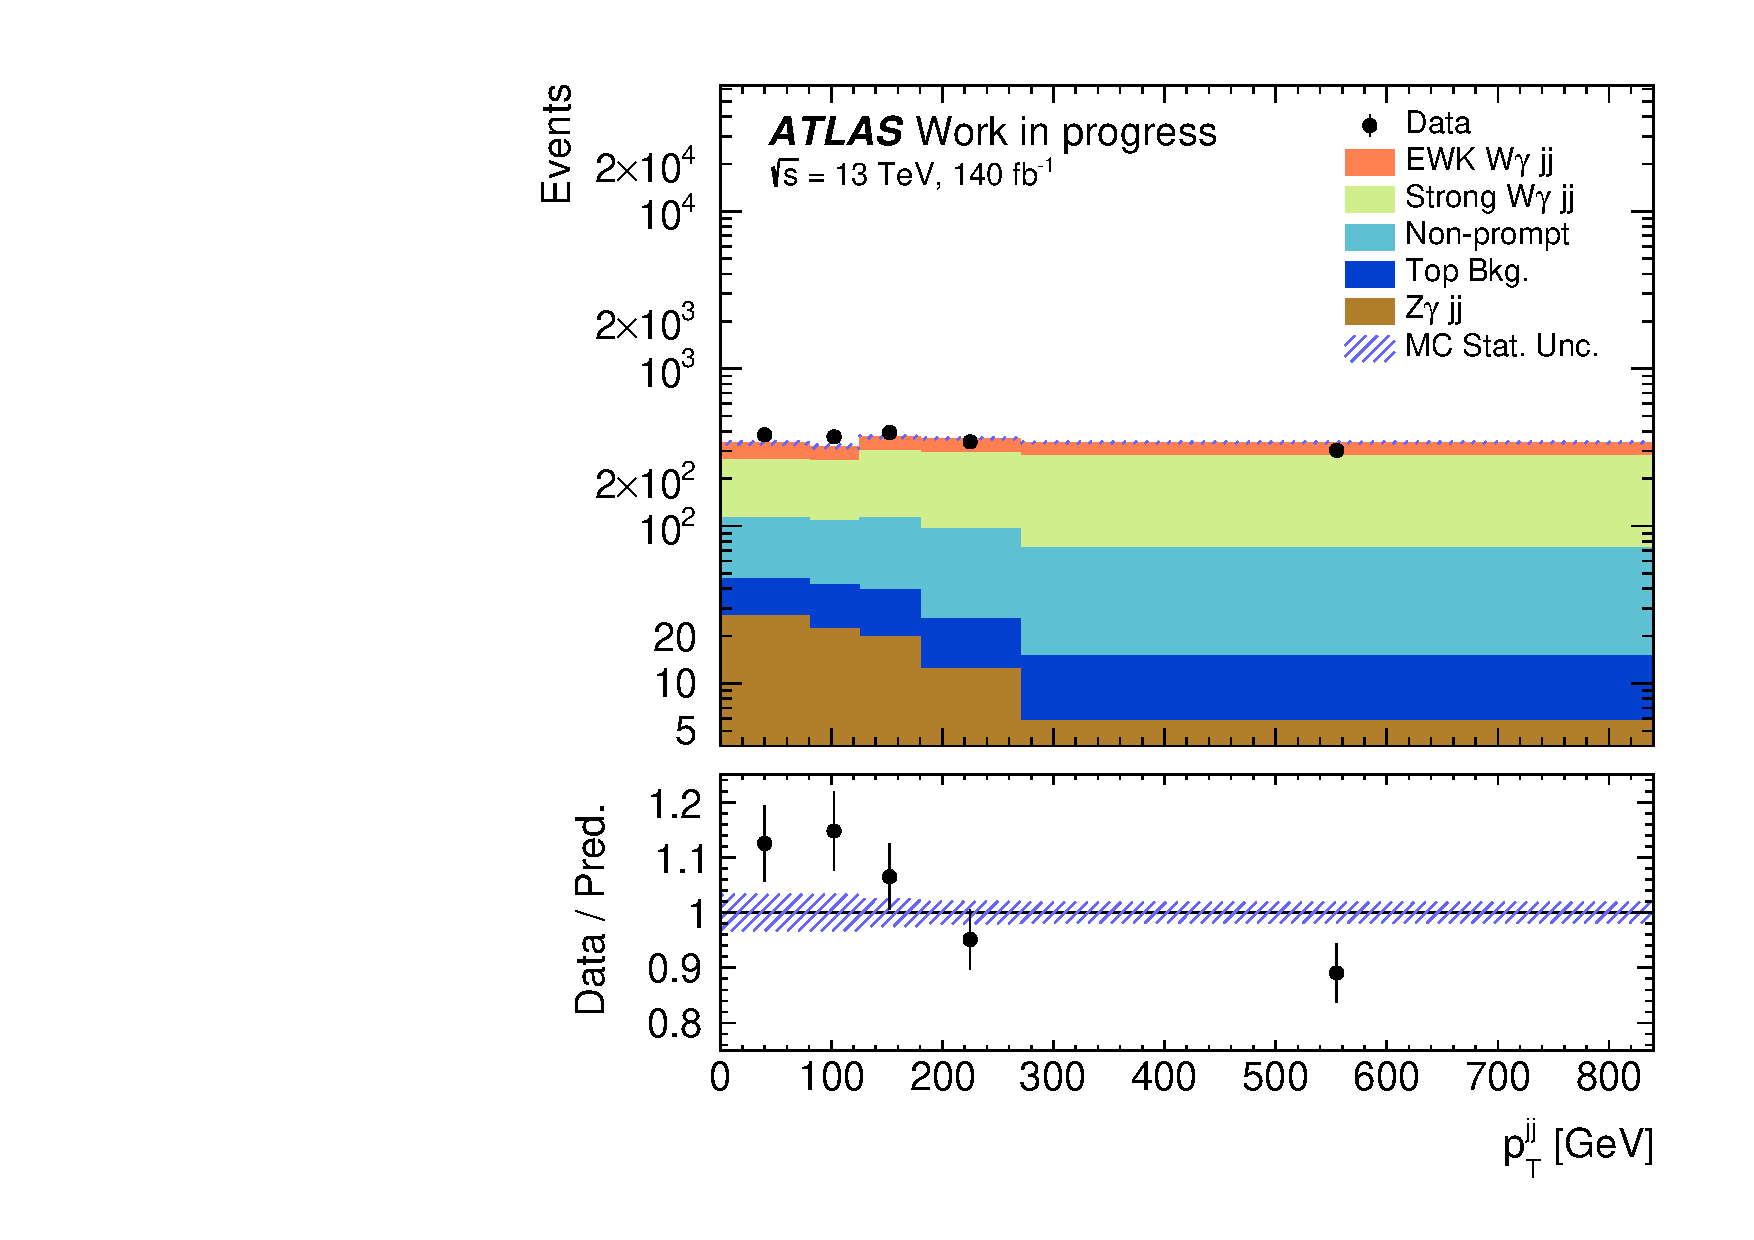
\includegraphics[width=\textwidth]{plots/diffx/combined_stacks/data_vs_mc_jj_pt.pdf}
    \caption{}
\end{subfigure}
\begin{subfigure}[b]{0.48\textwidth}
    \centering
    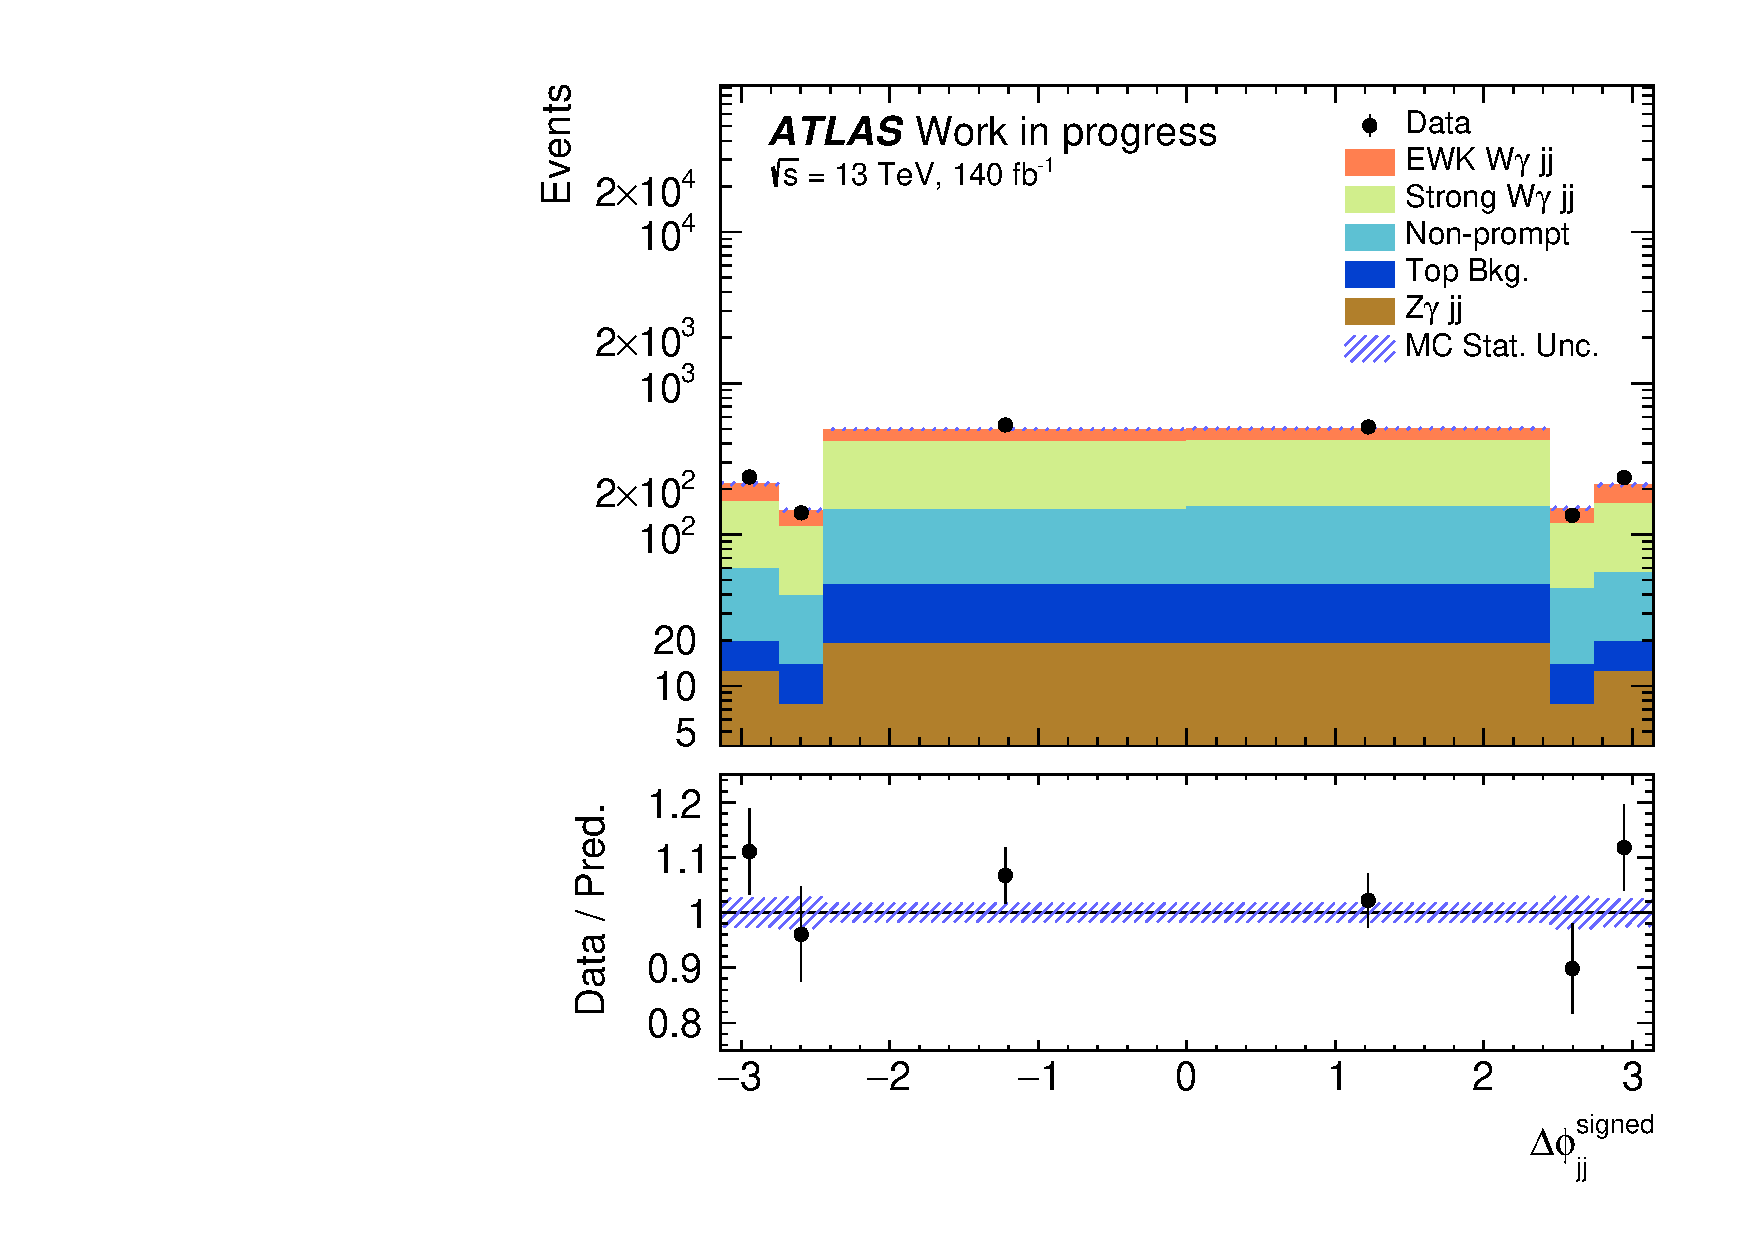
\includegraphics[width=\textwidth]{plots/diffx/combined_stacks/data_vs_mc_jj_dphi.pdf}
    \caption{}
\end{subfigure}
\hfill
\begin{subfigure}[b]{0.48\textwidth}
    \centering
    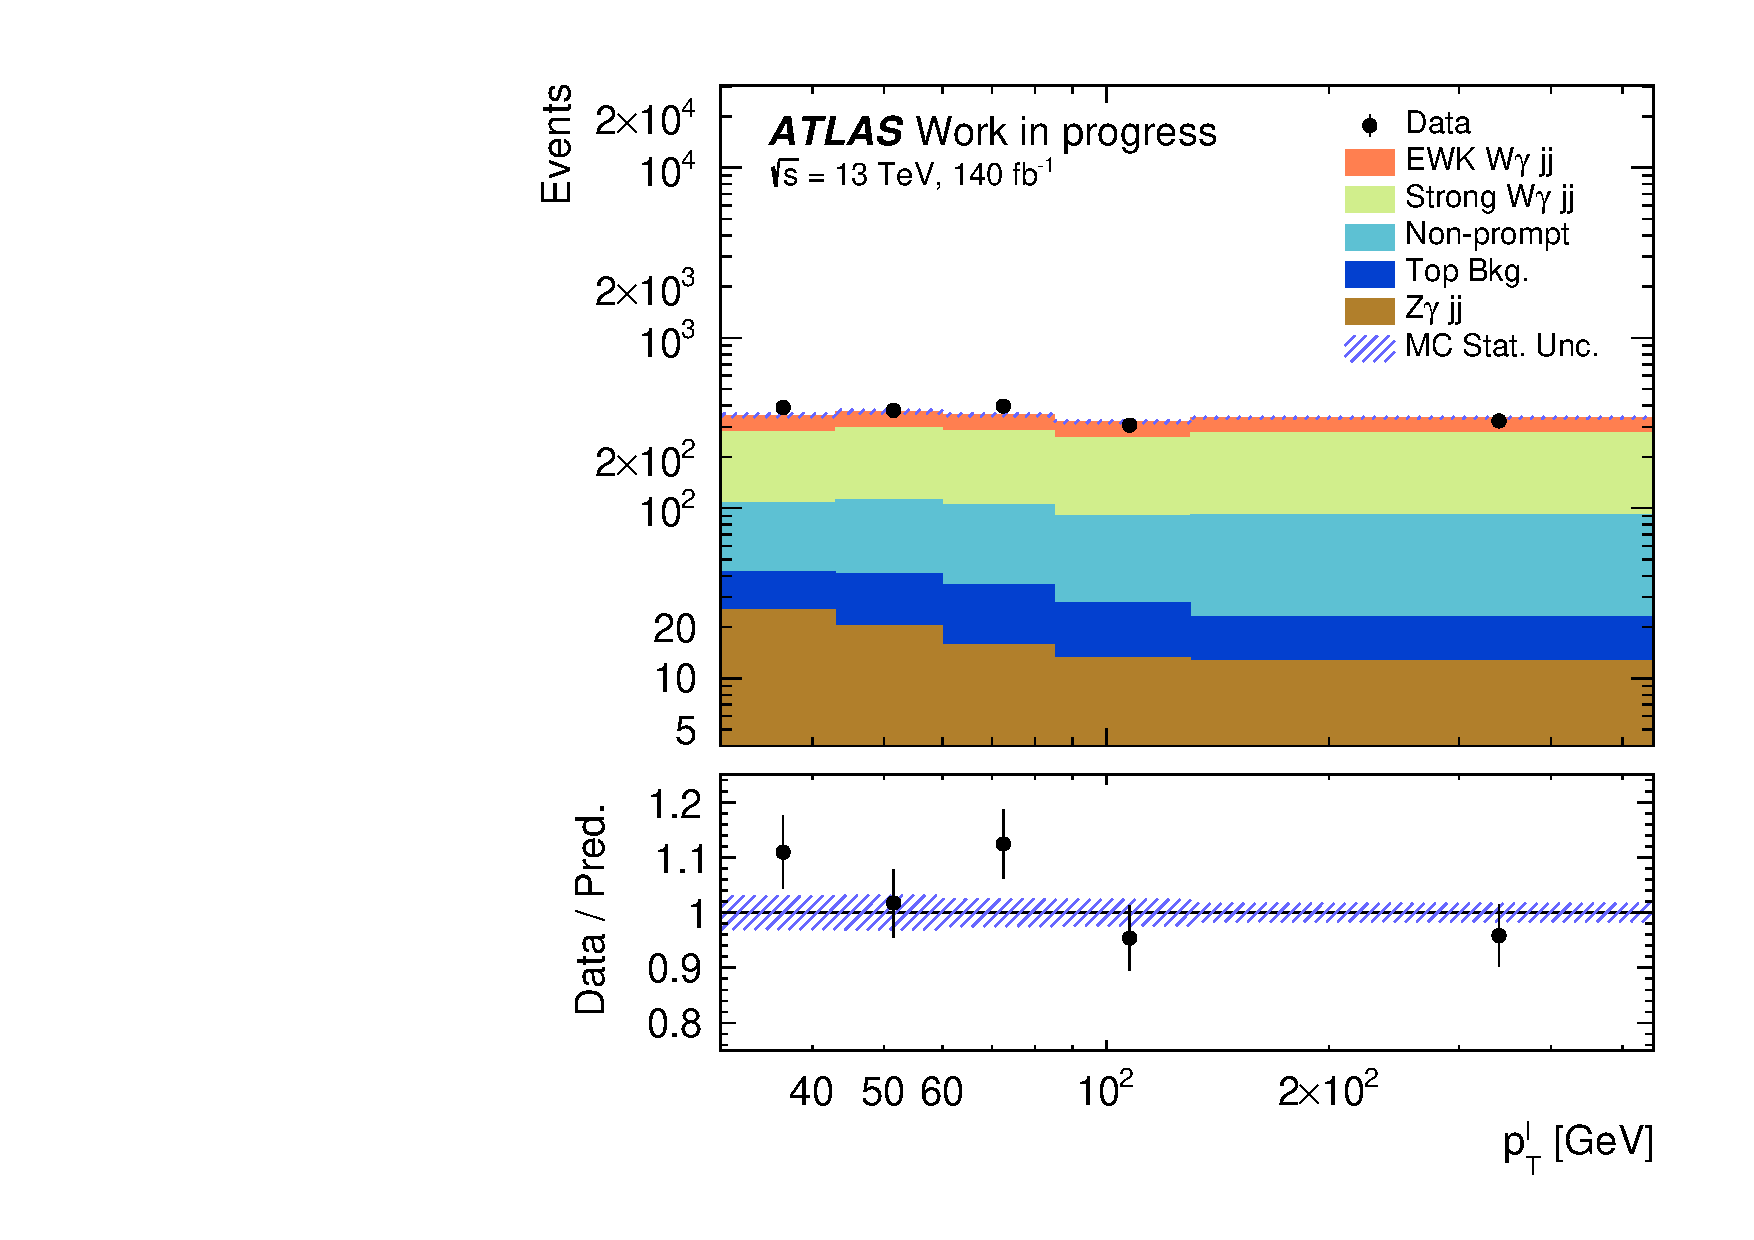
\includegraphics[width=\textwidth]{plots/diffx/combined_stacks/data_vs_mc_lep_pt.pdf}
    \caption{}
\end{subfigure}
\begin{subfigure}[b]{0.48\textwidth}
    \centering
    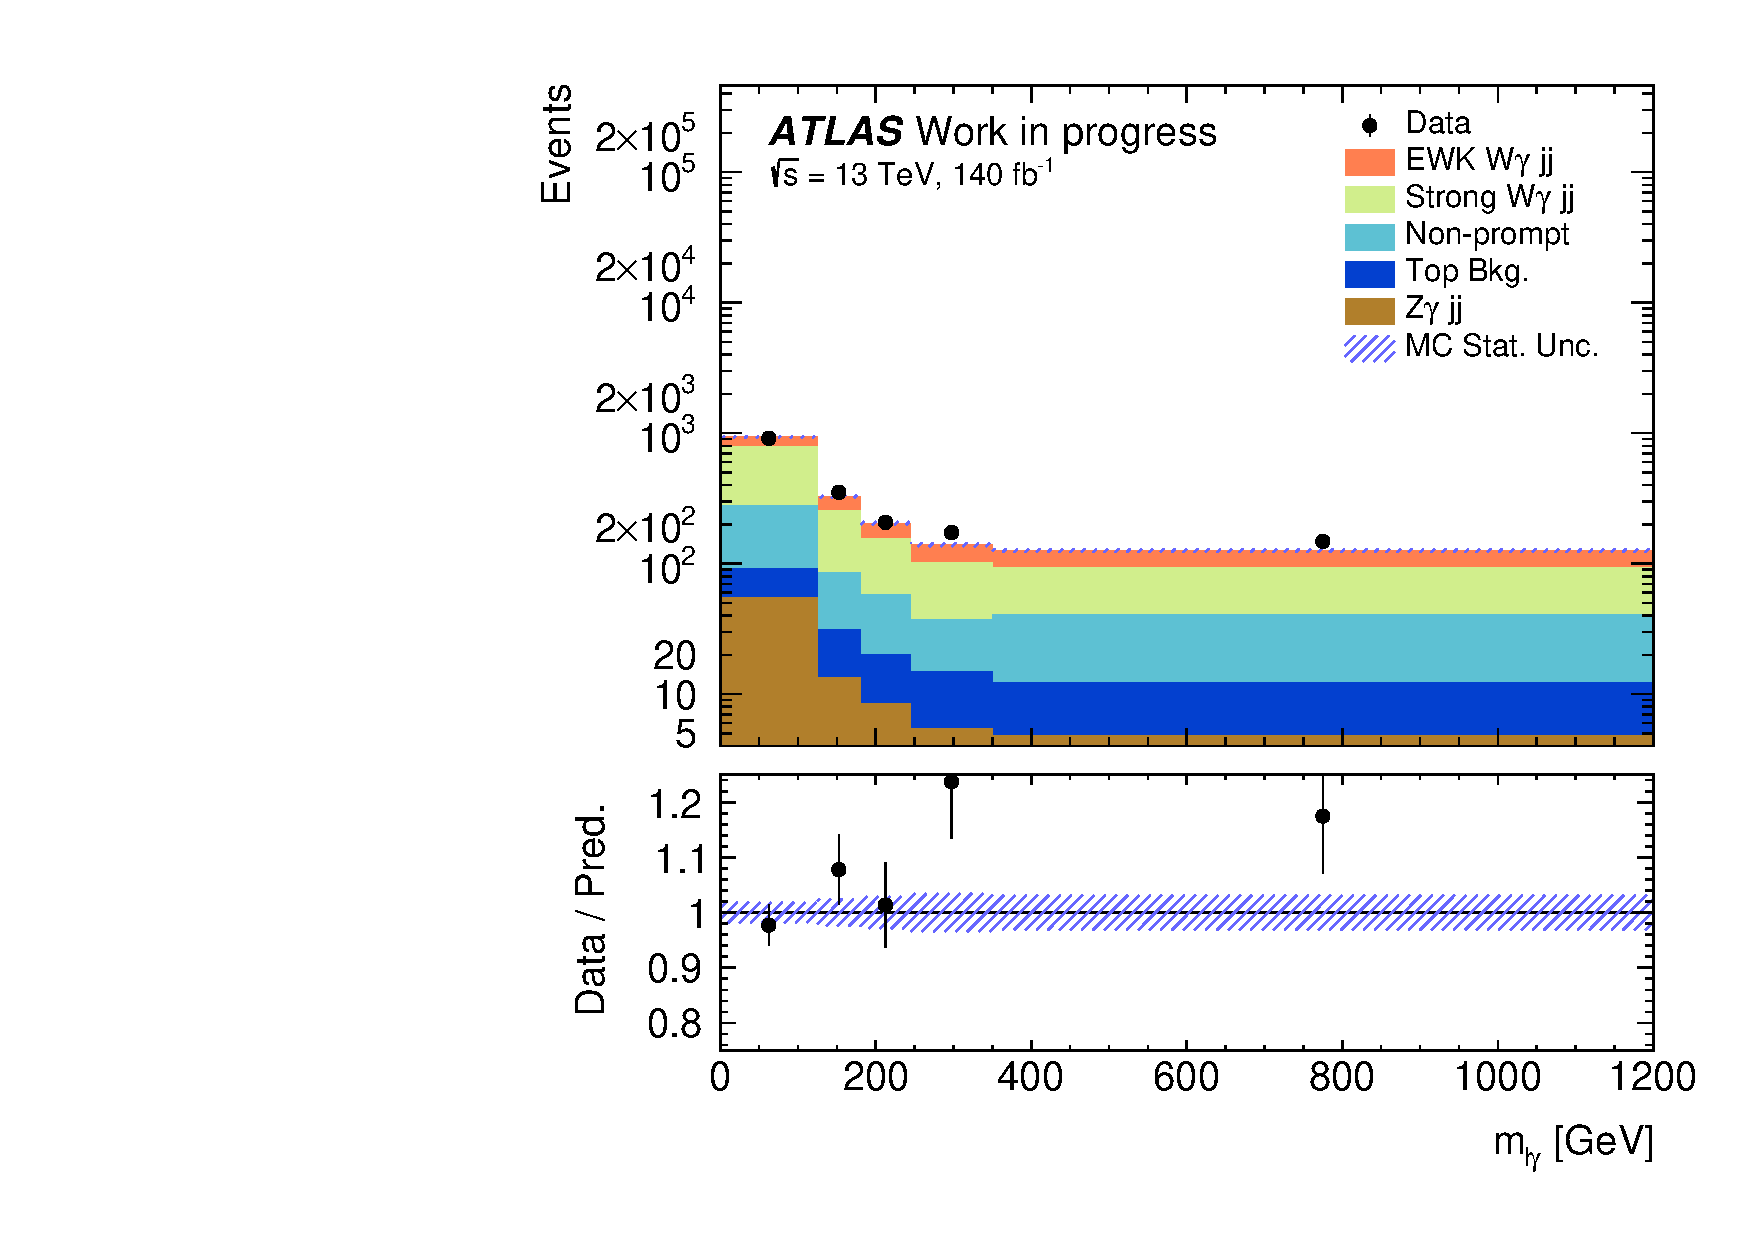
\includegraphics[width=\textwidth]{plots/diffx/combined_stacks/data_vs_mc_ly_m.pdf}
    \caption{}
\end{subfigure}
\hfill
\begin{subfigure}[b]{0.48\textwidth}
    \centering
    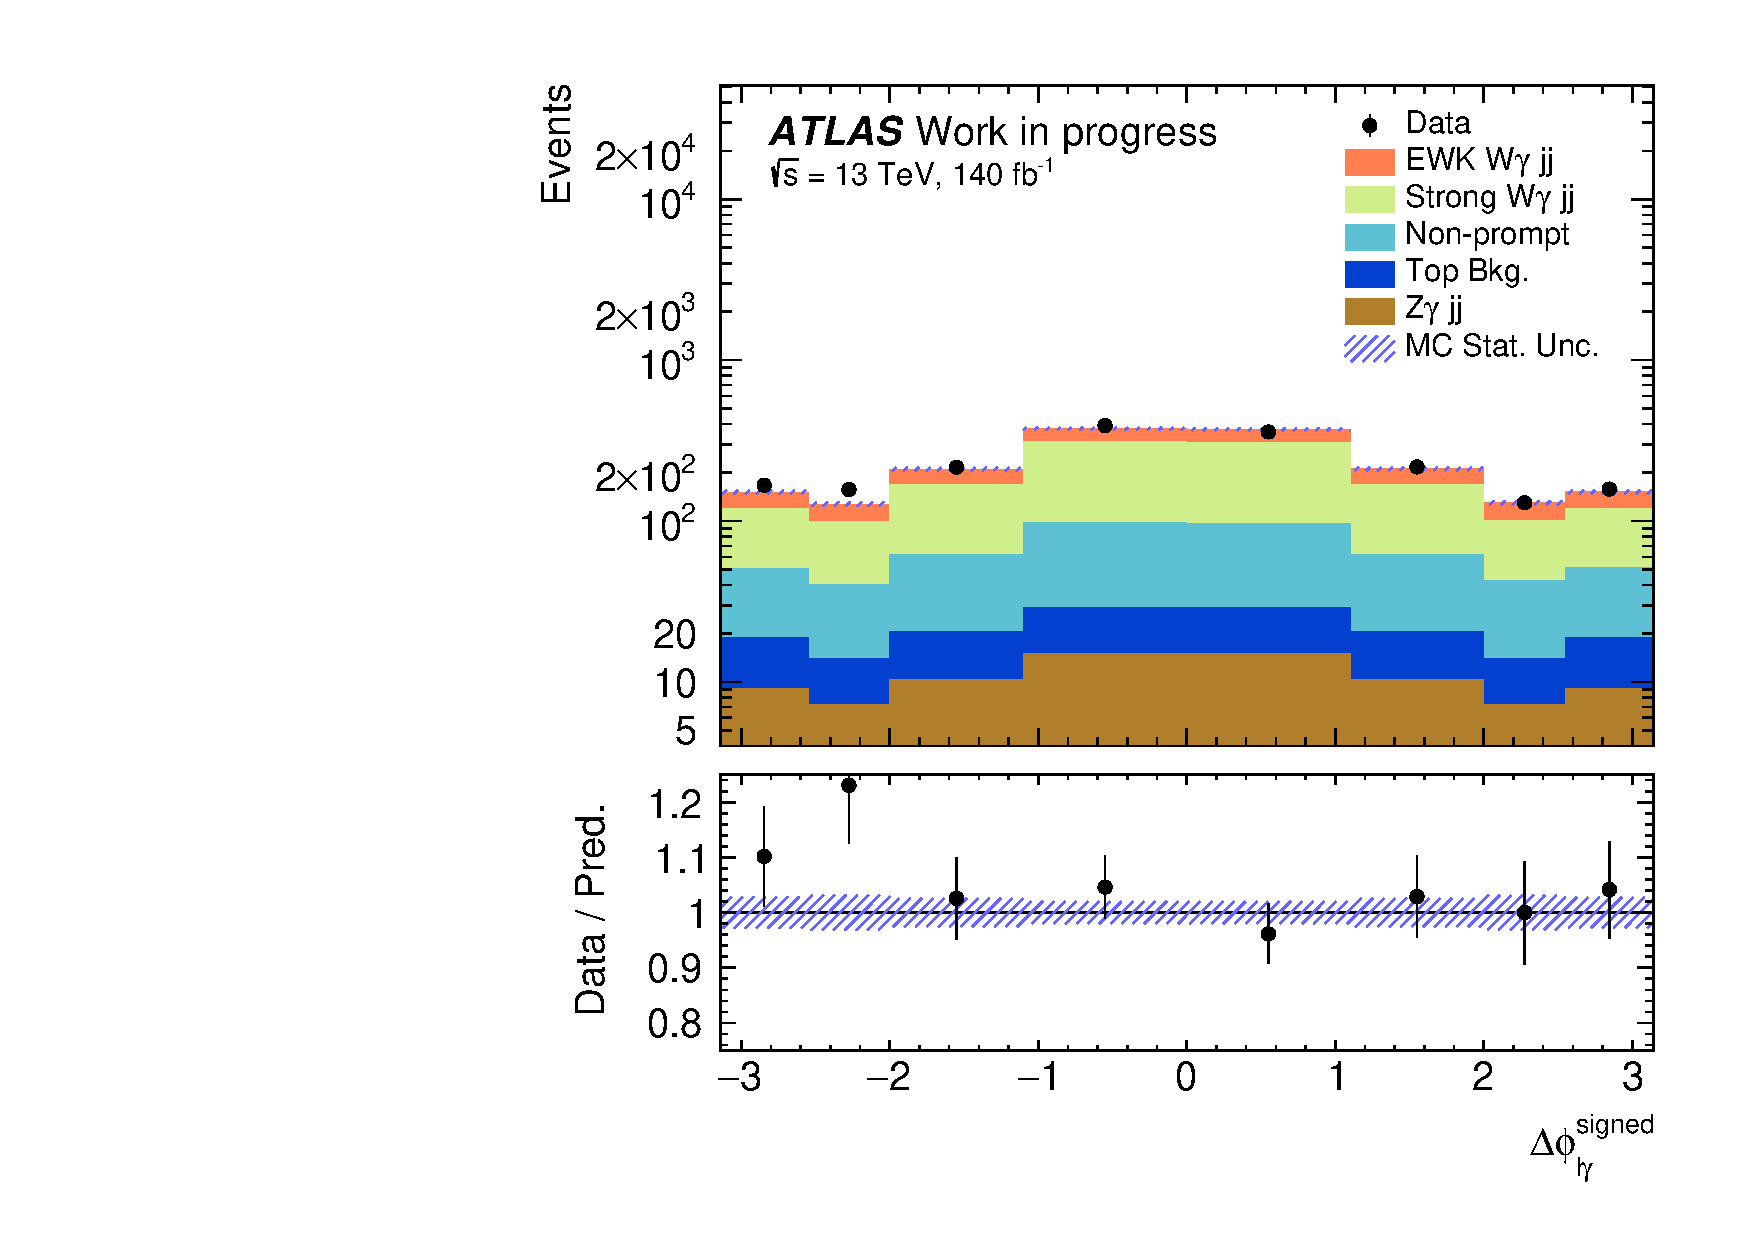
\includegraphics[width=\textwidth]{plots/diffx/combined_stacks/data_vs_mc_lepgam_dphi.pdf}
    \caption{}
\end{subfigure}
\caption{Event yields in the analysis phase space without any control region cuts. The angular observable distributions have been symmetrised. For details on the symmetrisation procedure see Section \ref{sec:vbswy:symdphi}.\label{fig:vbswy:mcdatayields}}
\end{figure}
%
%\begin{table}[t]
%  \begin{minipage}{.5\linewidth}
%    \centering
%    \begin{tabular}{|llrl|}
%      \hline
%       Observable   & Sample             &   Bin & Events           \\
%      \hline
%       \mjj         & Non-prompt         &     1 & $178.0 \pm 10.2$ \\
%       \mjj         & Non-prompt         &     2 & $65.8 \pm 4.4$   \\
%       \mjj         & Non-prompt         &     3 & $44.2 \pm 3.4$   \\
%       \mjj         & Non-prompt         &     4 & $47.4 \pm 3.8$   \\
%       \hline
%       \mjj         & Z$\gamma$jj        &     1 & $49.5 \pm 4.1$   \\
%       \mjj         & Z$\gamma$jj        &     2 & $15.0 \pm 2.3$   \\
%       \mjj         & Z$\gamma$jj        &     3 & $13.0 \pm 2.2$   \\
%       \mjj         & Z$\gamma$jj        &     4 & $10.2 \pm 1.5$   \\
%       \hline
%       \mjj         & Top Bkg.           &     1 & $46.3 \pm 3.3$   \\
%       \mjj         & Top Bkg.           &     2 & $16.9 \pm 2.2$   \\
%       \mjj         & Top Bkg.           &     3 & $9.2 \pm 1.7$    \\
%       \mjj         & Top Bkg.           &     4 & $9.4 \pm 1.7$    \\
%       \hline
%       \mjj         & Strong W$\gamma$jj &     1 & $534.3 \pm 11.5$ \\
%       \mjj         & Strong W$\gamma$jj &     2 & $172.5 \pm 6.9$  \\
%       \mjj         & Strong W$\gamma$jj &     3 & $102.7 \pm 5.3$  \\
%       \mjj         & Strong W$\gamma$jj &     4 & $87.9 \pm 5.9$   \\
%       \hline
%       \mjj         & EWK W$\gamma$jj    &     1 & $140.8 \pm 2.8$  \\
%       \mjj         & EWK W$\gamma$jj    &     2 & $65.5 \pm 1.9$   \\
%       \mjj         & EWK W$\gamma$jj    &     3 & $51.4 \pm 1.7$   \\
%       \mjj         & EWK W$\gamma$jj    &     4 & $74.5 \pm 2.1$   \\
%       \hline
%       \mjj         & Data               &     1 & $993.0 \pm 31.5$ \\
%       \mjj         & Data               &     2 & $332.0 \pm 18.2$ \\
%       \mjj         & Data               &     3 & $220.0 \pm 14.8$ \\
%       \mjj         & Data               &     4 & $250.0 \pm 15.8$ \\
%      \hline
%    \end{tabular}    
%    \caption{\mjj event yields\label{tab:vbswy:yieldsmjj}}
%  \end{minipage}%
%  \begin{minipage}{.5\linewidth}
%    \centering
%    \begin{tabular}{|llrl|}
%      \hline
%       Observable   & Sample             &   Bin & Events           \\
%      \hline
%       \jjpt        & Non-prompt         &     1 & $66.3 \pm 4.5$   \\
%       \jjpt        & Non-prompt         &     2 & $66.2 \pm 5.0$   \\
%       \jjpt        & Non-prompt         &     3 & $74.1 \pm 5.1$   \\
%       \jjpt        & Non-prompt         &     4 & $70.6 \pm 4.8$   \\
%       \jjpt        & Non-prompt         &     5 & $58.1 \pm 4.4$   \\
%       \hline
%       \jjpt        & Z$\gamma$jj        &     1 & $27.1 \pm 3.1$   \\
%       \jjpt        & Z$\gamma$jj        &     2 & $22.5 \pm 3.6$   \\
%       \jjpt        & Z$\gamma$jj        &     3 & $19.9 \pm 2.1$   \\
%       \jjpt        & Z$\gamma$jj        &     4 & $12.4 \pm 1.4$   \\
%       \jjpt        & Z$\gamma$jj        &     5 & $5.8 \pm 0.6$    \\
%       \hline
%       \jjpt        & Top Bkg.           &     1 & $19.6 \pm 2.5$   \\
%       \jjpt        & Top Bkg.           &     2 & $20.0 \pm 2.2$   \\
%       \jjpt        & Top Bkg.           &     3 & $19.5 \pm 2.1$   \\
%       \jjpt        & Top Bkg.           &     4 & $13.6 \pm 2.1$   \\
%       \jjpt        & Top Bkg.           &     5 & $9.2 \pm 1.3$    \\
%       \hline
%       \jjpt        & Strong W$\gamma$jj &     1 & $151.5 \pm 9.3$  \\
%       \jjpt        & Strong W$\gamma$jj &     2 & $152.3 \pm 8.3$  \\
%       \jjpt        & Strong W$\gamma$jj &     3 & $187.3 \pm 6.9$  \\
%       \jjpt        & Strong W$\gamma$jj &     4 & $194.8 \pm 4.6$  \\
%       \jjpt        & Strong W$\gamma$jj &     5 & $206.9 \pm 4.2$  \\
%       \hline
%       \jjpt        & EWK W$\gamma$jj    &     1 & $73.2 \pm 2.1$   \\
%       \jjpt        & EWK W$\gamma$jj    &     2 & $60.4 \pm 1.9$   \\
%       \jjpt        & EWK W$\gamma$jj    &     3 & $68.3 \pm 2.0$   \\
%       \jjpt        & EWK W$\gamma$jj    &     4 & $69.2 \pm 2.0$   \\
%       \jjpt        & EWK W$\gamma$jj    &     5 & $60.2 \pm 1.9$   \\
%       \hline
%       \jjpt        & Data               &     1 & $380.0 \pm 19.5$ \\
%       \jjpt        & Data               &     2 & $369.0 \pm 19.2$ \\
%       \jjpt        & Data               &     3 & $393.0 \pm 19.8$ \\
%       \jjpt        & Data               &     4 & $343.0 \pm 18.5$ \\
%       \jjpt        & Data               &     5 & $303.0 \pm 17.4$ \\
%      \hline
%    \end{tabular}
%    \caption{\jjpt event yields\label{tab:vbswy:yieldsjjpt}}
%  \end{minipage} 
%\end{table}
%
%\begin{table}[t]
%  \begin{minipage}{.5\linewidth}
%    \centering
%    \begin{tabular}{|llrl|}
%      \hline
%       Observable   & Sample             &   Bin & Events           \\
%      \hline
%       \jjdphi      & Non-prompt         &     1 & $39.7 \pm 3.4$   \\
%       \jjdphi      & Non-prompt         &     2 & $25.8 \pm 2.6$   \\
%       \jjdphi      & Non-prompt         &     3 & $100.7 \pm 6.2$  \\
%       \jjdphi      & Non-prompt         &     4 & $107.0 \pm 6.7$  \\
%       \jjdphi      & Non-prompt         &     5 & $30.2 \pm 2.9$   \\
%       \jjdphi      & Non-prompt         &     6 & $36.5 \pm 2.6$   \\
%       \hline
%       \jjdphi      & Z$\gamma$jj        &     1 & $12.5 \pm 1.2$   \\
%       \jjdphi      & Z$\gamma$jj        &     2 & $7.5 \pm 0.8$    \\
%       \jjdphi      & Z$\gamma$jj        &     3 & $19.2 \pm 1.6$   \\
%       \jjdphi      & Z$\gamma$jj        &     4 & $19.2 \pm 1.6$   \\
%       \jjdphi      & Z$\gamma$jj        &     5 & $7.5 \pm 0.8$    \\
%       \jjdphi      & Z$\gamma$jj        &     6 & $12.5 \pm 1.2$   \\
%       \hline
%       \jjdphi      & Top Bkg.           &     1 & $7.0 \pm 1.0$    \\
%       \jjdphi      & Top Bkg.           &     2 & $6.3 \pm 0.9$    \\
%       \jjdphi      & Top Bkg.           &     3 & $27.6 \pm 1.9$   \\
%       \jjdphi      & Top Bkg.           &     4 & $27.6 \pm 1.9$   \\
%       \jjdphi      & Top Bkg.           &     5 & $6.3 \pm 0.9$    \\
%       \jjdphi      & Top Bkg.           &     6 & $7.0 \pm 1.0$    \\
%       \hline
%       \jjdphi      & Strong W$\gamma$jj &     1 & $105.6 \pm 4.3$  \\
%       \jjdphi      & Strong W$\gamma$jj &     2 & $73.6 \pm 2.9$   \\
%       \jjdphi      & Strong W$\gamma$jj &     3 & $265.9 \pm 5.3$  \\
%       \jjdphi      & Strong W$\gamma$jj &     4 & $265.9 \pm 5.3$  \\
%       \jjdphi      & Strong W$\gamma$jj &     5 & $73.6 \pm 2.9$   \\
%       \jjdphi      & Strong W$\gamma$jj &     6 & $105.6 \pm 4.3$  \\
%       \hline
%       \jjdphi      & EWK W$\gamma$jj    &     1 & $51.3 \pm 1.2$   \\
%       \jjdphi      & EWK W$\gamma$jj    &     2 & $31.5 \pm 1.0$   \\
%       \jjdphi      & EWK W$\gamma$jj    &     3 & $83.2 \pm 1.5$   \\
%       \jjdphi      & EWK W$\gamma$jj    &     4 & $83.2 \pm 1.5$   \\
%       \jjdphi      & EWK W$\gamma$jj    &     5 & $31.5 \pm 1.0$   \\
%       \jjdphi      & EWK W$\gamma$jj    &     6 & $51.3 \pm 1.2$   \\
%       \hline
%       \jjdphi      & Data               &     1 & $240.0 \pm 15.5$ \\
%       \jjdphi      & Data               &     2 & $139.0 \pm 11.8$ \\
%       \jjdphi      & Data               &     3 & $530.0 \pm 23.0$ \\
%       \jjdphi      & Data               &     4 & $514.0 \pm 22.7$ \\
%       \jjdphi      & Data               &     5 & $134.0 \pm 11.6$ \\
%       \jjdphi      & Data               &     6 & $238.0 \pm 15.4$ \\
%      \hline
%    \end{tabular}
%    \caption{\jjdphi event yields\label{tab:vbswy:yieldsjjdphi}}
%  \end{minipage}%
%  \begin{minipage}{.5\linewidth}
%    \centering
%    \begin{tabular}{|llrl|}
%      \hline
%        Observable   & Sample             &   Bin & Events           \\
%      \hline
%        \leppt       & Non-prompt         &     1 & $65.3 \pm 4.4$   \\
%        \leppt       & Non-prompt         &     2 & $71.5 \pm 5.5$   \\
%        \leppt       & Non-prompt         &     3 & $69.7 \pm 5.1$   \\
%        \leppt       & Non-prompt         &     4 & $62.8 \pm 4.5$   \\
%        \leppt       & Non-prompt         &     5 & $69.1 \pm 3.9$   \\
%        \hline
%        \leppt       & Z$\gamma$jj        &     1 & $25.5 \pm 3.4$   \\
%        \leppt       & Z$\gamma$jj        &     2 & $20.5 \pm 3.1$   \\
%        \leppt       & Z$\gamma$jj        &     3 & $15.7 \pm 1.9$   \\
%        \leppt       & Z$\gamma$jj        &     4 & $13.3 \pm 1.8$   \\
%        \leppt       & Z$\gamma$jj        &     5 & $12.6 \pm 1.0$   \\
%        \hline
%        \leppt       & Top Bkg.           &     1 & $16.7 \pm 2.4$   \\
%        \leppt       & Top Bkg.           &     2 & $20.6 \pm 2.5$   \\
%        \leppt       & Top Bkg.           &     3 & $19.9 \pm 2.3$   \\
%        \leppt       & Top Bkg.           &     4 & $14.6 \pm 1.8$   \\
%        \leppt       & Top Bkg.           &     5 & $10.4 \pm 1.1$   \\
%        \hline
%        \leppt       & Strong W$\gamma$jj &     1 & $175.4 \pm 8.7$  \\
%        \leppt       & Strong W$\gamma$jj &     2 & $185.0 \pm 9.3$  \\
%        \leppt       & Strong W$\gamma$jj &     3 & $180.9 \pm 6.4$  \\
%        \leppt       & Strong W$\gamma$jj &     4 & $168.0 \pm 5.5$  \\
%        \leppt       & Strong W$\gamma$jj &     5 & $185.4 \pm 3.4$  \\
%        \hline
%        \leppt       & EWK W$\gamma$jj    &     1 & $68.7 \pm 2.0$   \\
%        \leppt       & EWK W$\gamma$jj    &     2 & $71.1 \pm 2.0$   \\
%        \leppt       & EWK W$\gamma$jj    &     3 & $66.9 \pm 2.0$   \\
%        \leppt       & EWK W$\gamma$jj    &     4 & $63.3 \pm 1.9$   \\
%        \leppt       & EWK W$\gamma$jj    &     5 & $61.7 \pm 1.9$   \\
%        \hline
%        \leppt       & Data               &     1 & $390.0 \pm 19.7$ \\
%        \leppt       & Data               &     2 & $375.0 \pm 19.4$ \\
%        \leppt       & Data               &     3 & $397.0 \pm 19.9$ \\
%        \leppt       & Data               &     4 & $307.0 \pm 17.5$ \\
%        \leppt       & Data               &     5 & $325.0 \pm 18.0$ \\
%      \hline
%    \end{tabular}
%    \caption{\leppt event yields\label{tab:vbswy:yieldsleppt}}
%  \end{minipage} 
%\end{table}
%
%\begin{table}[t]
%  \begin{minipage}{.5\linewidth}
%    \centering
%    \begin{tabular}{|llrl|}
%      \hline
%       Observable   & Sample             &   Bin & Events           \\
%      \hline
%       \lepgamdphi  & Non-prompt         &     1 & $32.2 \pm 2.9$   \\
%       \lepgamdphi  & Non-prompt         &     2 & $26.4 \pm 2.8$   \\
%       \lepgamdphi  & Non-prompt         &     3 & $41.4 \pm 3.3$   \\
%       \lepgamdphi  & Non-prompt         &     4 & $69.4 \pm 4.6$   \\
%       \lepgamdphi  & Non-prompt         &     5 & $67.0 \pm 4.6$   \\
%       \lepgamdphi  & Non-prompt         &     6 & $41.8 \pm 3.2$   \\
%       \lepgamdphi  & Non-prompt         &     7 & $28.9 \pm 2.8$   \\
%       \lepgamdphi  & Non-prompt         &     8 & $32.3 \pm 2.8$   \\
%       \hline
%       \lepgamdphi  & Z$\gamma$jj        &     1 & $9.1 \pm 1.3$    \\
%       \lepgamdphi  & Z$\gamma$jj        &     2 & $7.2 \pm 0.9$    \\
%       \lepgamdphi  & Z$\gamma$jj        &     3 & $10.4 \pm 1.1$   \\
%       \lepgamdphi  & Z$\gamma$jj        &     4 & $15.1 \pm 1.3$   \\
%       \lepgamdphi  & Z$\gamma$jj        &     5 & $15.1 \pm 1.3$   \\
%       \lepgamdphi  & Z$\gamma$jj        &     6 & $10.4 \pm 1.1$   \\
%       \lepgamdphi  & Z$\gamma$jj        &     7 & $7.2 \pm 0.9$    \\
%       \lepgamdphi  & Z$\gamma$jj        &     8 & $9.1 \pm 1.3$    \\
%       \hline
%       \lepgamdphi  & Top Bkg.           &     1 & $9.7 \pm 1.1$    \\
%       \lepgamdphi  & Top Bkg.           &     2 & $6.8 \pm 0.9$    \\
%       \lepgamdphi  & Top Bkg.           &     3 & $10.2 \pm 1.3$   \\
%       \lepgamdphi  & Top Bkg.           &     4 & $14.0 \pm 1.3$   \\
%       \lepgamdphi  & Top Bkg.           &     5 & $14.0 \pm 1.3$   \\
%       \lepgamdphi  & Top Bkg.           &     6 & $10.2 \pm 1.3$   \\
%       \lepgamdphi  & Top Bkg.           &     7 & $6.8 \pm 0.9$    \\
%       \lepgamdphi  & Top Bkg.           &     8 & $9.7 \pm 1.1$    \\
%       \hline
%       \lepgamdphi  & Strong W$\gamma$jj &     1 & $68.3 \pm 2.5$   \\
%       \lepgamdphi  & Strong W$\gamma$jj &     2 & $58.6 \pm 2.5$   \\
%       \lepgamdphi  & Strong W$\gamma$jj &     3 & $106.5 \pm 3.9$  \\
%       \lepgamdphi  & Strong W$\gamma$jj &     4 & $213.1 \pm 5.5$  \\
%       \lepgamdphi  & Strong W$\gamma$jj &     5 & $213.1 \pm 5.5$  \\
%       \lepgamdphi  & Strong W$\gamma$jj &     6 & $106.5 \pm 3.9$  \\
%       \lepgamdphi  & Strong W$\gamma$jj &     7 & $58.6 \pm 2.5$   \\
%       \lepgamdphi  & Strong W$\gamma$jj &     8 & $68.3 \pm 2.5$   \\
%       \hline
%       \lepgamdphi  & EWK W$\gamma$jj    &     1 & $32.2 \pm 1.0$   \\
%       \lepgamdphi  & EWK W$\gamma$jj    &     2 & $28.5 \pm 0.9$   \\
%       \lepgamdphi  & EWK W$\gamma$jj    &     3 & $42.0 \pm 1.1$   \\
%       \lepgamdphi  & EWK W$\gamma$jj    &     4 & $63.2 \pm 1.3$   \\
%       \lepgamdphi  & EWK W$\gamma$jj    &     5 & $63.2 \pm 1.3$   \\
%       \lepgamdphi  & EWK W$\gamma$jj    &     6 & $42.0 \pm 1.1$   \\
%       \lepgamdphi  & EWK W$\gamma$jj    &     7 & $28.5 \pm 0.9$   \\
%       \lepgamdphi  & EWK W$\gamma$jj    &     8 & $32.2 \pm 1.0$   \\
%       \hline
%       \lepgamdphi  & Data               &     1 & $167.0 \pm 12.9$ \\
%       \lepgamdphi  & Data               &     2 & $157.0 \pm 12.5$ \\
%       \lepgamdphi  & Data               &     3 & $216.0 \pm 14.7$ \\
%       \lepgamdphi  & Data               &     4 & $392.0 \pm 19.8$ \\
%       \lepgamdphi  & Data               &     5 & $358.0 \pm 18.9$ \\
%       \lepgamdphi  & Data               &     6 & $217.0 \pm 14.7$ \\
%       \lepgamdphi  & Data               &     7 & $130.0 \pm 11.4$ \\
%       \lepgamdphi  & Data               &     8 & $158.0 \pm 12.6$ \\
%      \hline
%    \end{tabular}
%    \caption{\lepgamdphi event yields\label{tab:vbswy:yieldslepgamdphi}}
%  \end{minipage}%
%  \begin{minipage}{.5\linewidth}
%    \centering
%    \begin{tabular}{|llrl|}
%      \hline
%       Observable   & Sample             &   Bin & Events           \\
%      \hline
%       \lym         & Non-prompt         &     1 & $188.2 \pm 9.1$  \\
%       \lym         & Non-prompt         &     2 & $54.8 \pm 4.4$   \\
%       \lym         & Non-prompt         &     3 & $37.8 \pm 3.4$   \\
%       \lym         & Non-prompt         &     4 & $22.6 \pm 2.7$   \\
%       \lym         & Non-prompt         &     5 & $28.7 \pm 3.1$   \\
%       \hline
%       \lym         & Z$\gamma$jj        &     1 & $55.3 \pm 4.3$   \\
%       \lym         & Z$\gamma$jj        &     2 & $13.5 \pm 1.8$   \\
%       \lym         & Z$\gamma$jj        &     3 & $8.4 \pm 2.6$    \\
%       \lym         & Z$\gamma$jj        &     4 & $5.5 \pm 0.7$    \\
%       \lym         & Z$\gamma$jj        &     5 & $4.8 \pm 0.5$    \\
%       \hline
%       \lym         & Top Bkg.           &     1 & $36.1 \pm 3.1$   \\
%       \lym         & Top Bkg.           &     2 & $17.7 \pm 2.3$   \\
%       \lym         & Top Bkg.           &     3 & $11.6 \pm 1.6$   \\
%       \lym         & Top Bkg.           &     4 & $9.3 \pm 1.6$    \\
%       \lym         & Top Bkg.           &     5 & $7.3 \pm 1.3$    \\
%       \hline
%       \lym         & Strong W$\gamma$jj &     1 & $514.9 \pm 13.6$ \\
%       \lym         & Strong W$\gamma$jj &     2 & $167.5 \pm 5.7$  \\
%       \lym         & Strong W$\gamma$jj &     3 & $97.4 \pm 3.4$   \\
%       \lym         & Strong W$\gamma$jj &     4 & $65.0 \pm 3.3$   \\
%       \lym         & Strong W$\gamma$jj &     5 & $51.7 \pm 1.6$   \\
%       \hline
%       \lym         & EWK W$\gamma$jj    &     1 & $139.9 \pm 2.8$  \\
%       \lym         & EWK W$\gamma$jj    &     2 & $73.1 \pm 2.1$   \\
%       \lym         & EWK W$\gamma$jj    &     3 & $49.0 \pm 1.7$   \\
%       \lym         & EWK W$\gamma$jj    &     4 & $37.4 \pm 1.5$   \\
%       \lym         & EWK W$\gamma$jj    &     5 & $33.3 \pm 1.4$   \\
%       \hline
%       \lym         & Data               &     1 & $913.0 \pm 30.2$ \\
%       \lym         & Data               &     2 & $352.0 \pm 18.8$ \\
%       \lym         & Data               &     3 & $207.0 \pm 14.4$ \\
%       \lym         & Data               &     4 & $173.0 \pm 13.2$ \\
%       \lym         & Data               &     5 & $148.0 \pm 12.2$ \\
%      \hline
%    \end{tabular}
%    \caption{\lym event yields\label{tab:vbswy:yieldslym}}
%  \end{minipage} 
%\end{table}

%\clearpage
\section{Signal Extraction Methodology}\label{sec:vbswy:sigextraction}
This section describes the extraction of the \ewwy differential event yields. The differential cross-section of a given observable $x$ for \ewwy production is defined in a given bin $i$ of a signal region (SR) (defined in Table \ref{tab:vbswy:regions}) by
\begin{equation}
  \frac{\mathrm{d}\sigma_i^{\text{EW}}}{\mathrm{d}x}=\frac{\mathcal{U}\hat{N}{}^{\text{EW}}_{\text{SR},i}}{\Delta x_i\mathcal{L}},
\end{equation}
where $\mathcal{L}$ is the integrated luminosity of the dataset, $\mathcal{U}$ represents the detector unfolding corrections described in Section \ref{sec:vbswy:unfolding}, and $\hat{N}{}^{\text{EW}}_{\text{SR},i}$ is the estimated number of \ewwy events contributing to the observed data. This value is estimated using a binned log-likelihood fit which is performed simultaneously in a \ewwy enriched signal region and three \ewwy deficient control regions. These regions are defined through imposing criteria on the lepton-photon system centrality, \xily, and the number of jets in the rapidity interval of the two tag jets, \Ngapjets. The centrality is defined as
\begin{equation} 
  \xi_{l\gamma}\equiv\frac{|(y_{l\gamma}-(y_{j1}+y_{j2})/2)|}{|(y_{j1}-y_{j2})|},
\end{equation}
where $y_{\ell\gamma}$ is the rapidity of the lepton-photon system, $y_{j1}$ is the rapidity of the leading jet, and $y_{j2}$ is the rapidity of the sub-leading jet. The \ngapjet and \xily variables are uncorrelated for the \qcdwy and \ewwy processes, as can be seen in Figure \ref{fig:vbswy:correlation}, making this a good choice for an ABCD-like method. The definitions of the four regions are shown in Table \ref{tab:vbswy:regions}.% A comparison of the \mjj distributions between the dominant \qcdwy background and the \ewwy signal is shown for $\xily>0.35$ in Figure \ref{fig:signalandqcdmjj}. This shows that cutting at a large value of \mjj is clearly necessary to optimise for signal purity. 
%
%\textcolor{red}{TODO: ADD EQUATION FOR DIFFERENTIAL CROSS-SECTION}
%
\begin{figure}[t]
\centering
\begin{subfigure}[b]{0.48\textwidth}
    \centering
    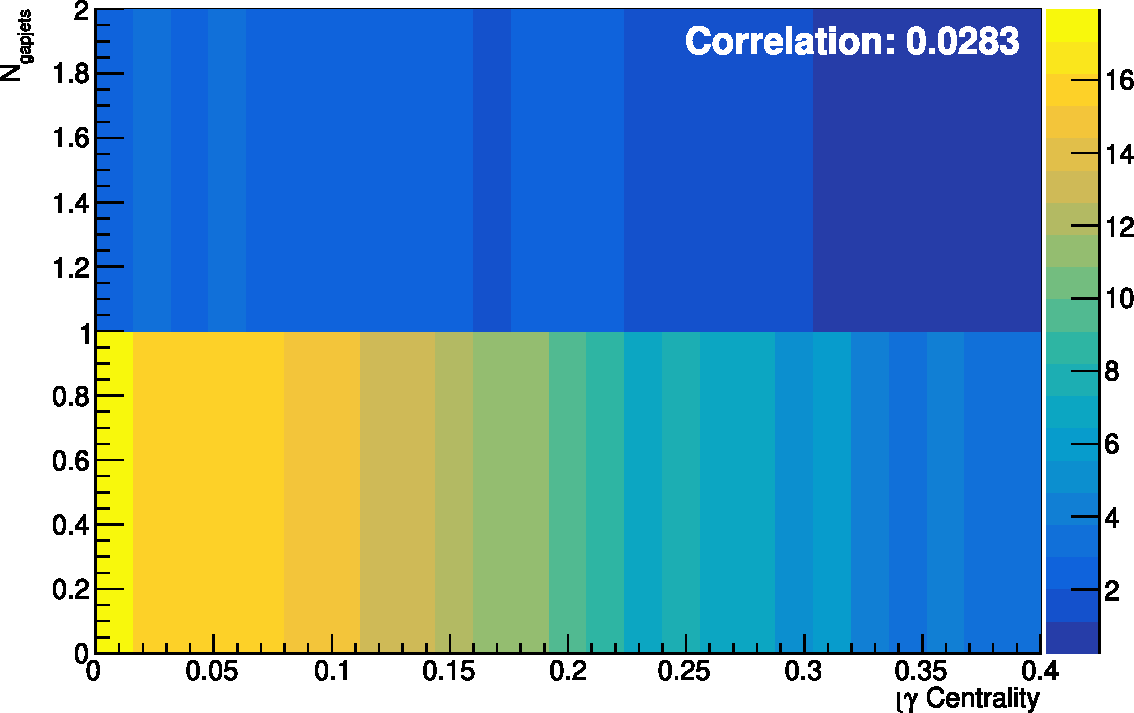
\includegraphics[width=\textwidth]{plots/diffx/correlations_ew.pdf}
    \caption{}
\end{subfigure}
\hfill
\begin{subfigure}[b]{0.48\textwidth}
    \centering
    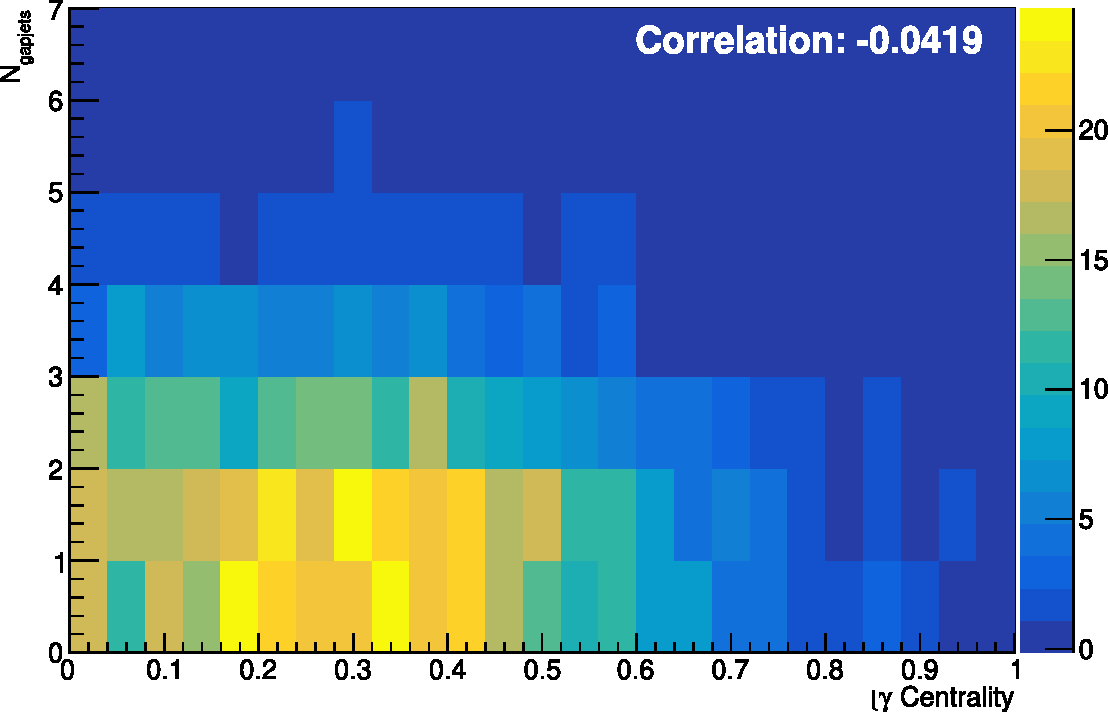
\includegraphics[width=\textwidth]{plots/diffx/correlations_qcd.pdf}
    \caption{}
\end{subfigure}
\caption{2D Histograms and correlation coefficients for \ewwy (a) and \qcdwy (b) of \xily centrality against \ngapjets. Note the scales are different for the two plots. Also note that the bins are not normalised. Because the cross-sections are larger at lower centrality and \ngapjets values, these bins have a higher occupancy. This does not imply a correlation between the two observables. The correlation coefficients are shown in the top right of the plots. \label{fig:vbswy:correlation}}
\end{figure}

\begin{table}[t]
  \centering
  \begin{tabular}{|l|c|c|}
  \hline
  Region & Selection & Abbreviation \\ \hline
  Signal Region & $\ngapjets = 0$, $\xily < 0.35$ & SR \\
  Control Region A & $\ngapjets = 0$, $0.35 \leq \xily < 1$ & CRa \\
  Control Region B & $\ngapjets \geq 1$, $0.35 \leq \xily < 1$ & CRb \\
  Control Region C & $\ngapjets \geq 1$, $\xily < 0.35$ & CRc \\
  \hline
  \end{tabular}
  \caption{\label{tab:vbswy:regions} The definitions of the signal and control regions used in the extraction of the \ewwy signal. The Signal Region has the requirements that there must be little hadronic activity in the rapidity interval between the tagging jets and that the reconstructed $\ell\gamma$ system is produced centrally relative to the tagging jets. The control regions are defined through inverting one or both of these cuts.}
\end{table}  
%
%\begin{figure}[t]
%  \centering
%  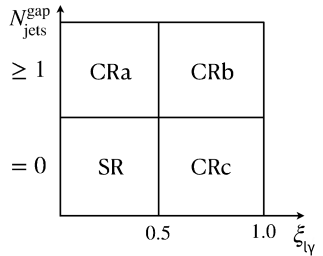
\includegraphics[width=0.50\textwidth]{plots/diffx/Control_regions.png}
%  \caption{Graphical representation of the signal and control regions used in the binned log-likelihood fit.\label{fig:vbswy:CRs}}
%\end{figure}
%
%\begin{figure}[t]
%\centering
%\begin{subfigure}[b]{0.48\textwidth}
%    \centering
%    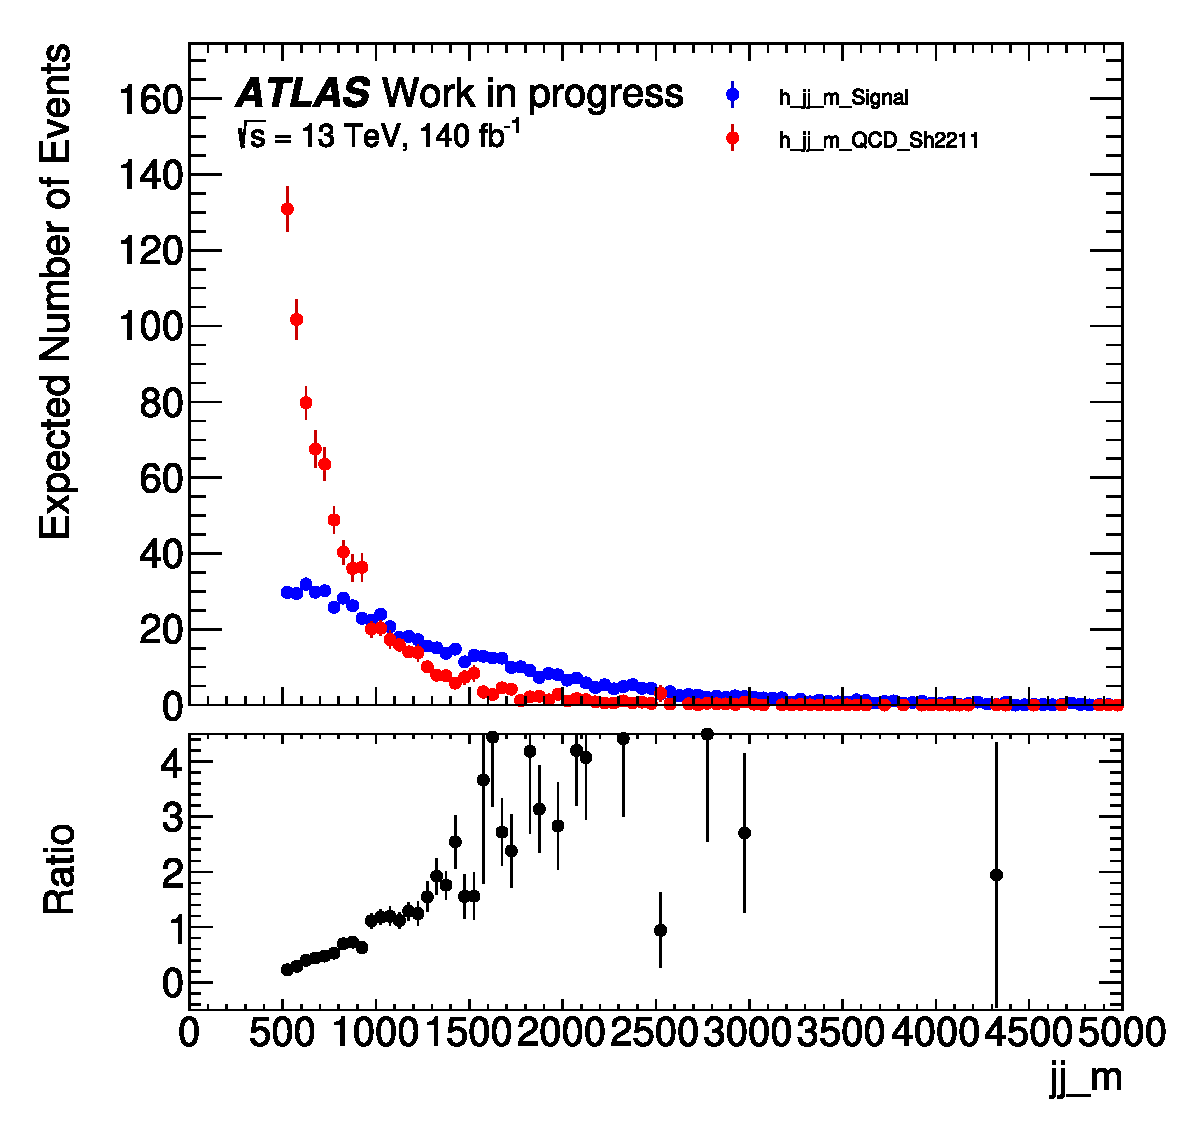
\includegraphics[width=\textwidth]{plots/diffx/comparison_signal_mg.pdf}
%    \caption{}
%\end{subfigure}
%\hfill
%\begin{subfigure}[b]{0.48\textwidth}
%    \centering
%    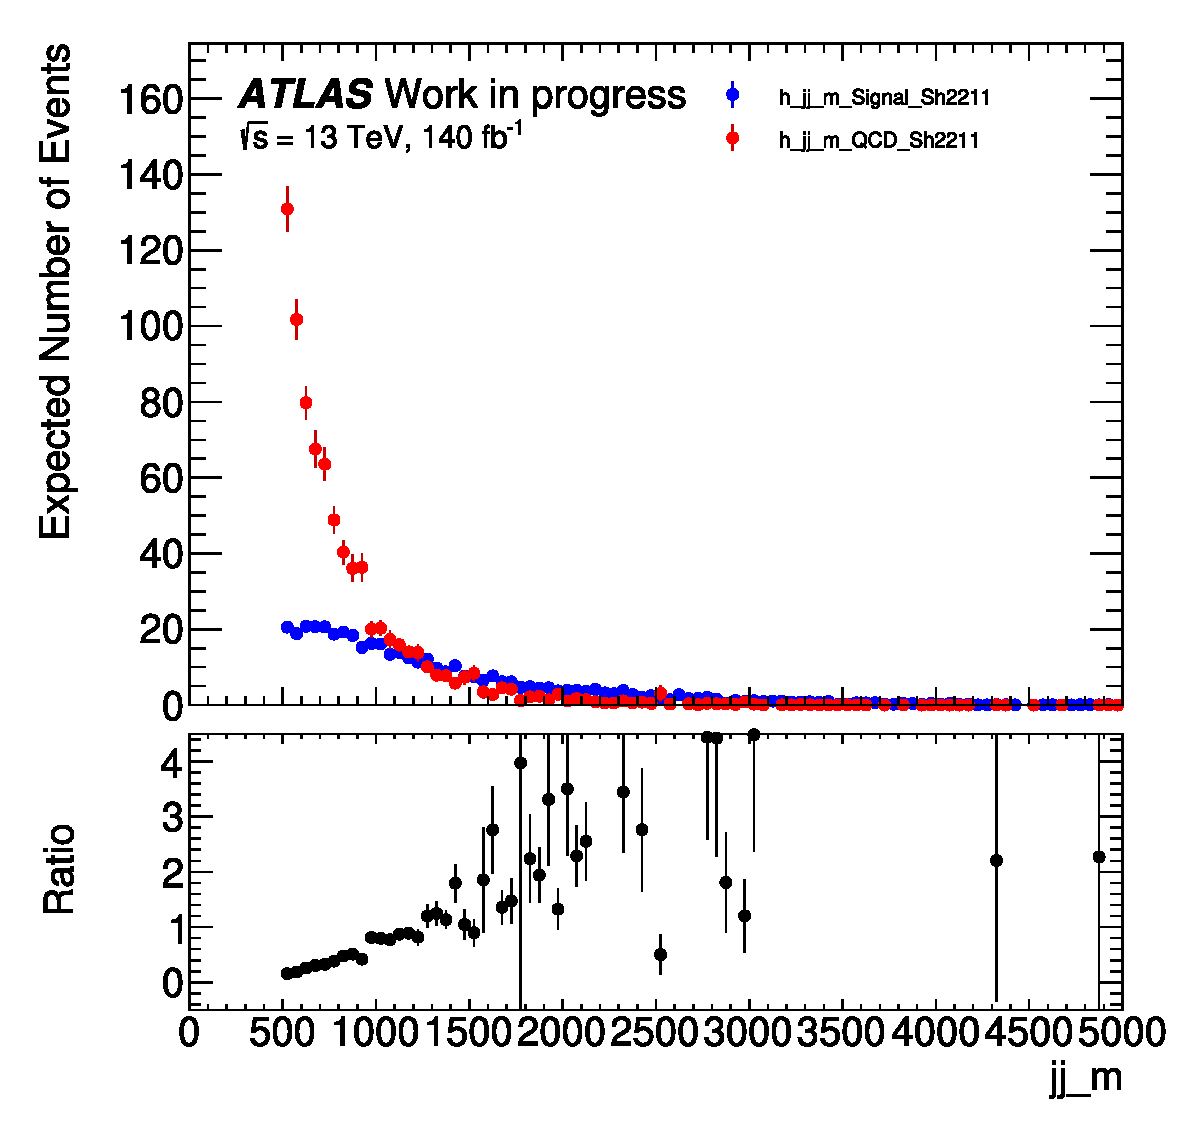
\includegraphics[width=\textwidth]{plots/diffx/comparison_signal_sh.pdf}
%    \caption{}
%\end{subfigure}
%\caption{The \qcdwy and \ewwy \mjj distributions for $\xily>0.35$. The left plot (a) shows the \MADGRAPH5 signal distribution in blue and the \SHERPA-2.2.11 QCD distribution in red. The right plot (b) shows the \SHERPA-2.2.11 signal distribution in blue and the \SHERPA-2.2.11 QCD distribution in red. The distributions overlap at around 1$\TeV$ for both plots, and the trade-off between number of signal events and the purity of those events is evident. Below around $1\TeV$, the \qcdwy event yield is $>50\%$ of the total $W\gamma jj$ yield, yielding larger uncertainties in the EW yield extracted using the likelihood fit method.\label{fig:signalandqcdmjj}}

%\end{figure}
This fit is used to constrain the shape and normalization of the \qcdwy background in addition to constraining the shape and normalisation of the \ewwy event yield. The fit is performed in the combined electron and muon channels, since it was not possible to derive separate lepton channel distributions due to statistical limitations. The signal region was blinded during the stage where analysis decisions and optimisations were being made.

The likelihood function is defined as (with indices $r,i$ running over regions and bins respectively)

\begin{equation}\label{eq:likelihood}
    L = \prod_{r,i} \text{Pois}(N^{\text{data}}_{ri} | \gamma_{ri}\nu_{ri}(\boldsymbol{\alpha})) \text{Pois}\left(\left(\frac{\nu_{ri}(\mathbf{1})}{\delta_{ri}}\right)^2 \Big{|} \gamma_{ri}\left(\frac{\nu_{ri}(\mathbf{1})}{\delta_{ri}}\right)^2\right),
\end{equation}

where $\nu_{ri}$ is the total MC estimate given by

\begin{equation}\label{eq:nu}
  \nu_{ri}=\mu_i\nu_{ri}^{\text{EW,MC}}+\nu_{ri}^{\text{strong}}+\nu_{ri}^{\text{other}},
\end{equation}

and the $\nu_{ri}^{\text{EW,MC}}$ is the MC prediction for the \ewwy event yield. $\nu_{ri}^{\text{other}}$ is the prediction for the non-\qcdwy background processes (Z$\gamma$jj, top, and non-prompt). $\mu_i$ is a free parameter in the fit, and represents the EW signal strength. The term $\nu_{ri}^{\text{strong}}$ is the prediction for the \qcdwy event yield, and is defined by

\begin{align}\label{eq:strongmcfit}
   \centering
   \nu_{\text{CRa},i}^{\text{strong}}=b_{\text{L},i}\nu_{\text{CRa},i}^{\text{strong,MC}}&,\hspace{5pt}
   \nu_{\text{CRb},i}^{\text{strong}}=b_{\text{H},i}\nu_{\text{CRb},i}^{\text{strong,MC}},\\
   \nu_{\text{SR},i}^{\text{strong}}=b_{\text{L},i}c\nu_{\text{SR},i}^{\text{strong,MC}}&,\hspace{5pt}
   \nu_{\text{CRc},i}^{\text{strong}}=b_{\text{H},i}c\nu_{\text{CRc},i}^{\text{strong,MC}},
   \label{eq:strongmcfit2}
\end{align}
where $\nu_{ri}^{\text{EW,MC}}$ are the MC predictions for the \qcdwy backgrounds. The parameters $b_{L,i}, b_{H,i}$ are responsible for constraining the \qcdwy background in regions of low and high centrality, respectively. The $c$ parameter is a constant and acts as a residual correction which accounts for non-closure when transferring the $b$ factors to the signal region.

The term $\text{Pois}(N|\lambda)$ in Equation \ref{eq:likelihood} is the Poisson probability mass function for $N$ events given the parameter $\lambda$. The vector $\boldsymbol{\alpha}$ contains all free parameters except $\gamma_{ri}$, i.e. 
\begin{equation}
  \boldsymbol{\alpha}\equiv(\mu_1,\ldots,\mu_n,b_{L,1},\ldots,b_{L,n},b_{H,1},\ldots,b_{H,n}, c).
\end{equation}
The number of bins is given by $n$, and $\gamma_{ri}$ is a nuisance parameter which accounts for the finite MC statistical precision. The inclusion of the Poisson constraint parameters $\gamma_{ri}$ gives the MC templates additional freedom to float within their statistical uncertainties. The $\gamma_{ri}$ are themselves constrained by the terms $\text{Pois}((\frac{\nu_{ri}}{\delta_{ri}})^2|\gamma_{ri}(\frac{\nu_{ri}}{\delta_{ri}})^2)$, where the $\delta_{ri}$ denote the statistical uncertainty on the MC estimate. These constraint terms come about by treating the MC estimate as an auxiliary measurement with the relative stat uncertainty given by $\frac{\nu_{ri}(\mathbf{1})}{\delta_{ri}}$ \cite{VBSWy:likelihood}. The ``Beeston-Barlow'' \cite{VBSWy:beestonbarlow} treatment to MC stat uncertainties is used where the Poisson constraint parameter $\gamma_{ri}$ is shared between the MC samples that enter the likelihood. This has the implication that $\nu_{ri}(\mathbf{1})$ is implicitly a sum over all MC samples and the MC error $\delta_{ri}$ is the quadrature sum of all the MC statistical errors of all the samples.

Note that there is no Gaussian constraint term for systematic uncertainty nuisance parameters in the likelihood. This is because each systematic variation of MC simulations is fit separately and the difference in event yield between the nominal and systematic variation post-fit is taken to be the systematic uncertainty (before smoothing) in the extracted yield. This is covered in more detail in section \ref{sec:vbswy:extraction_uncertainties} and is equivalent to the approach where all systematic uncertainties are simultaneously constrained through the inclusion of Gaussian constrained nuisance parameters in the likelihood. The reason for using the former approach is because makes it simpler to propagate each systematic variation through the unfolding procedure.

\subsection{Choice of Model Parameters}\label{sec:ngapjets_crosscheck}

The choice for the set of floating parameters in the likelihood as described in \cref{eq:nu,eq:strongmcfit,eq:strongmcfit2} is motivated as follows. The simplest possible configuration would be to constrain the background using one control region where either the \ngapjets or \xily cut is inverted. The problem with inverting the centrality cut is that there are very few events in CRc, at high centrality. This could be overcome by lowering the centrality threshold, but then the purity of the \ewwy signal becomes significantly worse, resulting in larger modelling uncertainties. Inverting the \Ngapjets cut gives a control region with a greater event yield, however, this results in a large non-closure as the jet multiplicity distribution is not well modelled. In this one control region configuration, there are as many floating parameters as there are degrees of freedom, hence it is not possible to introduce another floating parameter to account for the modelling differences across the \ngapjets boundary. 

In the nominal three control region method described by \Cref{eq:likelihood,eq:nu,eq:strongmcfit}, two signal-like regions are defined, namely SR and CRc, alongside their corresponding control regions CRa, and CRb. The two constraint factors \bl and \bh are applied to the \qcdwy background in SR and CRc respectively, where L and H denote ``Low'' and ``High'' centrality. These factors are primarily constrained in CRa and CRb, respectively. This is because CRa and CRb have high event yields and higher background purity. Hence, changes to the signal strength will have little to no effect on the post-fit event yields, and conversely, changes to the \bi factors will have a large effect. 

With fewer free parameters than the available DoF, one has the freedom to define an additional floating parameter $c$, which is shared between the signal-like regions SR and CRc. This parameter acts to correct any non-closure in applying deriving \bl and \bh at large \ngapjets and then applying them at low \ngapjets. The number of parameters in the fit is given by $3\nbins+1$. The residual correction $c$ is chosen to be a constant rather than a polynomial. This choice is discussed in further detail in Section \ref{sec:vbswy:fitinstab}.
This method to constrain the dominant background was first developed for the ATLAS EW $Z$jj measurement \cite{VBSWy:VBFZ}. 

The default method is to use CRa to derive the of bin-dependent factors $b_i$ with the signal region (this is called the \textit{CRa method}). This is not the only reasonable choice. CRc could be chosen to derive the $b_i$ parameters (the \textit{CRc method}). These two configurations are equivalent, ignoring statistical effects \cite{VBSWy:VBFZ}. Ultimately, the CRa method is chosen as the nominal method because CRa has larger event yields compared to CRc. The effects of smaller statistics in CRc will be discussed in Section \ref{sec:vbswy:crosschecks}. The CRc method serves as a cross-check.

\section{Shape Dependence of \Ngapjet and \xily}

A large shape difference between the observed data and the MC predictions of the \xily and \ngapjets distributions would not be desirable, as this would imply that the strong constraint derived in a control region would not do well to constrain the same background in the SR. Figure \ref{fig:centralityngapjets} shows the normalised number of events as a function of \ngapjets and \xily for data with all predictions subtracted except for the \qcdwy MC prediction. These are shown separately at high \ngapjets (CRa + CRb) and at high \lyxi (CRb + CRc). The reason for not showing the \ngapjets shape at low \lyxi and the \lyxi shape at low \ngapjets is that this would correspond to unblinding the data. Figures \ref{biasa} and \ref{biasc} show that the shape of the \ngapjets distribution in data agrees with the prediction from simulation within \qcdwy generator choice uncertainties. Figures \ref{biasb} and \ref{biasd} show that the shape of the \xily distribution is consistent with simulation, after accounting for \qcdwy and \ewwy generator choice uncertainties and statistical uncertainties in the data and simulation.

\begin{figure}[t]
  \begin{subfigure}[b]{0.48\textwidth}
    \centering
    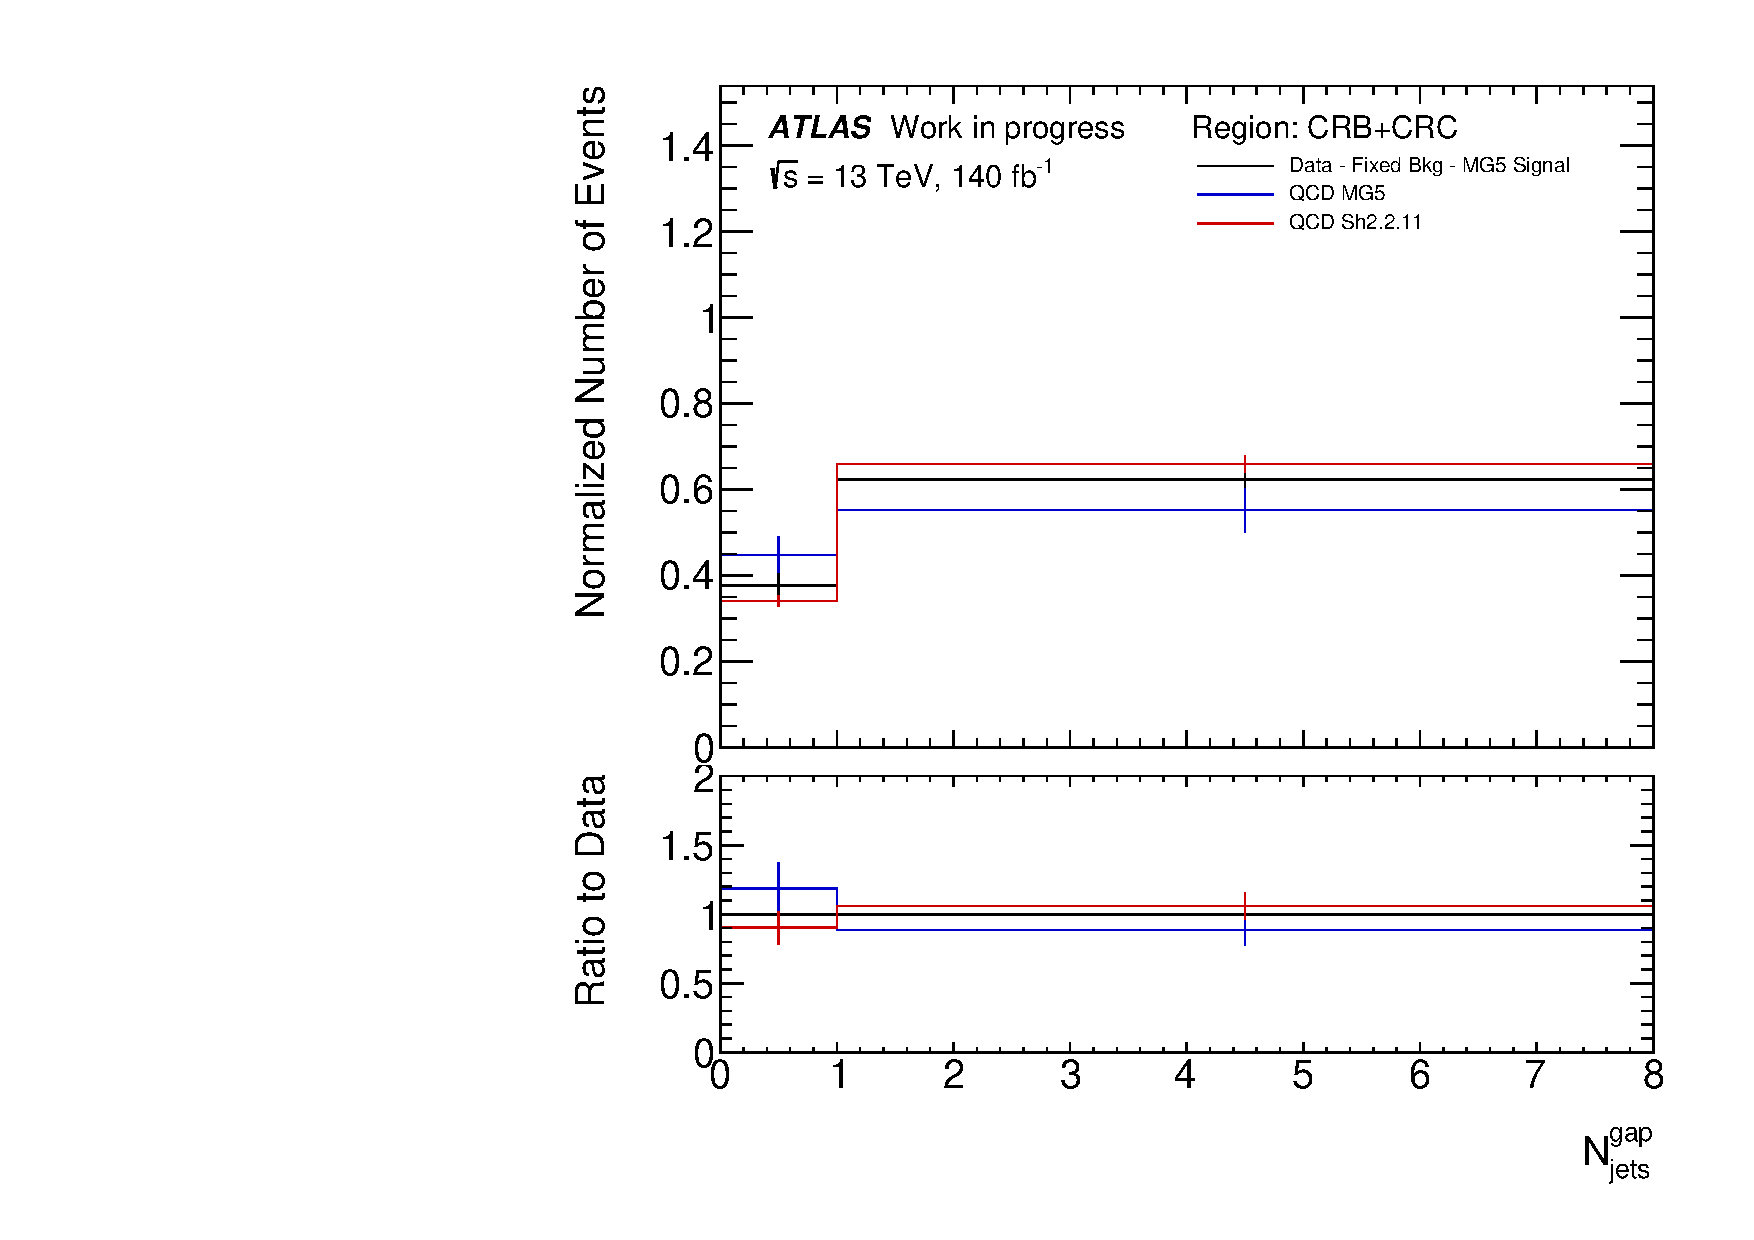
\includegraphics[width=\textwidth]{plots/diffx/biastest_13Feb_mgsignal_twobins_N_gapjets.pdf}
    \caption{\label{biasa}}
  \end{subfigure}
  \hfill
  \begin{subfigure}[b]{0.48\textwidth}
    \centering
    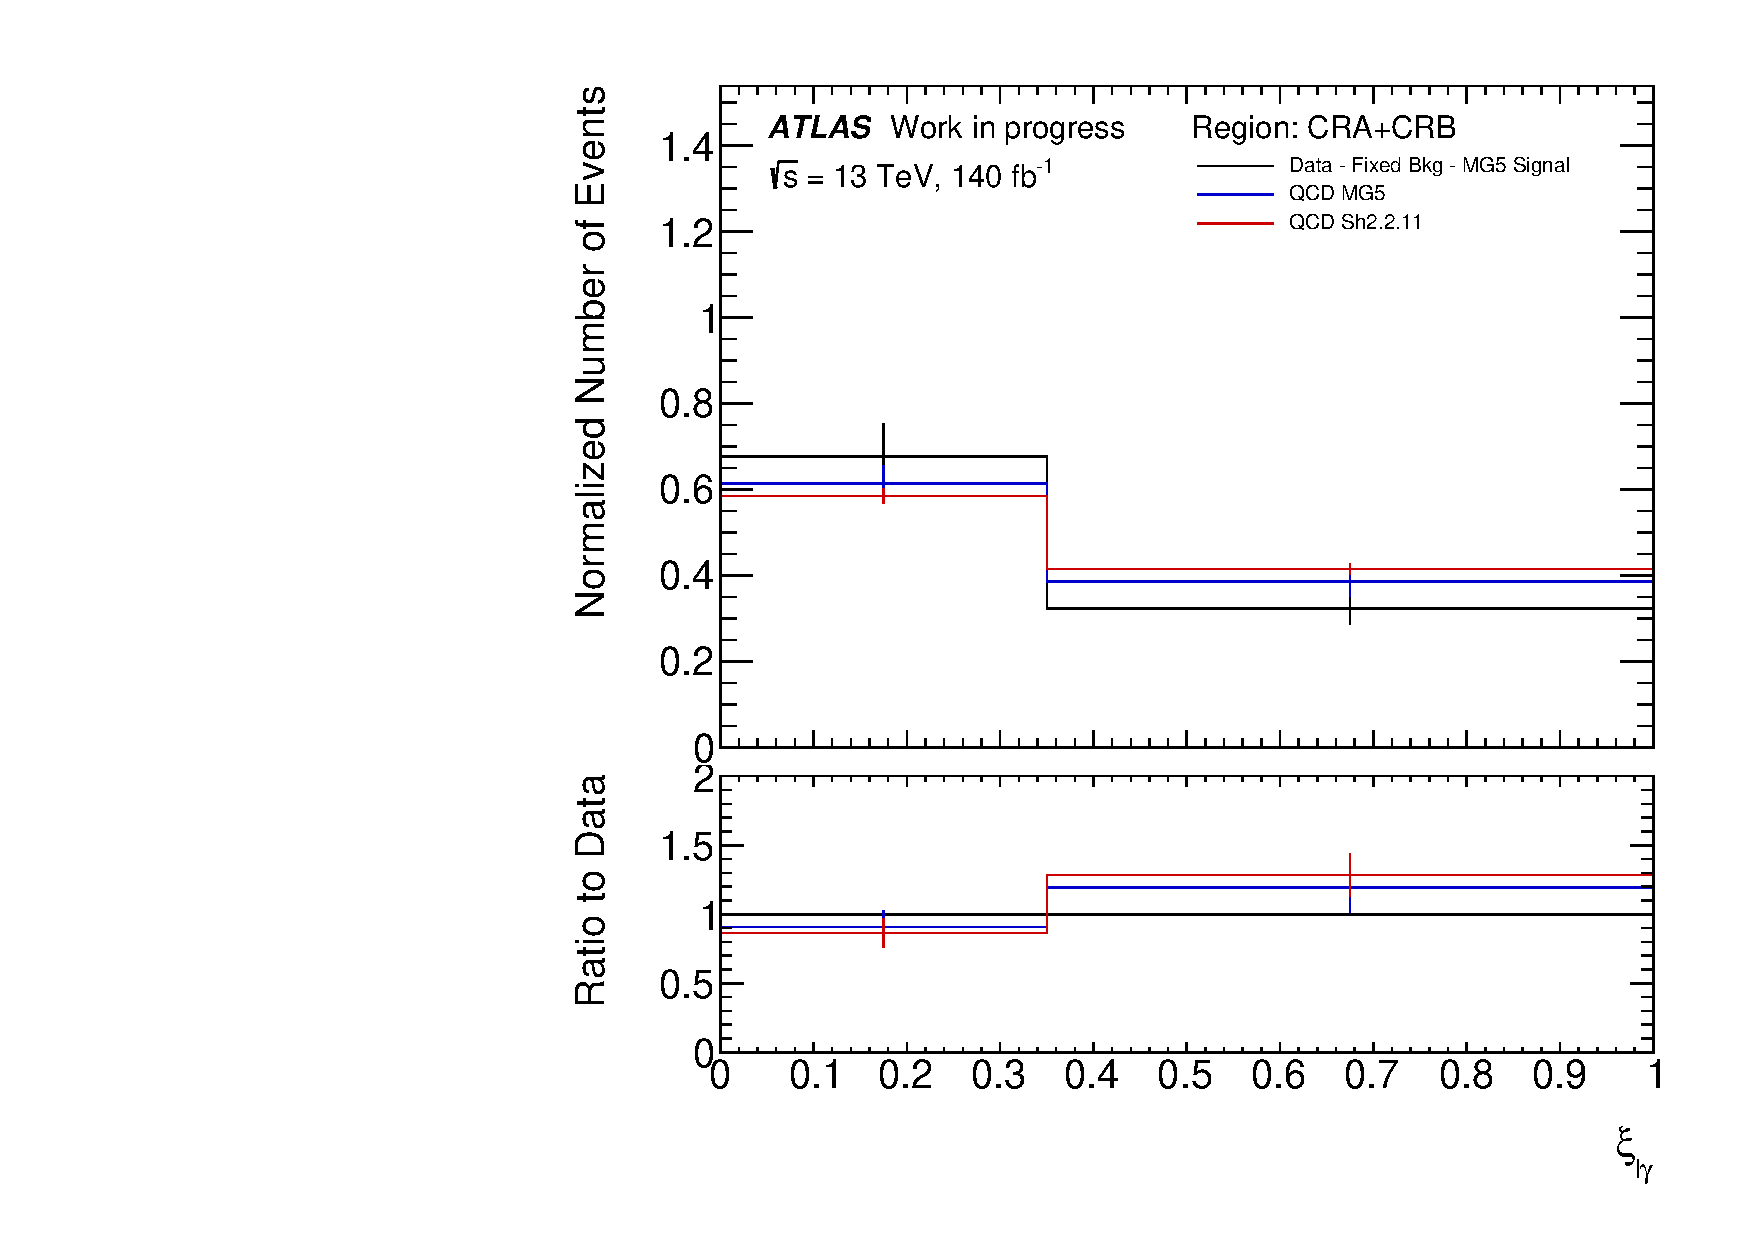
\includegraphics[width=\textwidth]{plots/diffx/biastest_13Feb_mgsignal_twobins_ly_centrality.pdf}
    \caption{\label{biasb}}
  \end{subfigure}
  \hfill
  \begin{subfigure}[b]{0.48\textwidth}
    \centering
    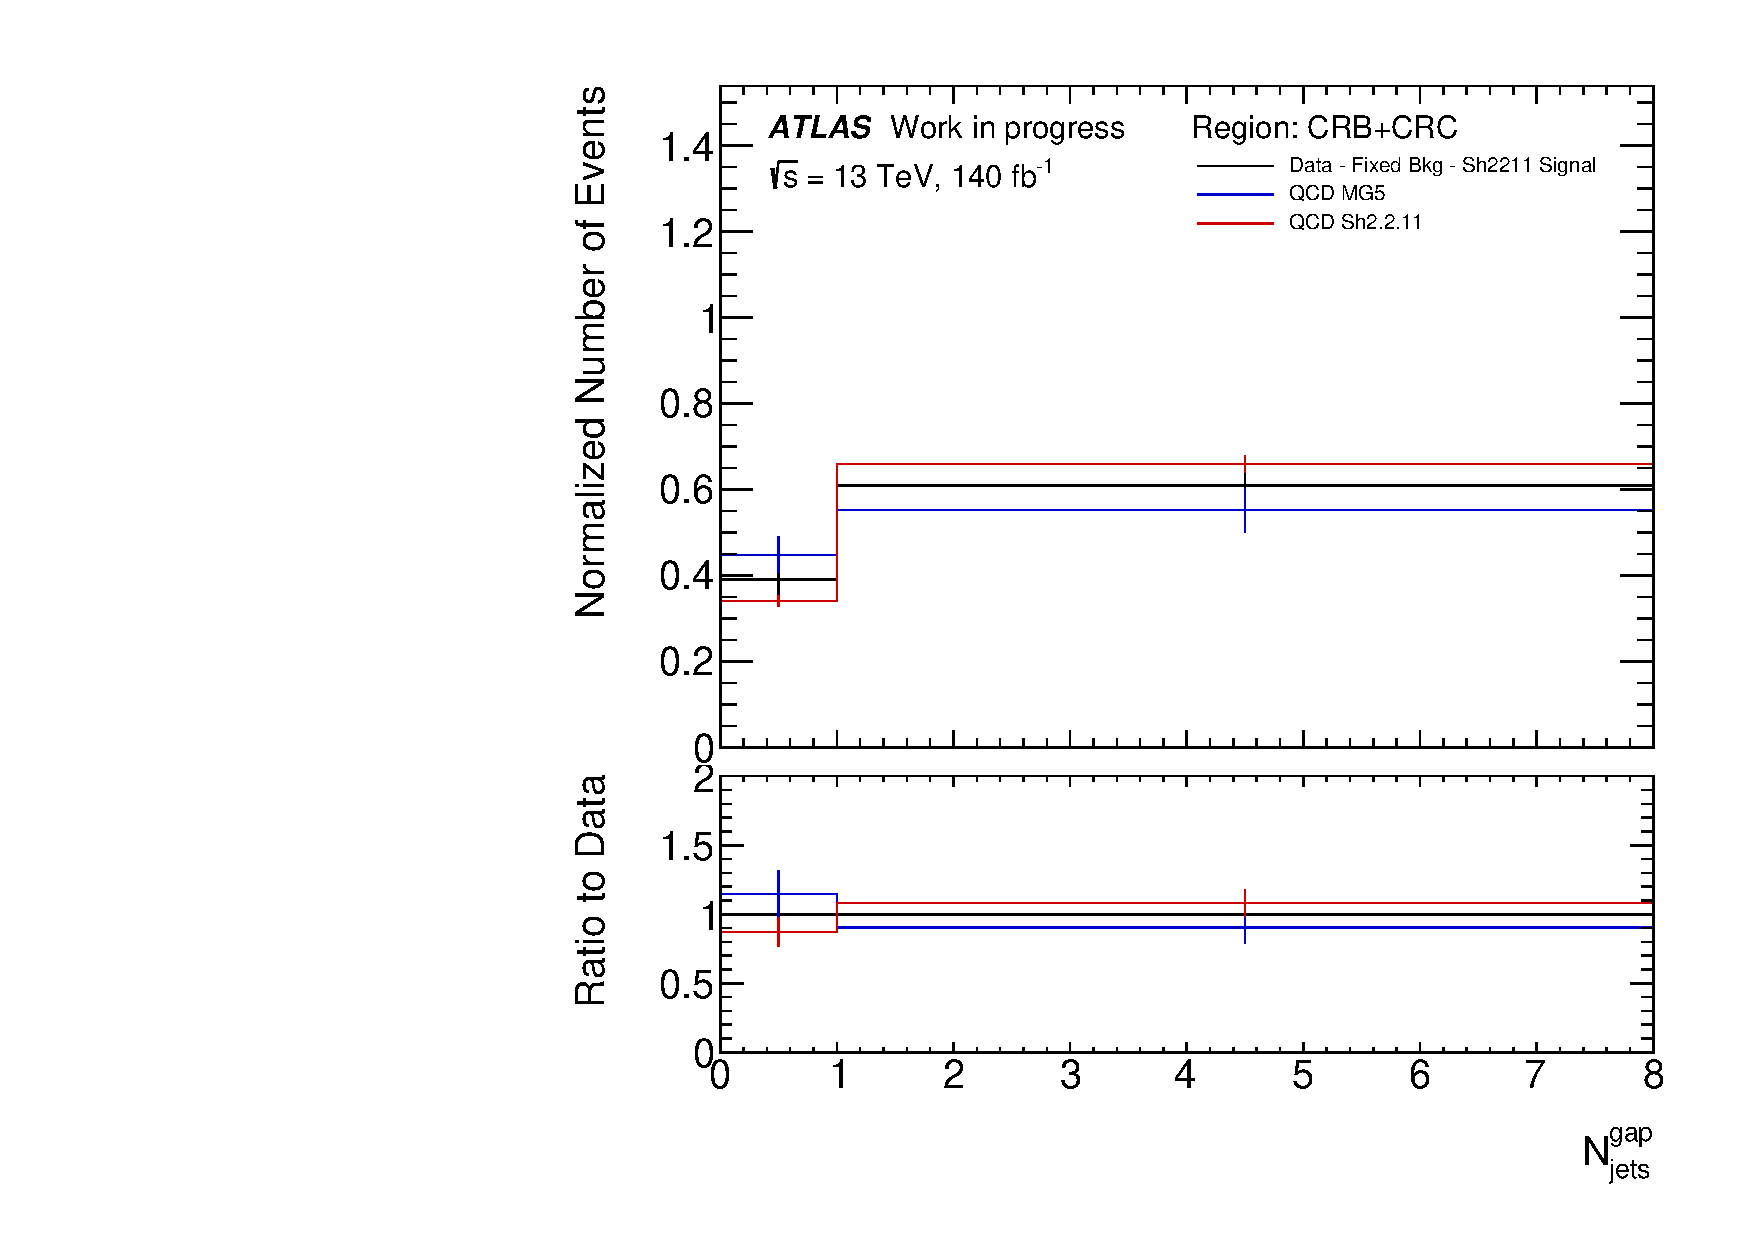
\includegraphics[width=\textwidth]{plots/diffx/biastest_13Feb_shsignal_twobins_N_gapjets.pdf}%\hspace{8pt}
    \caption{\label{biasc}}
  \end{subfigure}
  \hfill
  \begin{subfigure}[b]{0.48\textwidth}
    \centering
    %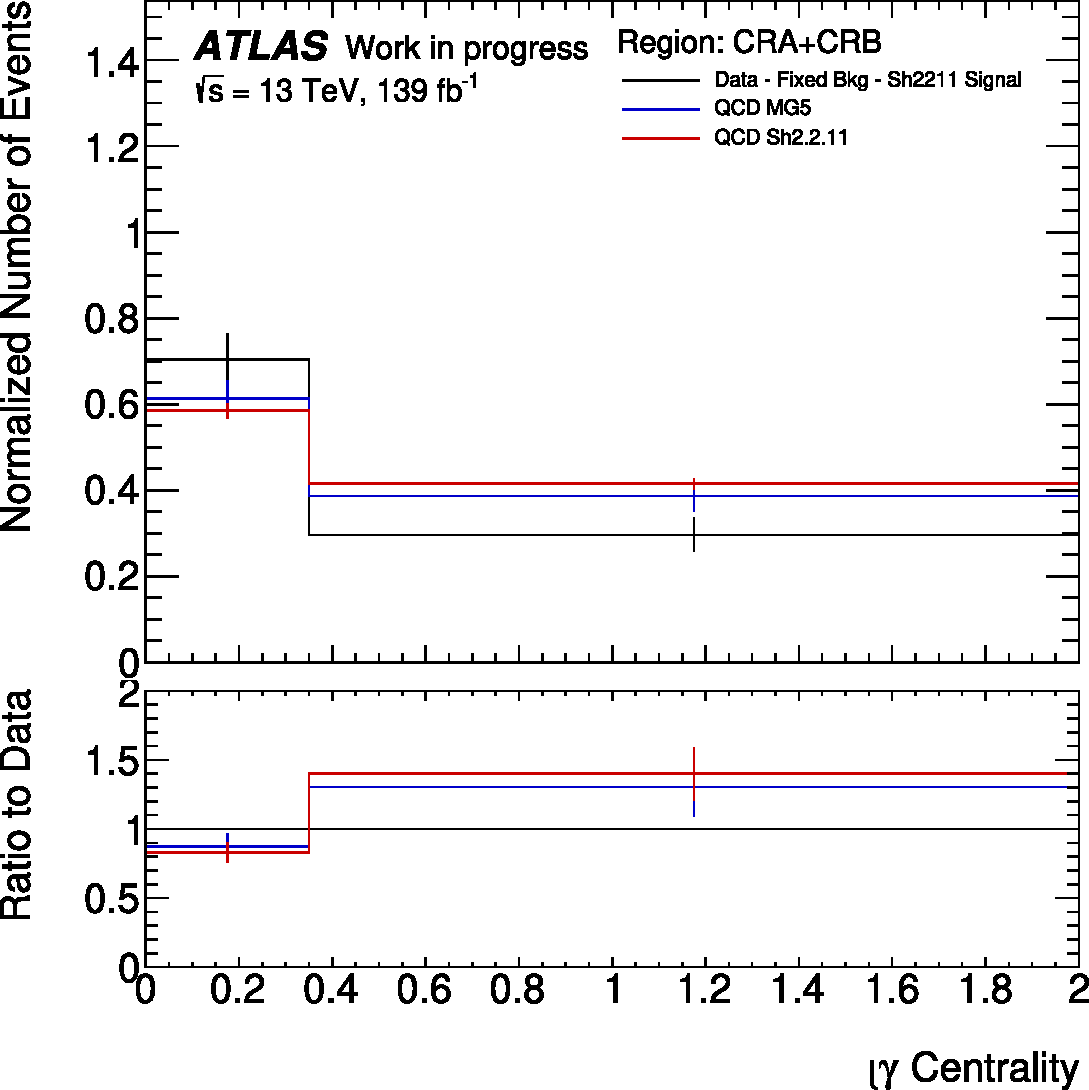
\includegraphics[width=0.45\textwidth]{plots/diffx/biastest_lycentrality_sherpa.pdf}
    %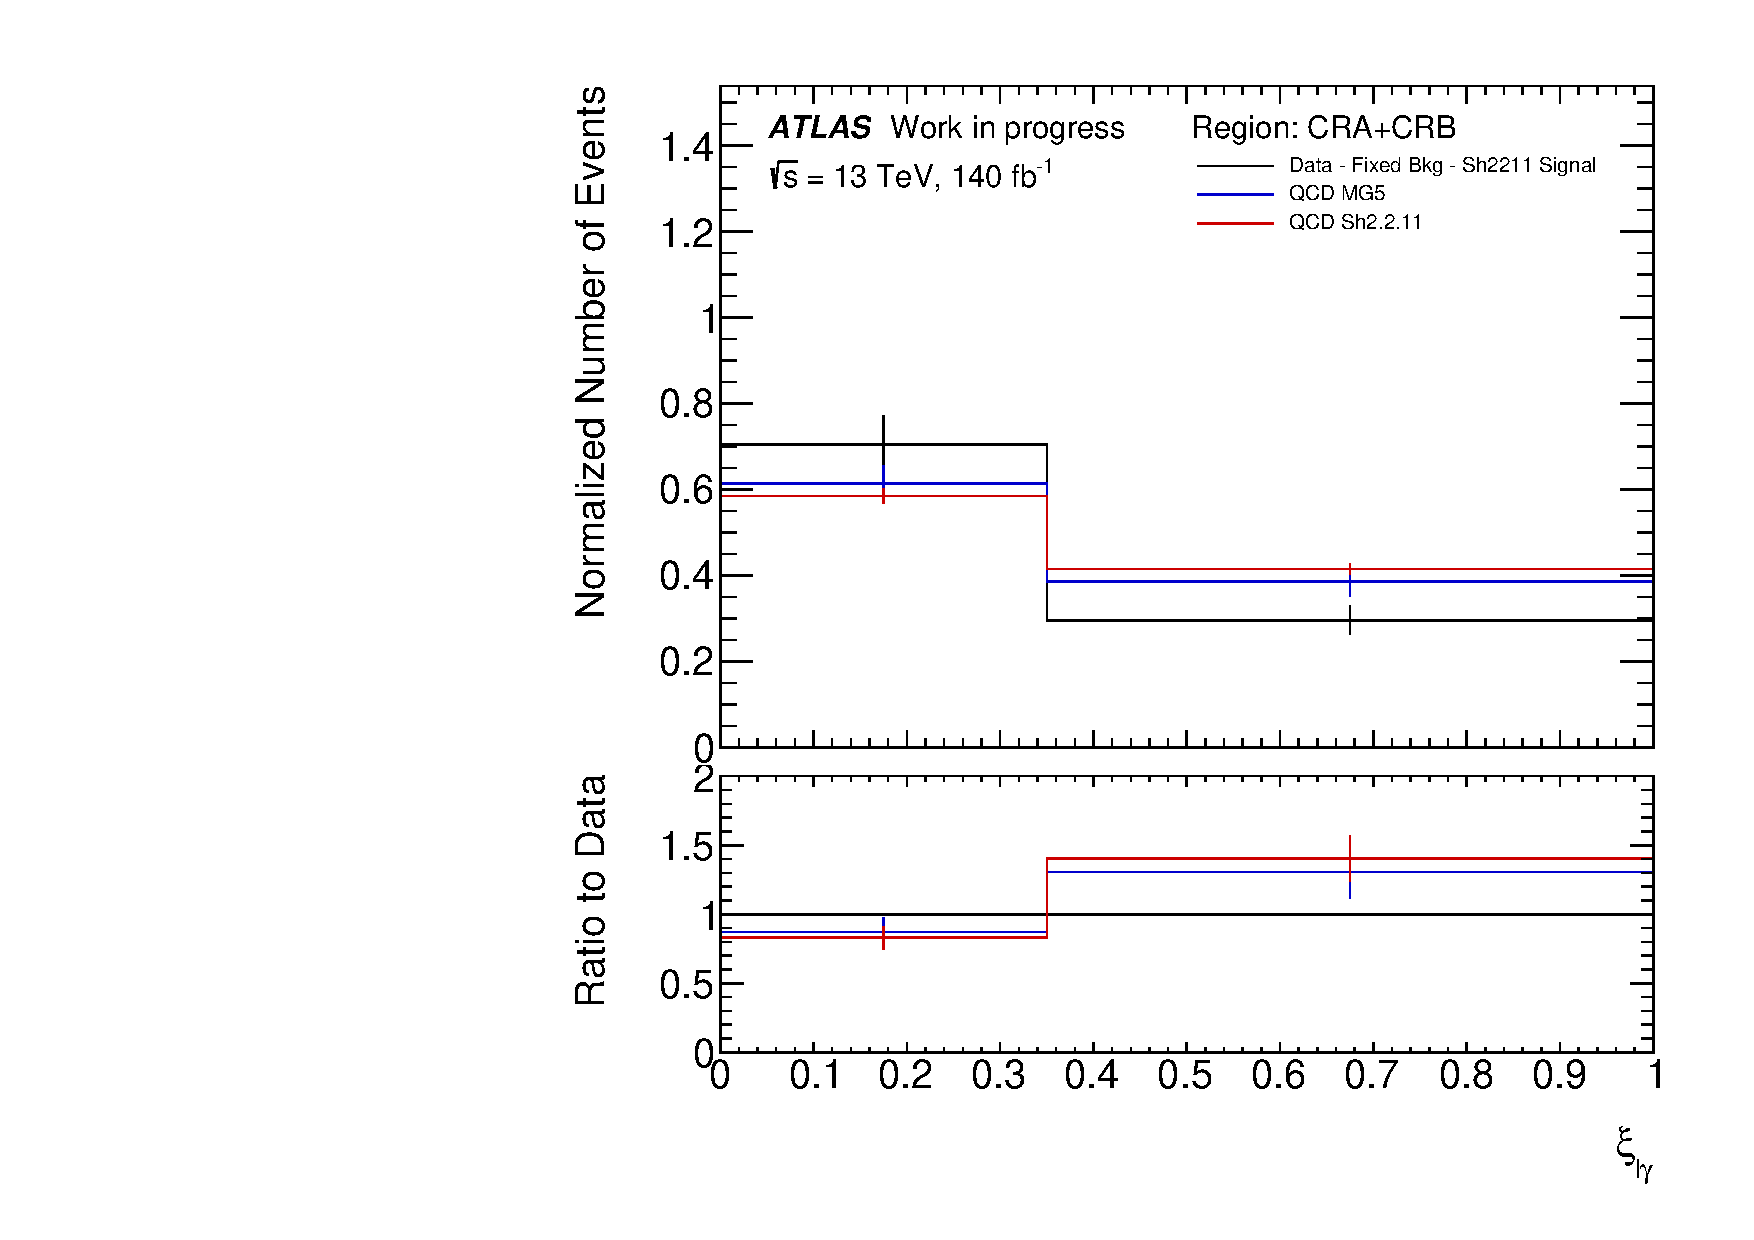
\includegraphics[width=0.94\textwidth]{plots/diffx/biastest_13Feb_shsignal_twobins_ly_centrality.pdf}
    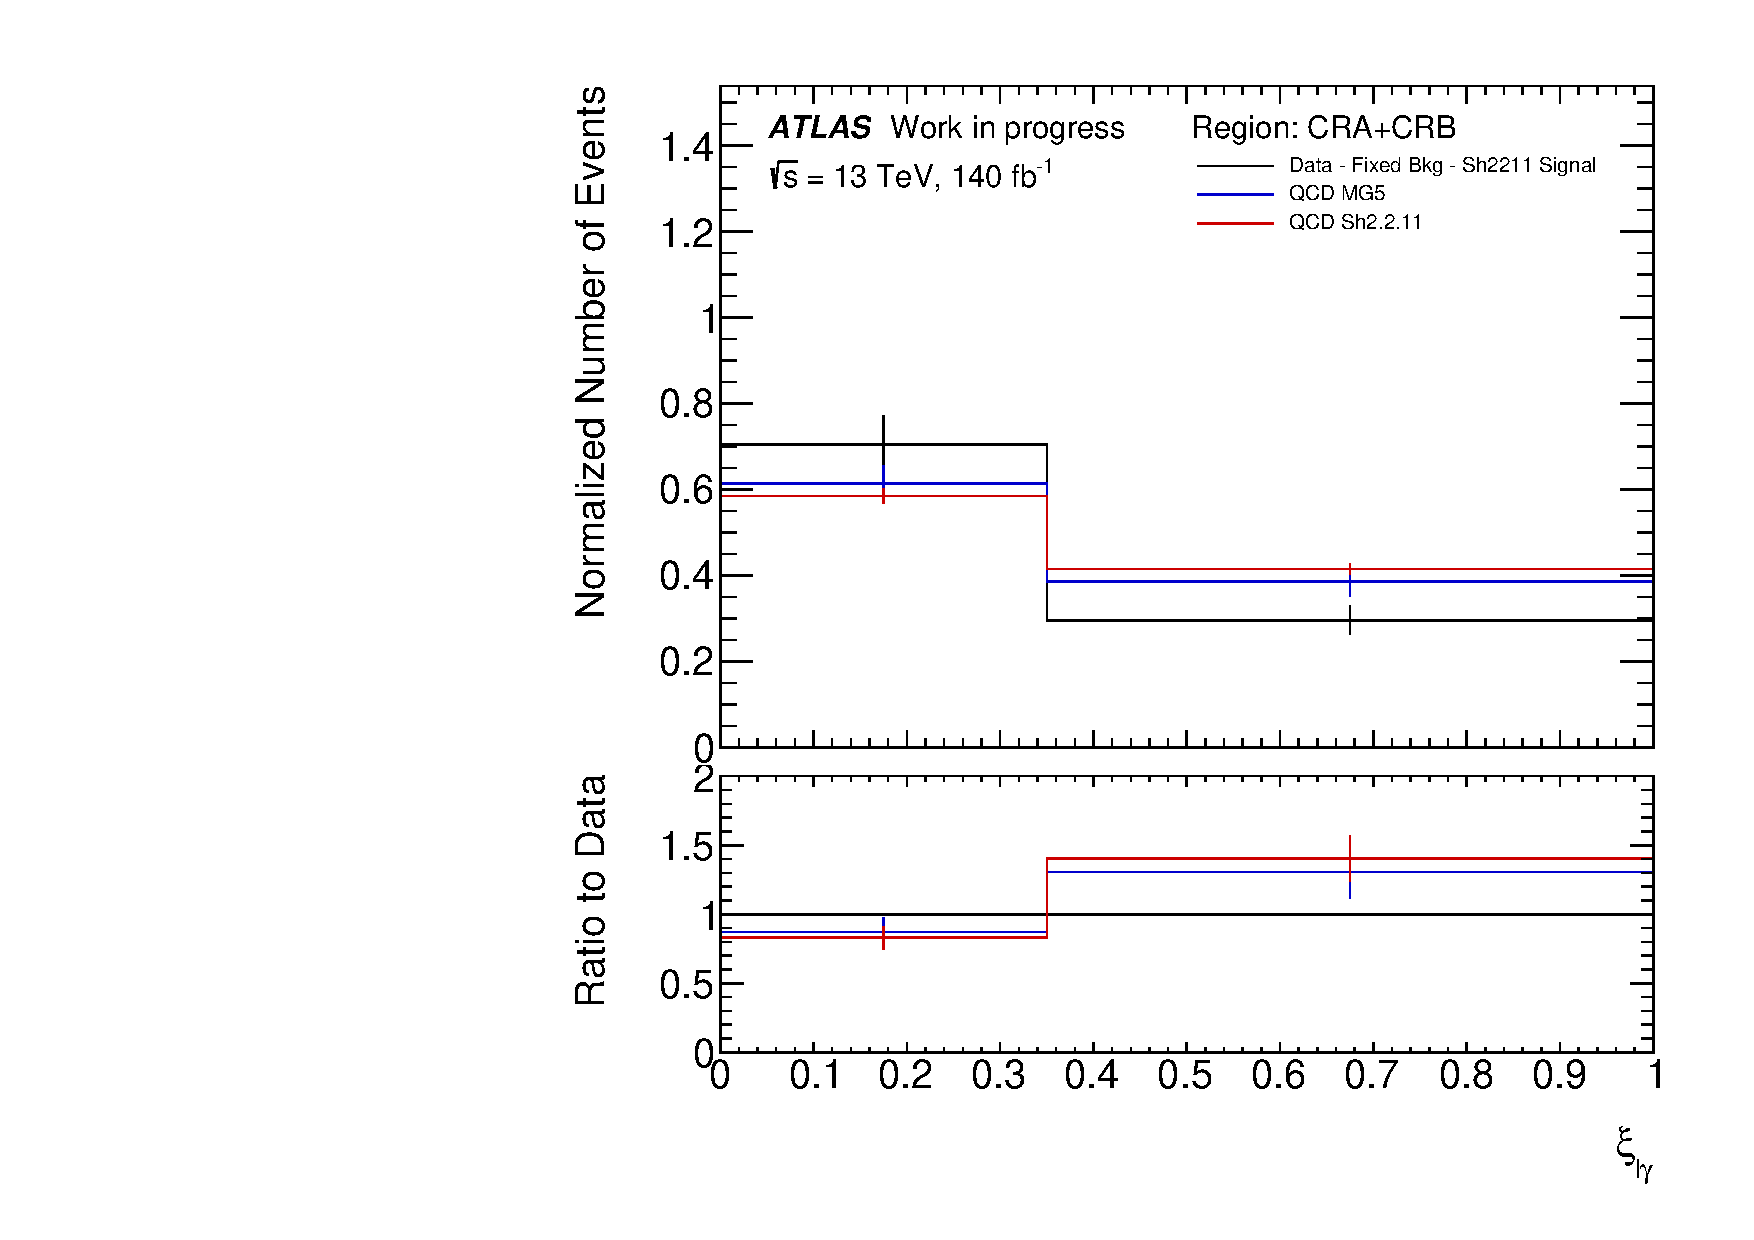
\includegraphics[width=\textwidth]{plots/diffx/biastest_13Feb_shsignal_twobins_ly_centrality.pdf}
    \caption{\label{biasd}}
  \end{subfigure}
  \caption{The \Ngapjets distribution is shown in (a,c), and the \xily in (b,d). The top two plots (a,b) show the results where the \SHERPA-2.2.11 \ewwy MC sample is used, and the bottom two plots (c,d) show the results where the \MADGRAPH5 \ewwy MC sample is used. The shape differences between data - [fixed background + signal] (black line) and the \qcdwy MC predictions (red and blue lines) are shown in the top canvas. The bottom canvas shows the ratio between the purely MC and data-MC predictions. The error bars on the black lines in the ratio plot are the data statistical uncertainty combined with the MC statistical uncertainty in the ratio. The error bars on the red and blue lines correspond to the MC statistical uncertainty.}
  \label{fig:centralityngapjets}
\end{figure}

\section{Construction of the Asimov Dataset}

To prevent any unintended bias, e.g. tuning of parameters so that the data match the simulation, the data were blinded in the signal region until the analysis was formally approved. The analysis was optimised using a dataset which acts as a proxy for real data, called an Asimov dataset. The number of events in the Asimov sample is given by $N^{\text{Asimov}}_{ri}=\sum_{s}\nu_{ri}^{s\text{,MC}}$, where the index $s$ runs over the \ewwy, \qcdwy, non-prompt, top, and $Z\gamma$jj samples. The indices $r$ and $i$ run over the regions, and the observable bins, respectively. The \qcdwy background used in the Asimov is the nominal \SHERPA 2.2.11 sample. However, for certain tests an alternative Asimov dataset is constructed using the \MADGRAPH \qcdwy sample. It is explicitly stated whenever this alternative Asimov dataset is used. The Asimov statistical uncertainties are given by $\sqrt{N^{\text{Asimov}}_{ri}}$.

\section{Binning Determination}\label{sec:vbswy:binning}

The binning is determined for each observable using the following criteria: 
\begin{itemize}
  \item The relative statistical precision of the extracted \ewwy yield must be similar across the bins.
  \item The bin width must be at least as large as twice the detector resolution in that bin.
\end{itemize}

For the angular observables, \dphisigned and \lepgamdphi, the range is designed by geometry to be $[-\pi,\pi]$. For the kinematic observables, the upper bound $k$ is chosen to be at a value in which there is at most one expected event in the interval $[k,\infty]$. 

Since the analysis optimisations were performed blinded, the binning was determined using the Asimov dataset. The binning was initially optimised to target statistical uncertainty in each bin of about 30-35\%, they were then adjusted to account ensure adequate detector resolution.

\subsection{Detector Resolution with Bin Width}

If the detector resolution is large relative to the bin width, the unfolding will have to correct for a larger amount of bin migrations. This step relies on the MC simulation of the signal. Therefore, by requiring the resolution to be small relative to the bin width, the model dependence of the measurement in reduced. 

The \ewwy predictions in the signal region are used to estimate the measurement variable resolution in each bin. The set of events which pass the reco-level selections in Table \ref{tab:vbswy:analysiscuts} are stored in a 2-dimensional histogram of truth-variable vs reco-variable. Within each reco bin, a fine truth bin splitting is chosen such that a Gaussian can be fit over the truth predictions. The width of this Gaussian is taken to be the resolution. Comparisons of these resolution values to the width of the bins are shown in Figure \ref{fig:vbswy:resolutionsrebin}. A bin is sufficiently wide if the bin width is at least twice the averaged resolution.

\begin{figure}[t]
\centering
\begin{subfigure}[b]{0.48\textwidth}
    \centering
    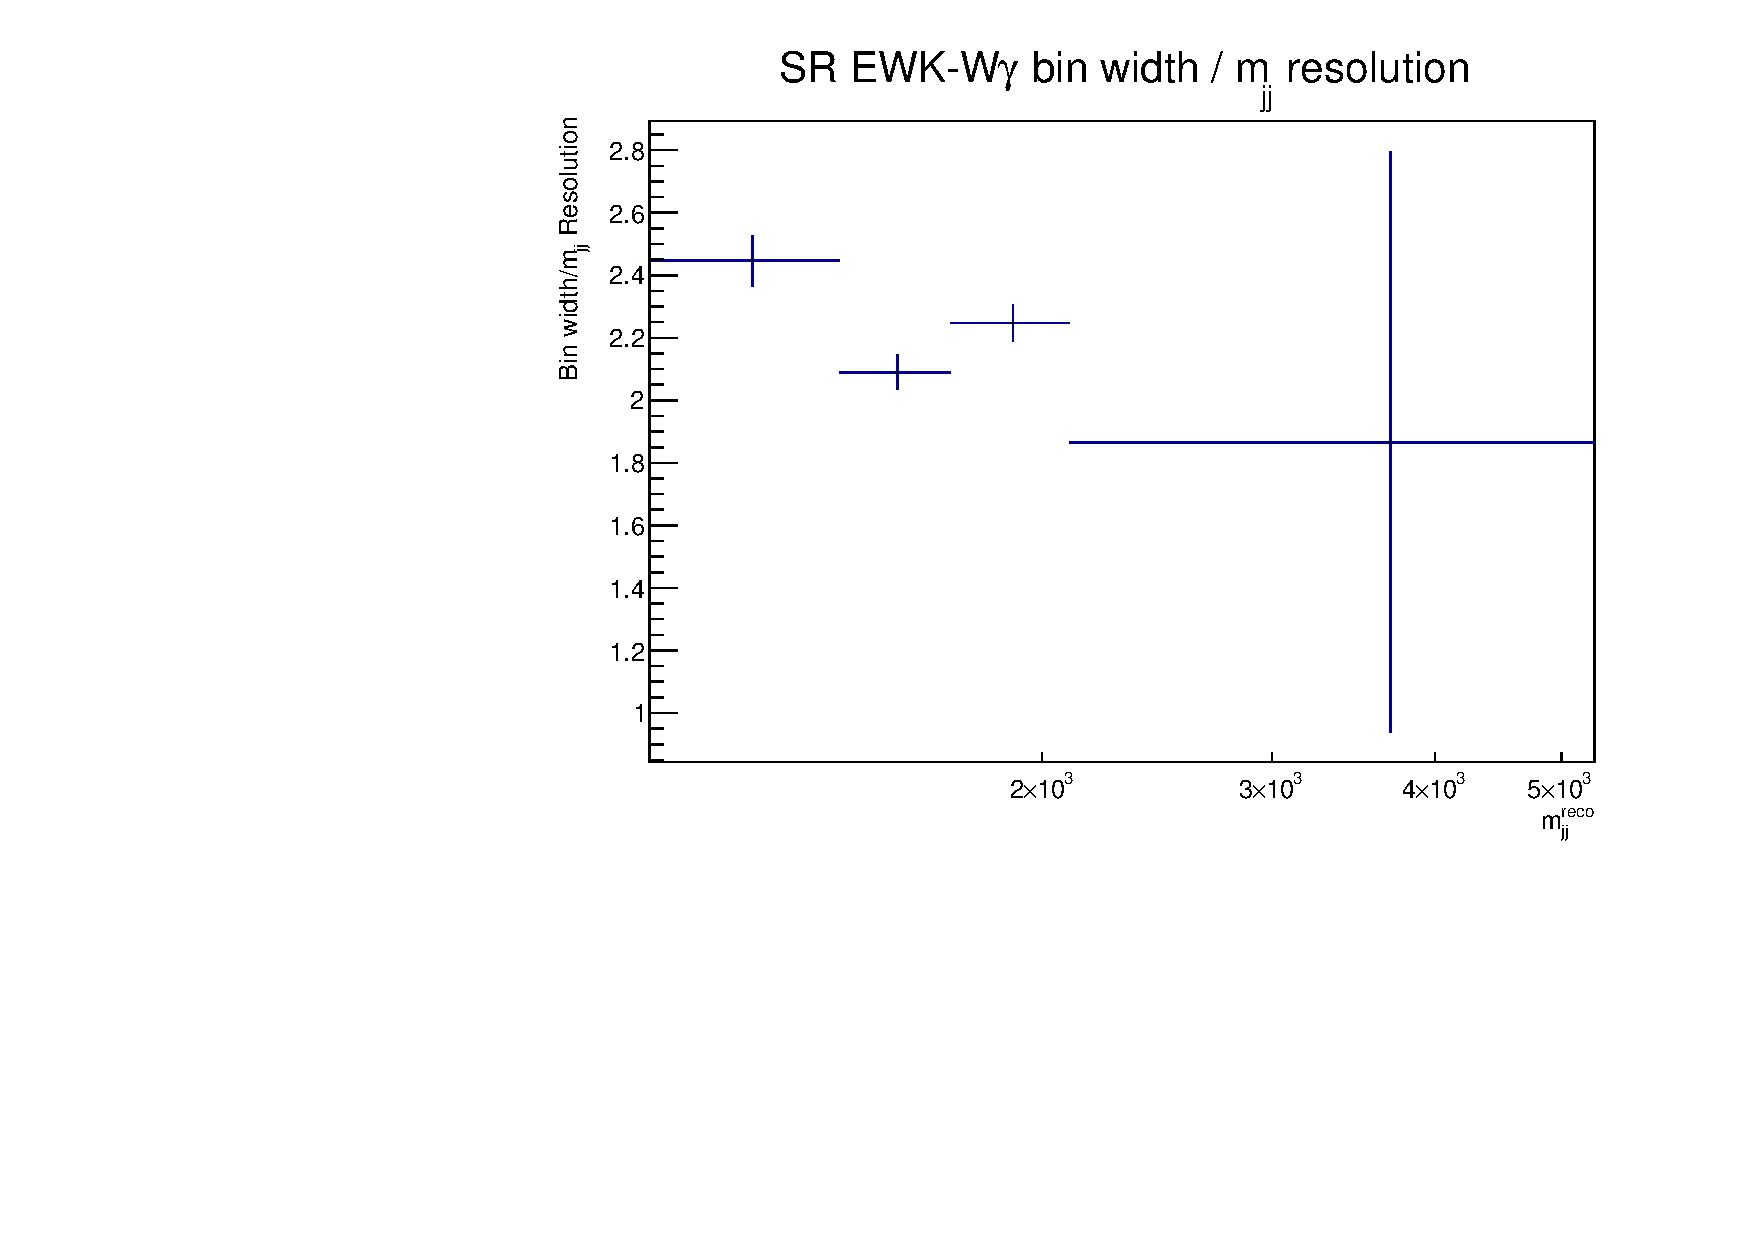
\includegraphics[width=\textwidth]{plots/diffx/binning/jj_m_resolutions_rebin_SR.pdf}
    \caption{}
\end{subfigure}
\hfill
\begin{subfigure}[b]{0.48\textwidth}
    \centering
    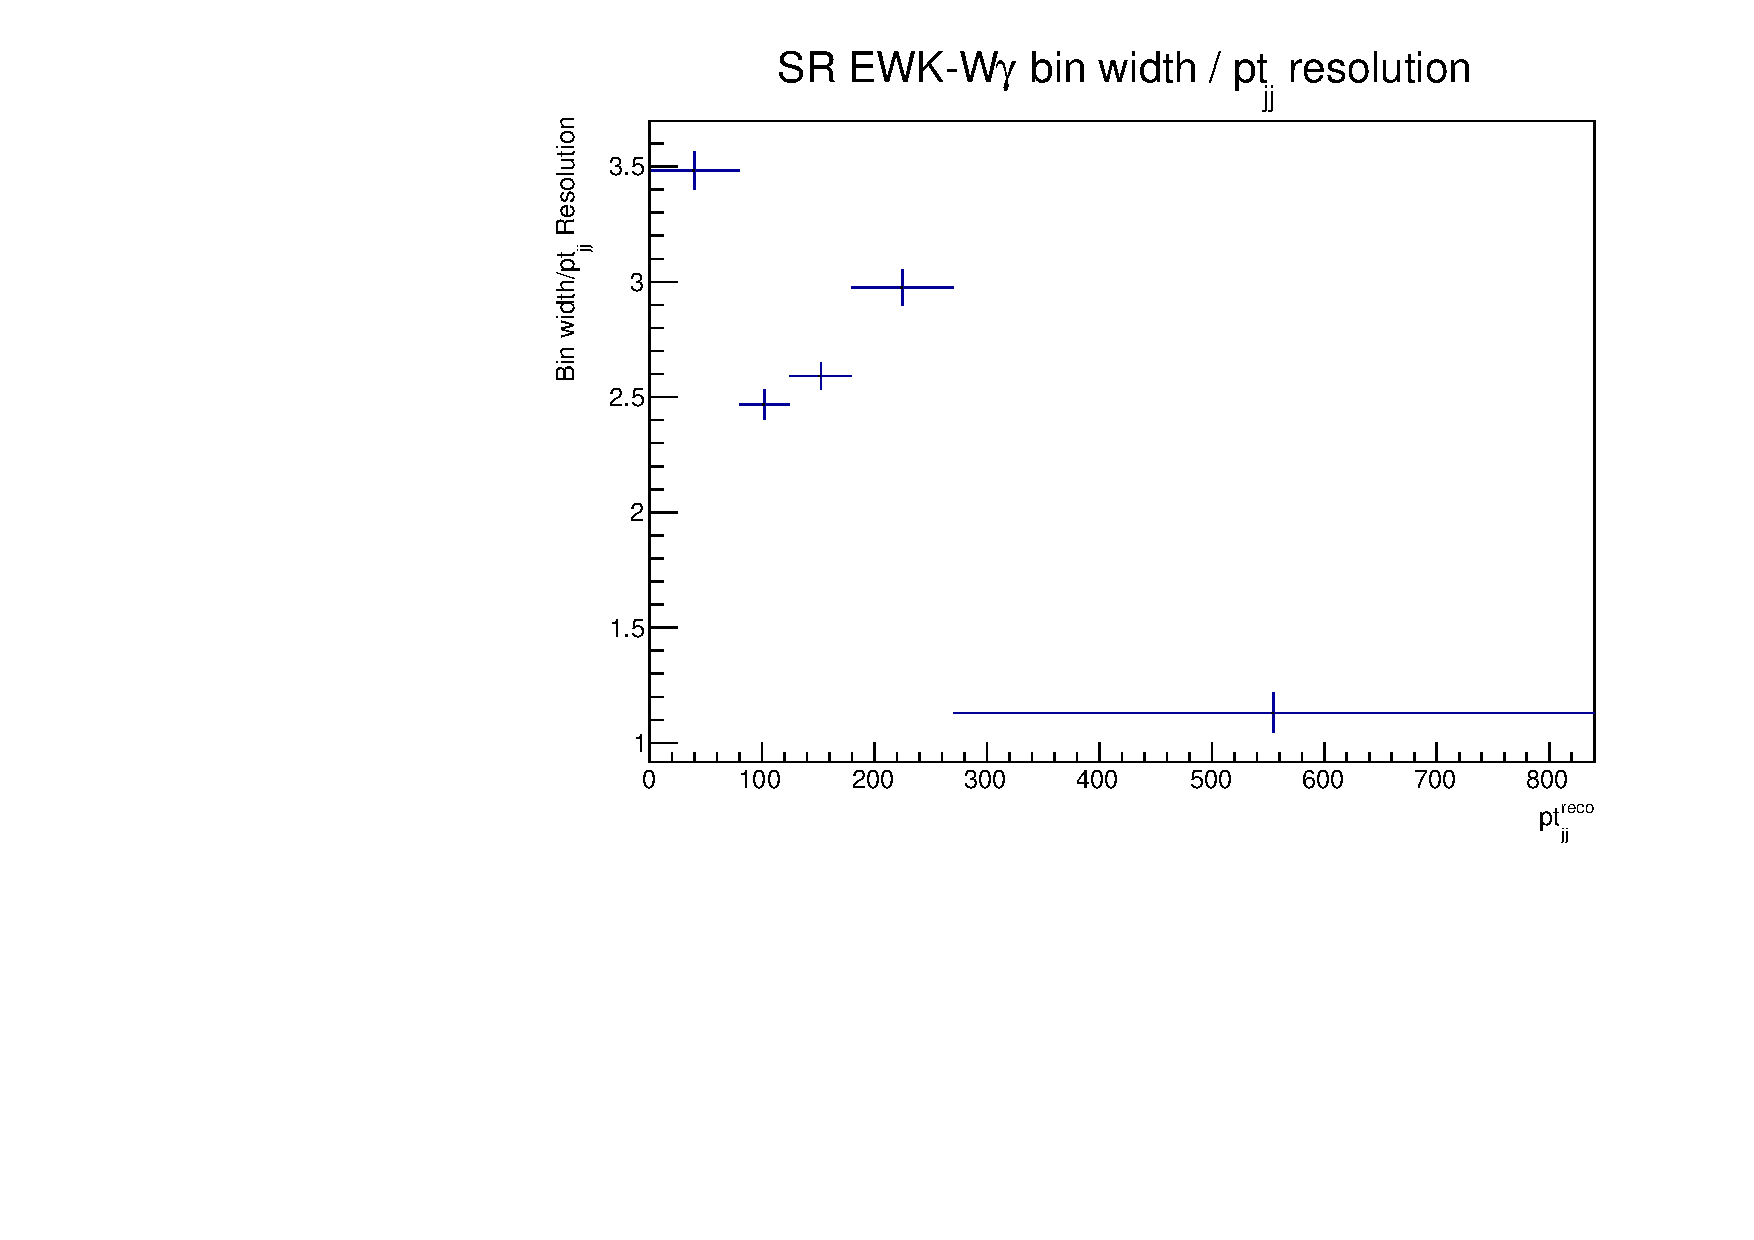
\includegraphics[width=\textwidth]{plots/diffx/binning/jj_pt_resolutions_rebin_SR.pdf}
    \caption{}
\end{subfigure}
\begin{subfigure}[b]{0.48\textwidth}
    \centering
    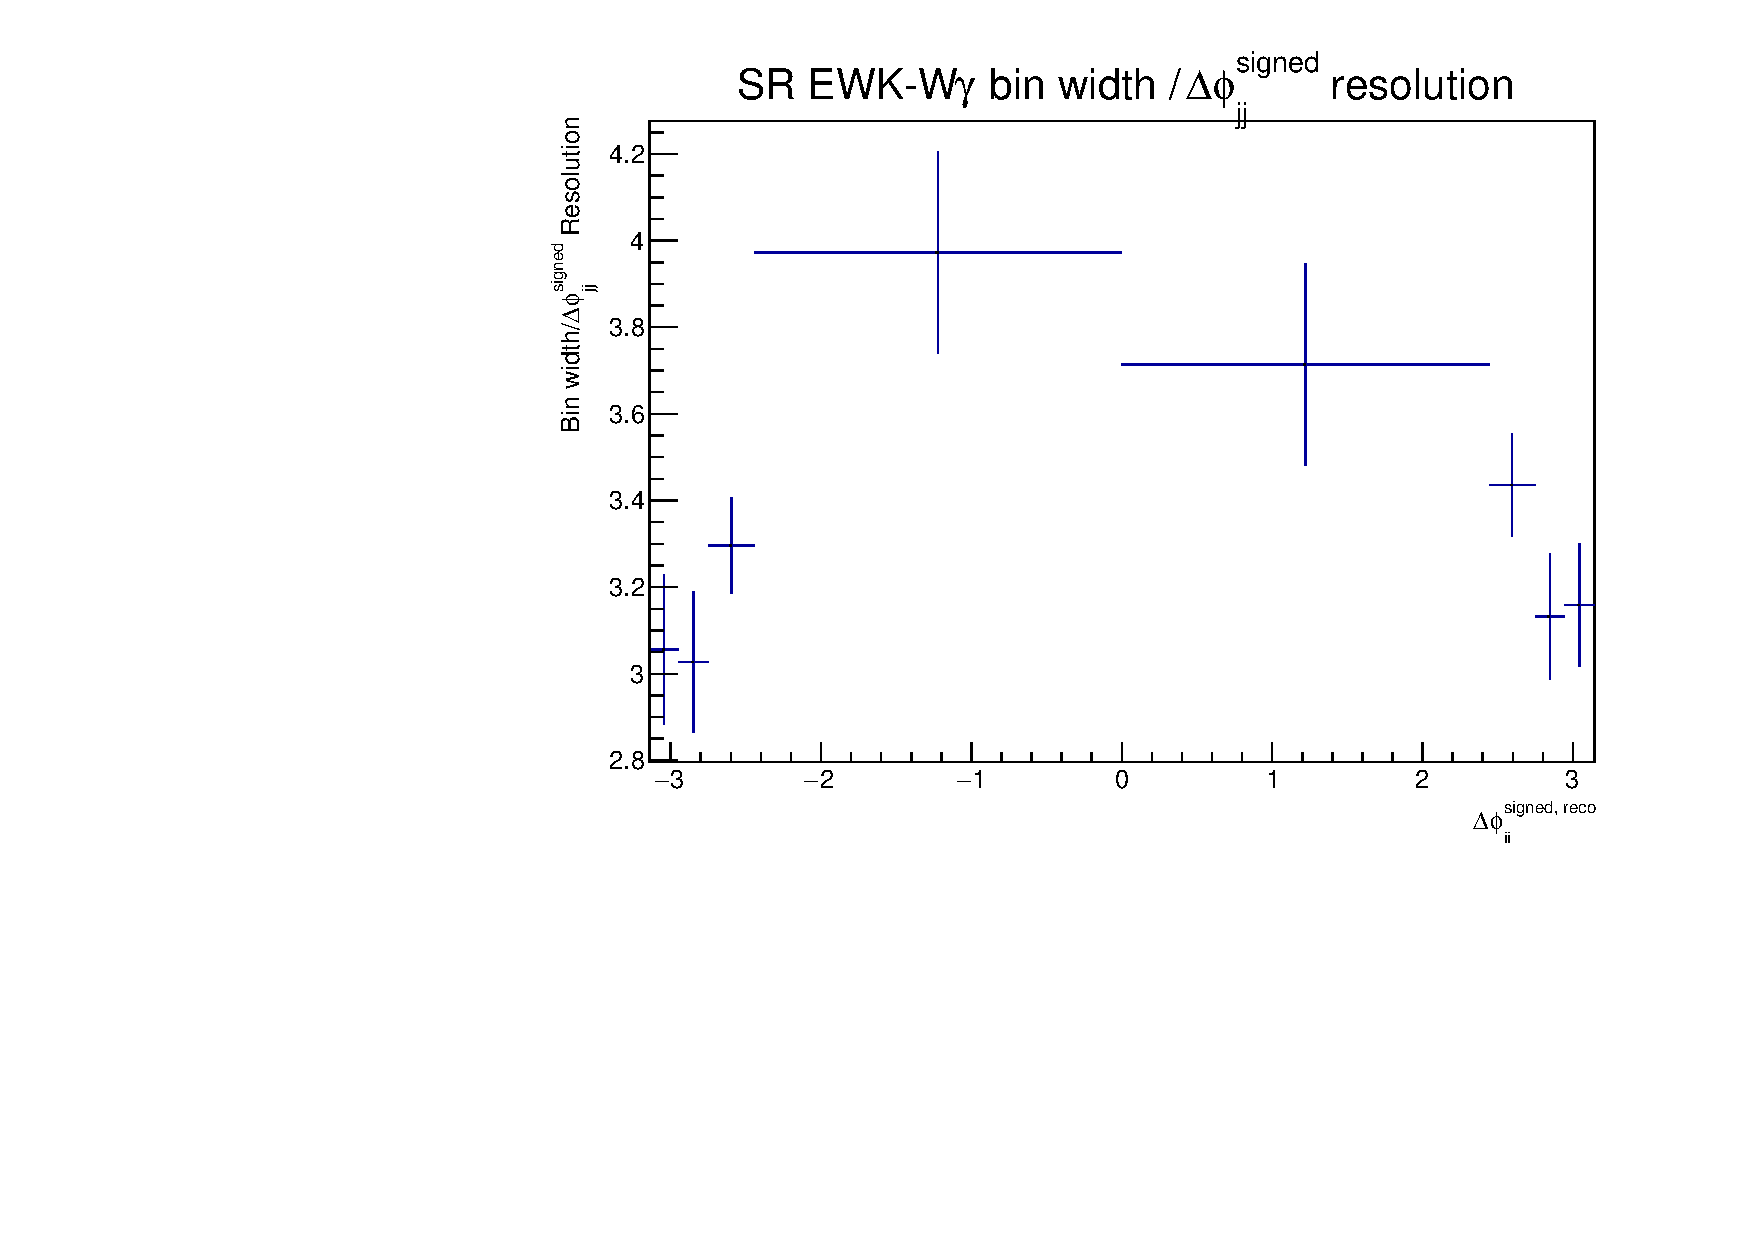
\includegraphics[width=\textwidth]{plots/diffx/binning/jj_dphi_signed_resolutions_rebin_SR.pdf}
    \caption{}
\end{subfigure}
\hfill
\begin{subfigure}[b]{0.48\textwidth}
    \centering
    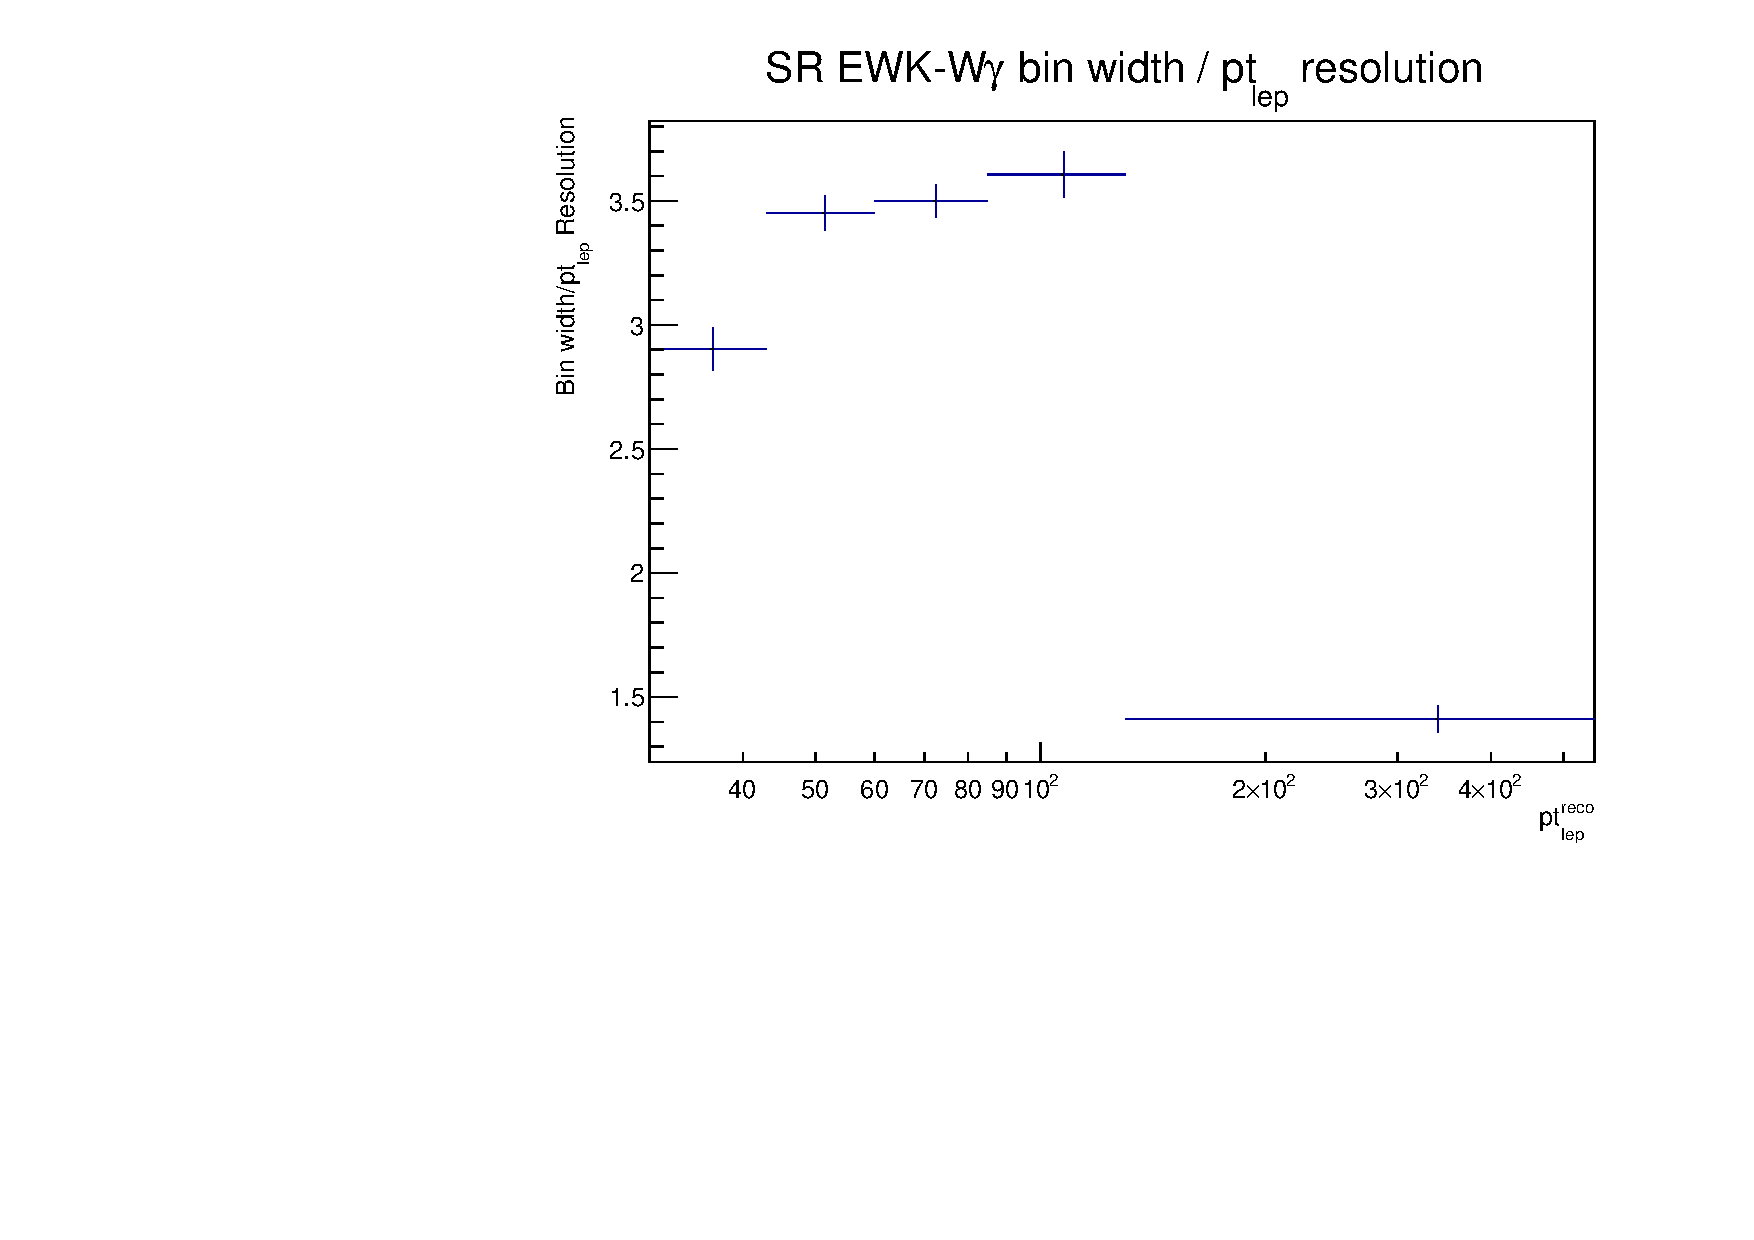
\includegraphics[width=\textwidth]{plots/diffx/binning/lep_pt_resolutions_rebin_SR.pdf}
    \caption{}
\end{subfigure}
\begin{subfigure}[b]{0.48\textwidth}
    \centering
    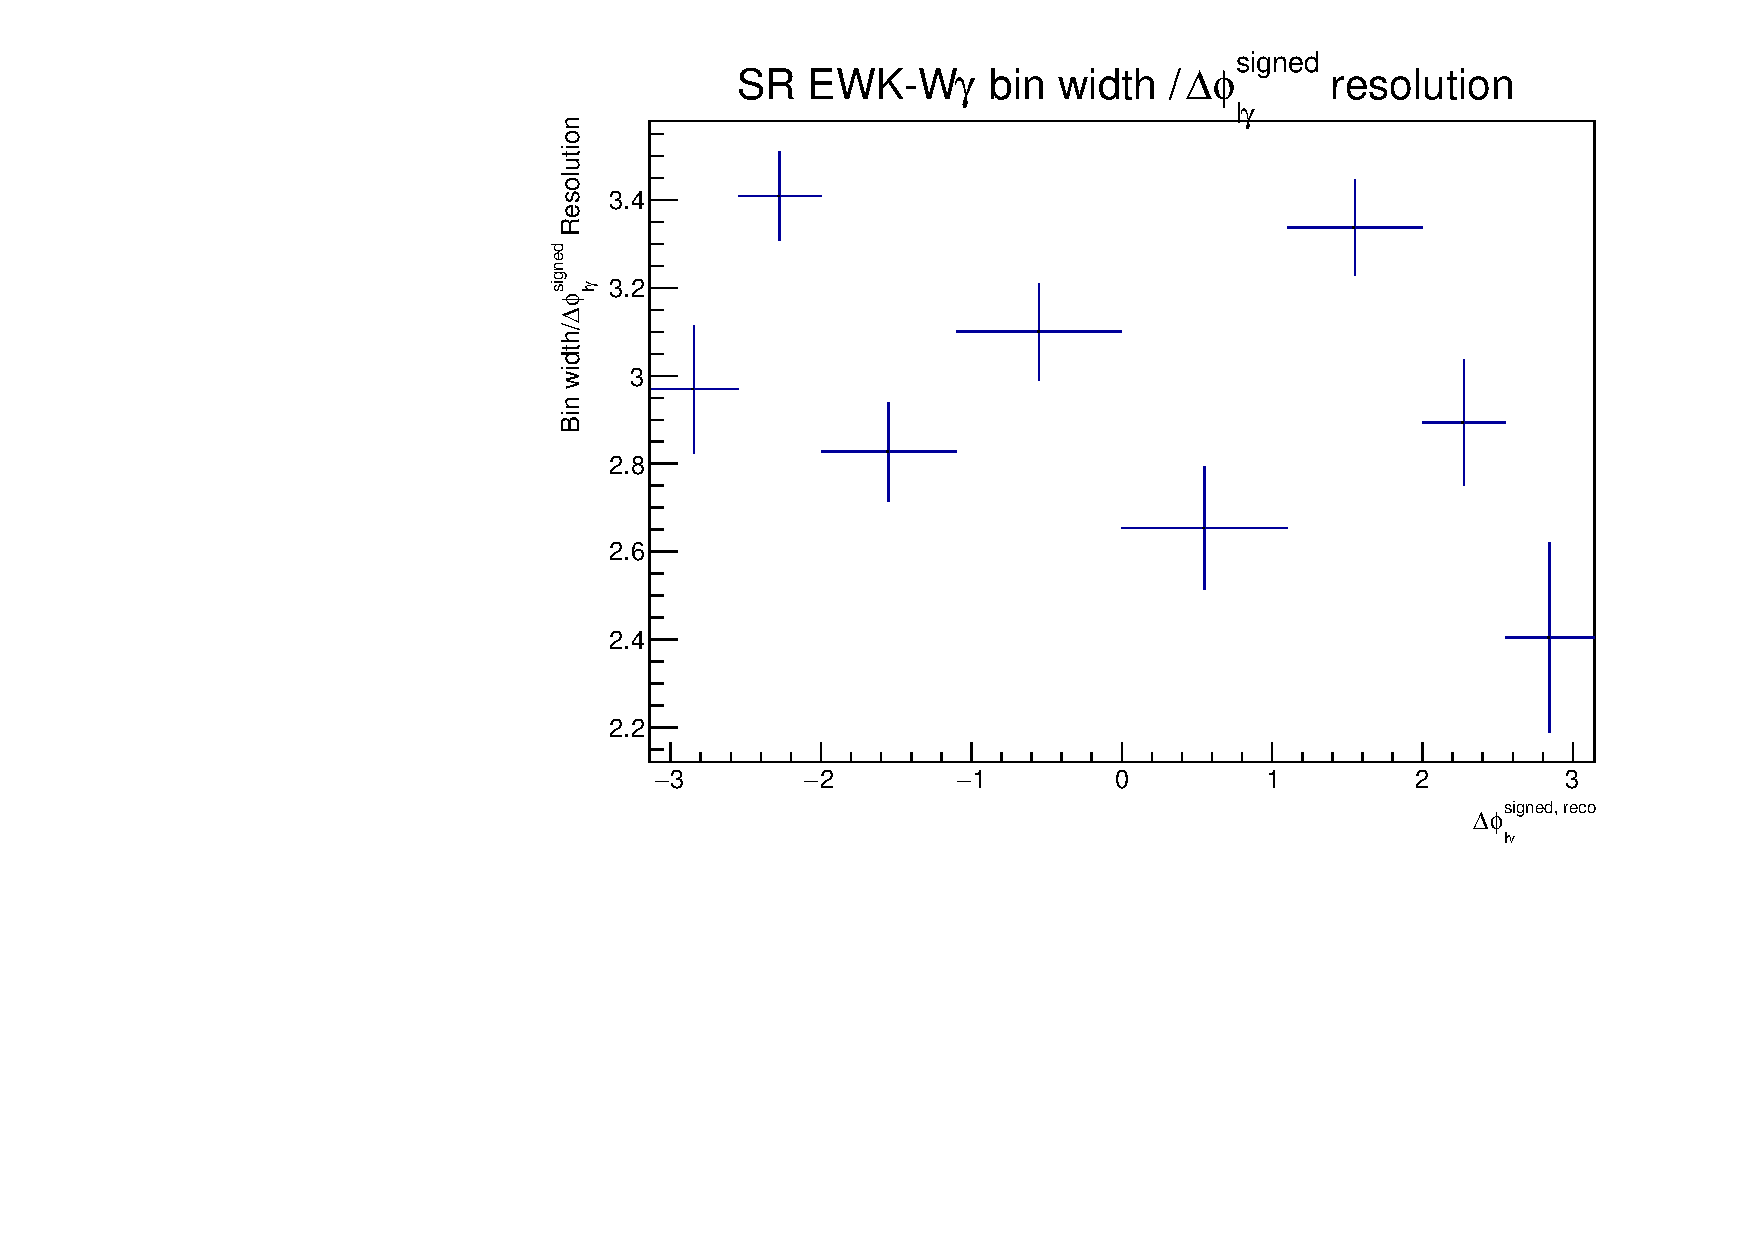
\includegraphics[width=\textwidth]{plots/diffx/binning/lepgam_dphi_signed_resolutions_rebin_SR.pdf}
    \caption{}
\end{subfigure}
\hfill
\begin{subfigure}[b]{0.48\textwidth}
    \centering
    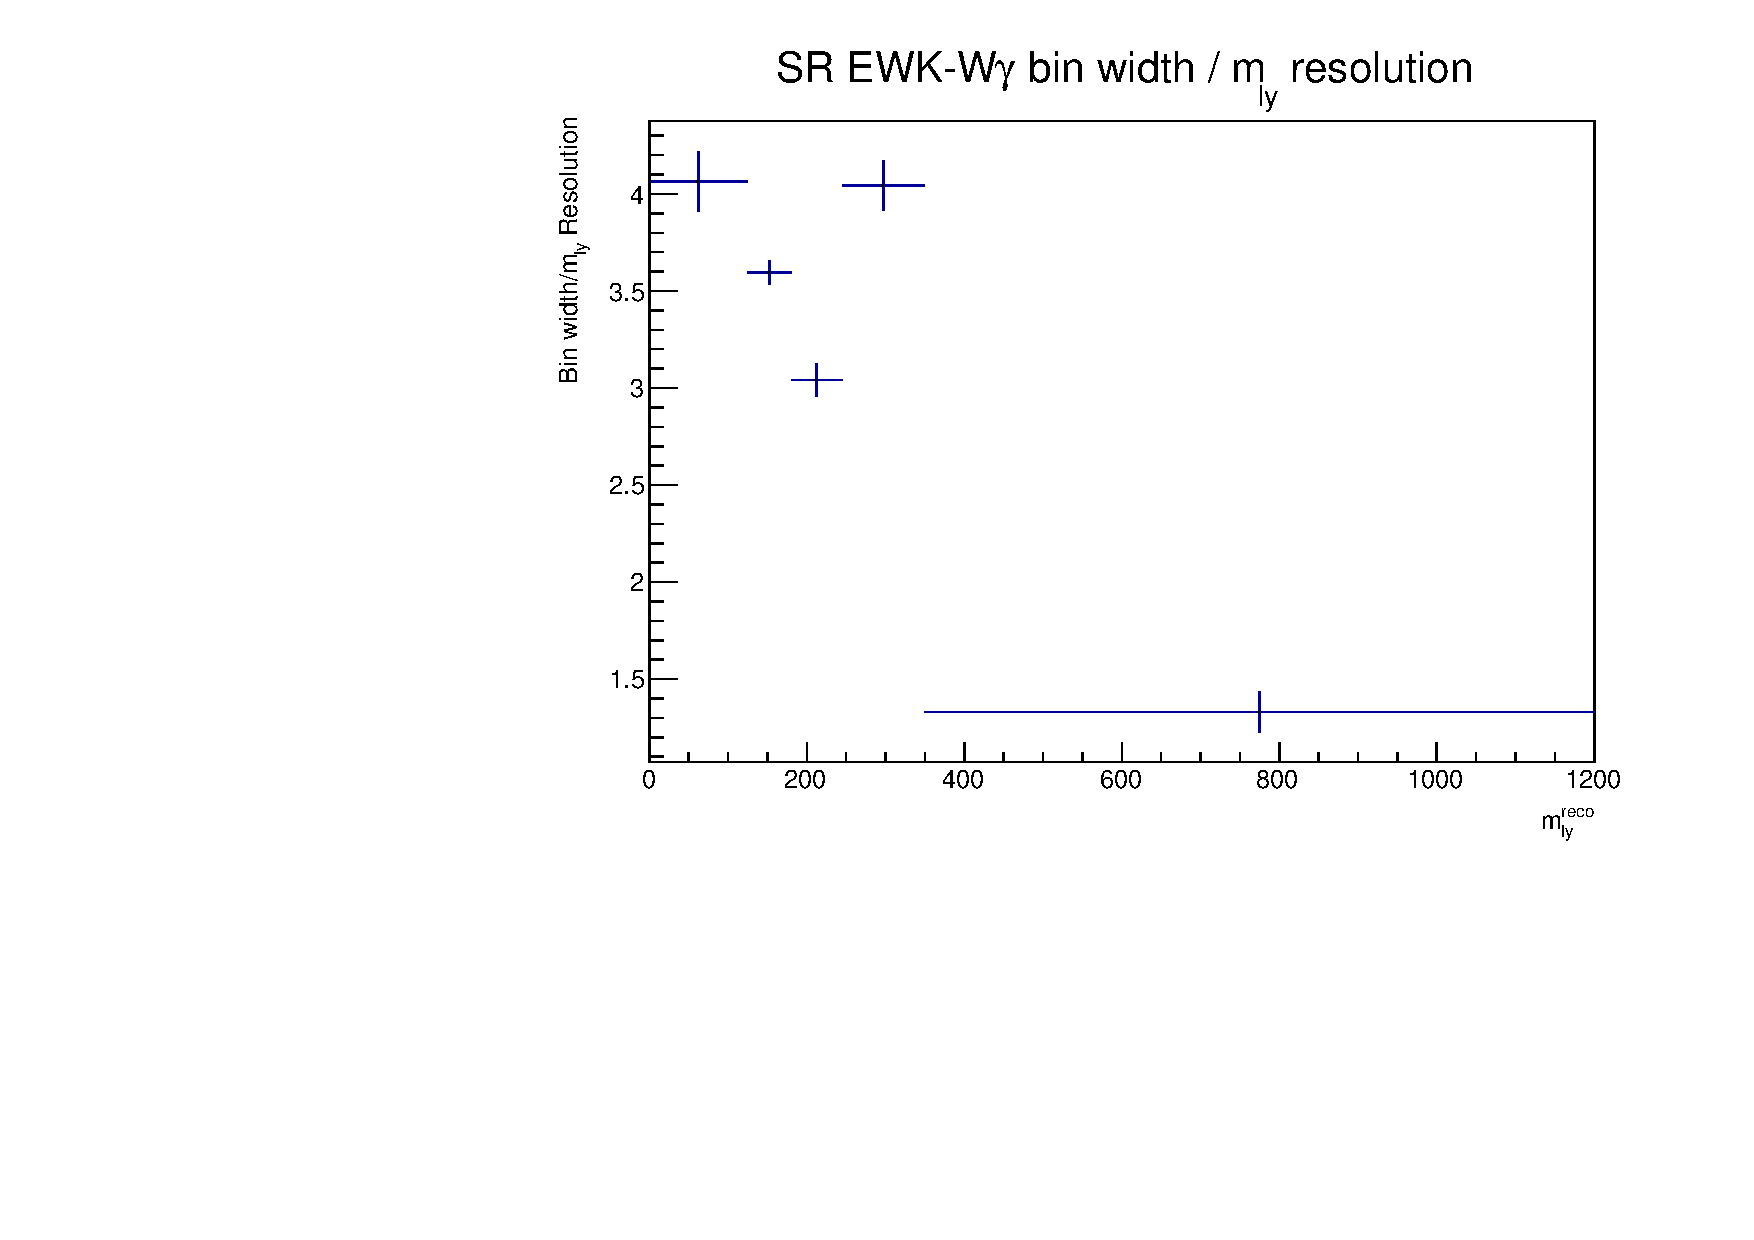
\includegraphics[width=\textwidth]{plots/diffx/binning/ly_m_resolutions_rebin_SR.pdf}
    \caption{}
\end{subfigure}
\caption{Reco bin width / resolution for each measured observable in the signal region for the \ewwy prediction. For all observables, the bin widths are consistent with passing the 2$\sigma$ threshold after ignoring the last bins of the kinematic observables.}\label{fig:vbswy:resolutionsrebin}
\end{figure}

The fits which lead to the resolution values shown in this plot can be seen in Figure \ref{fig:vbswy:resolutionmjj} for \mjj. For very large ranges such as the last bin of \mjj, \leppt, and \mly, the truth distribution is not well described by a Gaussian. This is simply an artifact of the bin range, and these bins therefore implicitly pass the $2\sigma$ requirement.

\begin{figure}[t]
\centering
\begin{subfigure}[b]{0.48\textwidth}
    \centering
    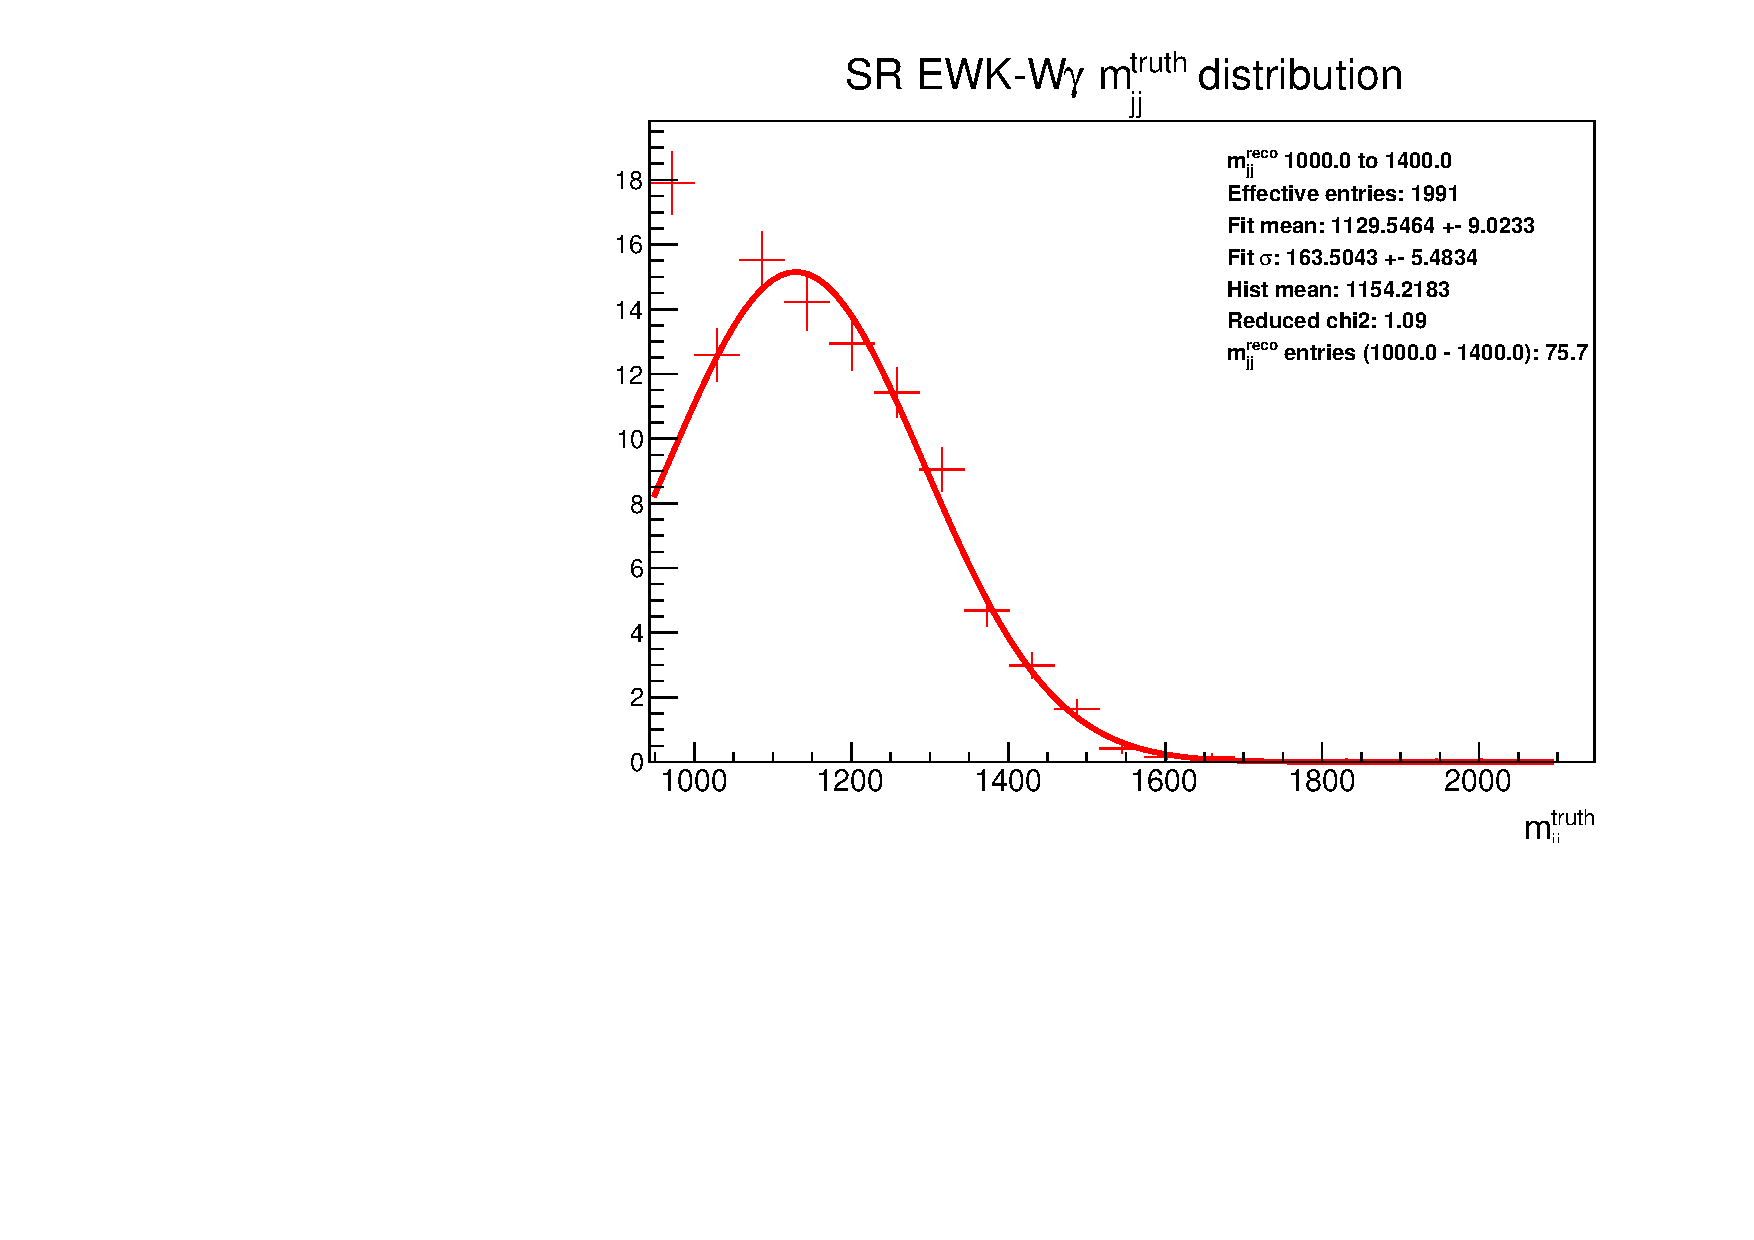
\includegraphics[width=\textwidth]{plots/diffx/binning/Gaussians/jj_m_bin1_SR.pdf}
    \caption{}
\end{subfigure}
\hfill
\begin{subfigure}[b]{0.48\textwidth}
    \centering
    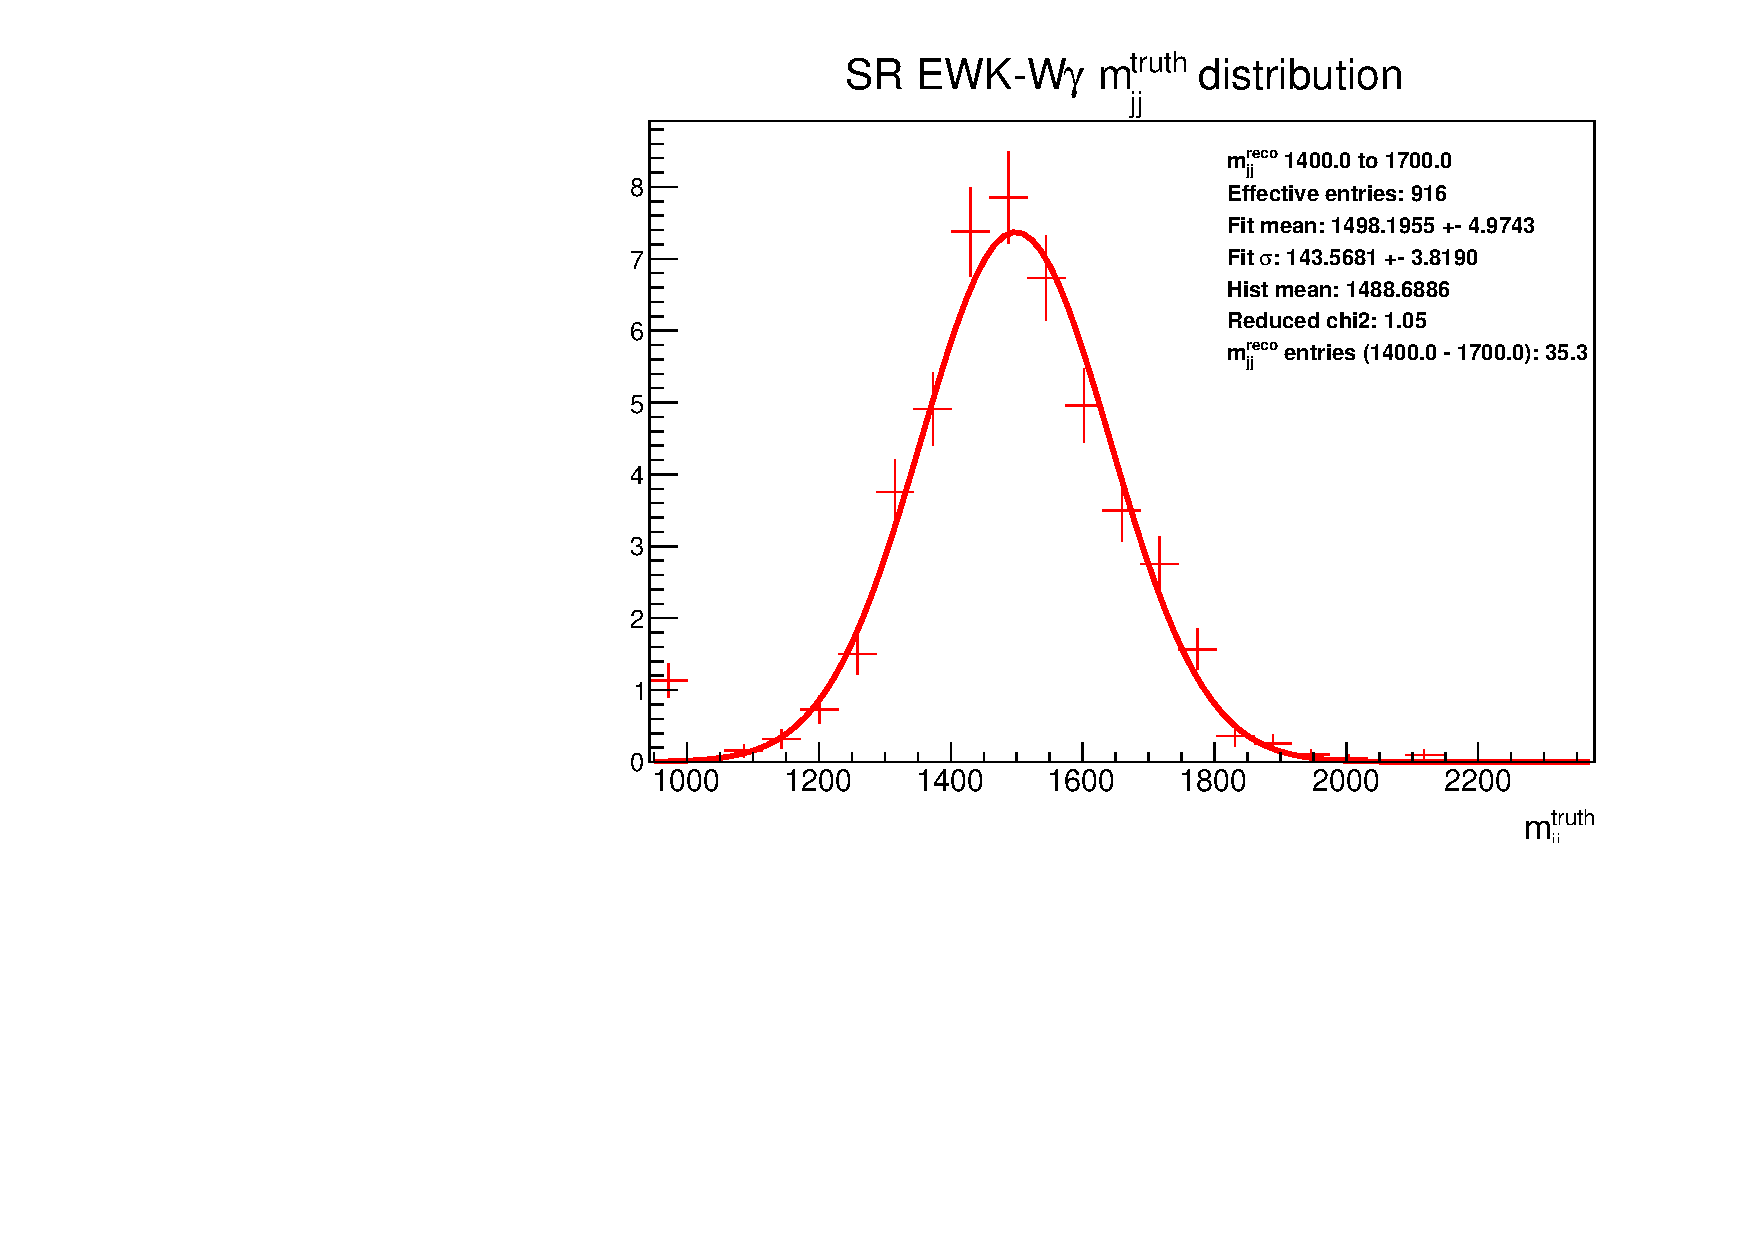
\includegraphics[width=\textwidth]{plots/diffx/binning/Gaussians/jj_m_bin2_SR.pdf}
    \caption{}
\end{subfigure}
\begin{subfigure}[b]{0.48\textwidth}
    \centering
    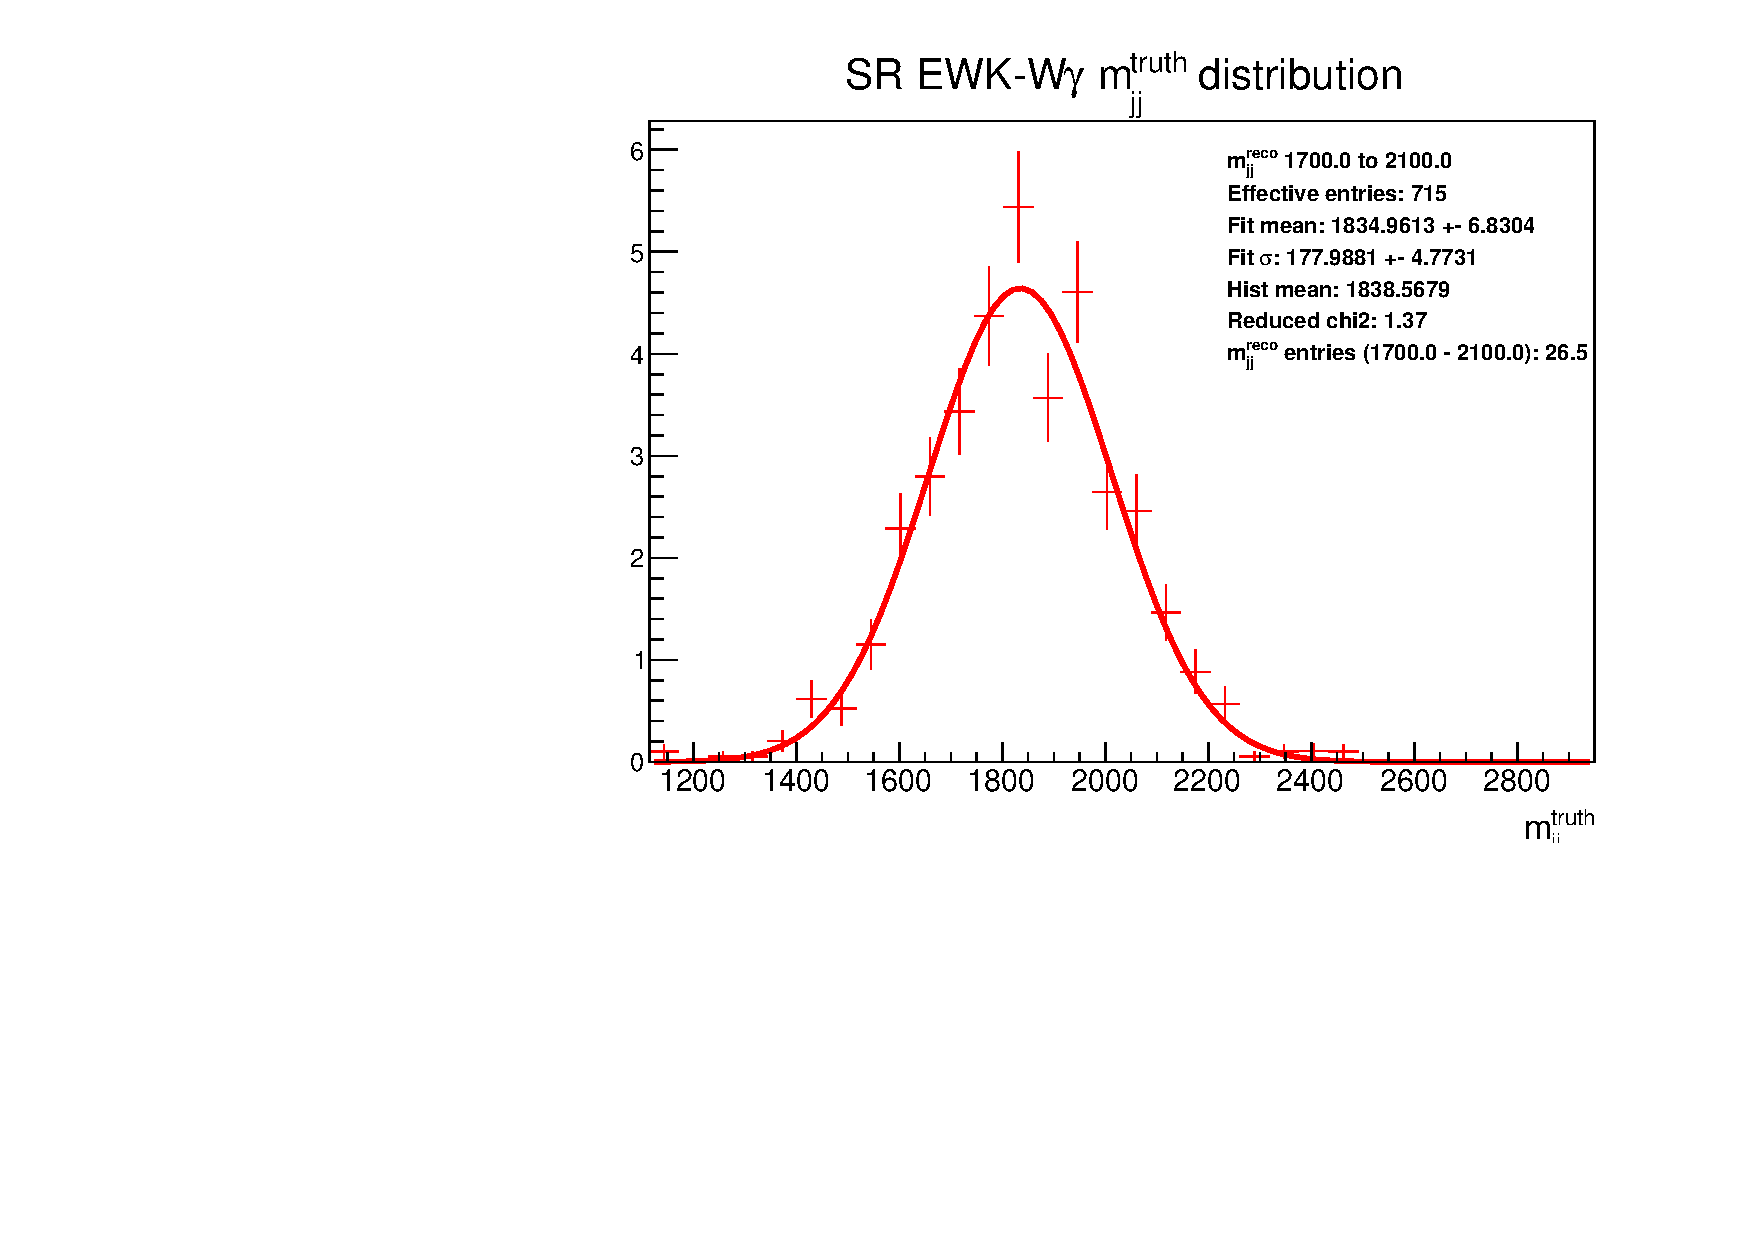
\includegraphics[width=\textwidth]{plots/diffx/binning/Gaussians/jj_m_bin3_SR.pdf}
    \caption{}
\end{subfigure}
\hfill
\begin{subfigure}[b]{0.48\textwidth}
    \centering
    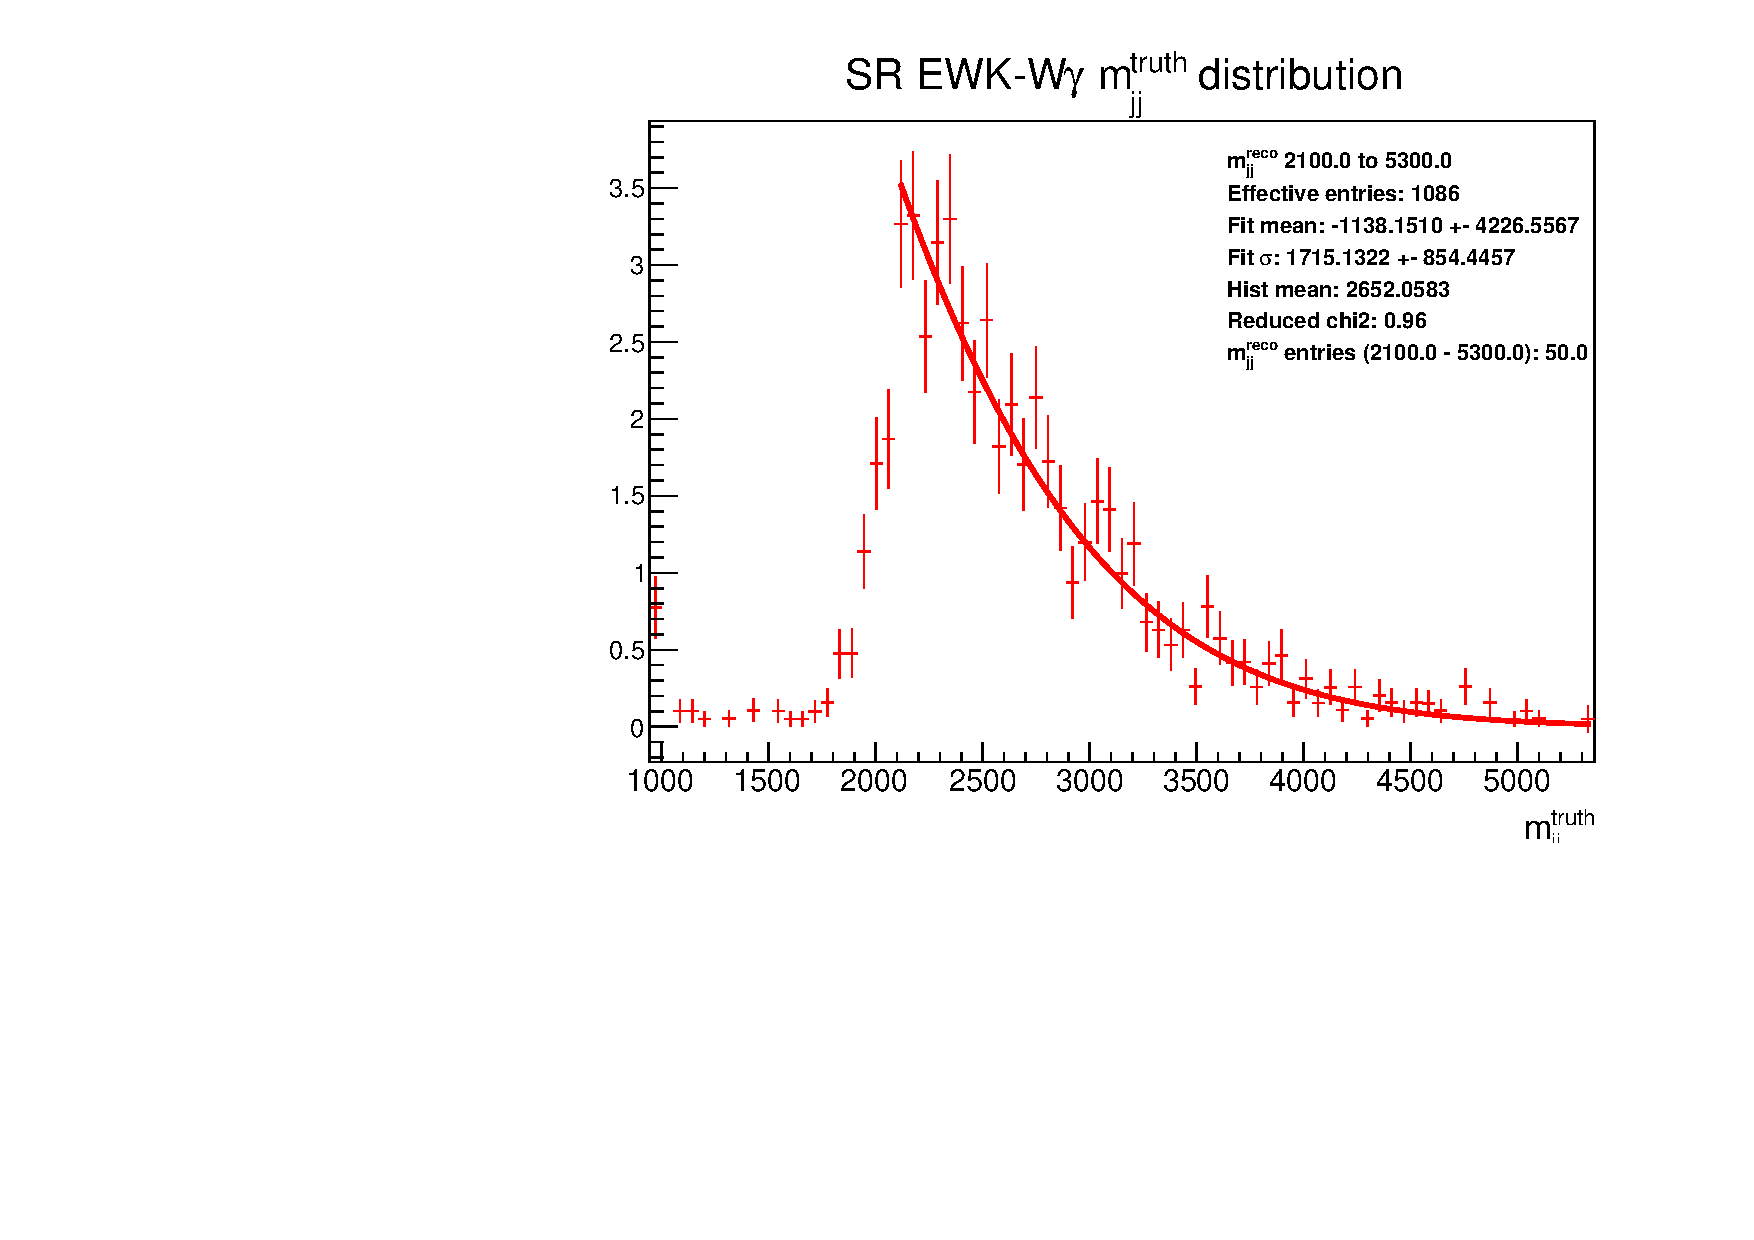
\includegraphics[width=\textwidth]{plots/diffx/binning/Gaussians/jj_m_bin4_SR.pdf}
    \caption{}
\end{subfigure}
\caption{Resolution fits for \mjj. The first three bins are well described by a Gaussian distribution as the truth distribution is relatively uniform in these bins. The non-Gaussian shape in the last bin is an artifact of the large reco-variable range, therefore the last bin implicitly passes the 2$\sigma$ requirement. The error on the fit parameters are defined as the change in the parameter value required to change the chi-squared value by 1 \cite{VBSWy:minuit}.\label{fig:vbswy:resolutionmjj}}
\end{figure}

%\clearpage
\section{Symmetrising of the \lepgamdphi and \jjdphi Templates\label{sec:vbswy:symdphi}}

Under the assumption of the standard model, the azimuthal separation of two objects is independent of the rapidity ordering, and any asymmetry would be an indication of CP violation. Furthermore, the ATLAS detector is symmetric in $\phi$, and therefore there is no a-priori reason for the fit templates to be asymmetric. In light of this, the possibility of symmetrising the fit templates of the angular observables around $\Delta\phi=0$ is explored.

To test whether it is valid to symmetrise the \lepgamdphi and \jjdphi templates, the data are plotted for these observables in the control regions, this is shown in Figure \ref{fig:data_dphi}. From this figure it is evident that the data are consistent with a symmetric distribution within statistical uncertainties. Therefore the Asimov dataset, data-driven fakes estimates and MC templates are all symmetrised for \lepgamdphi and \jjdphi prior to performing the likelihood fit. The observed data are left un-symmetrised. The benefits of this prescription are that the statistical precision each bin is then improved by a factor of $\sqrt{2}$ and that simulated events with large event weights are less likely to skew the likelihood fit results. 

\begin{figure}[htpb]
  \centering
  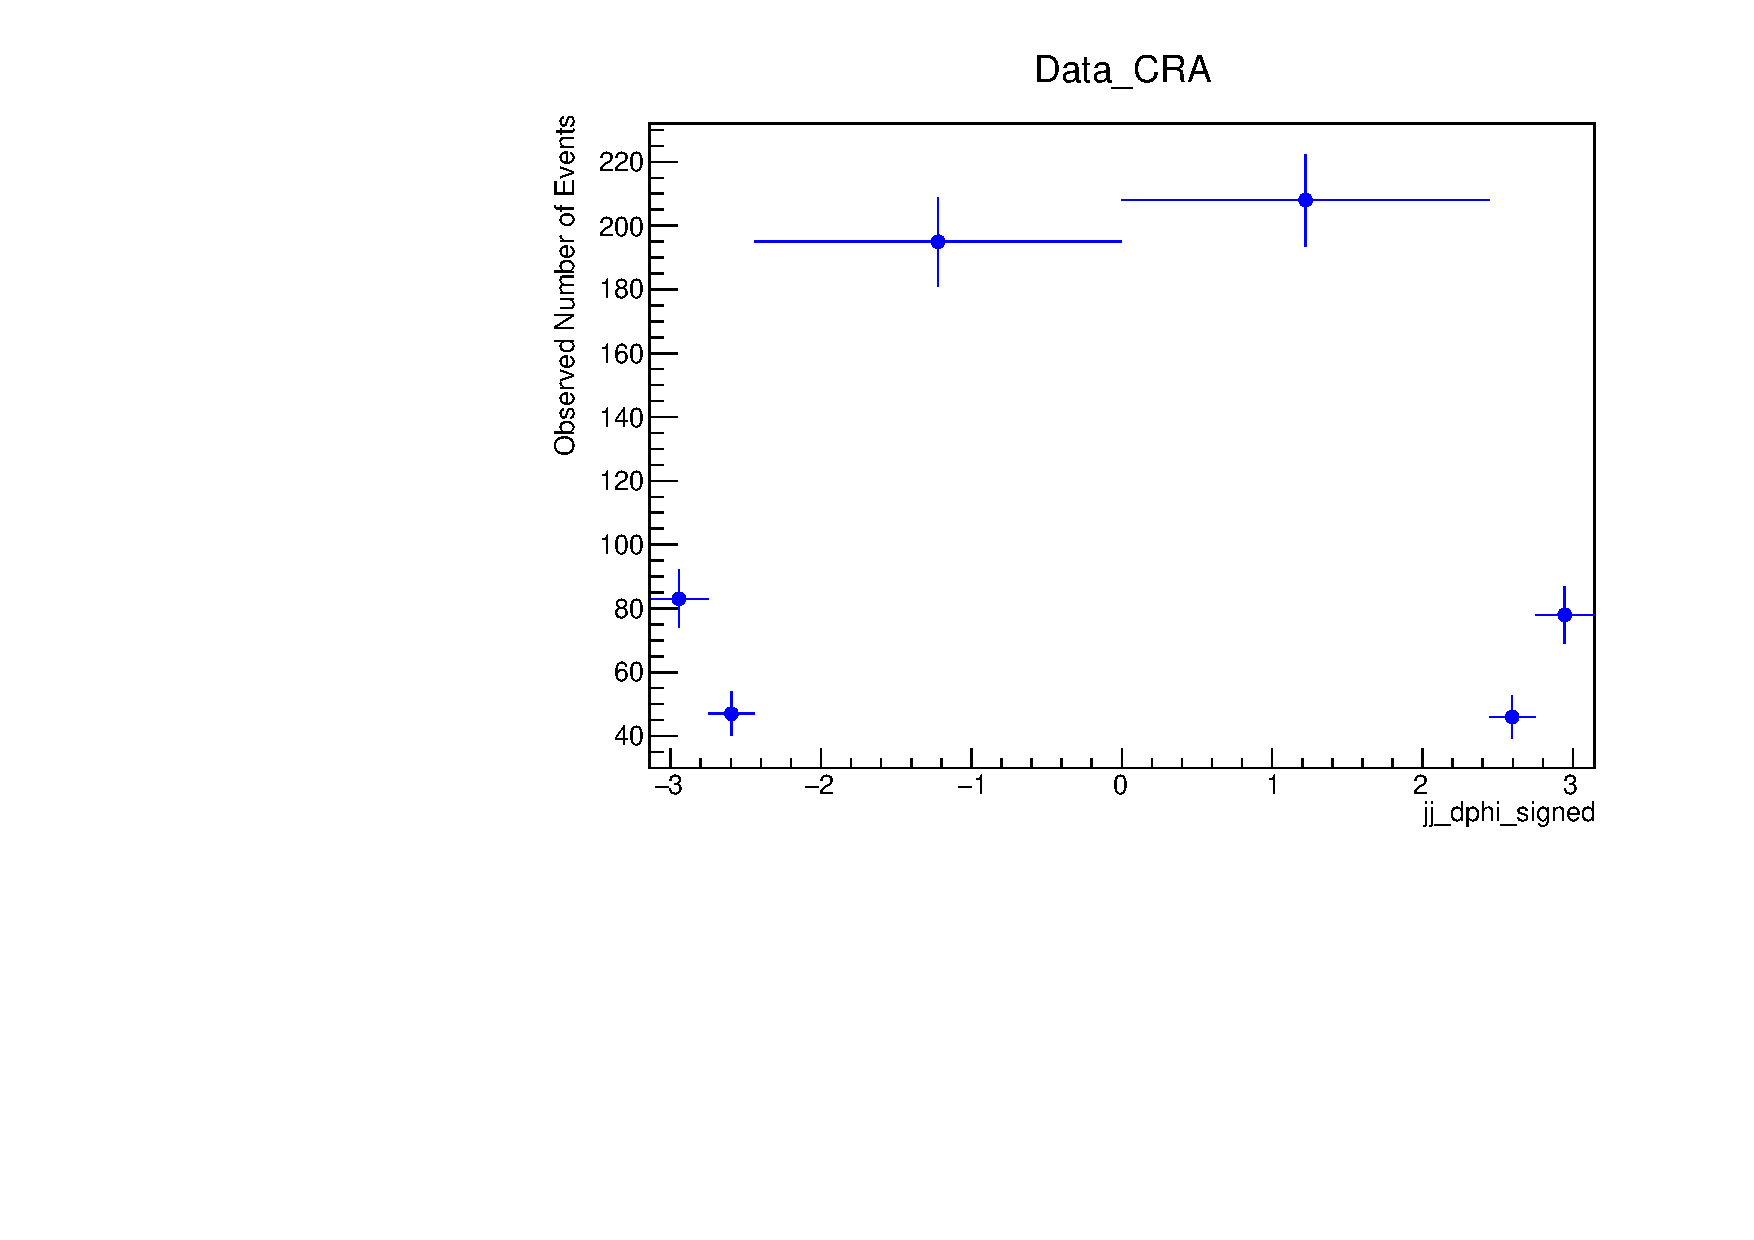
\includegraphics[width=0.48\textwidth]{plots/diffx/Data_CRA_jj_dphi_signed.pdf}
  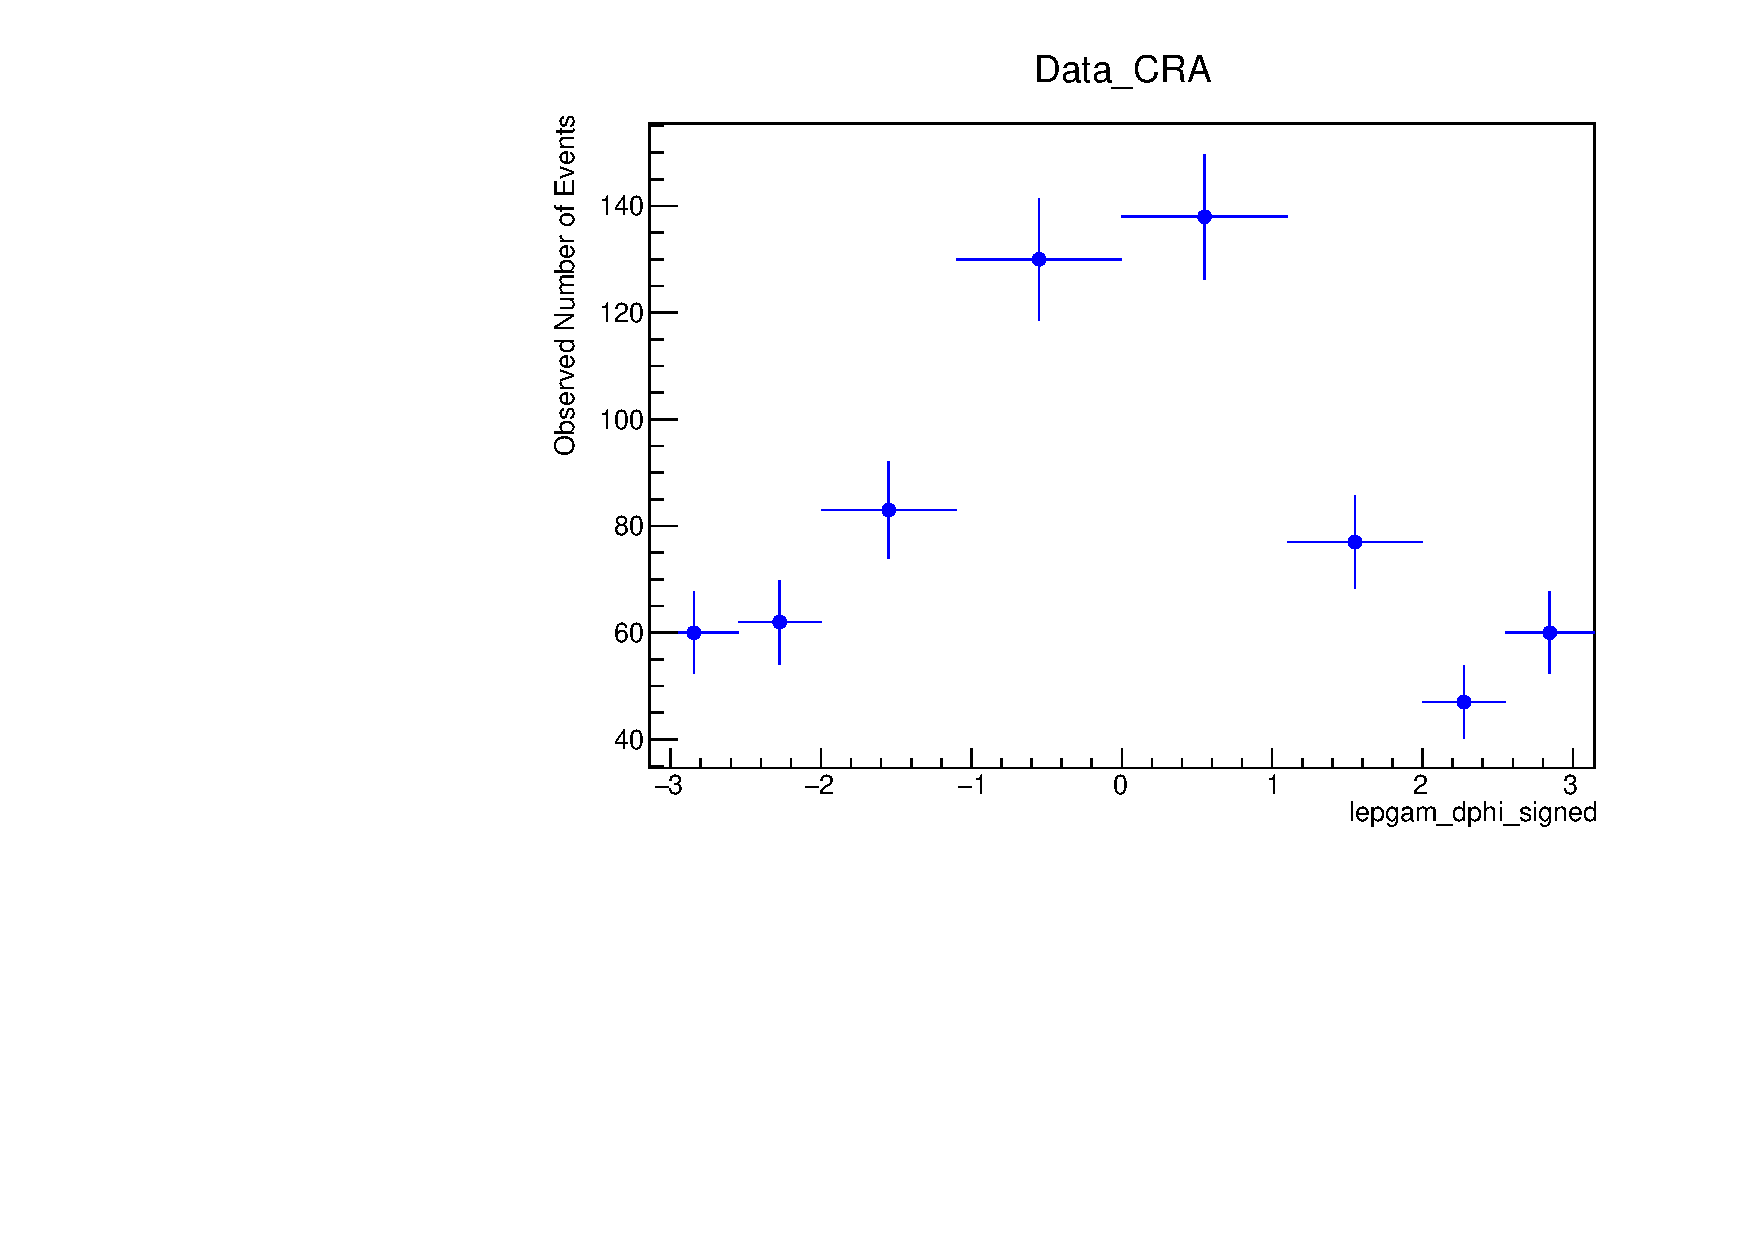
\includegraphics[width=0.48\textwidth]{plots/diffx/Data_CRA_lepgam_dphi_signed.pdf}
  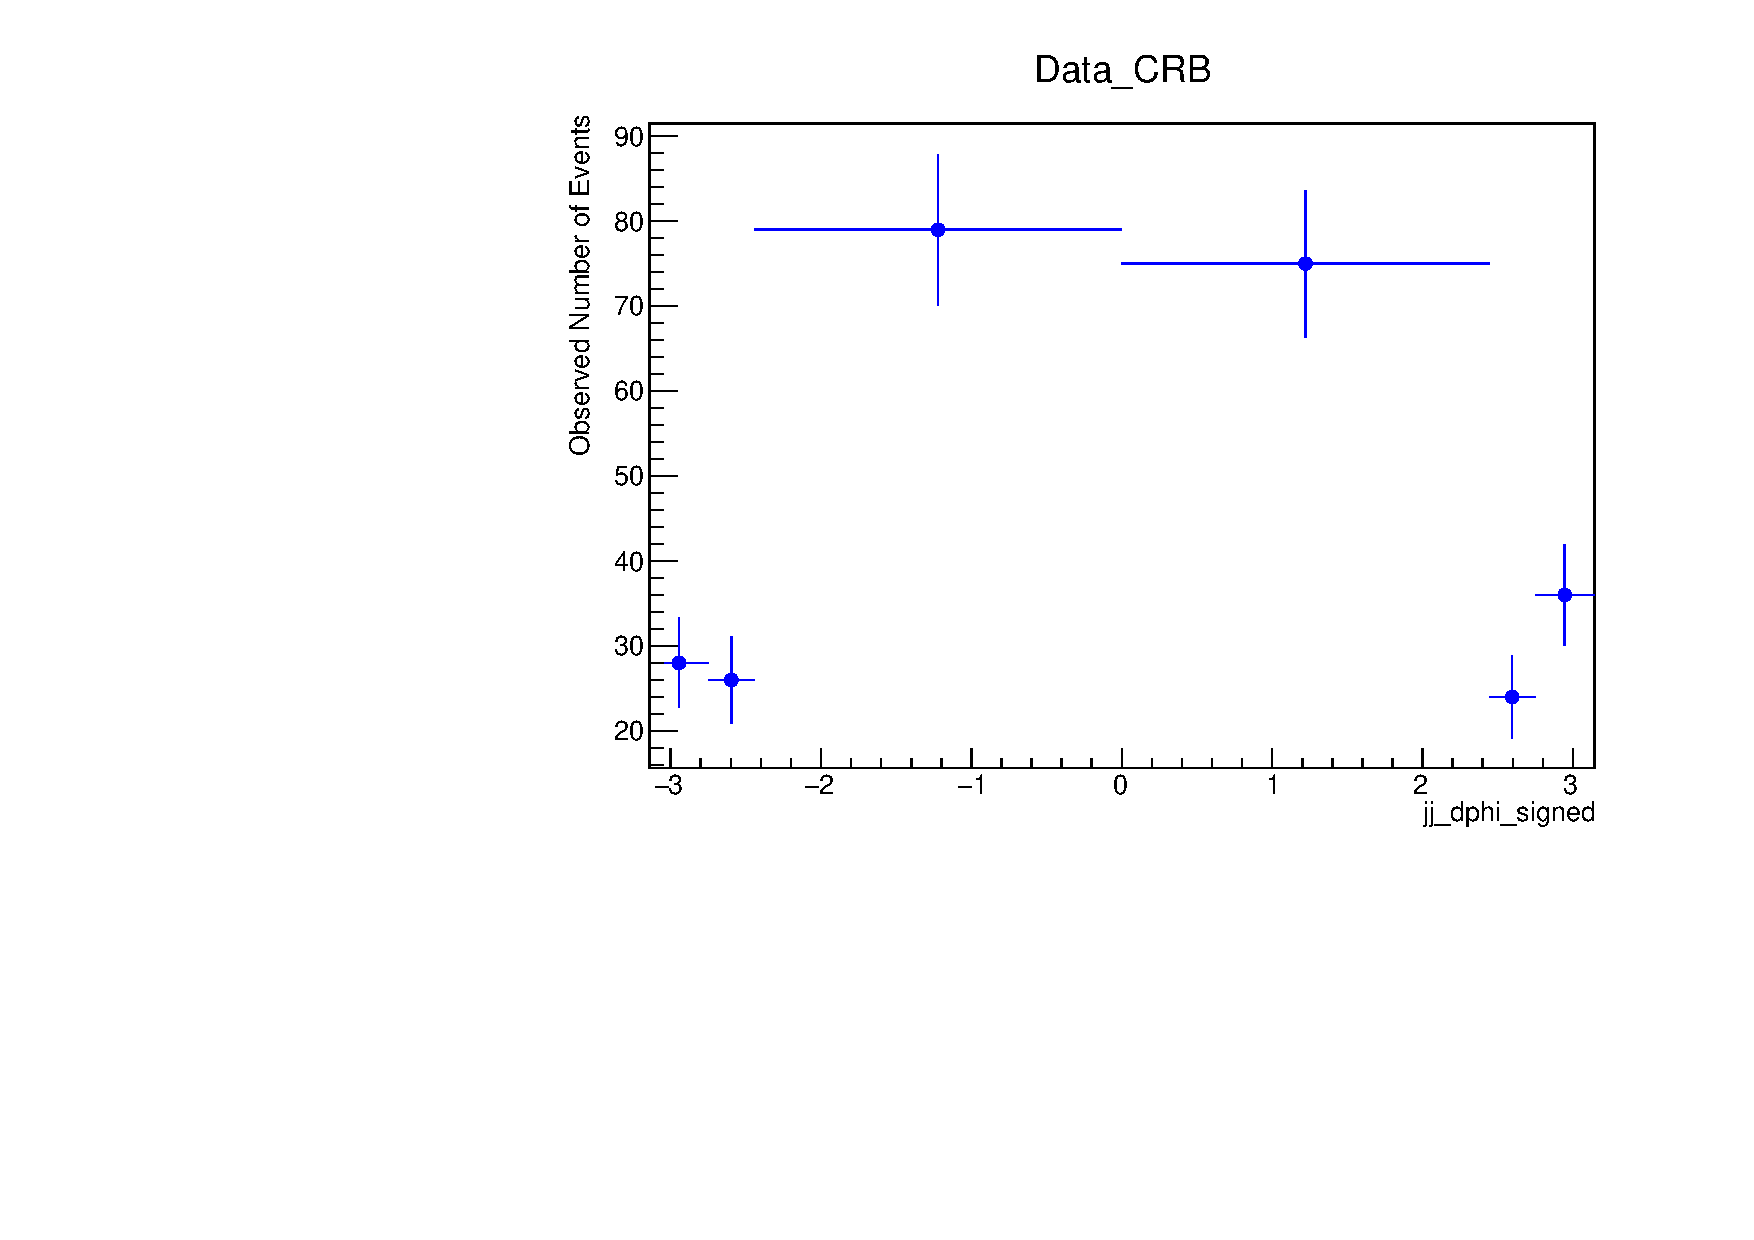
\includegraphics[width=0.48\textwidth]{plots/diffx/Data_CRB_jj_dphi_signed.pdf}
  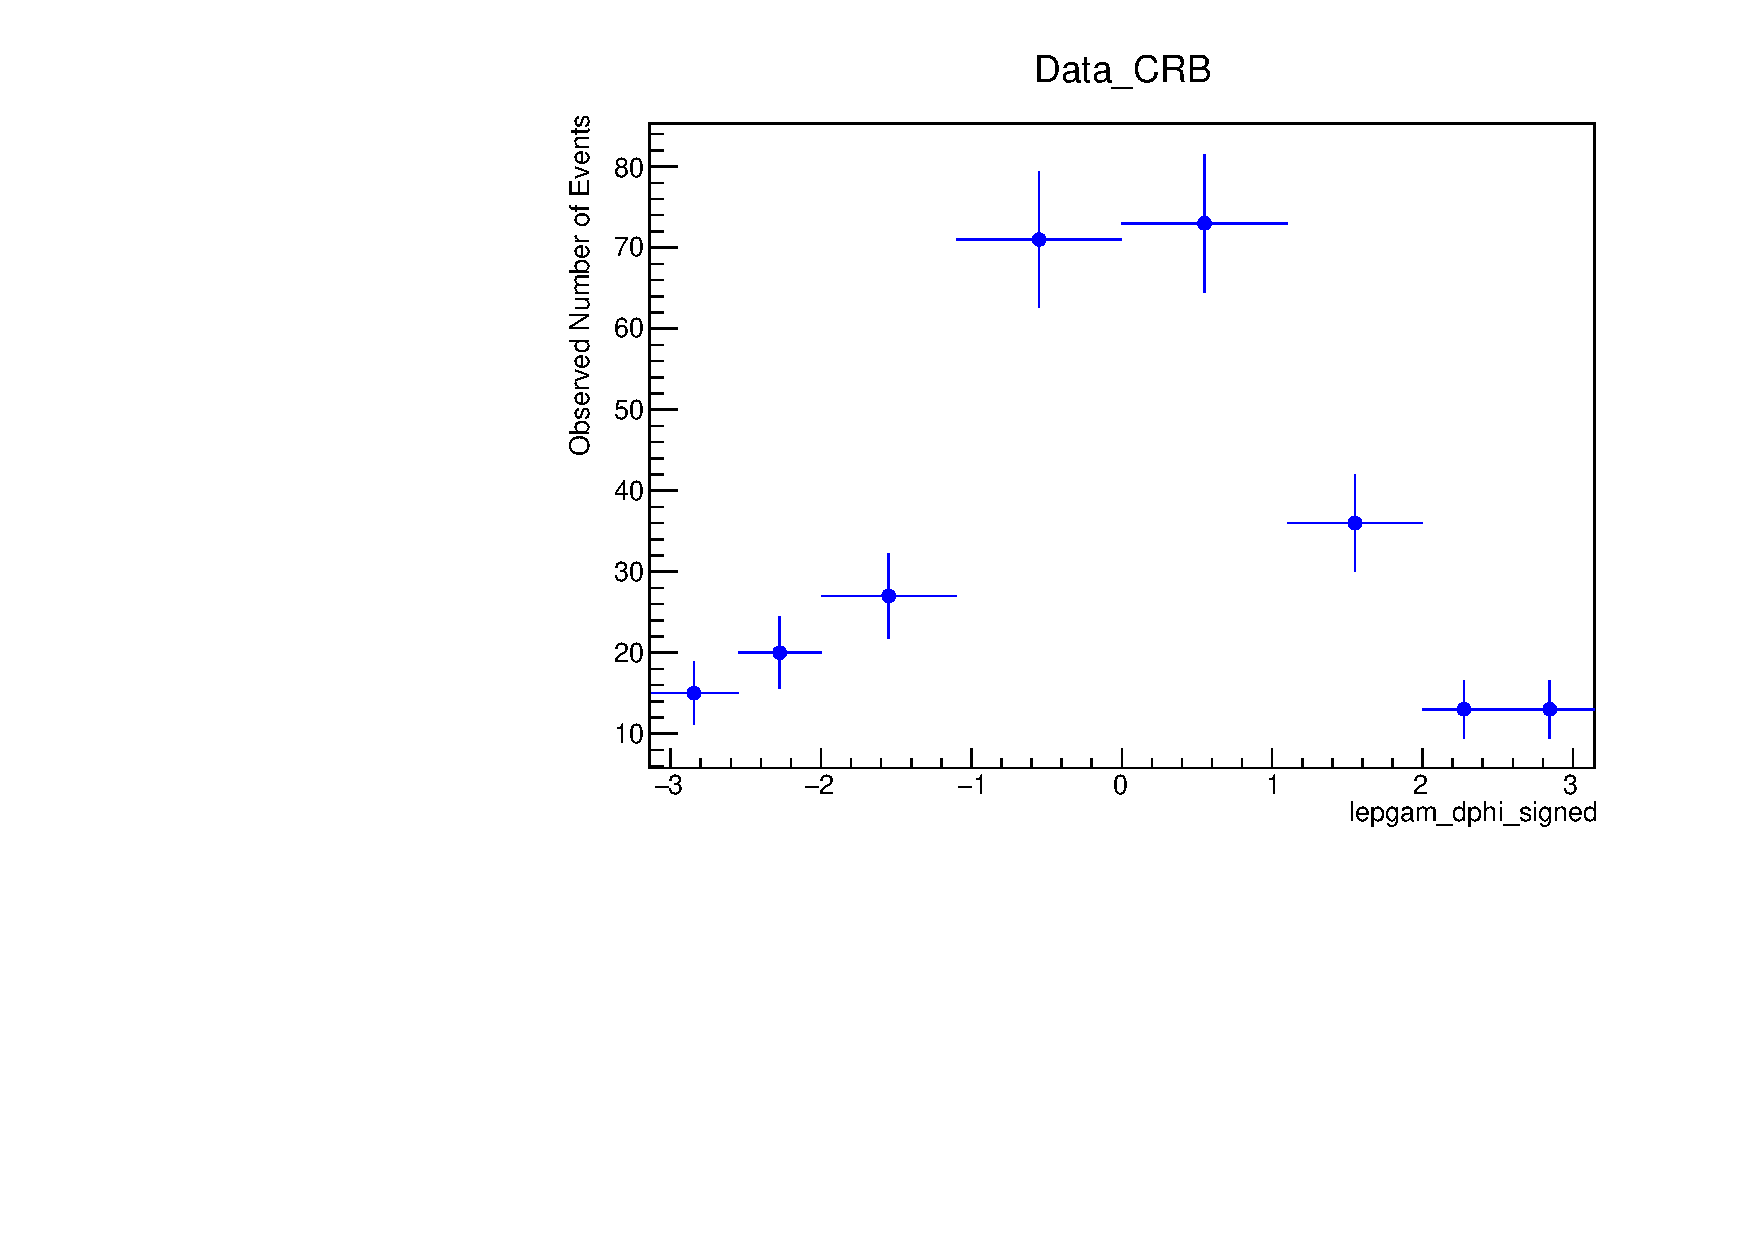
\includegraphics[width=0.48\textwidth]{plots/diffx/Data_CRB_lepgam_dphi_signed.pdf}
  \subfloat[Observed \jjdphi events]{%
    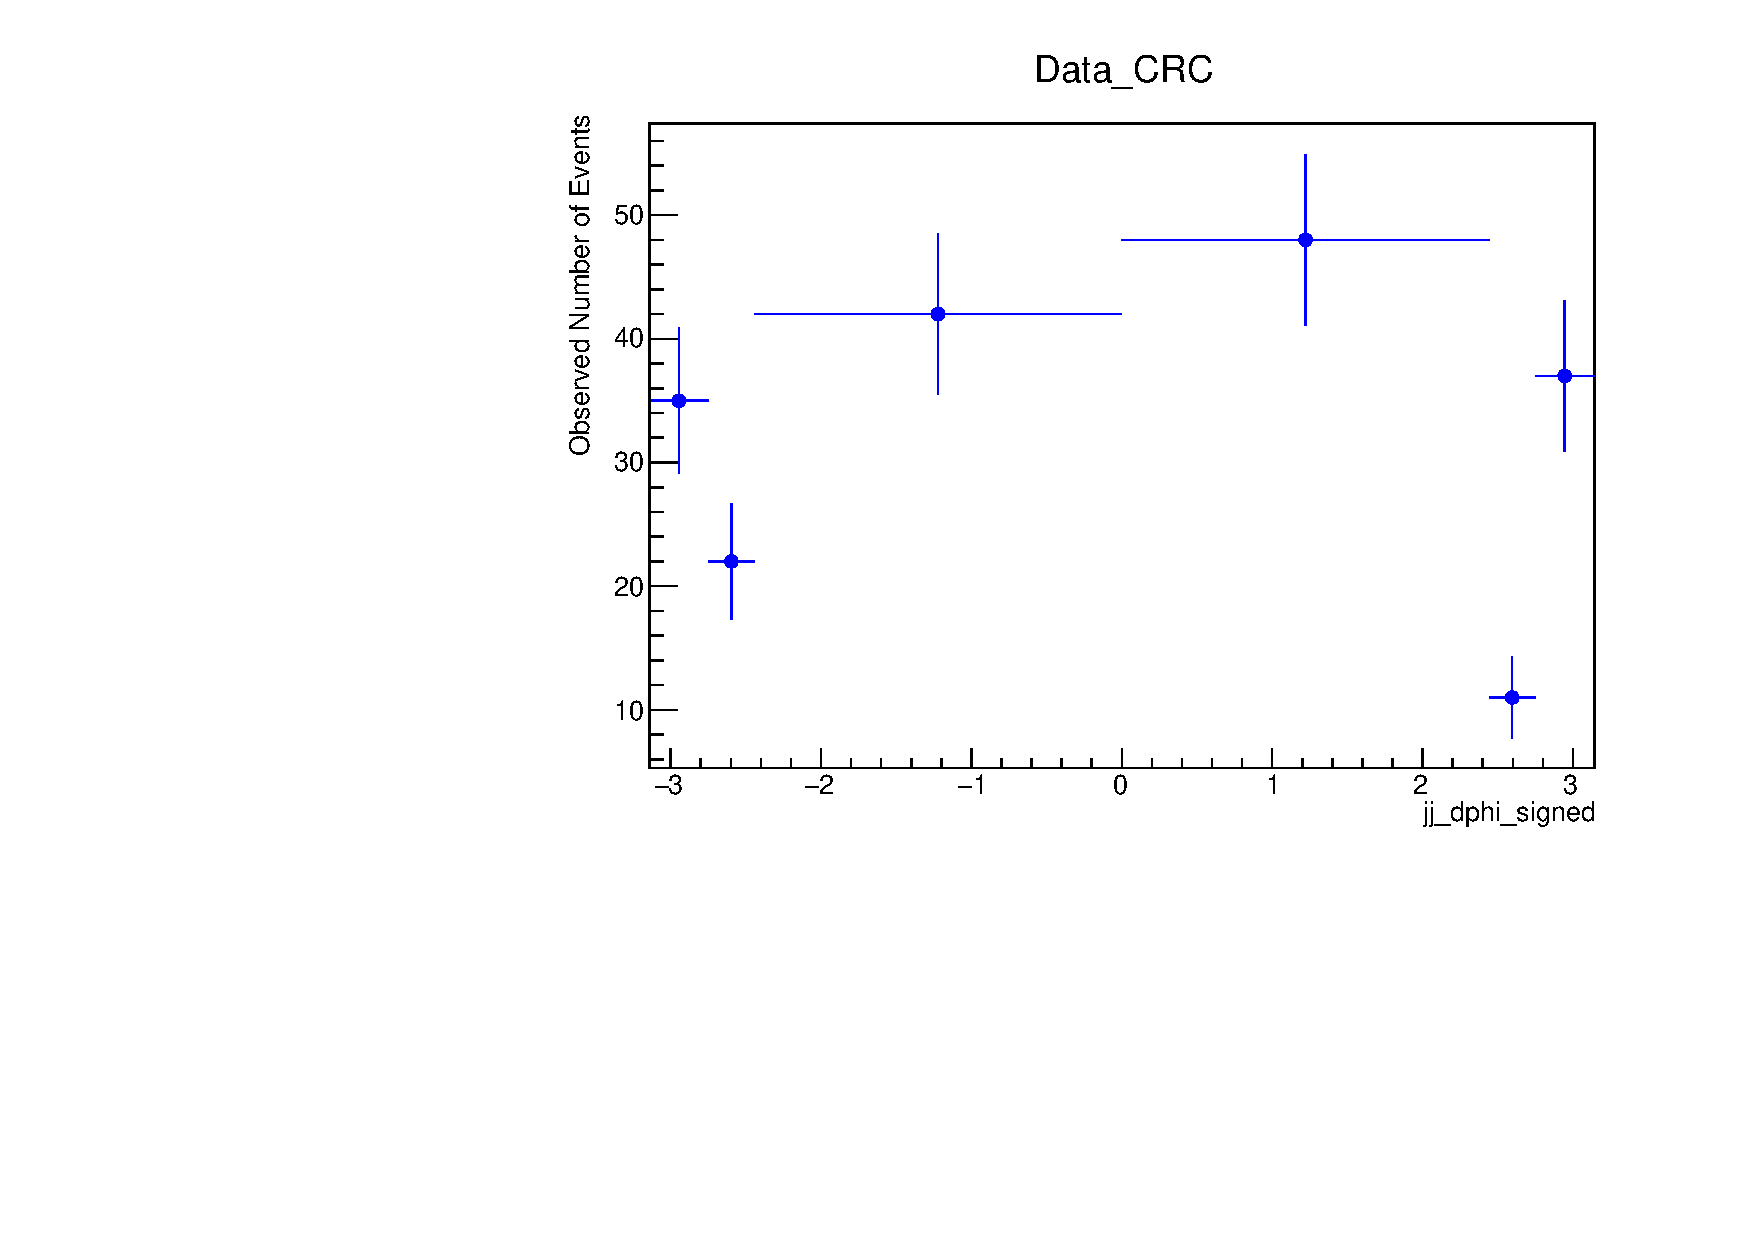
\includegraphics[width=0.48\textwidth]{plots/diffx/Data_CRC_jj_dphi_signed.pdf}
  }
  \subfloat[Observed \lepgamdphi events]{%
    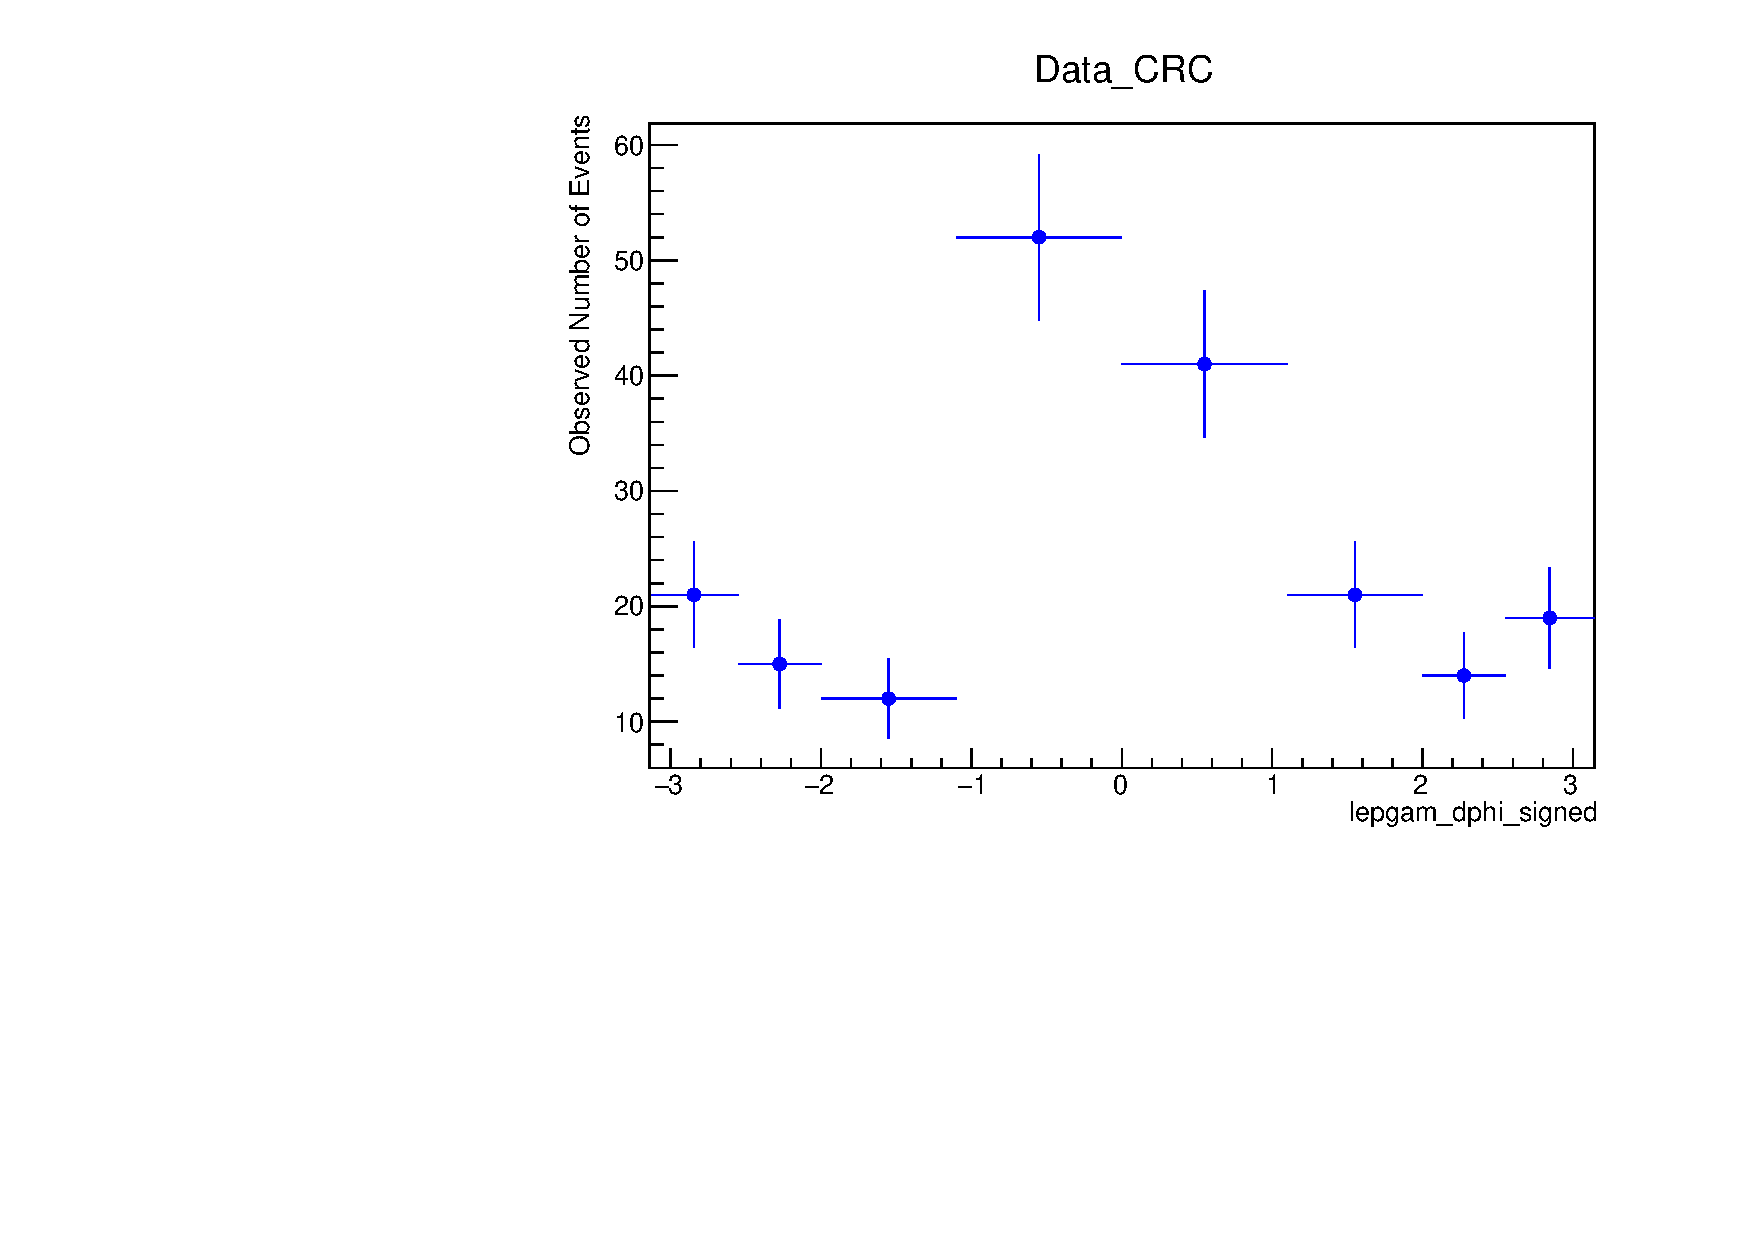
\includegraphics[width=0.48\textwidth]{plots/diffx/Data_CRC_lepgam_dphi_signed.pdf}
  }
  \caption{The observed numbers of events for \dphisigned and \lepgamdphi in the CRs. These distributions are consistent with being symmetric. \label{fig:data_dphi}}
\end{figure}

The symmetrisation is performed by taking the weighted arithmetic mean of paired bins given by

\begin{equation}
  x_{ij}=\frac{w_ix_i+w_jx_j}{w_i+w_j},
\end{equation}

where $x_{ij}$ is the averaged value of the observable $x$ in paired bins $i$ and $j$, and the weights $w_i$ are given by $w_i=\frac{1}{\epsilon_i^2}$, where $\epsilon_i$ is the error in bin $i$.

%\clearpage
\section{Testing of the Binned Likelihood Fit}

A number of tests of the likelihood fit were performed using the Asimov dataset to ensure that it performed as expected. The most basic test is that perfect closure is achieved when fitting the nominal Asimov dataset constructed using the \SHERPA \qcdwy sample against the nominal MC templates, which are also defined using the \SHERPA \qcdwy sample. Perfect closure is observed for all observables. 

As another test of the fit, the QCD template was halved in the low \Ngapjets regions to test that the residual correction, $c$, would yield exactly $c=2$. The QCD template was also halved simultaneously in the SR and CRa to test that \bl would yield a value of 2, and in CRb and CRc to test that \bh would yield a value of 2. In this test, the fit parameters were seen to correspond exactly to the expected values. 

As a third test of the signal extraction, an Asimov dataset is constructed using the alternate \MADGRAPH \qcdwy MC sample (rather than the nominal \SHERPA sample). Figure \ref{fig:vbswy:mgasimovprefit} shows the \mjj prefit yields for this configuration. From this it is clear that the \MADGRAPH \qcdwy prediction is higher than the \SHERPA prediction in the SR for all bins. In CRa, the agreement is relatively good in all bins. The \MADGRAPH prediction undershoot in bins 2 and 4 in CRb, and overshoots in all but the last bin in CRc. The modelling of the dominant background is therefore very dependent on the kinematic region, which highlights the importance of deriving bin depending corrections in addition to a residual correction factor.  

The likelihood fit is then performed with this configuration, and the postfit results of the fit parameters \muew, \bl, \bh, and $c$, are compared with expectations derived from logical arguments. This test is performed for all observables, however, only \mjj is shown here for brevity. Figure \ref{fig:vbswy:mgasimovpostfit} shows the postfit yields, and Figure \ref{fig:vbswy:mgasimovpars} shows the constrained values of the parameters after the fit. The postfit agreement is good in the SR and CRa, where the statistical precision of the data and fit templates is superior, and conversely, the agreement is slightly worse in CRb and CRc.

\begin{figure}[t]
  \centering
  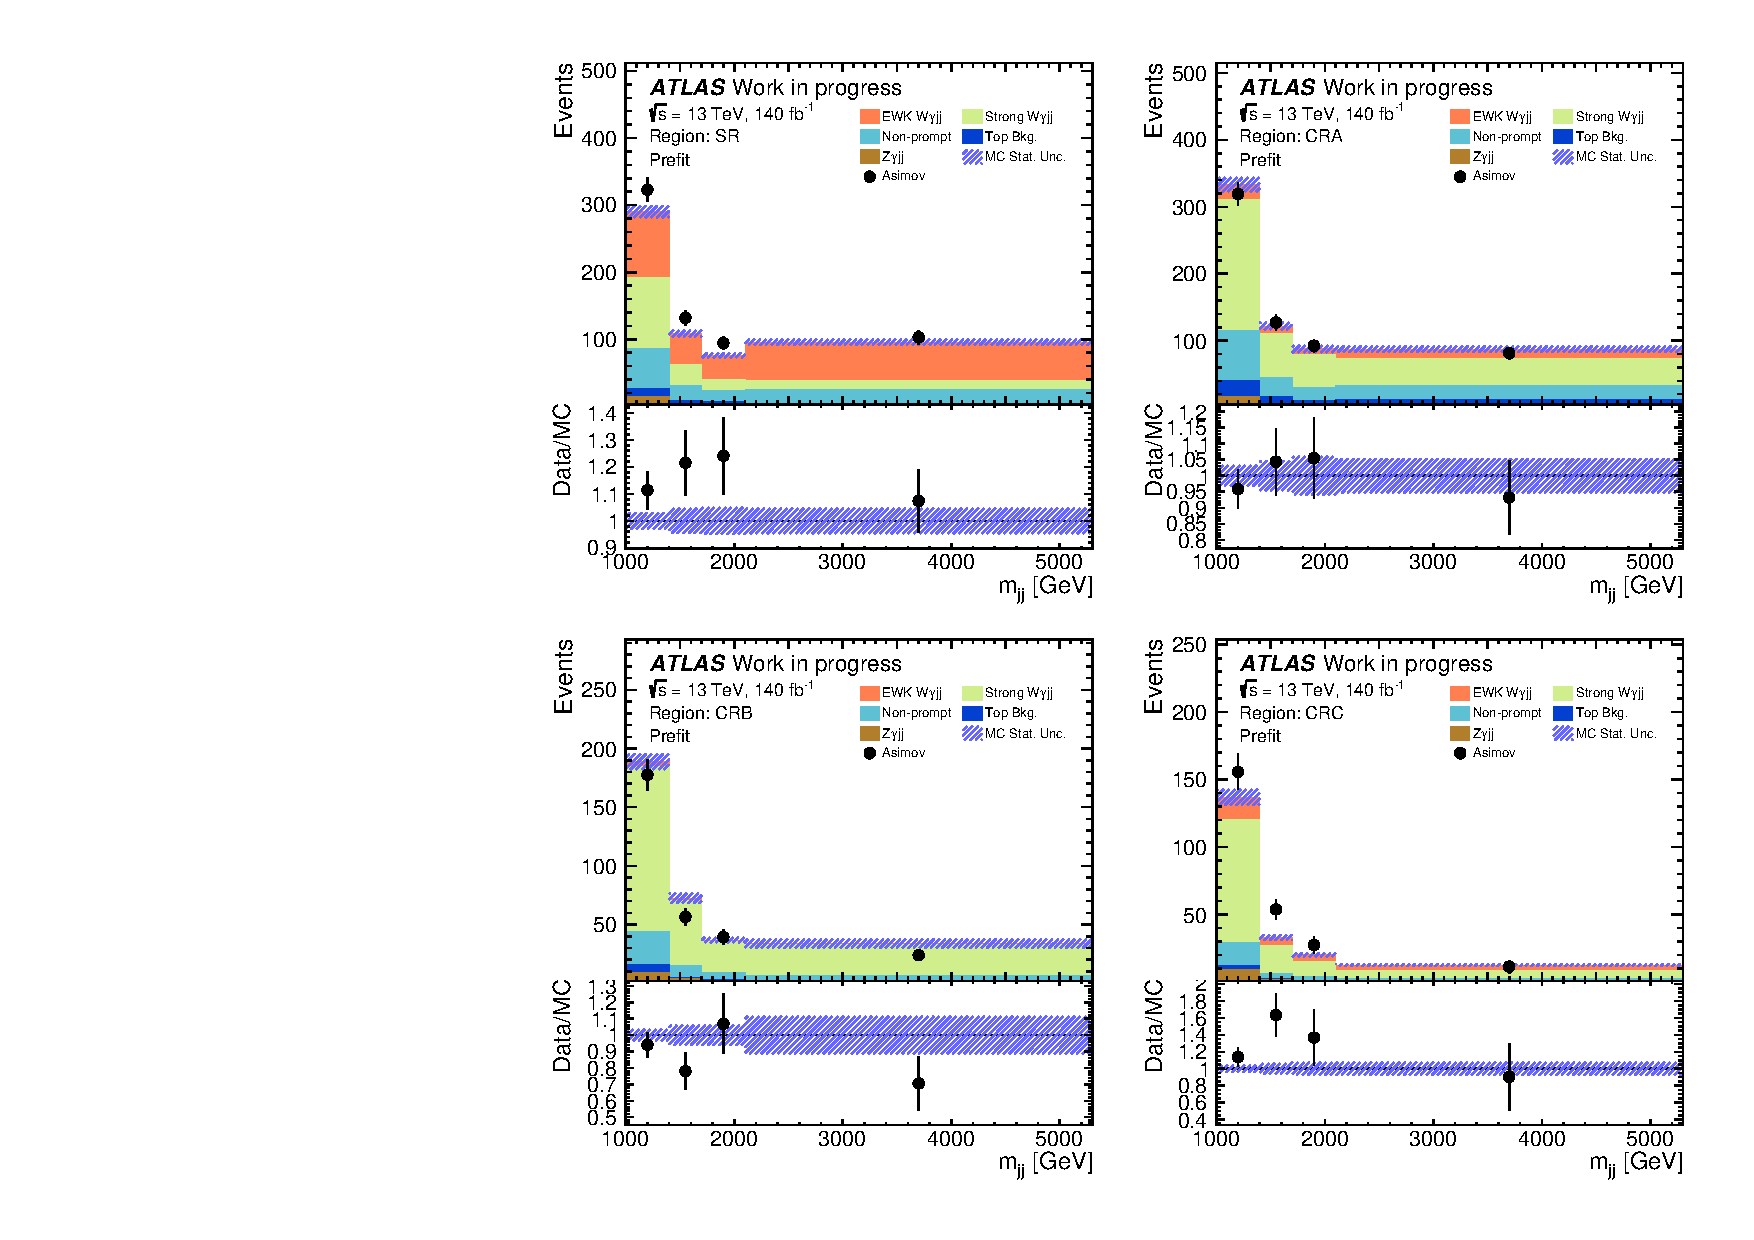
\includegraphics[width=\textwidth]{plots/diffx/mgasimovtest/mjj_prefit_data_30Nov.pdf}
  \caption{Prefit differential event yields with the Asimov dataset constructed using the \MADGRAPH \qcdwy sample.\label{fig:vbswy:mgasimovprefit}}
\end{figure}

Since \bl is applied in CRa, this parameter is primarily constrained in CRa. Therefore, the expectation from Figure \ref{fig:vbswy:mgasimovprefit} is that \bl takes values (<1,>1,>1,<1). Similarly, \bh is applied in CRb and CRc, but the \qcdwy background in CRc is constrained by an additional parameter, $c$. Therefore, \bh is primarily constrained in CRb. From Figure \ref{fig:vbswy:mgasimovprefit}, \bh should take the values (<1,<1,>1,<1). Finally, since $c$ is applied in CRc, $c$ is constrained primarily by CRc. Furthermore, \bh should have an average correction of about 0.85 (taking the average of the Asimov/MC values in CRb), which after applying to CRc results in an Asimov/MC disagreement in CRc of about 1.5 on average. Therefore $c$ is expected to be about 1.5. \muew is then determined in the SR after applying \bl and $c$ to the \qcdwy background. The postfit fit parameters shown in Figure \ref{fig:vbswy:mgasimovpars} broadly confirm the expectation of this simple consideration.

\begin{figure}[t]
\centering
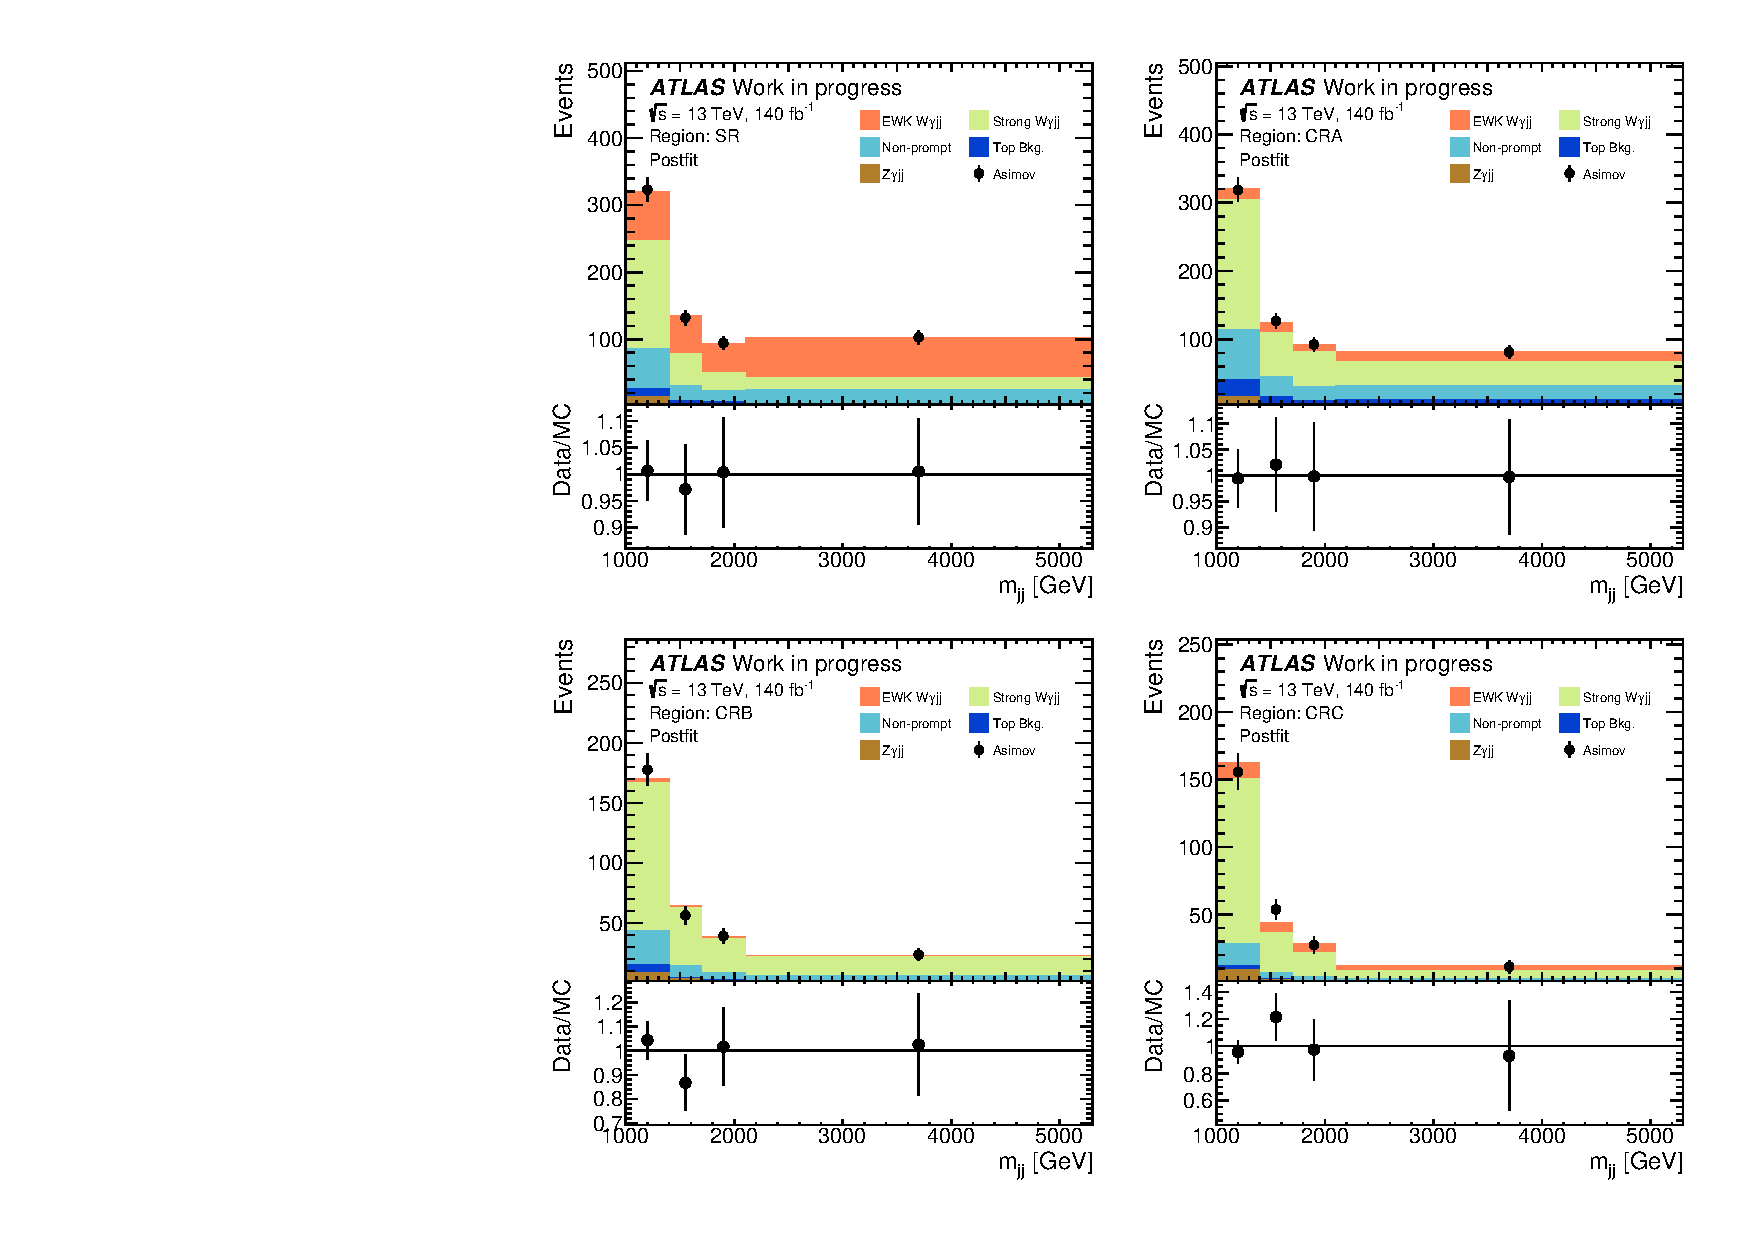
\includegraphics[width=\textwidth]{plots/diffx/mgasimovtest/mjj_postfit_data_30Nov.pdf}
\caption{Postfit event yields for the fit with the Asimov dataset constructed from the \MADGRAPH \qcdwy sample.\label{fig:vbswy:mgasimovpostfit}}
\end{figure}

\begin{figure}[t]
\begin{subfigure}[b]{0.48\textwidth}
    \centering
    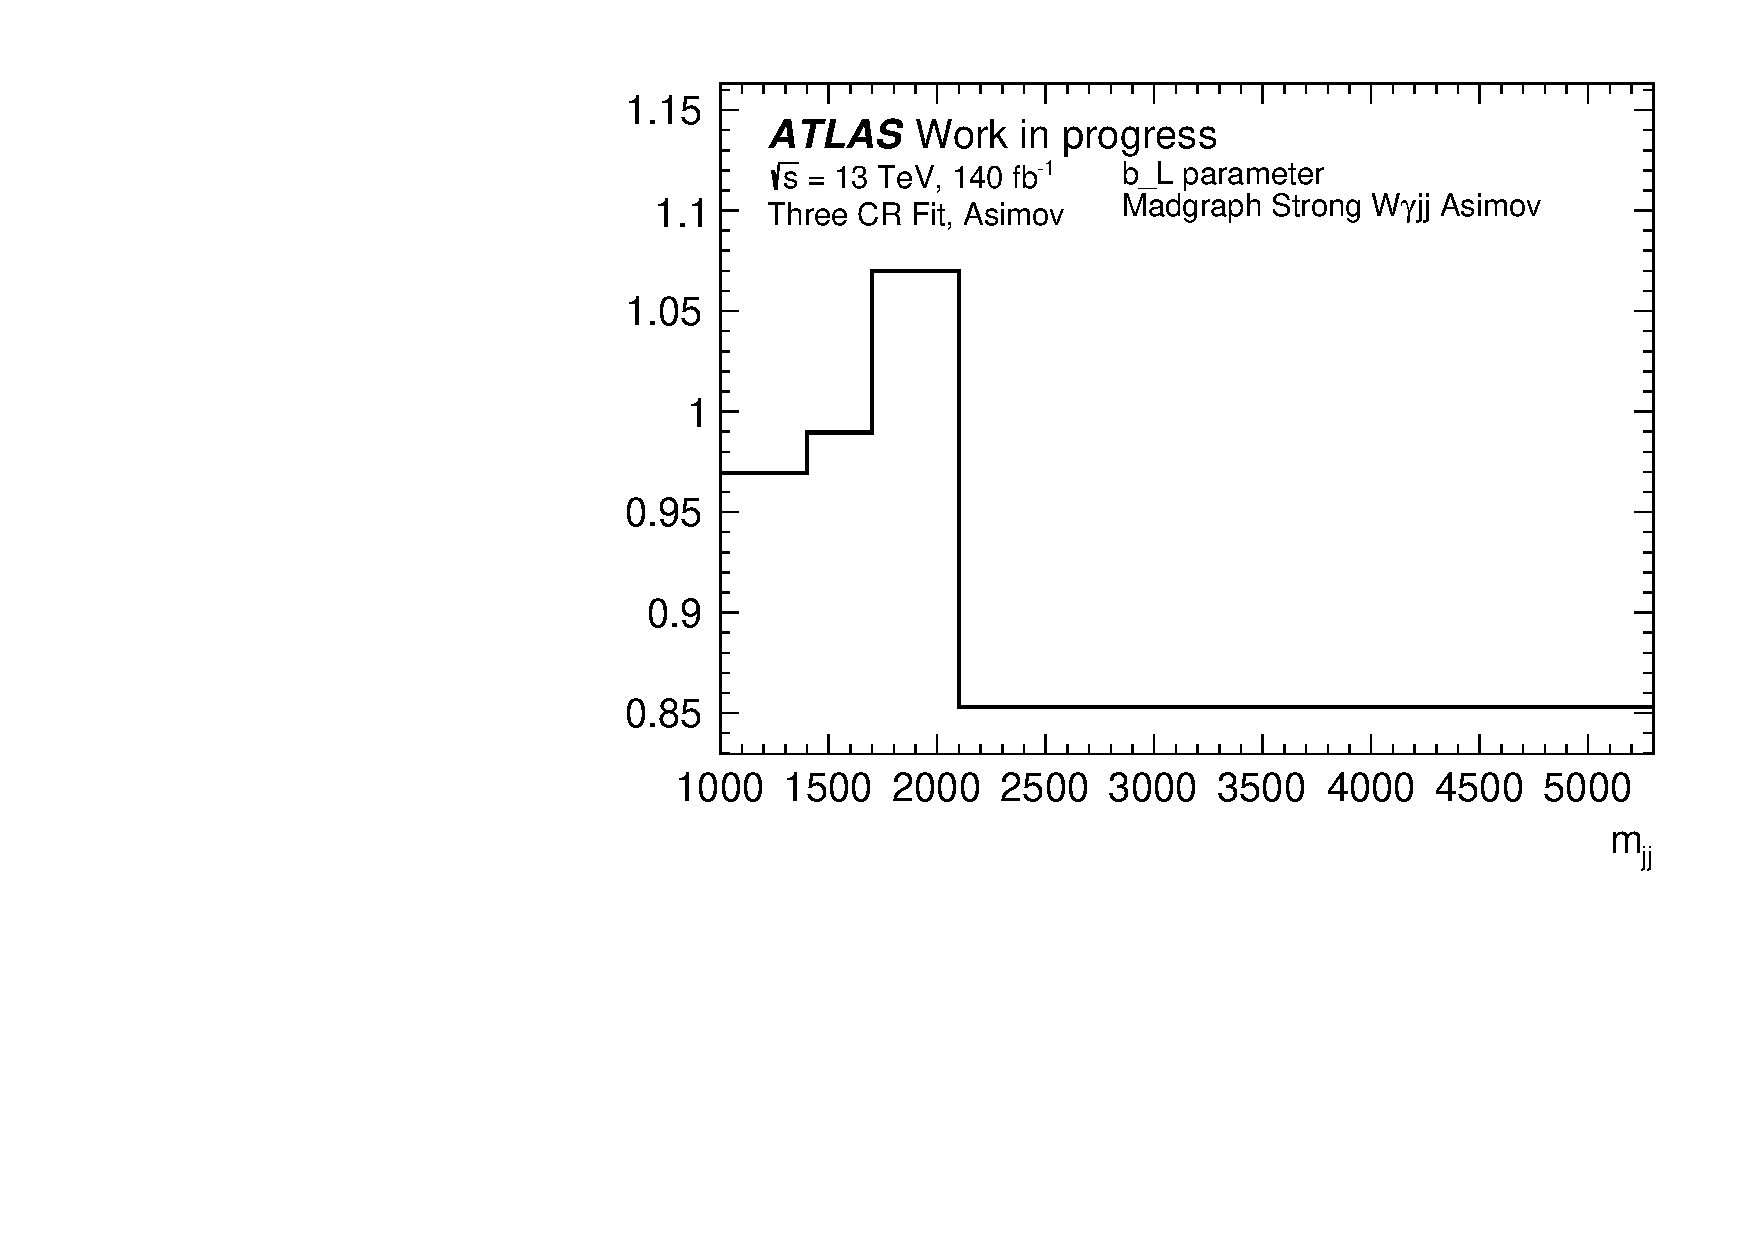
\includegraphics[width=\textwidth]{plots/diffx/mgasimovtest/b_LWyC_constant_fx_mjj.pdf}
    \caption{}
\end{subfigure}
\hfill
\begin{subfigure}[b]{0.48\textwidth}
    \centering
    \includegraphics[width=\textwidth]{plots/diffx/mgasimovtest/b_HWyC_constant_fx_mjj.pdf}
    \caption{}
\end{subfigure}
\begin{subfigure}[b]{0.48\textwidth}
    \centering
    \includegraphics[width=\textwidth]{plots/diffx/mgasimovtest/c_constant_fx_mjj.pdf}
    \caption{}
\end{subfigure}
\hfill
\begin{subfigure}[b]{0.48\textwidth}
    \centering
    \includegraphics[width=\textwidth]{plots/diffx/mgasimovtest/muEW_constant_fx_mjj.pdf}
    \caption{}
\end{subfigure}
\caption{The constrained fit parameters for the fit with the Asimov dataset constructed from the \MADGRAPH \qcdwy sample. (a) corresponds to the parameter \bl, (b) to \bh, (c) to $c$, and (d) to \muew. These are seen to be consistent with expectations from logical arguments. The fact that \muew does not equal 1 is a reflection of the uncertainty on the extracted \ewwy yield due to the choice of MC generator in the \qcdwy sample.\label{fig:vbswy:mgasimovpars}}
\end{figure}

The values of the constrained fit parameters align well with the expectations described above. The only deviation from the expectation is in the second bin for the \bl parameter, where the value is just below 1, whereas the expectation was that this would be greater than 1. This is explained by the fact that there is some signal leakage into the control regions, and background leakage into the signal region. Therefore the assumptions made above do not hold perfectly. 

%\clearpage
\section{Choice of Function for the Residual Correction}\label{sec:vbswy:fxchoice}

In equation \ref{eq:strongmcfit2} the choice is made for the residual correction to take the form of a constant factor $c$. However, without this factor, there are \nbins degrees of freedom remaining. Therefore, this residual correction factor can in principle take the form of a polynomial, or any other function with up to \nbins free parameters. For the discussion in this chapter, the residual correction function is denoted by \fx, where $i$ runs over the number of bins of the observable $x$. The following choices of function are investigated:
\begin{itemize}
  \item $\fx=1$,
  \item $\fx=c$,
  \item $\fx=mx_i+c$.
\end{itemize}

\subsection{\fx=1}

With \fx=1, the signal extraction method is equivalent to a fit with one control region, i.e. there is no residual correction applied. It can seen from Figure \ref{fig:vbswy:mgasimovprefit} that this would not adequately constrain the dominant background. With this configuration the only \qcdwy constraint is derived in CRa, and the difference between the \qcdwy \SHERPA and \MADGRAPH predictions in this region are only of the order of $5-10\%$. Therefore the data-to-MC disagreement in the SR is resolved primarily through shifts in \muew. It is clear that there are large modelling differences between the low and high centrality regions which are not captured by a single constraint to the \qcdwy background. A residual correction factor is therefore absolutely necessary to prevent the measurement from being limited by background modelling uncertainties. This configuration also results in larger systematic uncertainties, which can can be seen in Section \ref{sec:vbswy:extraction_uncertainties}.

\subsection{$\fx=mx_i+c$ or $\fx=c$}\label{sec:vbswy:fitinstab}

It is possible that the data-to-MC non-closure is not uniform after applying the \bl constraint in the SR. In fact, this was seen in \cite{VBSWy:VBFZ}. Allowing \fx to depend on an extra parameter, means the signal extraction is sensitive to this non-uniformity. However, the addition of an extra parameter results in the procedure being less robust to statistical fluctuations. This is true particularly of \mjj, where all but the first bin in CRc have fewer than 30 expected events. This puts into question whether probing the shape of the non-closure is valid, and if it will lead to robust results. To test this, the signal is extracted for 1000 pseudo-experiments, where for each pseudo-experiment the \qcdwy fit template in a given region is fluctuated in accordance with the statistical uncertainties\footnote{This is done by multiplying each event weight by a list of 1000 random numbers sampled from a Poisson distribution of unit mean.}. For each fluctuation, the extracted signal is recorded, and the result is plotted on a 2D histogram of \qcdwy template fluctuation vs post-fit \ewwy yield. This is repeated for each region, separately. The goal of this test is to understand how a given statistical fluctuation is able to affect the extracted \ewwy yield. If the likelihood fit is robust, then small statistical fluctuations in the templates should lead to small changes in the extracted \ewwy yield. The results of this test are shown in Figure \ref{fig:lastbin_mjj_instabilities} for the fourth bin of \mjj, where the \MADGRAPH \qcdwy template is used, and the \MADGRAPH \qcdwy sample is used in the construction of the Asimov dataset\footnote{For this test, the Asimov dataset is constructed using the \MADGRAPH \qcdwy template because this particular configuration does a good job at highlighting the unstable behaviour of the fit. The fit ought to be stable regardless of how the Asimov dataset is defined, hence any undesirable behaviour observed for this configuration should be treated with equal importance as the nominal configuration (where the Sherpa-2.2.11 \qcdwy template is used to construct the Asimov dataset).}.

\begin{figure}[t]
  \centering
  \includegraphics[width=\textwidth]{plots/diffx/instab/linearfx/instabilities_mjj_QCD_Mgraph_Signal_Sh2211_BSMCQCDSTATS_linearfx_newbinning_madgraphasimov_bin4.pdf}
  \caption{The relative shift in the extracted electroweak yield in bin-4 of \mjj for the linear $f(x)$ definition when fitting using the \MADGRAPH \qcdwy template, and \MADGRAPH \qcdwy Asimov definition. The $x$-axis is the shift in the \qcdwy template from the nominal, and the $y$-axis is the shift in the extracted EW yield. Particularly in CRc, small fluctuations in the QCD template result in very large fluctuations in the extracted EW yield result. \label{fig:lastbin_mjj_instabilities}}
\end{figure}

The CRc subfigure in Figure \ref{fig:lastbin_mjj_instabilities} shows that the likelihood fit is not robust when $\fx=mx_i+c$ is used. Shifts of $<20\%$ in the \qcdwy template result in $50-100\%$ shifts in the extracted \ewwy yield. Moreover, there are only around 5 MC events in this bin in CRc which lead to the $50-100\%$ shifts in the extracted yield. Therefore, because \fx is allowed too much freedom to float, the statistical precision of \muew is compromised by a small prediction for the background. If the likelihood fit is robust, a small background prediction should lead to a more precise prediction on \muew, and not the other way round. 

Figure \ref{fig:fxconstantinstab} shows the same thing as Figure \ref{fig:lastbin_mjj_instabilities}, except now \fx is defined to be a constant factor, i.e. $\fx=c$. With this configuration, a $20\%$ shift in the \qcdwy template in CRc leads to a shift in \muew of about $10-20\%$. Removing a degree of freedom in the definition of \fx has resolved the problems seen in Figure \ref{fig:lastbin_mjj_instabilities}. With $\fx=c$, the high-occupancy first bin of \mjj now primarily constrains this factor, and the final result is much more robust to statistical fluctuations. To summarise, restricting the residual correction to a constant factor leads to significantly more robust predictions of \muew. 

\begin{figure}[t]
  \centering
  \includegraphics[width=\textwidth]{plots/diffx/instab/constfx/instabilities_mjj_QCD_Mgraph_Signal_Sh2211_BSMCQCDSTATS_madgraphasimov_bin4.pdf}
  \caption{Relative yield results in the fourth bin of \mjj for the $\fx=c$ fit. From the CRc plot it can be seen that the poor QCD statistics here no longer have an impact on the stability of the fit. Additionally, the statistical precision on the extracted yield due to fluctuations in CRc has improved by a factor of 4 by switching to $\fx=c$ from $\fx=mx_i+c$. \label{fig:fxconstantinstab}}
\end{figure}

The 2D plots shown above were constructed for all possible configurations, and for all bins of all observables to check the robustness of the likelihood fit. The different configurations explore the effects of fluctuating the Asimov dataset, rather than the \qcdwy template; and using the \SHERPA sample or the \MADGRAPH sample in either constructing the \qcdwy template or the Asimov dataset. With $\fx=mx_i+c$, many similar plots to Figure \ref{fig:lastbin_mjj_instabilities} with unstable behaviour are observed. In contrast, all of the 2D plots for the $\fx=c$ definition are consistent with robust fit behaviour. These plots are shown in Appendix \ref{sec:appendix:stability} for other bins of \mjj (the other observables are omitted for brevity). 

It is also worth commenting on the shapes of the 2D distributions in Figures \ref{fig:lastbin_mjj_instabilities} and \ref{fig:fxconstantinstab}. For $\fx=c$, The shapes are roughly ellipsoidal in nature, suggesting that $\mu_{EW}$ is roughly Gaussian distributed. This is not the case for the $\fx=mx_i+c$ definition. The Gaussian shape is potentially more desirable as a more symmetrical distribution of pseudo-experiments corresponds to a smaller statistical bias, which makes the results easier to interpret. The results are not completely free of bias, and this is clear in the upward turning shape in CRa. This happens because there is an inherent asymmetry associated with fluctuating the \qcdwy template statistics, in that the purity of the signal increases with shifts to lower values, and decreases with shifts to higher values of the \qcdwy yield.

The choice of $\fx=c$ is made for this analysis since it resolves the robustness issues mentioned for $\fx=mx_i+c$. Appendix \ref{sec:appendix:stability:fxc} shows the $\fx=c$ stability plots for \mjj. All results shown outside of this Section and Appendix \ref{sec:appendix:stability:fxlinear} are for the $\fx=c$ definition. It is worth noting that with this definition, there will be a relatively large range of integrated yields between observables. This is because it is likely that \fx does in fact have a non-uniform shape, which results in the overall normalisation of the \qcdwy background being constrained to variable values depending on the observable. To resolve this issue, the option of adding an additional Gaussian constraint to the likelihood was explored. This term would then act to constrain the overall normalisation of the \qcdwy background such that there are only very small fluctuations between observables. In adding this term, the final systematic uncertainties were seen to be biased significantly. Therefore, no such constraint is added in the final signal extraction method. Moreover, the integrated yields are seen to be statistically consistent between observables, therefore there are no actual inconsistencies between the results of different observables. 

\clearpage
\section{Uncertainties}\label{sec:vbswy:extraction_uncertainties}

The uncertainties on the extracted \ewwy yield are split into systematic and statistical uncertainties. The systematic uncertainties are divided into theoretical uncertainties, which affect the shape and normalisation of the MC samples, and experimental uncertainties, which affect the event reconstruction. The systematic uncertainties are broken down into components that are fully correlated between bins and regions. This means that, for every systematic variation, the templates are varied simultaneously in the signal and control regions before constructing the likelihood.

A complete list of experimental uncertainties is given in Section \ref{sec:expsysts_extraction}, the dominant experimental uncertainties are Jet Energy Scale (JES) and Jet Energy Resolution (JER) uncertainties. The theoretical uncertainties on the measurement are described in Section \ref{sec:vbswy:theoryunc}. The dominant theoretical uncertainty is from \qcdwy generator choice. 
%
%USE THIS TEXT FOR THE THEORY UNC SECTION: the PDF and QCD scale uncertainties for the \qcdwy, \ewwy, and prompt backgrounds; $\alpha_s$ uncertainties for the \qcdwy, \ewwy, and QCD-Z$\gamma$ backgrounds (only for the \SHERPA samples); renormalization and factorization scale uncertainties on the EW and QCD-$W\gamma$ background as well as the prompt background, generator choice uncertainties for the \qcdwy and \ewwy backgrounds, lumi, interference %The combinations of factorisation and renormalization scale parameters used as systematic variations are described in Section \ref{sec:theory_systs_scale}.
%In this section, the effect that these uncertainties have on the extracted EW signal is described.

\subsection{Data Statistical Uncertainties}\label{sec:stat_unc_extraction}

To determine the statistical uncertainty on the extracted \ewwy yield due to the statistical precision of the data (referred to as data stat uncertainty), 10,000 pseudo-experiments are created from the data sample, where for each pseudo-experiment, the bin contents are sampled from a Poisson distribution of mean equal to the original bin yields. In generating the pseudo-experiments, each region and bin is sampled independently using different a different random number seed. The extracted \ewwy yield is recorded for each of the 10,000 pseudo-experiments. The RMS of the extracted \ewwy yields of the pseudo-experiments is taken as the data statistical uncertainty. Figures \ref{fig:stats_data_toys_1} and \ref{fig:stats_data_toys_2} show the pseudo-experiments for each of the observables for two example bins in \mjj and \leppt, respectively. In each case they are consistent with a Gaussian distribution. For the first bin on \mjj, there is small spike at zero caused by the large width of the Gaussian in this bin. The width is large in the first bin because there is a large background contamination at low \mjj which results in larger uncertainties in the extracted \ewwy yield. In the case of \leppt, the background contamination is not so large in the first bin which results in a more narrow Gaussian, and therefore there is no spike around 0.%Figure \ref{fig:stats_data_toys_1} for the distributions of extracted \ewwy yields for \mjj, \ptjj, and \dphisigned. Figure \ref{fig:stats_data_toys_2} shows the \leppt, \lepgamdphi, and \lym distributions. 

\begin{figure}[t]
  \centering
  \includegraphics[width=0.49\textwidth]{plots/diffx/statunc/data/Gaussians/sys_bin_errors_mjj_gaus_bin1_Data_Statistics.pdf}
  %\includegraphics[width=0.24\textwidth]{plots/diffx/statunc/data/Gaussians/sys_bin_errors_mjj_gaus_bin2_Data_Statistics.pdf}
  \includegraphics[width=0.49\textwidth]{plots/diffx/statunc/data/Gaussians/sys_bin_errors_mjj_gaus_bin3_Data_Statistics.pdf}
  %\includegraphics[width=0.24\textwidth]{plots/diffx/statunc/data/Gaussians/sys_bin_errors_mjj_gaus_bin4_Data_Statistics.pdf}
  %\includegraphics[width=0.24\textwidth]{plots/diffx/statunc/data/Gaussians/sys_bin_errors_jj_pt_gaus_bin1_Data_Statistics.pdf}
  %\includegraphics[width=0.24\textwidth]{plots/diffx/statunc/data/Gaussians/sys_bin_errors_jj_pt_gaus_bin2_Data_Statistics.pdf}
  %\includegraphics[width=0.24\textwidth]{plots/diffx/statunc/data/Gaussians/sys_bin_errors_jj_pt_gaus_bin3_Data_Statistics.pdf}
  %\includegraphics[width=0.24\textwidth]{plots/diffx/statunc/data/Gaussians/sys_bin_errors_jj_pt_gaus_bin4_Data_Statistics.pdf}
  %\includegraphics[width=0.24\textwidth]{plots/diffx/statunc/data/Gaussians/sys_bin_errors_jj_pt_gaus_bin5_Data_Statistics.pdf}
  %\includegraphics[width=0.24\textwidth]{plots/diffx/statunc/data/Gaussians/sys_bin_errors_jj_dphi_gaus_bin1_Data_Statistics.pdf}
  %\includegraphics[width=0.24\textwidth]{plots/diffx/statunc/data/Gaussians/sys_bin_errors_jj_dphi_gaus_bin2_Data_Statistics.pdf}
  %\includegraphics[width=0.24\textwidth]{plots/diffx/statunc/data/Gaussians/sys_bin_errors_jj_dphi_gaus_bin3_Data_Statistics.pdf}
  %\includegraphics[width=0.24\textwidth]{plots/diffx/statunc/data/Gaussians/sys_bin_errors_jj_dphi_gaus_bin4_Data_Statistics.pdf}
  %\includegraphics[width=0.24\textwidth]{plots/diffx/statunc/data/Gaussians/sys_bin_errors_jj_dphi_gaus_bin5_Data_Statistics.pdf}
  %\includegraphics[width=0.24\textwidth]{plots/diffx/statunc/data/Gaussians/sys_bin_errors_jj_dphi_gaus_bin6_Data_Statistics.pdf}
  \caption{The pseudo-experiment extracted yields for \mjj for the first and third bins. Each pseudo-experiment represents represents a statistical fluctuation in the data. The RMS' of these distributions form the data stat uncertainty, $R^{\text{stat}}$. Note that the mean values in each of these plots do not correspond exactly to the central value of the extracted yield (the prescription is to average over all data and MC pseudo-experiments, rather than only pseudo-experiments in data). For display purposes, the shapes of the pseudo-experiments are fit with a Gaussian omitting the bin at zero.}\label{fig:stats_data_toys_1}
\end{figure}

\begin{figure}[t]
  \centering
  \includegraphics[width=0.49\textwidth]{plots/diffx/statunc/data/Gaussians/sys_bin_errors_lep_pt_gaus_bin1_Data_Statistics.pdf}
  %\includegraphics[width=0.24\textwidth]{plots/diffx/statunc/data/Gaussians/sys_bin_errors_lep_pt_gaus_bin2_Data_Statistics.pdf}
  %\includegraphics[width=0.24\textwidth]{plots/diffx/statunc/data/Gaussians/sys_bin_errors_lep_pt_gaus_bin3_Data_Statistics.pdf}
  \includegraphics[width=0.49\textwidth]{plots/diffx/statunc/data/Gaussians/sys_bin_errors_lep_pt_gaus_bin4_Data_Statistics.pdf}
  %\includegraphics[width=0.24\textwidth]{plots/diffx/statunc/data/Gaussians/sys_bin_errors_lep_pt_gaus_bin5_Data_Statistics.pdf}
  %\includegraphics[width=0.24\textwidth]{plots/diffx/statunc/data/Gaussians/sys_bin_errors_lepgam_dphi_gaus_bin1_Data_Statistics.pdf}
  %\includegraphics[width=0.24\textwidth]{plots/diffx/statunc/data/Gaussians/sys_bin_errors_lepgam_dphi_gaus_bin2_Data_Statistics.pdf}
  %\includegraphics[width=0.24\textwidth]{plots/diffx/statunc/data/Gaussians/sys_bin_errors_lepgam_dphi_gaus_bin3_Data_Statistics.pdf}
  %\includegraphics[width=0.24\textwidth]{plots/diffx/statunc/data/Gaussians/sys_bin_errors_lepgam_dphi_gaus_bin4_Data_Statistics.pdf}
  %\includegraphics[width=0.24\textwidth]{plots/diffx/statunc/data/Gaussians/sys_bin_errors_lepgam_dphi_gaus_bin5_Data_Statistics.pdf}
  %\includegraphics[width=0.24\textwidth]{plots/diffx/statunc/data/Gaussians/sys_bin_errors_lepgam_dphi_gaus_bin6_Data_Statistics.pdf}
  %\includegraphics[width=0.24\textwidth]{plots/diffx/statunc/data/Gaussians/sys_bin_errors_lepgam_dphi_gaus_bin7_Data_Statistics.pdf}
  %\includegraphics[width=0.24\textwidth]{plots/diffx/statunc/data/Gaussians/sys_bin_errors_lepgam_dphi_gaus_bin8_Data_Statistics.pdf}
  %\includegraphics[width=0.24\textwidth]{plots/diffx/statunc/data/Gaussians/sys_bin_errors_ly_m_gaus_bin1_Data_Statistics.pdf}
  %\includegraphics[width=0.24\textwidth]{plots/diffx/statunc/data/Gaussians/sys_bin_errors_ly_m_gaus_bin2_Data_Statistics.pdf}
  %\includegraphics[width=0.24\textwidth]{plots/diffx/statunc/data/Gaussians/sys_bin_errors_ly_m_gaus_bin3_Data_Statistics.pdf}
  %\includegraphics[width=0.24\textwidth]{plots/diffx/statunc/data/Gaussians/sys_bin_errors_ly_m_gaus_bin4_Data_Statistics.pdf}
  %\includegraphics[width=0.24\textwidth]{plots/diffx/statunc/data/Gaussians/sys_bin_errors_ly_m_gaus_bin5_Data_Statistics.pdf}
  \caption{The extracted yields of the pseudo-experiments for \leppt for the first and fourth bins. Each pseudo-experiment represents represents a statistical fluctuation in the data.}\label{fig:stats_data_toys_2}
\end{figure}

%From Figure \ref{fig:stats_data_toys} it can be seen that for \mjj and \ptjj, there is a spike at zero caused by Gaussian tail of the distribution reaching the boundary of 0 numbers of events. For \dphisigned this is less prominant. Hence there is a slight bias with \mjj and \ptjj which results in the mean of the toys being smaller than the integrated yield of the input Signal template in the SR. This discrepancy is at a level greater than $1/\sqrt(10000)=1\%$, hence this cannot be attributed to a lack toy distributions. Additionally, the overflow bins are designed to hold fewer than 1 event for each observable, hence this doesn't account for the discrepancy either. 

%The integrated extracted EW yields, and data statistical uncertainties for \mjj, \ptjj and \dphisigned are 231.9$\pm 39.6$ , 232.1$\pm 34.3$, 236.9$\pm 27.8$ respectively, whereas the input signal template has an integrated yield in the SR of 236.90. Note that it is difficult for the total absolute statistical uncertainties to be directly compared between observables because the statistical resolution of the extracted yield in a given bin is dependent on every other bin due to the correlations induced between bins by $f(x)$. Additionally, the statistical precision of the \dphisigned extracted yield is expected to be better than the other observables due to the fact that the bin-dependent factors $b_L$ are shared between symmetric bins. 

%\begin{equation}\label{eq:rms_data}
%  R^{\text{stat}}=\frac{\text{RMS}_{\text{Data}}(N_{\text{EW, Sherpa},i})}{\langle N_{\text{EW, Sherpa},i}\rangle_{\text{Data}}}
%\end{equation}

\subsection{MC Statistical Uncertainties}\label{sec:vbswy:mcstats}
The statistical uncertainty on the extracted \ewwy yield due to the combined statistical precision of the MC samples (referred to as MC stat uncertainty) is evaluated similarly to the data stat uncertainty, by creating 10,000 pseudo-templates in the signal region and the control regions, and propagating each combination of pseudo-experiments through the likelihood fit. The only difference with the MC stat uncertainty calculation is in the preparation of the pseudo-experiments. Instead of sampling from a Poisson distribution of mean equal to the bin content, each MC weight is multiplied by an integer sampled from a unit Poisson distribution. The reason for the difference in the pseudo-experiment preparation methods is that when it comes to keeping track of correlations between nominal and systematic MC templates, the latter approach must be used. This is explained in more detail in Section \ref{sec:expsysts_extraction}.  %\textit{bootstraps} of all the MC templates in the SR and in all CRs. A bootstrap is a replica fluctuated according to a unit Poisson distribution in such a way as to keep track of correlations - see Section \ref{sec:expsysts_extraction} for a more complete description of bootstrapping (keeping track of the correlations is not relevant for evaluating the MC stat uncertainties).
%The signal extraction is performed separately for each bootstrap. After extracting the signal, the relative MC stat uncertainty is given by
%The MC stat uncertainty is given by
%\begin{equation}
%  R^{\text{syst}}_{\text{MC Stats}}=\text{RMS}_{\text{MC}}(N_{\text{EW, Sherpa},i}).
%\end{equation}

The relative data and MC stat uncertainties are shown in Figure \ref{fig:vbswy:statsdata} for the signal extraction in data. The relative statistical uncertainties are calculated with respect to the nominal extracted yield given by 
\begin{equation}\label{eq:central_value_extraction}
  N_{\text{EW}}^{\text{Nom}} \equiv \langle N_{\text{EW},i}\rangle,
\end{equation}
where $N_{\text{EW},i}$ is the postfit \ewwy yield in the signal region, and the index $i$ runs over 10,000 pseudo-experiment, where for each pseudo-experiment, the data and all MC templates are fluctuated in all CRs and the SR before performing the signal extraction. The angled brackets denote taking the mean value. The reason for taking the mean of the pseudo-experiments is because there is a slight bias in the toy distributions which results in the mean lying away from the nominal value. Not doing this would result in asymmetric uncertainties. %is to avoid issues with systematics for example generator modelling, which can potentially result in the nominal value lying far away from the mean of the pseudo-experiments.
%
%\begin{figure}[t]
%  \centering
%  \includegraphics[width=0.48\textwidth]{plots/diffx/statunc/asimov/relative_datastats_mjj_27Nov.pdf}
%  \includegraphics[width=0.48\textwidth]{plots/diffx/statunc/asimov/relative_datastats_jj_pt_27Nov.pdf}
%  \includegraphics[width=0.48\textwidth]{plots/diffx/statunc/asimov/relative_datastats_jj_dphi_27Nov.pdf}
%  \includegraphics[width=0.48\textwidth]{plots/diffx/statunc/asimov/relative_datastats_ly_m_27Nov.pdf}
%  \includegraphics[width=0.48\textwidth]{plots/diffx/statunc/asimov/relative_datastats_lep_pt_27Nov.pdf}
%  \includegraphics[width=0.48\textwidth]{plots/diffx/statunc/asimov/relative_datastats_lepgam_dphi_27Nov.pdf}
%  \caption{Statistical uncertainty on the central value $N_{\text{EW,Nominal}}$ for \mjj, \ptjj, \dphisigned, \mly, \leppt, \lepgamdphi, where the Asimov dataset is used. Note that the slight asymmetry of the \lepgamdphi and \dphisigned is because the random seeds chosen for any given pair of bins are not the same when deriving the pseudo-experiments. The red line indicates the data stat uncertainty and the green line indicates MC stat uncertainty on the extracted \ewwy yield.}
%  \label{fig:vbswy:statsasimov}
%\end{figure}

\begin{figure}[t]
  \centering
  \includegraphics[width=0.48\textwidth]{plots/diffx/statunc/data/relative_datastats_mjj_27Nov.pdf}
  \includegraphics[width=0.48\textwidth]{plots/diffx/statunc/data/relative_datastats_jj_pt_27Nov.pdf}
  \includegraphics[width=0.48\textwidth]{plots/diffx/statunc/data/relative_datastats_jj_dphi_27Nov.pdf}
  \includegraphics[width=0.48\textwidth]{plots/diffx/statunc/data/relative_datastats_ly_m_27Nov.pdf}
  \includegraphics[width=0.48\textwidth]{plots/diffx/statunc/data/relative_datastats_lep_pt_27Nov.pdf}
  \includegraphics[width=0.48\textwidth]{plots/diffx/statunc/data/relative_datastats_lepgam_dphi_27Nov.pdf}
  %\caption{Statistical uncertainty on the central value $N_{\text{EW,Nominal}}$ for \mjj, \ptjj, \dphisigned, \mly, \leppt, \lepgamdphi. Note that the data stat uncertainties on the \lepgamdphi and \dphisigned observables are not exactly the same using Asimov data. This is because the random seeds chosen for any given pair of bins are not the same when deriving the Asimov toys. The red line indicates $R^{\text{stat}}$ and the green line indicates $R^{\text{syst}}_{\text{MC Stats}}$. textcolor{red}{FIX THIS CAPTION}}
  \caption{Statistical uncertainty on the central value $N_{\text{EW,Nominal}}$ for \mjj, \ptjj, \dphisigned, \mly, \leppt, \lepgamdphi, where data is used.}
  \label{fig:vbswy:statsdata}
\end{figure}

\subsection{Treatment of Systematic Uncertainties}

Before going on to describe the different sources of systematic uncertainties, it is useful to outline the processing of the systematic uncertainties.

\subsubsection{Bootstrapping and statistical significance}

In order to understand how systematic uncertainties are treated in this analysis, it is necessary to introduce the \textit{bootstrapping} procedure. This procedure allows for the statistical uncertainty on each systematic uncertainty to be determined. Consider one set of MC events where, for example, the Jet Energy Scale (JES) is fixed at its nominal value and the same set of events where the JES is fixed at a slightly different value. The events remain entirely correlated, one just has a different scaling for the jet energies and \pt. One of the implications of this correlation is that in order to determine the statistical uncertainty on the JES (from taking the difference in extracted yields derived the using nominal and varied templates), the standard error propagation formalism cannot be used, since this assumes uncorrelated uncertainties. One way to approach this problem is through the \textit{bootstrapping} procedure, where $N_{\text{bootstraps}}$ pseudo-experiments are constructed for the nominal case and for each systematic variation. These bootstraps are created by multiplying each MC event weight by a random number sampled from a unit (discrete) Poisson distribution. The bootstraps are created in such a way as to preserve the correlations between the nominal pseudo-experiment numbered $i$, and systematic one corresponding to the same number. The correlations are preserved by choosing the random number for a given event when creating the nominal and systematic MC templates. 1000 pseudo-experiments is determined to be sufficient for calculating the statistical uncertainty in the systematic uncertainties.%Since the MC and data stat uncertainties are the largest uncertainties on the measurement, it is impotartant that a sufficient number of bootstraps is used to determine these precisely. 

Note that the random number seeds for the bootstrapping procedure are chosen according to the run number and event number. The statistical uncertainties are calculated by constructing each pseudo-experiment and constructing a new likelihood. 

The statistical uncertainty of each systematic is important because this provides information about the statistical significance of the systematic uncertainty, i.e. how likely it is that the difference between the nominal and systematic extracted yields is not due to statistical fluctuations. To decide whether an uncertainty is statistically insignificant, the significance threshold, $\sigma_{\text{thresh}}$, is defined, where if the systematic uncertainty is greater than $\sigma_{\text{thresh}}$ times its statistical uncertainty, it is deemed to be statistically significant. In this analysis, a systematic uncertainty is deemed to be statistically significant if the significance in at least one of the observable bins is greater than $\sigma_{\text{thresh}}$. If the systematic uncertainty is statistically insignificant, it is set to zero in all bins. Three values of $\sigma_{\text{thresh}}$ and their corresponding impact to the systematic uncertainties were investigated. These are $\sigma_{\text{thresh}} = 1.6, \sigma_{\text{thresh}} = 1.0$, and $\sigma_{\text{thresh}} = 0$. In the end, it was decided to quote the systematic uncertainties at the level of $\sigma_{\text{thresh}} = 0$, i.e. to keep all systematic uncertainties since the difference in overall systematic uncertainty on the extracted yield is very small between the choices by virtue of the fact that the most statistically insignificant systematic uncertainties are also those which have the smallest impact. See Appendix \ref{sec:appendix:sigthresholds} for the final uncertainties on the extracted yield with each choice of significance threshold. %See Appendix \ref{app:sig_extra_sigthreshold} for a discussion of this.

\subsubsection{Smoothing procedure}

All systematic uncertainties except for the uncertainties from the non-prompt background estimates are smoothed. Those which have their statistical significance evaluated using bootstrapping are smoothed through a Linear Gaussian Kernel smoothing algorithm \cite{VBSWy:kernelsmooth}, which uses the statistical errors on the systematic uncertainties as inputs to the smoothing algorithm. Using Gaussian Kernel smoothing reduces the likelihood of over-smoothing, i.e. where the smoothed value is far away from what would expected from statistical fluctuations.%In this algorithm, the smoothing is applied in such a way as to ensure the smoothed values are statistically insignificant, i.e. the smoothing is consistent with the statistical fluctuations of the systematic uncertainties. The algorithm works by first dividing the x-axis range into 100 separate points. A straight line is fit through all permutations of pairs of coordinates corresponding to the histogram bin values, and each straight line is then evaluated at $x$. The evaluated value is $y_i$, and the error on $y_i$, $\epsilon_i$, is calculated by propagating the histogram bin errors. For each $y_i$, a weight is assigned according to the product of $1/\epsilon_i^2$ and two Gaussian kernels of variable width centred at each x-axis value of the coordinate pair. The weighted average of all the $y_i$ is the final smoothed value at $x$. The algorithm starts with a Gaussian kernel width of 0.5, and this is gradually increased until the smoothed values are statistically significant at a level of at most $1\sigma$, where the statistical significance is determined using a chi-squared test. The smoothed graph (consisting of 100 coordinate values) is then evaluated at the original histogram bin centers to give the final smoothed histogram. 

The theory uncertainties on the $Z\gamma$ and top backgrounds do not have their statistical significance evaluated using bootstrapping. This is because these uncertainties are very small, and deriving the bootstrapping is computationally expensive. These uncertainties are smoothed using the Root TH1::Smooth(3) function. This completes three iterations of the ``353QH, twice'' algorithm outlined in the 1974 Cern School of Computing proceedings \cite{VBSWy:thsmoothing}. This is a running median smoothing algorithm that uses a combination of operations given by its name, where the integers refer to the window size, ``Q'' refers to quadratic interpolation, ``H'' refers to the use the Hann function, and ``twice'' refers to doubling the sequence.

The smoothing is always performed on the relative uncertainties. The smoothed relative uncertainties are applied to $N_{\text{EW}}^{\text{Nom}}$ to get the final absolute uncertainties.

\subsubsection{Symmetrising}

 All experimental uncertainties, and some data-driven background uncertainties have ``up'' and ``down'' variations, where for example the JES is increased (up) and decreased (down) with respect to the nominal JES. These variations are propagated separately through the likelihood before symmetrising, and the sign of the shift is kept during the symmetrisation. The symmetrised uncertainties are unfolded using the response matrices corresponding to the ``up'' variation.

\subsection{Experimental Systematic Uncertainties}\label{sec:expsysts_extraction}

The following experimental uncertainties are included:

\begin{itemize}
  \item Jet uncertainties \cite{Atlas:smallrcali}:
  \begin{itemize}
  \item The \verb+EffectiveNP+ JES nuisance parameters which capture the uncertainties from the in-situ calibrations ($\gamma/Z$+jet and multi-jet balance). 
  \item Other JES uncertainties coming from the eta-intercalibration, pileup, flavour-related, and punch-through uncertainty sources. 
  \item The \verb+EffectiveNP+ JER nuisance parameters which capture uncertainties from the noise term and di-jet in-situ sources.  
  \item Differences between the MC and data in the JER.
  \item Flavour tagging uncertainties
  \item Precision flavour uncertainties
  \item Vertex tagging
  \item $b-$tagging uncertainties
  \end{itemize} 
  \item Electron and muon uncertainties including uncertainties \cite{Atlas:egam_reco_gsf,Atlas:egam_reco,Atlas:muonreco}:
  \begin{itemize}
    \item Identification efficiency scale factors
    \item Isolation efficiency scale factors 
    \item Reconstruction efficiency scale factors
    \item Trigger efficiency scale factors
    \item Energy scale and resolution
    \item Track-to-vertex-association (TTVA) -- muons only
    % \item Bad muon veto efficiency -- muons only
  \end{itemize}
  \item Photon uncertainties including uncertainties from \cite{Atlas:egam_reco_gsf,Atlas:egam_reco}:
  \begin{itemize}
    \item Photon energy resolution
    \item Photon energy scale
  \end{itemize}
  \item \met uncertainties including uncertainties \cite{Atlas:met}:
  \begin{itemize}
    \item Soft track resolution
    \item Soft track scale
  \end{itemize}
  \item Pileup reweighting (PRW) uncertainties\footnote{PRW refers to the correction of the pileup profile in simulation to that of data using a set of weights.}
  \item Uncertainty in the integrated luminosity (\pm0.83\%) \cite{LHC:atlaslumi}
\end{itemize}

The dominant sources of experimental uncertainties come from JER and JES sources. This is because VBS events are primarily characterised by kinematic parameters relating to jets (see the VBS cuts in table \ref{tab:vbswy:analysiscuts}). Therefore scale and resolution effects relating to jets can have a large impact on the number of selected events in the analysis phasespace.

The signal is extracted using the nominal templates for 1000 bootstraps, and separately using the templates corresponding to the experimental systematic nuisance parameters. For any given nuisance parameter (e.g. ``JER\textunderscore EffectiveNP\textunderscore\textunderscore 1up''), the \qcdwy, \ewwy and prompt background yields are all varied simultaneously according to this nuisance parameter -- i.e. the experimental uncertainties are treated as correlated between samples. The nominal systematic uncertainty for a given systematic variation is calculated by determining the average deviation from the nominal for each bootstrap, divided by the average of all the nominal bootstraps. The relative experimental uncertainty on the central value for the extracted EW yield is denoted as $R^{\text{sys}}_{\text{exp}}$

\begin{equation}\label{eq:expunc}
  R^{\text{sys}}_{\text{exp}} = \frac{\langle N_{\text{EW},i}^{\text{Nom}}-N_{\text{EW}, i}^{\text{exp}}\rangle}{\langle N_{\text{EW},i}^{\text{Nom}}\rangle},\hspace{5pt} \Delta R^{\text{sys}}_{\text{exp}} = \frac{\text{RMS}(N_{\text{EW},i}^{\text{Nom}}-N_{\text{EW}, i}^{\text{exp}})}{\langle N_{\text{EW},i}^{\text{Nom}}\rangle},
\end{equation}
where the extracted EW yield in the SR, for bootstrap $i$, corresponding to a systematic variation is denoted $N_{\text{EW}, i}^{\text{exp}}$. And the extracted EW yield for bootstrap $i$, corresponding to the nominal is denoted as $N_{\text{EW},i}^{\text{Nom}}$.

The statistical uncertainties on $R^{\text{sys}}_{\text{exp}}$, denoted here as $\Delta R^{\text{sys}}_{\text{exp}}$ are evaluated by subtracting each systematic bootstrap from the nominal bootstrap, and taking the RMS of the resulting distributions.\footnote{There is small technicality in the calculation of the relative uncertainties prior to smoothing, in that the pseudo-experiments in the denominator are always the same pseudo-experiments as those in the numerator. Therefore $\langle N_{\text{EW},i}^{\text{Nom}}\rangle$ is not exactly the same as the nominal yield $N_{\text{EW}}^{\text{Nom}}$ in equation \ref{eq:central_value_extraction}, since this is calculated from MC+data stat pseudo-experiments. It's also worth pointing out that when there is no bootstrapping performed, the value in the denominator for the relative uncertainty calculation is always the nominal yield without any average over pseudo-experiments.} 
Figure \ref{fig:expuncexamples} shows an example selection of individual systematic uncertainties (before symmetrising up and down variations) and the smoothing of these uncertainties using their statistical errors. The results of smoothing and symmetrising the up and down variations for a selection of jet uncertainty sources and a selection of other experimental sources are shown for \mjj in Figures \ref{fig:vbswy:jesvariationsmjj} and \ref{fig:vbswy:otherexpvariationsmjj}, respectively. These show the individual variations in the central value due to experimental uncertainty sources for the extracted EW yield and the relative uncertainties. 

\begin{figure}[t]
  \includegraphics[width=0.48\textwidth]{plots/diffx/expsysts/indiv/sys_errors_jj_dphi_QCD_Sh2211_Signal_Sh2211_BSEXPSYSTS_PRW_DATASF__1up_3cr.pdf}
  \includegraphics[width=0.48\textwidth]{plots/diffx/expsysts/indiv/sys_errors_mjj_QCD_Sh2211_Signal_Sh2211_BSEXPSYSTS_JET_JER_EffectiveNP_7__1up_3cr.pdf}
  \caption{Examples of smoothed experimental systematic uncertainties in \dphisigned and \mjj. Error bars on the relative systematic uncertainties are statistical uncertainties derived using bootstrapping. The statistical uncertainties are used in the smoothing algorithms, the results of which are shown by the blue and red lines. The red line is used as the final systematic uncertainty for all bootstrapped systematic uncertainties.}
  \label{fig:expuncexamples}
\end{figure}

\begin{figure}[t]
  %\includegraphics[width=0.48\textwidth]{plots/diffx/expsysts/groups/mjj_QCD_Sh2211_BSEXPSYSTS_3cr_JET_EffectiveNP_0p01sigma_allvariations.pdf}
  \includegraphics[width=0.48\textwidth]{plots/diffx/expsysts/groups/mjj_QCD_Sh2211_BSEXPSYSTS_3cr_JET_EtaIntercalibration_0p01sigma_allvariations.pdf}
  \includegraphics[width=0.48\textwidth]{plots/diffx/expsysts/groups/mjj_QCD_Sh2211_BSEXPSYSTS_3cr_JET_Pileup_0p01sigma_allvariations.pdf}
  \includegraphics[width=0.48\textwidth]{plots/diffx/expsysts/groups/mjj_QCD_Sh2211_BSEXPSYSTS_3cr_JET_Other_0p01sigma_allvariations.pdf}
  \includegraphics[width=0.48\textwidth]{plots/diffx/expsysts/groups/mjj_QCD_Sh2211_BSEXPSYSTS_3cr_JER_0p01sigma_allvariations.pdf}
  \caption{Example of relative uncertainties due to the different JES and JER variations propagated to the final extracted EW yield with \mjj.}
  \label{fig:vbswy:jesvariationsmjj}
\end{figure}

\begin{figure}[t]
\begin{subfigure}[b]{0.48\textwidth}
    \centering
    \includegraphics[width=\textwidth]{plots/diffx/expsysts/groups/mjj_QCD_Sh2211_BSEXPSYSTS_3cr_MET_0p01sigma_allvariations.pdf}
    \caption{}
\end{subfigure}
\begin{subfigure}[b]{0.48\textwidth}
    \centering
    \includegraphics[width=\textwidth]{plots/diffx/expsysts/groups/mjj_QCD_Sh2211_BSEXPSYSTS_3cr_PRW_0p01sigma_allvariations.pdf}
    \caption{}
\end{subfigure}
\caption{Relative uncertainties due to \met (a) and PRW (b) systematic variations variations propagated to the final extracted EW yield with \mjj.}
\label{fig:vbswy:otherexpvariationsmjj}
\end{figure}

\subsection{Non-prompt Background Uncertainties}

The uncertainties on the non-prompt background estimates as described in Section \ref{sec:vbswy:nonprompt} are propagated to the extracted EW yield by simply shifting the data-driven background template in the fit corresponding to the uncertainty, where this is correlated between regions. Statistical uncertainties on the templates are treated in the same was as MC stat uncertainties in the likelihood -- i.e. they are included in the construction of the Poisson constraints. Additionally, statistical uncertainties are explicitly included as up and down variations when shifting the templates. There is no bootstrapping performed for uncertainties on the data-driven backgrounds, and there is also no smoothing performed on the final uncertainties on the extracted EW yield. The reason for not smoothing is because, without bootstrapping to determine their statistical significance, these uncertainties could easily be oversmoothed. 

The uncertainties on the extracted \ewwy yield from the non-prompt backgrounds are shown for the \mjj distribution in Figure \ref{fig:vbswy:fakesvariations}. The other observables are omitted for brevity.

\begin{figure}[t]
  \centering
  \includegraphics[width=\textwidth]{plots/diffx/expsysts/groups/mjj_QCD_Sh2211_FAKES_3cr_FAKE_0p01sigma_allvariations.pdf}
  \caption{}
  \caption{Relative uncertainties on the extracted \ewwy yield from the non-prompt background estimates with \mjj.}
  \label{fig:vbswy:fakesvariations}
\end{figure}

\subsection{Theoretical Uncertainties}\label{sec:vbswy:theoryunc}

Theoretical uncertainties affect the shape and normalisation of the individual MC backgrounds. These effects are not correlated between the backgrounds, therefore theoretical uncertainties are calculated for each background separately and are all added in quadrature in the calculation of the total theoretical uncertainty on the extracted \ewwy yield.

The theoretical uncertainties considered are (i) scale uncertainties, which characterise missing high order corrections in perturbative QCD calculations; (ii) uncertainties in the strong coupling constant $\alpha_\mathrm{s}$; (iii) PDF uncertainties; (iv) generator choice uncertainties; and (v) the effect of the interference between the \qcdwy and \ewwy processes.
 
\subsubsection{\Qcdwy Generator Choice}\label{sec:genchoiceextraction}

There is a significant difference in the modelling of the \qcdwy background between the \SHERPA and \MADGRAPH MC generators. In order probe the degree to which the measurement depends on the of background model, it an uncertainty is assigned to this choice. 

The \qcdwy generator choice uncertainty before smoothing, $R^{\text{sys}}_{\text{gen}}$, is calculated by extracting an EW yield in the SR for both \qcdwy templates for 10,000 bootstraps over the \qcdwy templates. The difference in extracted yield is computed for every pair of bootstraps, and the mean over all bootstraps is taken. This is turned into a relative uncertainty by dividing by the central value; i.e. 

\begin{equation}\label{eq:genchoicetheory}
  R^{\text{sys}}_{\text{gen}} = \frac{\langle N_{\text{EW},i}^{\text{Nom, Sherpa}}-N_{\text{EW},i}^{\text{Nom, MG5}}\rangle}{\langle N_{\text{EW},i}^{\text{Nom, Sherpa}}\rangle}, \hspace{5pt} \Delta R^{\text{sys}}_{\text{gen}} = \frac{\text{RMS}(N_{\text{EW},i}^{\text{Nom, Sherpa}}-N_{\text{EW},i}^{\text{Nom, MG5}})}{\langle N_{\text{EW},i}^{\text{Nom, Sherpa}}\rangle},
\end{equation}

where the index $i$ runs over bootstraps (note that even though the index $i$ is the same for \SHERPA and \MADGRAPH, these bootstraps are uncorrelated). The statistical uncertainty on $R^{\text{sys}}_{\text{gen}}$ is denoted by $\Delta R^{\text{sys}}_{\text{gen}}$, and is evaluated by taking the standard deviation (denoted RMS) for each pair of bootstraps. The \qcdwy generator choice uncertainties are shown in Figure \ref{fig:vbswy:genchoicedata}. 

\begin{figure}[t]
  \centering
  \includegraphics[width=0.49\textwidth]{plots/diffx/genchoice/data/sys_errors_mjj_generator_choice_3cr.pdf}
  \includegraphics[width=0.49\textwidth]{plots/diffx/genchoice/data/sys_errors_jj_pt_generator_choice_3cr.pdf}
  \includegraphics[width=0.49\textwidth]{plots/diffx/genchoice/data/sys_errors_jj_dphi_generator_choice_3cr.pdf}
  \includegraphics[width=0.49\textwidth]{plots/diffx/genchoice/data/sys_errors_ly_m_generator_choice_3cr.pdf}
  \includegraphics[width=0.49\textwidth]{plots/diffx/genchoice/data/sys_errors_lep_pt_generator_choice_3cr.pdf}
  \includegraphics[width=0.49\textwidth]{plots/diffx/genchoice/data/sys_errors_lepgam_dphi_generator_choice_3cr.pdf}
  \caption{Data QCD generator choice uncertainties with \mjj, \ptjj, \dphisigned, \mly, \leppt, and \lepgamdphi before and after smoothing. Note that because $\fx=c$ introduces correlations between the bins, the statistical error bars are correlated between bins.}
  \label{fig:vbswy:genchoicedata}
\end{figure}

The statistical uncertainty of the generator choice uncertainties is relatively high, this is evident in the around 20-30\% statistical uncertainties on the $R_{\text{gen}}^{\text{sys}}$ values. The reason for this is that, since the \SHERPA and \MADGRAPH predictions are statistically independent, the statistical uncertainties on the generator choice is the quadrature sum of the individual statistical uncertainties. Furthermore, the statistical precision of the \MADGRAPH sample is around 2.3 times worse than the \SHERPA sample, hence the statistical resolution of the combined uncertainty is limited by the precision of the \MADGRAPH sample.\footnote{Ideally, a new \MADGRAPH sample would have been generated with a similar statistical precision to the nominal \SHERPA sample. However, this was not done because of time limitations, and because these samples already contain over 100 million events each.} The fact that it is difficult to statistically resolve these uncertainties is one of the main motivating factors behind choosing the Gaussian kernel smoothing algorithm over the root TH1 smoothing. It is evident from the last bin of the \leppt plot in Figure \ref{fig:vbswy:genchoicedata}, that choosing the TH1 smoothing would have resulted in an over-smoothed uncertainty -- i.e. the smoothed value is $>2\sigma$ above the nominal value in the last bin. It is important to note that this choice -- as with any analysis optimisation decision -- was made based on blinded Asimov results.%These Asimov results are shown in Figure \ref{fig:vbswy:genchoiceasimov}.
%In Figure xyz, none of the bins are separated by $>1\sigma$, which could imply that the statistical uncertainties are overestimated. However, these statistical uncertainties should really be represented as asymmetric uncertainties. This is because as the \qcdwy yield fluctuates downward, the leakage into the signal region decreases. Similarly, as the \qcdwy yield fluctuates upward, the leakage into the signal region increases.  With a greater degree of leakage, \muew has more freedom to float, resulting in large uncertainties on the extracted \ewwy yield. Similarly, with less leakage, \muew has less freedom to float. This effect can be seen in Figure xyz, which shows the results of fluctuating the \MADGRAPH \qcdwy sample on the \ewwy yield in second bin of \jjdphi. Due to time constraints, these uncertainties are represented in the symmetric way shown.
%\begin{figure}[H]
%  \centering
%  \includegraphics[width=0.6\textwidth]{plots/diffx/genchoice_toys_bins_jjdphi.pdf}
%  \caption{Test}
%\end{figure}

The generator choice uncertainties are consistent with zero. This is somewhat expected as the three control region fit is designed to be robust against modelling uncertainties due to the additional residual correction, $\fx=c$. Without this residual correction, the generator choice uncertainties are significantly larger, as shown in Figure \ref{fig:vbswy:genchoicedataonecr} where $\fx=1$. Even though $R_{\text{gen}}^{\text{sys}}$ is consistent with zero, the conservative approach is taken to still include these uncertainties after smoothing.

\begin{figure}[t]
  \centering
  \includegraphics[width=0.49\textwidth]{plots/diffx/genchoice/data/sys_errors_mjj_generator_choice_1cr.pdf}
  \includegraphics[width=0.49\textwidth]{plots/diffx/genchoice/data/sys_errors_jj_pt_generator_choice_1cr.pdf}
  \includegraphics[width=0.49\textwidth]{plots/diffx/genchoice/data/sys_errors_jj_dphi_generator_choice_1cr.pdf}
  \includegraphics[width=0.49\textwidth]{plots/diffx/genchoice/data/sys_errors_ly_m_generator_choice_1cr.pdf}
  \includegraphics[width=0.49\textwidth]{plots/diffx/genchoice/data/sys_errors_lep_pt_generator_choice_1cr.pdf}
  \includegraphics[width=0.49\textwidth]{plots/diffx/genchoice/data/sys_errors_lepgam_dphi_generator_choice_1cr.pdf}
  \caption{Data QCD generator choice uncertainties for the $\fx=1$ (equivalently one control region) configuration with \mjj, \ptjj, \dphisigned, \mly, \leppt, and \lepgamdphi before and after smoothing. It is clear that the generator choice uncertainty on the measurement is no longer consistent with zero, but fluctuates around 30-40\% instead.}
  \label{fig:vbswy:genchoicedataonecr}
\end{figure}


\subsubsection{\ewwy Generator Choice}

The uncertainty due to the choice of MC generator in the \ewwy sample is evaluated in almost the same way as the \qcdwy generator choice, where now the \MADGRAPH \ewwy sample is used as the alternate sample. The only difference is that the \ewwy generator choice uncertainties are not smoothed. The reason for not smoothing these uncertainties is that in order to evaluate the final uncertainty after unfolding, the extracted yield using \MADGRAPH has be to unfolded using the response matrix from the same sample. This is called the ``hidden variables test'', and aims to probe the effect of MC shape differences in the unfolding procedure which are not covered by detector simulation uncertainties. Therefore, the smoothing is not implemented in order to prevent smoothing over valid effects from hidden variables. The data \ewwy generator choice uncertainty results is shown for \mjj in Figure \ref{fig:vbswy:genchoiceewdata}, where the other observables are omitted for brevity. The uncertainty is below 5\% in all bins of \mjj, and therefore represents a relatively unimportant contribution. The differences between the \SHERPA and \MADGRAPH \ewwy simulations are primarily in the overall normalisation, therefore the choice of generator in the simulation of the signal corresponds to only a small uncertainty on the extracted \ewwy yield.

\begin{figure}[t]
  \centering
  \includegraphics[width=0.75\textwidth]{plots/diffx/genchoice/data/sys_errors_mjj_generator_choice_ew_3cr.pdf}
  \caption{Data EW generator choice uncertainties with \mjj before and after smoothing. The smoothing has a small effect on the final uncertainty.\label{fig:vbswy:genchoiceewdata}}
\end{figure}

\subsubsection{Scale Uncertainties}

The theoretical calculation of the $pp$ collision cross-section for a particular process depends on \muf, \mur, and \alphas. These symbols denote the factorisation scale, renormalisation scale, and the strong coupling constant. The factorisation scale represents the momentum scale at which particles couple to each other. The renormalisation scale describes the running of the strong coupling constant, \alphas. The factorisation and renormalisation scale are associated with collinear and ultraviolet divergences in higher-order contributions to the hard scatter, respectively, and can be chosen independently in the perturbative calculation of the collision cross-section. Since the hard scatter depends on \muf and \mur, varying these scales is a way of estimating contributions from missing higher orders \cite{VBSWy:Behnke}. 

For each sample, the (\muf,\mur) combination is altered by multiplicative factors of (1.0, 1.0), (1.5, 1.0), (1.0, 1.5), (0.5, 1.0), (1.0, 1.5), (2.0, 1.0), and (1.0, 2.0) to evaluate these uncertainties. For every (\muf,\mur) combination the \ewwy yield is extracted, and the systematic uncertainty is calculated from:

\begin{equation}\label{eq:scaleunc}
  R^{\text{sys}}_{(\mu_F,\mu_R)} = \frac{\langle N_{\text{EW},i}^{\text{Nom}}-N_{\text{EW}, i}^{(\mu_F,\mu_R)}\rangle}{\langle N_{\text{EW},i}^{\text{Nom}}\rangle},
\end{equation}

where $R^{\text{sys}}_{(\mu_F,\mu_R)}$ is the uncertainty from a given (\muf, \mur) combination, $N_{\text{EW}, i}^{(\mu_F,\mu_R)}$ is the corresponding extracted \ewwy yield, and $i$ represents the bootstrap pseudo-experiments. No average over bootstraps is taken for the $Z\gamma$jj and top scale uncertainties as no bootstrapping is performed for these samples. The final uncertainty due to scale variations is given by the envelope of all the $R^{\text{sys}}_{(\mu_F,\mu_R)}$ values, where the envelope is defined by:

\begin{equation}\label{eq:scaleunc}
  R^{\text{sys}}_{\text{scale}} = \text{max}_{(\muf,\mur)}(R^{\text{sys}}_{(\mu_F,\mu_R)}),
\end{equation}

where the maximum is taken over the different (\muf,\mur) values. For the calculation of the unfolded uncertainties, the individual variations corresponding to $R^{\text{sys}}_{(\mu_F,\mu_R)}$ are unfolded prior to taking the envelope.

The scale uncertainties for data are shown for the \mjj distribution in \ref{fig:vbswy:scaledata}, where the other observables are omitted for brevity. Changes in the renormalisation and factorisation scale primarily result is shifts in the normalisation, where these can be as high as 45\% in the \SHERPA \qcdwy sample. However, because the likelihood fit is robust to changes in normalisation, these get constrained in the fit and only result in a small systematic effect on the extracted \ewwy yield. The largest uncertainty comes from scale variations the $Z\gamma$jj sample. This is because the normalisation of this template is not constrained in the fit. However, these uncertainties are below $4\%$, and so are still considered small.

\begin{figure}[t]
  \begin{subfigure}[b]{0.49\textwidth}
    \centering
    \includegraphics[width=\textwidth]{plots/diffx/scalesysts/data/mjj_QCD_Sh2211_BSSTRONGTHEORYSYSTS_3cr_Scale_0p01sigma_allvariations.pdf}
    \caption{}
  \end{subfigure}
  \hfill
  \begin{subfigure}[b]{0.49\textwidth}
    \centering
    \includegraphics[width=\textwidth]{plots/diffx/scalesysts/data/mjj_QCD_Sh2211_BSEWTHEORYSYSTS_3cr_Scale_0p01sigma_allvariations.pdf}
    \caption{}
  \end{subfigure}
  \hfill
  \begin{subfigure}[b]{0.49\textwidth}
    \centering
    \includegraphics[width=\textwidth]{plots/diffx/scalesysts/data/mjj_QCD_Sh2211_QCDZGAMMATHEORYSYSTS_3cr_Scale_0p01sigma_allvariations.pdf}
    \caption{}
  \end{subfigure}
  \hfill
  \begin{subfigure}[b]{0.49\textwidth}
    \centering
    \includegraphics[width=\textwidth]{plots/diffx/scalesysts/data/mjj_QCD_Sh2211_EWKZGAMMASHERPATHEORYSYSTS_3cr_Scale_0p01sigma_allvariations.pdf}
    \caption{}
  \end{subfigure}
  \hfill
  \begin{subfigure}[b]{0.49\textwidth}
    \centering
    \includegraphics[width=\textwidth]{plots/diffx/scalesysts/data/mjj_QCD_Sh2211_TQGAMMATHEORYSYSTS_3cr_Scale_0p01sigma_allvariations.pdf}
    \caption{}
  \end{subfigure}
  \hfill
  \begin{subfigure}[b]{0.49\textwidth}
    \centering
    \includegraphics[width=\textwidth]{plots/diffx/scalesysts/data/mjj_QCD_Sh2211_TTGAMMATHEORYSYSTS_3cr_Scale_0p01sigma_allvariations.pdf}
    \caption{}
  \end{subfigure}
  \caption{Scale uncertainties on the \qcdwy background (a), \ewwy signal (b), strong $Z\gamma$jj background (c), EW strong $Z\gamma$jj background (d), non-negligible top backgrounds (e,f) propagated to the extracted \ewwy yield with \mjj. \label{fig:vbswy:scaledata}}
\end{figure}

\subsubsection{\alphas uncertainties}

The theoretical MC precictions depend on Standard Model parameters such as the strong coupling constant \alphas. This parameter is determined from experimental measurements, and therefore comes with statistical and systematic uncertainties. At LO \alphas only effects the parton shower calculation, therefore only the \SHERPA \qcdwy and Z$\gamma$jj samples come with \alphas uncertainties, since the other MC generators are interfaced with \PYTHIA for the parton shower calculation. Up and down variations in the value of \alphas are propagated to the extracted \ewwy yield. The uncertainty from an \alphas variation is calculated in the same way as Equation \ref{eq:scaleunc}. The symmetrised uncertainty is shown in Figure \ref{fig:vbswy:alphas} for the \mjj distribution, where the other observables are omitted for brevity.

\begin{figure}[t]
  \centering
  \includegraphics[width=0.75\textwidth]{plots/diffx/alphas/data/mjj_QCD_Sh2211_THEORY_3cr_alpha_s_0p01sigma_allvariations.pdf}
  \caption{Data \alphas uncertainties propagated to the extracted \ewwy yield with \mjj, \ptjj, \dphisigned, \mly, \leppt, and \lepgamdphi.\label{fig:vbswy:alphas}}
\end{figure}

\subsubsection{PDF Uncertainties}

Uncertainties in the underlying PDF in the MC simulations are another source of theoretical uncertainties. These uncertainties stem from experimental uncertainties in the PDF fits nand the functional form used in the fits. The uncertainties on the measurements from these effects are estimated by performing the signal extraction with 100 different PDFs for each MC sample, where the NNPDF30 \cite{Insitu:nnpdf} PDF set is used. The uncertainty from a single PDF variation is calculated in the same way as equation \ref{eq:scaleunc}. After calculating the uncertainties from the individual variations, the standard deviation of the 100 different individual PDF uncertainties is taken as the final uncertainty on the extracted \ewwy yield due to PDF variations. As an example, the 100 PDF variations are shown for the \qcdwy sample in \mjj in Figure \ref{fig:vbswy:allpdfsmjjqcd}. The other observables are omitted for brevity.

\begin{figure}[t]
  \begin{subfigure}[b]{0.9\textwidth}
    \centering
    \includegraphics[width=\textwidth]{plots/diffx/pdf/data/mjj_QCD_Sh2211_BSSTRONGTHEORYSYSTS_3cr_PDF_0p01sigma_allvariations.pdf}
    \caption{}
  \end{subfigure}
  \hfill
  \begin{subfigure}[b]{0.9\textwidth}
    \centering
    \includegraphics[width=\textwidth]{plots/diffx/pdf/data/mjj_QCD_Sh2211_BSSTRONGTHEORYSYSTS_3cr_PDF_0p01sigma_RMS.pdf}
    \caption{}
  \end{subfigure}
  \caption{(a) shows all 100 PDF variations on the \qcdwy background propagated to the extracted \ewwy yield for \mjj. The RMS of these values in each bin is shown in (b), and determines the final uncertainty due to PDF variations.\label{fig:vbswy:allpdfsmjjqcd}}
\end{figure}

\subsubsection{Uncertainty Due to \ewwy and \qcdwy Interference}

To evaluate the uncertainty from the interference between the \ewwy and \qcdwy processes, the signal is extracted with the nominal \SHERPA signal sample, and with the sum of the \SHERPA and the interference sample (from Section \ref{sec:vbswy:interference}). The difference between the two extracted yields gives the uncertainty prior to smoothing. Since the interference uncertainty is of the order of 0-3\%, these uncertainties are not bootstrapped, and the TH1 smoothing proceedure is used to get the final smoothed uncertainties. These are shown for the \mjj distribution in Figure \ref{fig:vbswy:inteferenceunc}, where the other observables are omitted for brevity.

\begin{figure}[t]
  \centering
  \includegraphics[width=\textwidth]{plots/diffx/interference/data/sys_errors_mjj_interference_3cr.pdf}
  \caption{Data interference uncertainties with \mjj.\label{fig:vbswy:inteferenceunc}}
\end{figure}

\subsection{Summary of the Systematic Uncertainties}

\label{sec:summaryofsysts}
 %TODO: Add the cra<->crc plots and some text explaining that. Red text about lumi and interference, small bit of text about asymmetric dphi. Proof read. Think about adding the fakes smoothing hists. Make sure youve covered everything in the cds comment

Figures \ref{fig:vbswy:data_relunc} show the relative systematic uncertainties on \new for all distributions, in different categories of experimental and theoretical sources. For all observables, the MC statistical uncertainty and the \qcdwy generator choice uncertainties dominate, where these are around 10-15\% for most bins. Subsequently, the JES and JER uncertainties contribute at around the 5-10\% level. For some the \ptjj and \lepgamdphi observables there is a contribution from the \ewwy generator choice uncertainty at the level of 10\%. This is because there for certain observables there are some non-negligible shape differences between the \MADGRAPH and \SHERPA \ewwy simulations, particularly in extreme regions of phase-space, such as high \ptjj and low \lepgamdphi. Comparing the systematic uncertainties to the data statistical uncertainties in Figure \ref{fig:vbswy:statsdata}, it is clear that the differential cross-section measurement will be dominated by the statistical precision of the data.

\begin{figure}[t]
  \centering
  \includegraphics[width=0.49\textwidth]{plots/diffx/final/data/3cr/Systematic_Uncertainties_data_mjj_3cr_QCD_Sh2211_0p01sigma.pdf}
  \includegraphics[width=0.49\textwidth]{plots/diffx/final/data/3cr/Systematic_Uncertainties_data_jj_pt_3cr_QCD_Sh2211_0p01sigma.pdf}
  \includegraphics[width=0.49\textwidth]{plots/diffx/final/data/3cr/Systematic_Uncertainties_data_jj_dphi_3cr_QCD_Sh2211_0p01sigma.pdf}
  \includegraphics[width=0.49\textwidth]{plots/diffx/final/data/3cr/Systematic_Uncertainties_data_lep_pt_3cr_QCD_Sh2211_0p01sigma.pdf}
  \includegraphics[width=0.49\textwidth]{plots/diffx/final/data/3cr/Systematic_Uncertainties_data_lepgam_dphi_3cr_QCD_Sh2211_0p01sigma.pdf}
  \includegraphics[width=0.49\textwidth]{plots/diffx/final/data/3cr/Systematic_Uncertainties_data_ly_m_3cr_QCD_Sh2211_0p01sigma.pdf}
  \caption{Relative systematic uncertainties on \new for the data results.\label{fig:vbswy:data_relunc}}
\end{figure}
%
%After unblinding the data in the signal region, the absolute systematic uncertainties were compared between the Asimov and the data results. This was done to make sure there weren't any unexpected large systematic uncertainties in the data results. The expectation is that the absolute uncertainties should be similar between the two sets of results, with the exception of the MC stat and generator choice uncertainties. The reason these are expected to potentially differ substantially is that these uncertianties are very sensitive to shape and normalisation changes in the data. Reasonable (20-30\%) agreement between the experimental and theoretical uncetainties (except for generator choice) can be seen from \Cref{fig:vbswy:asimovdata_absunc1,fig:vbswy:asimovdata_absunc2}. When the results were first unblinded an unexpected increase in the strong Z$\gamma$-jj scale uncertainties were seen. This was subsequently resolved by removing an event with a very large event weight.
%
%\begin{figure}[t]
%\begin{subfigure}[b]{0.48\textwidth}
%    \centering
%    \includegraphics[width=\textwidth]{plots/diffx/final/asimov/3cr/Systematic_Uncertainties_absolute_asimov_mjj_3cr_QCD_Sh2211_0p01sigma.pdf}
%    \caption{}
%\end{subfigure}
%\hfill
%\begin{subfigure}[b]{0.48\textwidth}
%    \centering
%    \includegraphics[width=\textwidth]{plots/diffx/final/data/3cr/Systematic_Uncertainties_absolute_data_mjj_3cr_QCD_Sh2211_0p01sigma.pdf}
%    \caption{}
%\end{subfigure}
%\begin{subfigure}[b]{0.48\textwidth}
%    \centering
%    \includegraphics[width=\textwidth]{plots/diffx/final/asimov/3cr/Systematic_Uncertainties_absolute_asimov_jj_pt_3cr_QCD_Sh2211_0p01sigma.pdf}
%    \caption{}
%\end{subfigure}
%\hfill
%\begin{subfigure}[b]{0.48\textwidth}
%    \centering
%    \includegraphics[width=\textwidth]{plots/diffx/final/data/3cr/Systematic_Uncertainties_absolute_data_jj_pt_3cr_QCD_Sh2211_0p01sigma.pdf}
%    \caption{}
%\end{subfigure}
%\begin{subfigure}[b]{0.48\textwidth}
%    \centering
%    \includegraphics[width=\textwidth]{plots/diffx/final/asimov/3cr/Systematic_Uncertainties_absolute_asimov_jj_dphi_3cr_QCD_Sh2211_0p01sigma.pdf}
%    \caption{}
%\end{subfigure}
%\hfill
%\begin{subfigure}[b]{0.48\textwidth}
%    \centering
%    \includegraphics[width=\textwidth]{plots/diffx/final/data/3cr/Systematic_Uncertainties_absolute_data_jj_dphi_3cr_QCD_Sh2211_0p01sigma.pdf}
%    \caption{}
%\end{subfigure}
%\caption{Absolute systematic uncertainties on \new for \mjj, \jjpt, and \jjdphi for the Asimov results (a,c,e), and the data results (b,d,f).\label{fig:vbswy:asimovdata_absunc1}}
%\end{figure}
%
%\begin{figure}[t]
%\begin{subfigure}[b]{0.48\textwidth}
%    \centering
%    \includegraphics[width=\textwidth]{plots/diffx/final/asimov/3cr/Systematic_Uncertainties_absolute_asimov_lep_pt_3cr_QCD_Sh2211_0p01sigma.pdf}
%    \caption{}
%\end{subfigure}
%\hfill
%\begin{subfigure}[b]{0.48\textwidth}
%    \centering
%    \includegraphics[width=\textwidth]{plots/diffx/final/data/3cr/Systematic_Uncertainties_absolute_data_lep_pt_3cr_QCD_Sh2211_0p01sigma.pdf}
%    \caption{}
%\end{subfigure}
%\begin{subfigure}[b]{0.48\textwidth}
%    \centering
%    \includegraphics[width=\textwidth]{plots/diffx/final/asimov/3cr/Systematic_Uncertainties_absolute_asimov_lepgam_dphi_3cr_QCD_Sh2211_0p01sigma.pdf}
%    \caption{}
%\end{subfigure}
%\hfill
%\begin{subfigure}[b]{0.48\textwidth}
%    \centering
%    \includegraphics[width=\textwidth]{plots/diffx/final/data/3cr/Systematic_Uncertainties_absolute_data_lepgam_dphi_3cr_QCD_Sh2211_0p01sigma.pdf}
%    \caption{}
%\end{subfigure}
%\begin{subfigure}[b]{0.48\textwidth}
%    \centering
%    \includegraphics[width=\textwidth]{plots/diffx/final/asimov/3cr/Systematic_Uncertainties_absolute_asimov_ly_m_3cr_QCD_Sh2211_0p01sigma.pdf}
%    \caption{}
%\end{subfigure}
%\hfill
%\begin{subfigure}[b]{0.48\textwidth}
%    \centering
%    \includegraphics[width=\textwidth]{plots/diffx/final/data/3cr/Systematic_Uncertainties_absolute_data_ly_m_3cr_QCD_Sh2211_0p01sigma.pdf}
%    \caption{}
%\end{subfigure}
%\caption{Absolute systematic uncertainties on \new for \leppt, \lepgamdphi, and \lym for the Asimov results (a,c,e), and the data results (b,d,f).\label{fig:vbswy:asimovdata_absunc2}}
%\end{figure}

\clearpage
\section{Prefit and Postfit Distributions}
\label{sec:input_sims}

The fit templates before and after the likelihood fit with unblinded data are shown in \cref{fig:mjj_templates,fig:jjpt_templates,fig:jjdphi_templates,fig:leppt_templates,fig:lepgamdphi_templates,fig:lym_templates}. The \SHERPA \ewwy sample and the \SHERPA \qcdwy sample are used in these plots. The uncertainty bands (see Section \ref{sec:summaryofsysts} for a summary of the systematic uncertainties) shown in these plots are calculated from combined statistical and systematic uncertainties and show the uncertainty on the entire stack before and after the fit. Before the fit, the uncertainty is dominated by the QCD scale uncertainties. After the fit, the normalisation of the scale uncertainties gets constrained, and the uncertainty is dominated by the statistical precision of the data. The precise treatment of the statistical and systematic uncertainties is outlined in Section \ref{sec:vbswy:extraction_uncertainties}. 

The post-fit data-to-prediction agreement is very good in CRa for all observables. This is because the purity of the background is very high in this region, so the \bl factors are able to effectively constrain the background to agree with the data. The post-fit agreement in the SR is also very good for all observables, which shows that \qcdwy constraints derived in the control regions are effective in constraining this background in the SR, and that any signal leakage into the control regions does not have a large impact on the signal strength \muew. The statistical precision of the data and predictions in CRb and CRc is worse than in CRa and the SR, which results in generally worse agreement between data and predictions after the fit in these regions.

For the angular observables, the choice is made to symmetrise the MC templates. The reasoning behind and validity of this choice is explained in Section \ref{sec:vbswy:symdphi}. Additionally, the assumption is made that the \qcdwy yields are symmetric in $\phi$, hence the \bh and \bl parameters are shared between symmetric bins. The \muew parameter is not treated as symmetric since the goal of measuring the angular observables is to probe the CP structure of the signal, which would be highlighted by any significant asymmetries in the extracted \ewwy yields. The increase in the statistical precision of the MC predictions obtained from symmetrising the angular observable templates allows for a finer binning than the kinematic observables. The optimisation of the binning of the observables is outlined in Section \ref{sec:vbswy:binning}.

\begin{figure}[H]
\centering
\begin{subfigure}[b]{\textwidth}
    \centering
    %\includegraphics[width=\textwidth]{plots/diffx/stacks/preFit_stack_WIP_mjj.pdf}
    \includegraphics[width=\textwidth]{plots/diffx/stacks/preFit_stack_mjj_WIP_12Feb.pdf}
    \caption{}
\end{subfigure}
\hfill
\begin{subfigure}[b]{\textwidth}
    \centering
    \includegraphics[width=\textwidth]{plots/diffx/stacks/postFit_stack_mjj_WIP_12Feb.pdf}
    \caption{}
\end{subfigure}
\caption{Prefit and postfit MC templates and unblinded data in the SR and three CRs for \mjj.}
\label{fig:mjj_templates}
\end{figure}

%\begin{figure}[H]
%  \centering
%  \includegraphics[width=\textwidth]{plots/diffx/stacks/preFit_stack_WIP_mjj.pdf}
%  \includegraphics[width=\textwidth]{plots/diffx/stacks/postFit_stack_WIP_mjj.pdf}
%  \caption{Prefit and postfit MC templates and unblinded data in the SR and three CRs for \mjj.}
%  \label{fig:mjj_templates}
%\end{figure}

\begin{figure}[H]
\centering
\begin{subfigure}[b]{\textwidth}
    \centering
    \includegraphics[width=\textwidth]{plots/diffx/stacks/preFit_stack_jj_pt_WIP_12Feb.pdf}
    \caption{}
\end{subfigure}
\hfill
\begin{subfigure}[b]{\textwidth}
    \centering
    \includegraphics[width=\textwidth]{plots/diffx/stacks/postFit_stack_jj_pt_WIP_12Feb.pdf}
    \caption{}
\end{subfigure}
\caption{Prefit and postfit MC templates and unblinded data in the SR and three CRs for \jjpt.}
\label{fig:jjpt_templates}
\end{figure}

%\begin{figure}[H]
%  \centering
%  \includegraphics[width=\textwidth]{plots/diffx/stacks/preFit_stack_WIP_jj_pt.pdf}
%  \includegraphics[width=\textwidth]{plots/diffx/stacks/postFit_stack_WIP_jj_pt.pdf}
%  \caption{Prefit and postfit MC templates and unblinded data in the SR and three CRs for \jjpt.}
%  \label{fig:jjpt_templates}
%\end{figure}

\begin{figure}[H]
\centering
\begin{subfigure}[b]{\textwidth}
    \centering
    \includegraphics[width=\textwidth]{plots/diffx/stacks/preFit_stack_jj_dphi_WIP_12Feb.pdf}
    \caption{}
\end{subfigure}
\hfill
\begin{subfigure}[b]{\textwidth}
    \centering
    \includegraphics[width=\textwidth]{plots/diffx/stacks/postFit_stack_jj_dphi_WIP_12Feb.pdf}
    \caption{}
\end{subfigure}
\caption{Prefit and postfit MC templates and unblinded data in the SR and three CRs for \jjdphi.}
\label{fig:jjdphi_templates}
\end{figure}

%\begin{figure}[H]
%  \centering
%  \includegraphics[width=\textwidth]{plots/diffx/stacks/preFit_stack_WIP_jj_dphi.pdf}
%  \includegraphics[width=\textwidth]{plots/diffx/stacks/postFit_stack_WIP_jj_dphi.pdf}
%  \caption{Prefit and postfit MC templates and unblinded data in the SR and three CRs for \jjdphi.}
%  \label{fig:jjdphi_templates}
%\end{figure}

\begin{figure}[H]
\centering
\begin{subfigure}[b]{\textwidth}
    \centering
    \includegraphics[width=\textwidth]{plots/diffx/stacks/preFit_stack_lep_pt_WIP_12Feb.pdf}
    \caption{}
\end{subfigure}
\hfill
\begin{subfigure}[b]{\textwidth}
    \centering
    \includegraphics[width=\textwidth]{plots/diffx/stacks/postFit_stack_lep_pt_WIP_12Feb.pdf}
    \caption{}
\end{subfigure}
\caption{Prefit and postfit MC templates and unblinded data in the SR and three CRs for \leppt.}
\label{fig:leppt_templates}
\end{figure}

%\begin{figure}[H]
%  \centering
%  \includegraphics[width=\textwidth]{plots/diffx/stacks/preFit_stack_WIP_lep_pt.pdf}
%  \includegraphics[width=\textwidth]{plots/diffx/stacks/postFit_stack_WIP_lep_pt.pdf}
%  \caption{Prefit and postfit MC templates and unblinded data in the SR and three CRs for \leppt.}
%  \label{fig:leppt_templates}
%\end{figure}

\begin{figure}[H]
\centering
\begin{subfigure}[b]{\textwidth}
    \centering
    \includegraphics[width=\textwidth]{plots/diffx/stacks/preFit_stack_lepgam_dphi_WIP_12Feb.pdf}
    \caption{}
\end{subfigure}
\hfill
\begin{subfigure}[b]{\textwidth}
    \centering
    \includegraphics[width=\textwidth]{plots/diffx/stacks/postFit_stack_lepgam_dphi_WIP_12Feb.pdf}
    \caption{}
\end{subfigure}
\caption{Prefit and postfit MC templates and unblinded data in the SR and three CRs for \lepgamdphi.}
\label{fig:lepgamdphi_templates}
\end{figure}

%\begin{figure}[H]
%  \centering
%  \includegraphics[width=\textwidth]{plots/diffx/stacks/preFit_stack_WIP_lepgam_dphi.pdf}
%  \includegraphics[width=\textwidth]{plots/diffx/stacks/postFit_stack_WIP_lepgam_dphi.pdf}
%  \caption{Prefit and postfit MC templates and unblinded data in the SR and three CRs for \lepgamdphi.}
%  \label{fig:lepgamdphi_templates}
%\end{figure}

\begin{figure}[H]
\centering
\begin{subfigure}[b]{\textwidth}
    \centering
    \includegraphics[width=\textwidth]{plots/diffx/stacks/preFit_stack_ly_m_WIP_12Feb.pdf}
    \caption{}
\end{subfigure}
\hfill
\begin{subfigure}[b]{\textwidth}
    \centering
    \includegraphics[width=\textwidth]{plots/diffx/stacks/postFit_stack_ly_m_WIP_12Feb.pdf}
    \caption{}
\end{subfigure}
\caption{Prefit and postfit MC templates and unblinded data in the SR and three CRs for \lym.}
\label{fig:lym_templates}
\end{figure}

%\begin{figure}[H]
%  \centering
%  \includegraphics[width=\textwidth]{plots/diffx/stacks/preFit_stack_WIP_ly_m.pdf}
%  \includegraphics[width=\textwidth]{plots/diffx/stacks/postFit_stack_WIP_ly_m.pdf}
%  \caption{Prefit and postfit MC templates and unblinded data in the SR and three CRs for \lym.}
%  \label{fig:lym_templates}
%\end{figure}
%
%\begin{figure}
%  \centering
%  \includegraphics[width=0.8\textwidth]{plots/diffx/mjj_nonwy_28Mar.pdf}
%  \caption{The MC templates showing the expected yields for the processes contributing to the prompt background expected event yields. The largest contribution comes from the QCD production of $Z\gamma$-jj.}
%  \label{fig:mjj_nonwy_templates}
%\end{figure}
%
\clearpage
\section{Cross-checks}\label{sec:vbswy:crosschecks}

\subsection{Changes to the Likelihood Fit}

The systematic uncertainties for the $\fx=1$ (i.e. One CR) fit, and for the fit where the CRc method is used as described in Section \ref{sec:ngapjets_crosscheck}. Similar yields and similar systematic uncertainties should be derived using the two alternative methods. The expectation from using $\fx=1$ in the fit is that the experimental uncertainties should be similar, but that the modelling uncertainties are significantly larger. The CRc method results are expected to have similar systematic uncertainties, and the values of \new should be consistent within uncertainties. % The systematic uncertainties derived using the CRc method are not as well resolved statistically as the nominal CRa method, the result of this can be seen the jumps in the generator choice uncertainty.  The breakdown of the systematic uncertainties for $\fx=c$ and for the CRc method are shown in Figure x-y, respectively.
The extracted yields with systematic uncertainties are shown in Figure \ref{fig:vbswy:3cr_nEW} for the nominal cra method for all observables. The corresponding plots for the $\fx=c$, and the CRc method are shown in Figures \ref{fig:vbswy:1cr_nEW} and \ref{fig:vbswy:crc_nEW}, respectively, where only \mjj and \jjpt are shown for brevity.

\begin{figure}[t]
  \centering
  \includegraphics[width=0.49\textwidth]{plots/diffx/final/data/3cr/Extracted_Yield_data_mjj_3cr_QCD_Sh2211_0p01sigma}
  \includegraphics[width=0.49\textwidth]{plots/diffx/final/data/3cr/Extracted_Yield_data_jj_pt_3cr_QCD_Sh2211_0p01sigma}
  \includegraphics[width=0.49\textwidth]{plots/diffx/final/data/3cr/Extracted_Yield_data_jj_dphi_3cr_QCD_Sh2211_0p01sigma}
  \includegraphics[width=0.49\textwidth]{plots/diffx/final/data/3cr/Extracted_Yield_data_lep_pt_3cr_QCD_Sh2211_0p01sigma}
  \includegraphics[width=0.49\textwidth]{plots/diffx/final/data/3cr/Extracted_Yield_data_lepgam_dphi_3cr_QCD_Sh2211_0p01sigma}
  \includegraphics[width=0.49\textwidth]{plots/diffx/final/data/3cr/Extracted_Yield_data_ly_m_3cr_QCD_Sh2211_0p01sigma}
  \caption{The \new results with systematic uncertainties for the data using the nominal CRa method.\label{fig:vbswy:3cr_nEW}}
\end{figure}

\begin{figure}[t]
  \centering
  \includegraphics[width=0.49\textwidth]{plots/diffx/final/data/1cr/Extracted_Yield_data_mjj_1cr_QCD_Sh2211_0p01sigma}
  \includegraphics[width=0.49\textwidth]{plots/diffx/final/data/1cr/Extracted_Yield_data_jj_pt_1cr_QCD_Sh2211_0p01sigma}
  \caption{The \new results with systematic uncertainties for the data derived using the $\fx=1$ (i.e. One CR) fit.\label{fig:vbswy:1cr_nEW}}
\end{figure}

\begin{figure}[t]
  \centering
  \includegraphics[width=0.49\textwidth]{plots/diffx/final/data/cra/Extracted_Yield_data_mjj_ngapjets_QCD_Sh2211_0p01sigma}
  \includegraphics[width=0.49\textwidth]{plots/diffx/final/data/cra/Extracted_Yield_data_jj_pt_ngapjets_QCD_Sh2211_0p01sigma}
  \caption{The \new results with systematic uncertainties for the data derived using the CRc method, where the \bl parameters are assigned to CRc instead of CRa.\label{fig:vbswy:crc_nEW}}
\end{figure}

The comparisons of the extracted yields in \Cref{fig:vbswy:3cr_nEW,fig:vbswy:crc_nEW} show that the total systematic uncertainties are similar between the nominal CRa method and the CRc method. Comparison of \Cref{fig:vbswy:3cr_nEW,fig:vbswy:1cr_nEW} show that the systematic uncertainties derived used the $\fx=1$ fit are signficantly larger. When comparing the yields, the $\fx=1$ results agree with the CRa method results within 10\%, and the CRa method results agree with the CRc method results within uncertainties. 

The relative systematic uncertainty breakdown of the $\fx=1$ fit and the CRc method are shown in \Cref{fig:vbswy:relunc_1cr,fig:vbswy:relunc_cra}. Only \mjj and \jjpt are shown for brevity.

\begin{figure}[t]
  \centering
  \includegraphics[width=0.49\textwidth]{plots/diffx/final/data/1cr/Systematic_Uncertainties_data_mjj_1cr_QCD_Sh2211_0p01sigma.pdf}
  \includegraphics[width=0.49\textwidth]{plots/diffx/final/data/1cr/Systematic_Uncertainties_data_jj_pt_1cr_QCD_Sh2211_0p01sigma.pdf}
  \caption{Relative systematic uncertainties for data derived using the $\fx=1$ method.\label{fig:vbswy:relunc_1cr}}
\end{figure}

\begin{figure}[t]
  \centering
  \includegraphics[width=0.49\textwidth]{plots/diffx/final/data/cra/Systematic_Uncertainties_data_mjj_ngapjets_QCD_Sh2211_0p01sigma.pdf}
  \includegraphics[width=0.49\textwidth]{plots/diffx/final/data/cra/Systematic_Uncertainties_data_jj_pt_ngapjets_QCD_Sh2211_0p01sigma.pdf}
  \caption{Relative systematic uncertainties for data derived using the CRc method.\label{fig:vbswy:relunc_cra}}
\end{figure}

The comparison of the uncertainties in \Cref{fig:vbswy:relunc_1cr,fig:vbswy:relunc_cra} and Figure \ref{fig:vbswy:data_relunc} shows that the $\fx=1$ results have similar systematic uncertainties apart from the inflated generator choice uncertainty. The systematic uncertainties derived using the CRc method are not as well resolved statistically as the CRa method, the result of this can be seen the jumps in primarily the generator choice and MC stat uncertainties. This happens because CRc is now being used to derive the main constraint on the QCD background \bl (\bl is solely responsible for the shape corrections to \qcdwy in the SR), and CRc has a small amount of \qcdwy events, resulting in large fluctuations in \bl. In the case where CRc is mainly used to derive \fx (i.e. the nominal case), the fact that \fx is defined to be a constant means that a control region which has a large number of events is not required to derive the residual correction since a shape is not being extracted. 

The crosschecks of the nominal (CRa) method with the $\fx=1$ and CRc methods show that the results of the nominal yields and uncertainties agree with expectations, and that the CRa method is the most optimal as it leads to the smallest uncertainties, whilst these still being well resolved statistically.

\subsection{Signal Injection Test}

The unfolded differential cross-section measurements are used to set limits on aQGCs using an EFT parametrisation (this is not described in this thesis as it is not the work of the author). The limit setting includes a test where an Asimov dataset is constructed using the nominal MC templates in addition to an injected detector-level EFT contribution. The signal extraction and the detector unfolding (Section \ref{sec:vbswy:unfolding}) should recover the truth-level prediction of the EFT contribution. It is expected that the two results should not close completely as there will be a small amount of leakage of the EFT contribution into the control regions resulting in \qcdwy constraints which deviate from unity. However, in setting the EFT limits, the assumption is made that there is little contribution in the control regions, therefore the non-closure should be small. The result of this test is shown for the most sensitive observable, \jjpt, in Figure \ref{fig:vbswy:siginj}. It is clear that the closure is excellent, therefore giving confidence in the efficacy of the signal extraction procedure.

\begin{figure}[t]
  \centering
  \includegraphics[width=0.7\textwidth]{plots/diffx/siginjection_T0_2.2.pdf}
  \caption{Unfolded results from the signal injection test where an Asimov dataset is constructed with the injection of an EFT sample, where the coupling of the T0 operator is set to 2.2$\text{TeV}^{-4}$. The closure demonstrates that the signal extraction and unfolding correctly recover the injected EFT contribution. Figure made by other member of the analysis team.\label{fig:vbswy:siginj}}
\end{figure}

\section{Correction for Detector Effects}\label{sec:vbswy:unfolding}

The correction for detector effects (i.e. unfolding) of the extracted \ewwy yields and uncertainties was not performed by the author. However, all plots shown in this section were derived by the author, and the derivation of the RMS of the PDF uncertainties and the envelopes of the scale uncertainties were performed by the author. Additionally, the truth-level yields and theoretical uncertainties in Figure \ref{fig:vbswy:diffx} were derived by the author.

The goal of the analysis is to derive differential cross-section results which are not detector-specific. The process of ``unfolding'' is to correct for the detector effects of inefficiency and resolution by deriving a mapping from the detector specific differential results to a set of detector-independent, particle-level, results. Particle level is defined by stable particles with mean lifetime $c\tau>10\mm$. To avoid large extrapolations across phase-space, a particle-level fiducial volume is designed to mimic the detector-level selection criteria in \ref{sec:vbswy:evsel}.

%which are more useful to future analysers, and are easier to compare with results from different experiments. These particle-level results 

%Since identical particle-level objects will not be reconstructed identically in the detector, the act of forward folding (i.e. mapping from particle-level to detector-level) is stochastic in nature. This poses a problem in that the forward folding is a many-to-one map, which means the unfolding procedure is a one-to-many map, which technically makes it an ill-defined procedure. The act of unfolding, therefore, comes with many challenges, and there are multiple valid unfolding methodologies designed to deal with these. 

The map from the detector-level data space to the particle-level data space is described through the \textit{response matrix} \rij:
\begin{equation}
  r_i=\sum_{j}\rij t_j,
\end{equation} 
where $r_i$ and $t_j$ are detector-level and particle-level observable bin values. The response matrix encodes the bin migrations between detector and particle-level observables. To unfold $r_i$ is to attempt an inversion of \rij. Numerically inverting \rij is numerically fragile, and multiple unfolding strategies exist to deal with this. In this analysis the Iterative Bayesian Unfolding (IBU) approach with two iterations is used \cite{VBSWy:IBU}. Corrections are derived using the MC simulations for events passing the detector-level simulation, without passing the particle-level simulation. Subsequently, bin-migrations in the differential differential distributions are corrected for, and finally, a correction is derived to account for events passing the particle-level simulation without passing the detector-level simulation.

Increasing the number of iterations of IBU increases the bias from the prior probability distribution, whilest increasing the statistical uncertainty on the measurement. The number of iterations is therefore determined through the optimisation of this tradeoff. The bias is estimated through comparisons of the unfolded differential distributions and the truth \ewwy differential distributions. The statistical uncertainty after unfolding is derived by unfolding each of the 10,000 pseudo-experiments mentioned in section \ref{sec:vbswy:mcstats}, and taking the standard deviation of the unfolded yields. The systematic uncertainties after unfolding are determined through propagating the extracted \ewwy yields of each systematic variation through the unfolding. For the evaluation of the \ewwy generator choice uncertainty, the same \MADGRAPH \ewwy sample is used for both the signal extraction and the unfolding.

\subsection{Unfolded Differential Cross-section Results}
\label{sec:vbswy:unfxsec}

The final unfolded differential cross-section measurements are shown in Figure \ref{fig:vbswy:diffx}. This Figure also shows the truth-level \SHERPA and \MADGRAPH \ewwy predictions. The truth-level uncertainties include the MC statistical uncertainties, PDF uncertainties, and scale scale uncertainties. The breakdown of the systematic uncertainties on the differential cross-section measurements are shown in Figure \ref{fig:vbswy:diffxunc}.

\begin{figure}[t]
  \centering
  \includegraphics[width=0.49\textwidth]{plots/diffx/diffxsections/m_jj_WIP_12Feb.pdf}
  \includegraphics[width=0.49\textwidth]{plots/diffx/diffxsections/pT_jj_WIP_12Feb.pdf}
  \includegraphics[width=0.49\textwidth]{plots/diffx/diffxsections/Dphi_jj_WIP_12Feb.pdf}
  \includegraphics[width=0.49\textwidth]{plots/diffx/diffxsections/pT_l_WIP_12Feb.pdf}
  \includegraphics[width=0.49\textwidth]{plots/diffx/diffxsections/Dphi_jj_WIP_12Feb.pdf}
  \includegraphics[width=0.49\textwidth]{plots/diffx/diffxsections/m_lgamma_WIP_12Feb.pdf}
  \caption{The black circles show the unfolded differential cross-section results obtained by extracting the \ewwy yield in data and unfolding the result. The black error bars are the statistical uncertainty on the data propagated to the unfolded result. The grey boxes show the combined systematic uncertainty on the data. The blue and red points represent the theoretical \ewwy predictions obtained using \SHERPA and \MADGRAPH, respectively, where the uncertainties on these predictions are shown as the coloured transparent boxes. The x-axis displacement of the theoretical results relative to the observed is only present for ease of comparison.\label{fig:vbswy:diffx}}
\end{figure}

\begin{figure}[t]
  \centering
  \includegraphics[width=0.49\textwidth]{plots/diffx/uncdiffx/unc_lines_mjj_WIP_12Feb.pdf}
  \includegraphics[width=0.49\textwidth]{plots/diffx/uncdiffx/unc_lines_jj_pt_WIP_12Feb.pdf}
  \includegraphics[width=0.49\textwidth]{plots/diffx/uncdiffx/unc_lines_jj_dphi_WIP_12Feb.pdf}
  \includegraphics[width=0.49\textwidth]{plots/diffx/uncdiffx/unc_lines_lep_pt_WIP_12Feb.pdf}
  \includegraphics[width=0.49\textwidth]{plots/diffx/uncdiffx/unc_lines_lepgam_dphi_WIP_12Feb.pdf}
  \includegraphics[width=0.49\textwidth]{plots/diffx/uncdiffx/unc_lines_ly_m_WIP_12Feb.pdf}
  \caption{Breakdown of the relative systematic uncertainties on the unfolded differential cross-sections.\label{fig:vbswy:diffxunc}}
\end{figure}

The final results show that for \mjj and \ptjj, the \MADGRAPH prediction is more consistent with the data at low values, and the \SHERPA prediction is more consistent at larger values. Some disagreements between the predicted \MADGRAPH results and the data can be seen in the angular distributions in some bins. In the leptonic observables, the \SHERPA predictions are generally more consistent with the data. Note that the predictions display large differences in total cross-section, however this can be attributed to the \SHERPA2.2.12 prediction having the third parton included in the matrix element calculation \cite{VBSWy:SherpaME}. 

\subsection{Validation of the Unfolding Procedure}

The relative systematic uncertainties before and after the unfolding were compared to check that there were no unreasonably large changes. These comparisons are shown in \Cref{fig:vbswy:unfcomp1,fig:vbswy:unfcomp2}. Some changes in the uncertainties are expected because of bin migrations. Additionally, the \ewwy generator choice uncertainty after unfolding includes the difference in using the \SHERPA and \MADGRAPH MC samples for the determination of the response matrices. Therefore, this uncertainty is expected to change substantially.

\begin{figure}[t]
\begin{subfigure}[b]{0.48\textwidth}
    \centering
    \includegraphics[width=\textwidth]{plots/diffx/final/data/3cr/Systematic_Uncertainties_data_mjj_3cr_QCD_Sh2211_0p01sigma.pdf}
    \caption{}
\end{subfigure}
\hfill
\begin{subfigure}[b]{0.48\textwidth}
    \centering
    \includegraphics[width=\textwidth]{plots/diffx/final/unfolded/3cr/Systematic_Uncertainties_data_unfolded_mjj_3cr_QCD_Sh2211_0p01sigma.pdf}
    \caption{}
\end{subfigure}
\begin{subfigure}[b]{0.48\textwidth}
    \centering
    \includegraphics[width=\textwidth]{plots/diffx/final/data/3cr/Systematic_Uncertainties_data_jj_pt_3cr_QCD_Sh2211_0p01sigma.pdf}
    \caption{}
\end{subfigure}
\hfill
\begin{subfigure}[b]{0.48\textwidth}
    \centering
    \includegraphics[width=\textwidth]{plots/diffx/final/unfolded/3cr/Systematic_Uncertainties_data_unfolded_jj_pt_3cr_QCD_Sh2211_0p01sigma.pdf}
    \caption{}
\end{subfigure}
\begin{subfigure}[b]{0.48\textwidth}
    \centering
    \includegraphics[width=\textwidth]{plots/diffx/final/data/3cr/Systematic_Uncertainties_data_jj_dphi_3cr_QCD_Sh2211_0p01sigma.pdf}
    \caption{}
\end{subfigure}
\hfill
\begin{subfigure}[b]{0.48\textwidth}
    \centering
    \includegraphics[width=\textwidth]{plots/diffx/final/unfolded/3cr/Systematic_Uncertainties_data_unfolded_jj_dphi_3cr_QCD_Sh2211_0p01sigma.pdf}
    \caption{}
\end{subfigure}
\caption{Comparison of relative uncertainties on the extracted \ewwy yield before (a,c,e) and after (b,d,f) unfolding for \mjj, \jjpt, and \jjdphi.\label{fig:vbswy:unfcomp1}}
\end{figure}

\begin{figure}[t]
\begin{subfigure}[b]{0.48\textwidth}
    \centering
    \includegraphics[width=\textwidth]{plots/diffx/final/data/3cr/Systematic_Uncertainties_data_lep_pt_3cr_QCD_Sh2211_0p01sigma.pdf}
    \caption{}
\end{subfigure}
\hfill
\begin{subfigure}[b]{0.48\textwidth}
    \centering
    \includegraphics[width=\textwidth]{plots/diffx/final/unfolded/3cr/Systematic_Uncertainties_data_unfolded_lep_pt_3cr_QCD_Sh2211_0p01sigma.pdf}
    \caption{}
\end{subfigure}
\begin{subfigure}[b]{0.48\textwidth}
    \centering
    \includegraphics[width=\textwidth]{plots/diffx/final/data/3cr/Systematic_Uncertainties_data_lepgam_dphi_3cr_QCD_Sh2211_0p01sigma.pdf}
    \caption{}
\end{subfigure}
\hfill
\begin{subfigure}[b]{0.48\textwidth}
    \centering
    \includegraphics[width=\textwidth]{plots/diffx/final/unfolded/3cr/Systematic_Uncertainties_data_unfolded_lepgam_dphi_3cr_QCD_Sh2211_0p01sigma.pdf}
    \caption{}
\end{subfigure}
\begin{subfigure}[b]{0.48\textwidth}
    \centering
    \includegraphics[width=\textwidth]{plots/diffx/final/data/3cr/Systematic_Uncertainties_data_ly_m_3cr_QCD_Sh2211_0p01sigma.pdf}
    \caption{}
\end{subfigure}
\hfill
\begin{subfigure}[b]{0.48\textwidth}
    \centering
    \includegraphics[width=\textwidth]{plots/diffx/final/unfolded/3cr/Systematic_Uncertainties_data_unfolded_ly_m_3cr_QCD_Sh2211_0p01sigma.pdf}
    \caption{}
\end{subfigure}
\caption{Comparison of relative uncertainties on the extracted \ewwy yield before (a,c,e) and after (b,d,f) unfolding for \leppt, \lepgamdphi, and \lym.\label{fig:vbswy:unfcomp2}}
\end{figure}

The comparisons show that in most cases the uncertainties only change by a few percent after unfolding, save the \ewwy generator choice. The unfolding procedure itself was validated (this was not performed by the author) using using a set of closure tests.
%
%\clearpage
%\section{To do?}
%
%\textcolor{red}{Not sure whether to discuss the following points}:
%
%\begin{itemize}
%  \item Choice of mjj > 1 TeV and centrality 0.35 cuts 
%  \item Reweighting of madgraph to sherpa attempt and why this didn't work
%  \item Update the bias test plot (old-ish results)
%\end{itemize}
%
%Some unfolding methods such as SVD unfolding \textcolor{red}{(citation here)} focus on overcoming this issue through \textit{regularising} the matrix inversion. In this analysis the Iterative Bayesian Unfolding (IBU) approach is used to overcome the issues associatied with the numerical inversion of \rij.



%\subsection{Differential cross-section results}
%\subsubsection{Asimov Results}
%Figure \ref{fig:final_extracted_yield} shows the extracted signal with total systematic and statistical sources.
%
%\begin{figure}
%  \centering
%  \includegraphics[width=0.45\textwidth]{plots/diffx/asimov_sh/Extracted_Yield_asimov_mjj_3cr_QCD_Sh2211_0p01sigma.pdf}
%  \includegraphics[width=0.45\textwidth]{plots/diffx/asimov_sh/Extracted_Yield_asimov_jj_pt_3cr_QCD_Sh2211_0p01sigma.pdf}
%  \includegraphics[width=0.45\textwidth]{plots/diffx/asimov_sh/Extracted_Yield_asimov_jj_dphi_3cr_QCD_Sh2211_0p01sigma.pdf}
%  \includegraphics[width=0.45\textwidth]{plots/diffx/asimov_sh/Extracted_Yield_asimov_lep_pt_3cr_QCD_Sh2211_0p01sigma.pdf}
%  \includegraphics[width=0.45\textwidth]{plots/diffx/asimov_sh/Extracted_Yield_asimov_ly_m_3cr_QCD_Sh2211_0p01sigma.pdf}
%  \includegraphics[width=0.45\textwidth]{plots/diffx/asimov_sh/Extracted_Yield_asimov_lepgam_dphi_3cr_QCD_Sh2211_0p01sigma.pdf}
%  \caption{Final extracted \ewwy yield in the SR with statistical uncertainty from Asimov and systematic uncertainties after smoothing.}
%  \label{fig:final_extracted_yield}
%\end{figure}

%Table \ref{tab:sig_extr} shows all the final extracted yields and uncertainties for the nominal method, as well as the CRc method cross-check.

%\begin{table} %TODO: fix slightly asymmetric systematics for dphi
%  \begin{center}
%  \begin{tabular}{lllrrllll}
%  \hline
%  Var      & CRA or CRC & Bin & Yield & Data Stat   & Exp Syst   & Theory Syst   & Total Syst   \\  
%  \hline
%  $m_{jj}$ & CRA     &     1 &   96.03 & 34.48\%     & 8.74\%     & 20.66\%       & 22.44\%      \\
%  $m_{jj}$ & CRA     &     2 &   45.6  & 32.48\%     & 9.3\%      & 15.97\%       & 18.48\%      \\
%  $m_{jj}$ & CRA     &     3 &   35.77 & 29.39\%     & 9.2\%      & 13.68\%       & 16.49\%      \\
%  $m_{jj}$ & CRA     &     4 &   56.19 & 20.03\%     & 3.81\%     & 10.99\%       & 11.63\%      \\
%  $pT_{jj}$ & CRA     &     1 &   53.7  & 28.28\%     & 12.62\%    & 16.99\%       & 21.17\%      \\
%  $pT_{jj}$ & CRA     &     2 &   44.52 & 31.94\%     & 7.56\%     & 17.16\%       & 18.75\%      \\
%  $pT_{jj}$ & CRA     &     3 &   50.1  & 32.93\%     & 8.36\%     & 13.72\%       & 16.06\%      \\
%  $pT_{jj}$ & CRA     &     4 &   47.01 & 32.44\%     & 5.47\%     & 11.45\%       & 12.69\%      \\
%  $pT_{jj}$ & CRA     &     5 &   38.79 & 37.29\%     & 7.35\%     & 27.97\%       & 28.92\%      \\
%  $\Delta\phi_{jj}^{signed}$ & CRA     &     1 &   35.78 & 30.07\%     & 8.13\%     & 17.46\%       & 19.26\%      \\
%  $\Delta\phi_{jj}^{signed}$ & CRA     &     2 &   22.71 & 34.84\%     & 7.65\%     & 15.21\%       & 17.03\%      \\
%  $\Delta\phi_{jj}^{signed}$ & CRA     &     3 &   59.21 & 29.99\%     & 6.64\%     & 14.34\%       & 15.81\%      \\
%  $\Delta\phi_{jj}^{signed}$ & CRA     &     4 &   59.1  & 30.12\%     & 6.64\%     & 14.34\%       & 15.81\%      \\
%  $\Delta\phi_{jj}^{signed}$ & CRA     &     5 &   22.63 & 35.22\%     & 7.65\%     & 15.21\%       & 17.03\%      \\
%  $\Delta\phi_{jj}^{signed}$ & CRA     &     6 &   36.15 & 29.23\%     & 8.13\%     & 17.34\%       & 19.15\%      \\
%  $pT_{l}$ & CRA     &     1 &   49.12 & 33.95\%     & 8.12\%     & 19.26\%       & 20.9\%       \\
%  $pT_{l}$ & CRA     &     2 &   51.67 & 29.88\%     & 7.61\%     & 16.65\%       & 18.31\%      \\
%  $pT_{l}$ & CRA     &     3 &   47.04 & 32.46\%     & 8.63\%     & 13.57\%       & 16.08\%      \\
%  $pT_{l}$ & CRA     &     4 &   44.29 & 31.45\%     & 9.63\%     & 12.34\%       & 15.65\%      \\
%  $pT_{l}$ & CRA     &     5 &   41.75 & 34.51\%     & 5.38\%     & 22.62\%       & 23.26\%      \\
%  $\Delta\phi_{l\gamma}^{signed}$ & CRA     &     1 &   23.18 & 39.35\%     & 7.87\%     & 15.19\%       & 17.11\%      \\
%  $\Delta\phi_{l\gamma}^{signed}$ & CRA     &     2 &   20.73 & 36.83\%     & 6.99\%     & 11.49\%       & 13.45\%      \\
%  $\Delta\phi_{l\gamma}^{signed}$ & CRA     &     3 &   29.83 & 36.06\%     & 7.08\%     & 15.04\%       & 16.62\%      \\
%  $\Delta\phi_{l\gamma}^{signed}$ & CRA     &     4 &   43.78 & 32.04\%     & 6.63\%     & 13.82\%       & 15.33\%      \\
%  $\Delta\phi_{l\gamma}^{signed}$ & CRA     &     5 &   43.9  & 31.84\%     & 6.63\%     & 13.82\%       & 15.33\%      \\
%  $\Delta\phi_{l\gamma}^{signed}$ & CRA     &     6 &   29.97 & 35.92\%     & 7.08\%     & 15.04\%       & 16.62\%      \\
%  $\Delta\phi_{l\gamma}^{signed}$ & CRA     &     7 &   20.71 & 36.69\%     & 6.99\%     & 11.49\%       & 13.45\%      \\
%  $\Delta\phi_{l\gamma}^{signed}$ & CRA     &     8 &   23.4  & 38.82\%     & 7.87\%     & 14.98\%       & 16.92\%      \\
%  $ly_m$ & CRA     &     1 &   96.6  & 29.84\%     & 8.6\%      & 18.6\%        & 20.49\%      \\
%  $ly_m$ & CRA     &     2 &   51.73 & 29.55\%     & 6.81\%     & 13.85\%       & 15.43\%      \\
%  $ly_m$ & CRA     &     3 &   34.54 & 33.05\%     & 5.52\%     & 15.08\%       & 16.06\%      \\
%  $ly_m$ & CRA     &     4 &   27.05 & 32.81\%     & 5.14\%     & 14.48\%       & 15.37\%      \\
%  $ly_m$ & CRA     &     5 &   24.25 & 37.97\%     & 7.08\%     & 12.72\%       & 14.56\%      \\
%  \hline
%  \end{tabular}
%  \end{center}
%  \caption{The total number of extracted EW $W\gamma$jj events for the CRA fit method and their statistical and systematic uncertainties.  MC stat uncertainties are included in the theory uncertainties.}\label{tab:sig_extr}
%  \end{table}

%\begin{table} %TODO: fix slightly asymmetric systematics for dphi
%  \begin{center}
%  \begin{tabular}{lllrrllll}
%  \hline
%  Var      & CRA or CRC & Bin & Yield & Data Stat   & Exp Syst   & Theory Syst   & Total Syst   \\  
%  \hline
%  $m_{jj}$ & CRC    &     1 &   95.42 & 34.5\%      & 7.68\%     & 22.64\%       & 23.91\%      \\      
%  $m_{jj}$ & CRC    &     2 &   45.16 & 39.12\%     & 7.26\%     & 19.64\%       & 20.94\%      \\      
%  $m_{jj}$ & CRC    &     3 &   35.7  & 38.68\%     & 4.94\%     & 19.75\%       & 20.36\%      \\      
%  $m_{jj}$ & CRC    &     4 &   55.28 & 25.75\%     & 2.2\%      & 27.99\%       & 28.08\%      \\      
%  $pT_{jj}$ & CRC    &     1 &   52.42 & 34.6\%      & 5.27\%     & 32.39\%       & 32.81\%      \\      
%  $pT_{jj}$ & CRC    &     2 &   43.42 & 41.98\%     & 6.05\%     & 23.66\%       & 24.42\%      \\      
%  $pT_{jj}$ & CRC    &     3 &   49.72 & 37.01\%     & 4.06\%     & 18.32\%       & 18.76\%      \\      
%  $pT_{jj}$ & CRC    &     4 &   46.43 & 35.76\%     & 0.67\%     & 15.84\%       & 15.86\%      \\      
%  $pT_{jj}$ & CRC    &     5 &   38.34 & 40.64\%     & 2.61\%     & 31.04\%       & 31.15\%      \\      
%  $\Delta\phi_{jj}^{signed}$ & CRC    &     1 &   35.27 & 32.34\%     & 3.07\%     & 23.37\%       & 23.57\%      \\      
%  $\Delta\phi_{jj}^{signed}$ & CRC    &     2 &   23.2  & 39.27\%     & 2.28\%     & 21.42\%       & 21.54\%      \\      
%  $\Delta\phi_{jj}^{signed}$ & CRC    &     3 &   58.06 & 31.66\%     & 4.38\%     & 17.51\%       & 18.05\%      \\      
%  $\Delta\phi_{jj}^{signed}$ & CRC    &     4 &   58.33 & 31.7\%      & 4.38\%     & 17.51\%       & 18.05\%      \\      
%  $\Delta\phi_{jj}^{signed}$ & CRC    &     5 &   22.66 & 39.55\%     & 2.28\%     & 21.42\%       & 21.54\%      \\      
%  $\Delta\phi_{jj}^{signed}$ & CRC    &     6 &   35.45 & 31.86\%     & 3.07\%     & 23.37\%       & 23.57\%      \\      
%  $m_{W\gamma}$ & CRC    &     1 &   86.08 & 30.67\%     & 2.62\%     & 17.81\%       & 18.0\%       \\
% $m_{W\gamma}$ & CRC    &     2 &   50.7  & 34.98\%     & 2.31\%     & 15.74\%       & 15.91\%      \\      
% $m_{W\gamma}$ & CRC    &     3 &   34.7  & 42.32\%     & 2.81\%     & 17.34\%       & 17.56\%      \\      
% $m_{W\gamma}$ & CRC    &     4 &   27.98 & 40.77\%     & 4.61\%     & 15.14\%       & 15.83\%      \\      
% $m_{W\gamma}$ & CRC    &     5 &   23.95 & 53.13\%     & 5.87\%     & 27.32\%       & 27.94\%      \\      
% $pT_{l}$ & CRC    &     1 &   48.16 & 39.63\%     & 9.26\%     & 25.82\%       & 27.43\%      \\      
% $pT_{l}$ & CRC    &     2 &   51.56 & 33.6\%      & 9.23\%     & 19.48\%       & 21.55\%      \\      
% $pT_{l}$ & CRC    &     3 &   46.57 & 39.1\%      & 6.96\%     & 18.44\%       & 19.71\%      \\      
% $pT_{l}$ & CRC    &     4 &   43.72 & 35.33\%     & 4.66\%     & 14.72\%       & 15.45\%      \\      
% $pT_{l}$ & CRC    &     5 &   41.6  & 37.03\%     & 2.9\%      & 15.59\%       & 15.85\%      \\      
% $\Delta\phi_{l\gamma}^{signed}$ & CRC    &     1 &   23.06 & 46.73\%     & 3.25\%     & 21.59\%       & 21.84\%      \\      
% $\Delta\phi_{l\gamma}^{signed}$ & CRC    &     2 &   21.02 & 41.06\%     & 2.62\%     & 16.46\%       & 16.67\%      \\      
% $\Delta\phi_{l\gamma}^{signed}$ & CRC    &     3 &   29.36 & 38.19\%     & 3.58\%     & 17.49\%       & 17.85\%      \\      
% $\Delta\phi_{l\gamma}^{signed}$ & CRC    &     4 &   43.28 & 34.07\%     & 4.24\%     & 15.5\%        & 16.07\%      \\      
% $\Delta\phi_{l\gamma}^{signed}$ & CRC    &     5 &   43.51 & 34.07\%     & 4.24\%     & 15.5\%        & 16.07\%      \\      
% $\Delta\phi_{l\gamma}^{signed}$ & CRC    &     6 &   29.74 & 37.71\%     & 3.58\%     & 17.49\%       & 17.85\%      \\      
% $\Delta\phi_{l\gamma}^{signed}$ & CRC    &     7 &   20.44 & 40.93\%     & 2.62\%     & 16.46\%       & 16.67\%      \\      
% $\Delta\phi_{l\gamma}^{signed}$ & CRC    &     8 &   23.11 & 46.04\%     & 3.25\%     & 21.59\%       & 21.84\%      \\      
%  \hline
%  \end{tabular}
%  \end{center}
%  \caption{The total number of extracted EW $W\gamma$jj events for the CRC fit method and their statistical and systematic uncertainties. The CRC method is only used as a cross-check, and as expected, the statistical uncertainties on the final result are larger using this method.
%  }\label{tab:sig_extr}
%  \end{table}
%  
%\subsubsection{Data Results}
%
%This section shows the final extracted yields using data and their associated uncertainties. For the full unfolded differential cross-section results, refer to Section x, Figure \ref{fig:Data_Unfold_differential}.
%
%\begin{figure}
%  \centering
%  \includegraphics[width=0.42\textwidth]{plots/diffx/Systematic_Uncertainties_absolute_data_mjj_3cr_QCD_Sh2211_0p01sigma.pdf}
%  \includegraphics[width=0.42\textwidth]{plots/diffx/Systematic_Uncertainties_absolute_data_jj_pt_3cr_QCD_Sh2211_0p01sigma.pdf}
%  \includegraphics[width=0.42\textwidth]{plots/diffx/Systematic_Uncertainties_absolute_data_jj_dphi_3cr_QCD_Sh2211_0p01sigma.pdf}
%  \includegraphics[width=0.42\textwidth]{plots/diffx/Systematic_Uncertainties_absolute_data_lep_pt_3cr_QCD_Sh2211_0p01sigma.pdf}
%  \includegraphics[width=0.42\textwidth]{plots/diffx/Systematic_Uncertainties_absolute_data_ly_m_3cr_QCD_Sh2211_0p01sigma.pdf}
%  \includegraphics[width=0.42\textwidth]{plots/diffx/Systematic_Uncertainties_absolute_data_lepgam_dphi_3cr_QCD_Sh2211_0p01sigma.pdf}
%  \caption{Absolute systematic uncertainty values on the extracted EW yield for data.}
%  \label{fig:total_systs_extr_sig}
%\end{figure}
%
%\begin{figure}
%  \centering
%  \includegraphics[width=0.42\textwidth]{plots/diffx/Systematic_Uncertainties_data_mjj_3cr_QCD_Sh2211_0p01sigma.pdf}
%  \includegraphics[width=0.42\textwidth]{plots/diffx/Systematic_Uncertainties_data_jj_pt_3cr_QCD_Sh2211_0p01sigma.pdf}
%  \includegraphics[width=0.42\textwidth]{plots/diffx/Systematic_Uncertainties_data_jj_dphi_3cr_QCD_Sh2211_0p01sigma.pdf}
%  \includegraphics[width=0.42\textwidth]{plots/diffx/Systematic_Uncertainties_data_lep_pt_3cr_QCD_Sh2211_0p01sigma.pdf}
%  \includegraphics[width=0.42\textwidth]{plots/diffx/Systematic_Uncertainties_data_ly_m_3cr_QCD_Sh2211_0p01sigma.pdf}
%  \includegraphics[width=0.42\textwidth]{plots/diffx/Systematic_Uncertainties_data_lepgam_dphi_3cr_QCD_Sh2211_0p01sigma.pdf}
%  \caption{Relative systematic uncertainty values on the extracted EW yield for data.}
%  \label{fig:total_systs_extr_sig}
%\end{figure}
%
%\begin{figure}
%  \centering
%  \includegraphics[width=0.42\textwidth]{plots/diffx/Extracted_Yield_data_mjj_3cr_QCD_Sh2211_0p01sigma.pdf}
%  \includegraphics[width=0.42\textwidth]{plots/diffx/Extracted_Yield_data_jj_pt_3cr_QCD_Sh2211_0p01sigma.pdf}
%  \includegraphics[width=0.42\textwidth]{plots/diffx/Extracted_Yield_data_jj_dphi_3cr_QCD_Sh2211_0p01sigma.pdf}
%  \includegraphics[width=0.42\textwidth]{plots/diffx/Extracted_Yield_data_lep_pt_3cr_QCD_Sh2211_0p01sigma.pdf}
%  \includegraphics[width=0.42\textwidth]{plots/diffx/Extracted_Yield_data_ly_m_3cr_QCD_Sh2211_0p01sigma.pdf}
%  \includegraphics[width=0.42\textwidth]{plots/diffx/Extracted_Yield_data_lepgam_dphi_3cr_QCD_Sh2211_0p01sigma.pdf}
%  \caption{The extracted EW yield for data with combined systematic uncertainty bands.}
%  \label{fig:total_systs_extr_sig}
%\end{figure}
%
%\begin{table} %TODO: fix slightly asymmetric systematics for dphi
%  \begin{center}
%  \begin{tabular}{lllrrllll}
%  \hline
%  Var      & CRA or CRC & Bin & Yield & Data Stat   & Exp Syst   & Theory Syst   & Total Syst   \\  
%  \hline
%  $m_{jj}$ & CRA     &     1 &  124.95 & 34.55\%     & 7.77\%     & 15.47\%       & 17.31\%      \\
%  $m_{jj}$ & CRA     &     2 &   77.92 & 21.21\%     & 7.41\%     & 11.98\%       & 14.09\%      \\
%  $m_{jj}$ & CRA     &     3 &   37.99 & 31.9\%      & 7.86\%     & 16.86\%       & 18.6\%       \\
%  $m_{jj}$ & CRA     &     4 &   80.75 & 16.33\%     & 2.89\%     & 9.95\%        & 10.36\%      \\
%  $pT_{jj}$ & CRA     &     1 &   73.84 & 25.79\%     & 11.55\%    & 16.27\%       & 19.95\%      \\
%  $pT_{jj}$ & CRA     &     2 &   73.28 & 24.69\%     & 7.39\%     & 15.43\%       & 17.11\%      \\
%  $pT_{jj}$ & CRA     &     3 &   74.21 & 27.42\%     & 8.04\%     & 12.48\%       & 14.85\%      \\
%  $pT_{jj}$ & CRA     &     4 &   52.58 & 35.15\%     & 6.46\%     & 13.38\%       & 14.86\%      \\
%  $pT_{jj}$ & CRA     &     5 &   37.99 & 40.64\%     & 8.35\%     & 22.15\%       & 23.68\%      \\
%  $\Delta\phi_{jj}^{signed}$ & CRA     &     1 &   49.32 & 27.97\%     & 7.68\%     & 15.48\%       & 17.29\%      \\
%  $\Delta\phi_{jj}^{signed}$ & CRA     &     2 &   20.24 & 42.46\%     & 7.31\%     & 15.79\%       & 17.4\%       \\
%  $\Delta\phi_{jj}^{signed}$ & CRA     &     3 &   96.01 & 24.18\%     & 6.15\%     & 11.03\%       & 12.63\%      \\
%  $\Delta\phi_{jj}^{signed}$ & CRA     &     4 &   72.69 & 31.92\%     & 6.9\%      & 13.45\%       & 15.12\%      \\
%  $\Delta\phi_{jj}^{signed}$ & CRA     &     5 &   23.78 & 35.79\%     & 8.19\%     & 14.56\%       & 16.7\%       \\
%  $\Delta\phi_{jj}^{signed}$ & CRA     &     6 &   43.91 & 30.78\%     & 8.61\%     & 17.82\%       & 19.79\%      \\
%  $pT_{l}$ & CRA     &     1 &   70.04 & 32.14\%     & 8.72\%     & 18.05\%       & 20.05\%      \\
%  $pT_{l}$ & CRA     &     2 &   59.72 & 31.41\%     & 9.14\%     & 17.97\%       & 20.16\%      \\
%  $pT_{l}$ & CRA     &     3 &   58.55 & 35.75\%     & 10.12\%    & 15.47\%       & 18.48\%      \\
%  $pT_{l}$ & CRA     &     4 &   57.13 & 30.15\%     & 10.25\%    & 13.59\%       & 17.02\%      \\
%  $pT_{l}$ & CRA     &     5 &   53.52 & 30.95\%     & 5.67\%     & 17.54\%       & 18.43\%      \\
%  $\Delta\phi_{l\gamma}^{signed}$ & CRA     &     1 &   35.21 & 32.76\%     & 6.08\%     & 15.4\%        & 16.56\%      \\
%  $\Delta\phi_{l\gamma}^{signed}$ & CRA     &     2 &   37.06 & 26.29\%     & 5.9\%      & 11.93\%       & 13.31\%      \\
%  $\Delta\phi_{l\gamma}^{signed}$ & CRA     &     3 &   36.54 & 37.95\%     & 7.19\%     & 21.45\%       & 22.62\%      \\
%  $\Delta\phi_{l\gamma}^{signed}$ & CRA     &     4 &   68.79 & 26.55\%     & 8.35\%     & 18.3\%        & 20.11\%      \\
%  $\Delta\phi_{l\gamma}^{signed}$ & CRA     &     5 &   35.27 & 47.66\%     & 8.87\%     & 26.23\%       & 27.69\%      \\
%  $\Delta\phi_{l\gamma}^{signed}$ & CRA     &     6 &   30.31 & 44.85\%     & 8.56\%     & 25.99\%       & 27.37\%      \\
%  $\Delta\phi_{l\gamma}^{signed}$ & CRA     &     7 &   29.25 & 31.41\%     & 7.3\%      & 15.03\%       & 16.71\%      \\
%  $\Delta\phi_{l\gamma}^{signed}$ & CRA     &     8 &   29.73 & 37.76\%     & 7.57\%     & 18.21\%       & 19.72\%      \\
%  $ly_m$ & CRA     &     1 &  119.11 & 32.08\%     & 9.0\%      & 23.42\%       & 25.09\%      \\
%  $ly_m$ & CRA     &     2 &   57.71 & 36.72\%     & 7.33\%     & 21.97\%       & 23.16\%      \\
%  $ly_m$ & CRA     &     3 &   39.88 & 34.94\%     & 6.03\%     & 18.62\%       & 19.57\%      \\
%  $ly_m$ & CRA     &     4 &   40.74 & 28.73\%     & 5.75\%     & 17.88\%       & 18.78\%      \\
%  $ly_m$ & CRA     &     5 &   29.47 & 40.83\%     & 9.68\%     & 20.12\%       & 22.33\%      \\
%  \hline
%  \end{tabular}
%  \end{center}
%  \caption{The total number of extracted EW $W\gamma$jj events for the CRA fit method and their statistical and systematic uncertainties.  MC stat uncertainties are included in the theory uncertainties.}\label{tab:sig_extr_data}
%  \end{table}
%
%  The reco-level MC signal yields relative to the yields extracted using data are shown in Figure \ref{fig:mcrecocomparison}.
%  \begin{figure}
%    \includegraphics[width=0.48\textwidth]{plots/diffx/ratio_N_EW_MC_mjj.pdf}
%    \includegraphics[width=0.48\textwidth]{plots/diffx/ratio_N_EW_MC_jj_pt.pdf}
%    \includegraphics[width=0.48\textwidth]{plots/diffx/ratio_N_EW_MC_jj_dphi.pdf}
%    \includegraphics[width=0.48\textwidth]{plots/diffx/ratio_N_EW_MC_lep_pt.pdf}
%    \includegraphics[width=0.48\textwidth]{plots/diffx/ratio_N_EW_MC_lepgam_dphi.pdf}
%    \includegraphics[width=0.48\textwidth]{plots/diffx/ratio_N_EW_MC_ly_m.pdf}
%    \caption{Comparisons between the extracted yields for data and the reco-level MC signal samples.\label{fig:mcrecocomparison}. Only MC stat errors are shown.}
%  \end{figure}

